% The 12pt option is required by the 2001/02 thesis regulations
% Hacked together from the LaTeX template from the maths department of UoM

%Magic latex symbol finder: http://detexify.kirelabs.org/classify.html

%This is just the standard line that tells the virtual "printer" what document we're making.
% Remove the twoside option for single-sided printing
\documentclass[12pt,PhD,twoside]{muthesis}

%These are the citation styles.
\usepackage[backend=bibtex,style=nature,citestyle=nature]{biblatex} %science, nature, alphabetic are common choices.
%FYI


% Citations styles = https://www.sharelatex.com/learn/Biblatex_citation_styles
% Bibliography styles = https://www.sharelatex.com/learn/Biblatex_bibliography_styles


\usepackage{graphicx} %use [!ht] (which means ignore sensible protocols and place here) not [h] (which means place here-ish) for figures otherwise they end up at the end of the chapter.

\usepackage{amsmath}
\usepackage{csquotes}
\usepackage{longtable}
\usepackage[acronym]{glossaries} %Whilst it's tempting, I've found tinkering with glossary structure and style is a nightmare. Avoid at all costs.
\addbibresource{references.bib} % This is the folder containing all your "bibtex" references. All reference managers can export to this format.
\graphicspath{{images/}} %Store all your figures here

% abbreviations: The first option in the curly braces is the code used in the text, second is the short form, and third is the long form. http://tex.stackexchange.com/questions/86666/how-to-create-both-list-of-abbreviations-and-list-of-nomenclature-using-nomencl

% abbreviations: 1.the code used in the text, 2. the short form, 3. the long form. http://tex.stackexchange.com/questions/86666/how-to-create-both-list-of-abbreviations-and-list-of-nomenclature-using-nomencl
\newacronym{pm}{PM}{Plasma Membrane}
\newacronym{md}{MD}{Molecular Dynamics}
\newacronym{tm}{TM}{Transmembrane}
\newacronym{tmh}{TMH}{Transmembrane Helix}
\newacronym{tmp}{TMP}{Transmembrane Protein}
\newacronym{er}{ER}{Endoplasmic Reticulum}
\newacronym{ta}{TA}{Tail Anchor}
\newacronym{gpi}{GPI}{Glycosylphosphatidylinositol}
\newacronym{popc}{POPC}{Palmitoyloleoylphosphatidylcholine}

\newacronym{pdb}{PDB}{Protein Data Bank}
\newacronym{snare}{SNARE}{Soluble N-Ethylmaleimide-Sensitive Factor Attachment Receptor}

% nomenclature:
%\newglossaryentry{angelsperarea}{
  %name = $a$ ,
%  description = The number of angels per unit area,
%}

\makeglossaries

\begin{document}
\title{Investigating the Recognition and Interactions of Non-Polar $\alpha$ Helices in Biology}
\author{James Baker}
\faculty{Life Sciences}
\def\wordcount{xxxxx}

% Uncomment the line below to suppress the `List of Tables' page (optional)
\tablespagefalse

% Uncomment the line below to suppress the `List of Figures' page (optional)
\figurespagefalse

% Uncomment the line below to use a customised Declaration statement
%\def\declaration{All the work in this thesis has been sourced from Google}

\beforeabstract % Don't move the abstract, it doesn't like it.
Transmembrane $\alpha$ helix containing proteins make up around a quarter of all proteins, as well as two thirds of drug targets, and contain some of the most critical proteins required for life as we know it. Yet they are fundamentally difficult to study experimentally. This is in part due to the very features that make them so biologically influential: their hydrophobic transmembrane helices. What is missing in the current literature is a nuanced understanding of the complexities of the helix composition beyond a hydrophobic region of around 20 residues. Currently it is known that the properties of transmembrane protein $\alpha$ helices underpin membrane protein insertion mechanisms and furthermore can be used to predict presence of function in the transmembrane helix itself. By leveraging large datasets of transmembrane proteins, this thesis is focussed on characterising features of $\alpha$ helices en masse, particularly regarding their topology, membrane-protein interactions, and intra-membrane protein interactions.

Herein we expand on the core understanding of the biophysicochemical properties of these helices. We find evidence of a universal ``negative-not-inside'' rule that complements the famous ``positive-inside rule'' as well as intramembrane leucine propensity for the inner leaflet.

Furthermore we provide an up-to-date dataset of potential Tail-Anchored proteins, a group of post-translationally inserted proteins.
\afterabstract


%The preface section doesn't like being in a different document for some reason. (I think it's just my compiler, there is no reason why it shouldn't work)
\prefacesection{Acknowledgements}
I would like to thank all members of both the Eisenhaber research group, as well as the the Curtis and Warwicker research group for discussion, but in particular Jim Warwicker, Frank Eisenhaber, Birgit Eisenhaber, and Wing-Cheong Wong for supervision and guidance during my research. I would also like to thank The University of Manchester and the A*STAR Singapore Bioinformatics Institute for funding the project. Furthermore I would like to extend my gratitude to the research group of Professor Stephen High.

%Shout out to all the Biopython devs that saved my sanity!

%\subsection*{Preamble} %A side note. the "*" hides the section number.
%In the 1950s and 1960s, the field of biological philosophy was still emerging. David Hull writes on the matter in his 1969 article entitled {\it``What Philosophy of Biology is not''}:

%\begin{displayquote}
%``Periodically through the history of biology, biologists have tried to do a little philosophy...'' \cite{Hull1969}
%\end{displayquote}

%I think this accurately summarises my attempts at applying philosophy to science for my philosophical doctorate.
I can't help but wish my thesis title was ``The ins-and-outs of greasy peptides''.

So long, and thanks for all the fish!

\prefacesection{List of publications}

\subsection*{Journal Articles} % the * hides the section number

\subsection*{Posters}
Baker, J. and Warwicker, J. A Bioinformatic Method to Identify Potential SNARE Proteins. {\it 40th FEBS Congress} Late Breaker (2015)

\afterpreface % DO NOT DELETE. BAD THINGS HAPPEN.

%This is where we call the chapters. No need to include ".tex" The chapters will be printed to the document in this order.
\chapter{Introduction}
\sloppy
\gls{tm} biology is a huge and varied field that is ultimately the study of the interface between compartments of the cell; one of the fundamental pillars of life as we know it~\cite{Ladokhin2015}.
\gls{tmp}s include some of the most critical to life proteins as well as a large number of drug targets.
However, the experimental inaccessibility of the \gls{tmh} has hampered the progress of study compared to their globular structural analogues.
Despite progress over the last decade, the understanding of the relationship between the sequence and function of a \gls{tmh} is incomplete.

In this chapter we will place the \gls{tmh} problem in context, then describe the important biological aspects of the \gls{tmh}, and discuss tools and methods that allow us to analyse and describe the nuanced differences between these \gls{tmh} sequences.

\section{Membrane proteins}

\subsection{A brief history of the discovery of the membrane}

%\subsection{Earliest Evidences of Compartmentalization}
%To get started https://en.wikipedia.org/wiki/History_of_cell_membrane_theory
%A group linking computational biophysics http://www.ks.uiuc.edu/History/membrane/
%Some waffle about Hooke, Schwan, and Virchow
%\subsection{Early Models of the Bilayer}
%Gorter & Grendel
%Danielli and Davson http://biology.stackexchange.com/questions/20264/why-was-the-davson-danielli-model-rejected/24051#24051

\subsection{The importance of transmembrane proteins}
Membrane-bound proteins underpin almost every biological process directly, or indirectly, from photosynthesis to respiration.
Integral \gls{tmp}s are encoded by between a third to a half of the genes in the human genome which reflects their biological importance~\cite{Hopkins2002, Almen2009, Wang2013}.
These proteins allow biochemical pathways that traverse the various biological membranes used in life.
%citation for drug targets

%Function is a result of the structure, and here the structure and sequence are supposedly very relatable.
The relationship between the membrane and \gls{tmp}s is underpinned by complex thermodynamic and  electrostatic equilibrium.
Once inserted the protein doesn't leave the membrane as a result of the \gls{tmh} being very hydrophobic.
This hydrophobicity and the hydrophobicity of the lipid tails means that they self-associate and this association is entropically driven by water.
Another way of describing it is that they fiercely dissociate from the water.
The overall $\Delta G$ for a \gls{tmh} in the membrane is -12kcal${mol}^{\--1}$~\cite{Cymer2015}; the association of the helix in the membrane is typically spontaneous.
%Expand this section

\subsection{The transmembrane protein problem}
% Needs references and a figure showing rate of globular proteins and membrane proteins.
Because of the experimental hindrance, \gls{tmp} biology has been relatively slow to emerge.
Throughout the 1990s the concept of a \gls{tmh} was simple and fairly assured: they were greasy peptides of around 30{\AA} in length, often bundled together and oriented perpendicularly to the membrane.
By 2006, crystallography had elucidated more than 60 high-resolution structures.
Although the classic \gls{tmh} structures were broadly prevalent, these structures contained a plethora of unusual \gls{tmh}s.
\gls{tms}s are capable of partial spanning of the membrane, spanning using oblique angles, and even lying flat on the membrane surface~\cite{VonHeijne2006, Elofsson2007}; the classical model was incomplete.
Even recently, there is a contingency in the  membrane biology field that despite progress over the last decade there is still a lack of information regarding the relationship between \gls{tmh} sequences and function, \gls{tmh} structure, intra-membrane \gls{tmp} assembly, and the behaviour of \gls{tmh}s in the lipid bilayer; the native biological environment of \gls{tmh}s~\cite{Ladokhin2015}.

Furthermore, the insertion and formation of the unusually orientated \gls{tmh}s and of the more traditional \gls{tmh}s have been shown to be underpinned by complex thermodynamic equilibrium and electrostatic interactions~\cite{Cymer2015, Elisa2012, Ismail2015}.
As well as being a biophysically convoluted system, \gls{tmh}s are biologically functional beyond anchorage in many cases.
\gls{tms}s have been identified as regulators of protein quality control and trafficking mechanisms, shifting the idea away from \gls{tmh}s broadly exclusively functioning as anchors~\cite{Hessa2011}, and crucially this function beyond anchorage can be revealed by sensitive, careful analysis of the sequence information alone~\cite{Wong2012}.

When predicting the function of any protein, one follows the dicta that function is facilitated by form, and form is determined by the sequence; the more similar the sequences, the more likely that the function is similar.
For globular soluble proteins having the same folds induces strict biochemical restrictions on the packing of a hydrophobic protein core which requires similarity of non-polar residue patterns.
Sequence analysis of non-globular \gls{tmp}s has not been studied to nearly the same extent yet homology paradigms are silently extended and applied to them.
In the case of \gls{sp}s or \gls{tms}s the physical constraints are similar for all \gls{tmp}s, and so matching is indeed merely a reflection of the physical environment of the bilayer, not the common ancestry.
Worryingly, because of this oversight, it appears that between 2.1\% and 13.6\% of Pfam hits for \gls{sp}s or \gls{tms}s are indeed false positive results~\cite{Wong2010}.

\subsection{The membrane protein revolution}
Over the last decade, Nanodiscs have been routinely used to much more easily obtain crystal structures.
Nanodiscs overcome some of the major challenges caused by the hydrophobic helices and a more faithful representation of the biological membranes than alternative model membranes like liposomes~\cite{Borch2009}.

However, critical questions remain: How is the \gls{tmh} oriented in the membrane, how is the \gls{tmh} interacting with the membrane, how is the \gls{tmh} interacting with another \gls{tmh} in the membrane, does the \gls{tmh} have functions beyond anchorage and if so what are they?


%Figure for Nanodisc
%Development of Nanodiscs
%first crystals in the membrane
%em

\subsection{The role of bioinformatics in transmembrane biology}

\section{Biological membranes}
\subsection{Membrane lipids}
The compartmentalisation of cellular biochemistry is arguably one of the most significant events to have occurred in evolution and is certainly one of the fundamental prerequisites for life~\cite{Koshland2002}.
The proteins that allow life to use this biochemical barrier are perhaps equally important.
Together, the lipid bilayer and proteins therein allow complex biochemical systems that facilitate life as we know it.

It is critical to understand that the lipid bilayer and the transmembrane $\alpha$ helices are inextricably linked, and often what we observe from the $\alpha$ helices reflect the properties of the much harder to study membranes.
For example, often \gls{tmh}s reflect the membrane environments they exist in, for example the hydrophobicity, asymetry, and thickness of the membrane lipids is reflected when looking at large numbers of \gls{tmp}s~\cite{Sharpe2010}.

The lipid membranes influence the local structure, dynamics, and activity of proteins in the membrane in non-trivial ways~\cite{Bondar2010, Bondar2009, Jardon-Valadez2010, Kalvodova2005, Urban2005, White2001a, Jensen2004, Henin2014}, as well as protein folding~\cite{Kauko2010}.

%Add references about the hydrogen bonds (white2005 and another one...) %Perhaps this wedge of citations should be expanded.

The lipids that make up these membranes are very diverse, and not only do different cells have different membrane compositions, but so do different subcellular compartments which again is reflected in the \gls{tmh} composition of \gls{tmp}s~\cite{Sharpe2010, VanMeer2008}.

They consist of a polar head group and a hydrophobic region and so are described as being amphiphilic molecules.
This factor, along with geometric contraints of the membrane lipids causes them to not only be insoluble molecules, but also that they readily self-associate into complex ordered structures that has been demonstrated \textit{in silico} with coarse grain \gls{md} simulations~\cite{Scott2008}.
This self association is entropically driven by water molecules.
There is a rich variety of lipid molecules that make up the biological membranes.
In other words, the bilayer forms from these phospholipid molecules due to the fierce dissociation between the polar water and the hydrophobic tails.
Furthermore, the bilayer maximises van der Waals interactions between the closely-packed hydrocarbon chains, which contributes to the stability of the bilayer.
This can be seen even in relatively early \gls{md} simulations~\cite{Goetz1998}.

The majority of lipids in higher organism membranes are phospholipids, sphingolipids, and sterols.
The hydrophobicity of a membrane lipid can be caused by several features; (i) aliphatic chains such as in the most abundant membrane lipids, glycerophospholipids and the sphingolipids, (ii) aromatic groups, or (iii) polycyclic structures such as the sterols most abundantly of which in mammals is cholesterol ~\cite{Helenius1975, Lichtenberg1983}.
Phospholipids are composed of a glycerol molecule.
Bonded to the glycerol molecule are two hydrophobic fatty acid tail groups and a negatively-charged polar phosphate group.
The polar phosphate group is modified with an alcohol group.

%At some point the membrane phases should be discussed.
%Similar to the diagram here perhaps: http://popups.ulg.ac.be/1780-4507/index.php?id=6568

It has been known for some time that biological bi-layer membranes are asymmetric~\cite{Singer1972, OpdenKamp1979}.
For example, in the outer membranes of Gram-negative bacteria, the outer membrane leaflet contain lipopolysaccharide, whilst the inner is a mixture of approximately 25 phospholipid types~\cite{VanMeer2008}.
Adding to the membrane asymmetry composition story, a thorough analysis of residue composition in yeast and human \gls{tmh} regions revealed intra-membrane leaflet composition asymmetry in the \gls{er}, but not the Golgi~\cite{Sharpe2010}.
Furthermore, protein-lipid interactions have been shown to be determinants of membrane curvature~\cite{Jensen2004}, and undertake complex orientations and conformations to allow for hydrophobic mismatch~\cite{Planque2003}.

The evolutionary theories behind these various membrane compositions emerging is complex and remains in dispute.
A popular theory is that eukaryotic cells used mitochondria as the ATP synthesisers to provide an energetic boost, the result of which was a massive shift in the evolution of novel eukaryotic protein folds, membrane bound organelle structures, sexual reproduction, and complex inter-cellular cooperation in the form of multi-cellular organisms~\cite{Lane2005, Lane2015}.
A lot of this theory rested on the idea that mitochondrial membranes within the eukaryotic cells were energetically favorable, however more recent experimentation disputes this claim~\cite{Lynch2017}.

\subsection{Membrane potential}
Simply put, membrane potential is the voltage across a membrane.
If the membrane is permeable to a certain type of ion, then the ion will experience an electrical pulling force during the diffusion process that pulls toward the ``preferred'' biological location.
This clearly depends on a chemical component involving both the charge and ion concentration gradient.
There are various ways of estimating the membrane potential \textit{ab initio}.

The Nernst equation can be derived directly from the simplified thermodynamic principles (i) the Boltzmann distribution, and (ii) a field charge interaction energy~\cite{Feiner1994}.
It is defined as:

\begin{equation}
{E}_{m}=\frac{RT}{F}\times \ln { \frac{{c}_{out}}{{c}_{in}} }
\end{equation}

Where charge $Em$ is the membrane potential, $z$ is the ion charge, $c$ is the concentration of an ion in that cell environment.

However, the Nernst equation is rife with caveats caused by the assumptions of the simplified model.
Such assumptions include ions having point charge, that the potential is constant throughout the solution.
This issue is compounded because it assumes the constant potential is the same as the point of measurement which can be heavily influenced by, for example, a specific adsorption of either part of the redox pair or the competitive adsorption of a supporting ion in solution~\cite{Feiner1994}.
Considering that in biology the compartments always  involve multiple ion channels and constant flux of biochemical environments, one should be cautious to understand the limitations and variability when extrapolating experimentally determined ${E}_{0}$, particularly when using such an idealised model in a biological context.

Several studies have attempted to quantify the various voltages across the intracellular membranes.
Negativity was found in the \gls{er}, with a voltage between 75mV to 95mV in the \gls{er} membrane~\cite{Qin2011, Worley1994}.
Negativity was found in the mitochondrial matrix with a  voltage across the mitochondrial membrane at 150mV~\cite{Perry2011}.
No notable membrane potential has been identified in the Golgi~\cite{Schapiro2000, Llopis1998}.

\section{$\protect\alpha$ helices in the membrane; structure and function}

\subsection{Transmembrane helix sequence composition}

Measurements of the \gls{tmh} regions have found that they are roughly 20 residues in length; 17.3$\pm$3.1 from 160 \gls{tmh}s~\cite{Hildebrand2004}, 27.1$\pm$5.4 residues based on 129 \gls{tmh}s~\cite{Ulmschneider2001}, 26.4 residues based on 45 \gls{tmh}s~\cite{Bowie1997}, 25.3$\pm$6.0 residues based on 702 \gls{tmh}s~\cite{Cuthbertson2005a}, 24.6$\pm$5.6 from 837 \gls{tmh}s~\cite{Baeza-Delgado2013}, and 28.6$\pm$1.6\AA~to 33.5~$\pm$3.1\AA~from 191 proteins depending on membrane types~\cite{Pogozheva2013}.
There are a couple of reasons for this variation.
Primarily is that the boundaries of \gls{tmh}s are extremely hard to precisely identify since it is unclear exactly how far the \gls{tmh} rises into the water interface region~\cite{VonHeijne2006}.
Secondly is that it is emerging that different membranes have different thicknesses~\cite{VanMeer2008}, and that this is directly reflected in the hydrophobic lengths of the \gls{tmh}~\cite{Sharpe2010, Pogozheva2013}.
%WALP and KALP peptides as typical peptides

\begin{figure}[ht]
\centering
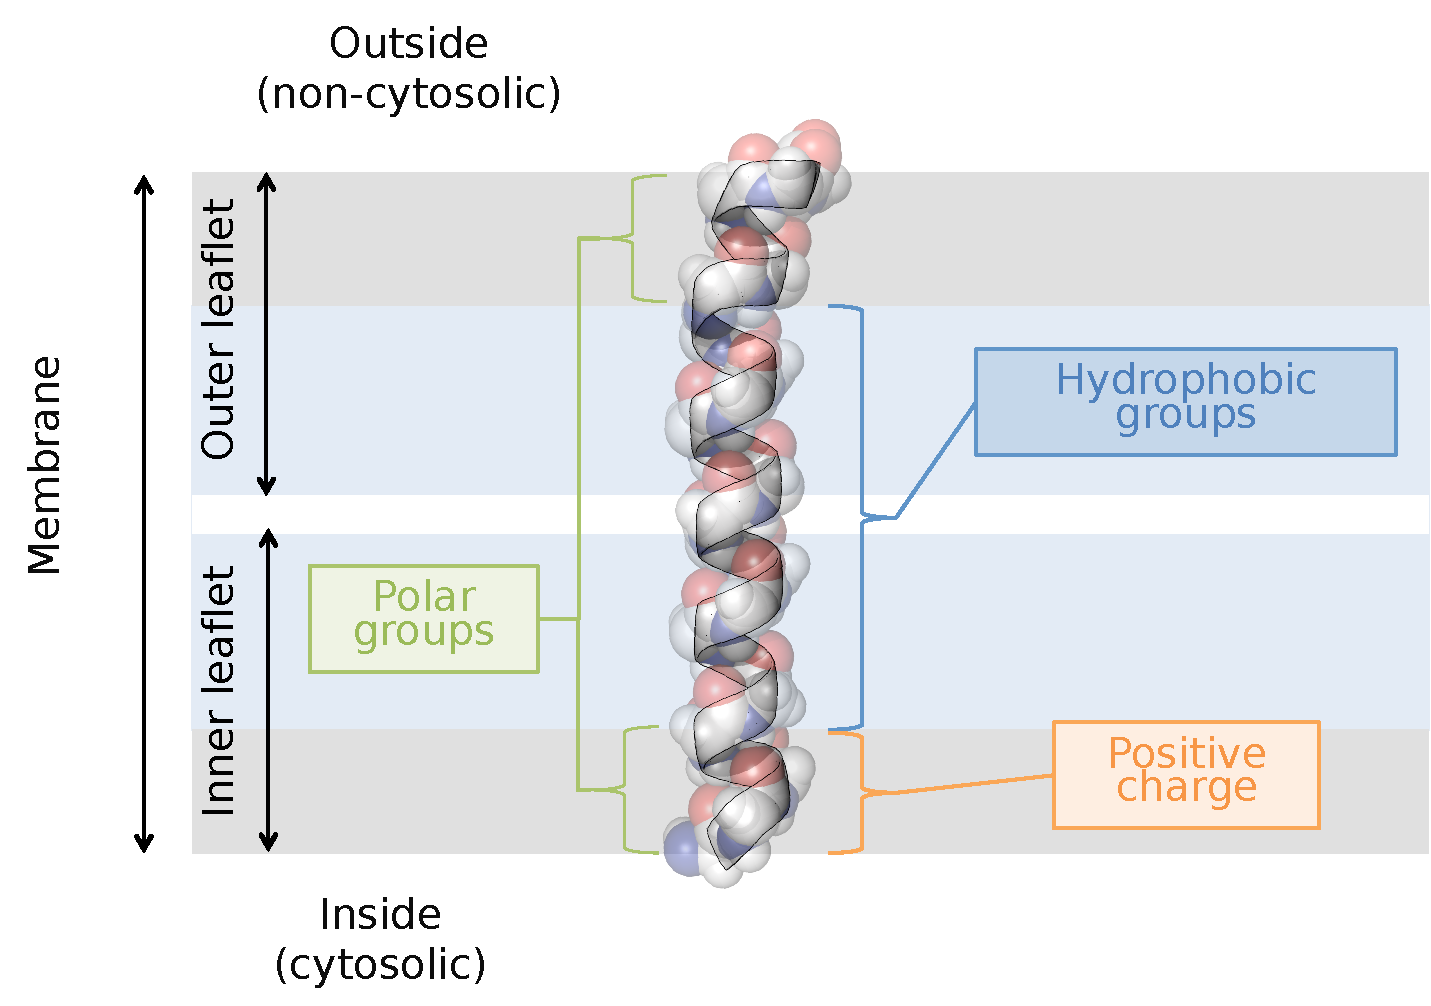
\includegraphics[width=1\textwidth]{Intro/Helix_anatomy}
		\captionof{figure}[A cartoon showing the general components of the membrane and a typical TMH.]{\textbf{A cartoon showing the general components of the membrane and a typical TMH}.
		The example used here for illustrative purposes is the transmembrane region of therein (\gls{pdb} 2LK9)~\cite{Skasko2012}.
		Dark grey areas denote the area of lipid head groups.
		The residues found in these areas are often described as flanking regions and are often in contact with the aqueous interface of the membrane.
		The helix core is mostly composed of hydrophobic residues.
		Although the regions labelled here generally hold true in terms of the statistical distribution of polar, non-polar, and charged groups, it is by no means absolute laws and many proteins break these ``rules''~\cite{Sharpe2010, Baeza-Delgado2013, Pogozheva2013}.}

\label{fig:helixcartoon1}
\end{figure}

% Figure: A cartoon depicting various problematic, yet biologically observed topologies and lengths that the alpha helices can adopt.
From left to right: a typical and traditional \gls{tmh}, an exceptionally long \gls{tmh}, a \gls{tmh} that lies flat in the interface region, a kinked helix that enters and exits the bi-layer on the same leaflet, a \gls{tmh} that is not long enough to span the entire membrane.
These exceptional formations present a challenge for topology predictions of the loop regions.

The language used to describe \gls{tmh}s varies somewhat across the literature, primarily due to a changing understanding of \gls{tmh} general structure and relevance to function over the last 15 years or so.
There is a general composition of a \gls{tmh} despite specific protein and membrane constraints~\cite{Sharpe2010}.

%This paragraph should certainly be changed to the updated one from the manuscript.
A study by Baeza\---Delgado \textit{ et al.} from 2013~\cite{Baeza-Delgado2013} looked at \gls{tmh}s in 170 integral membrane proteins from a manually maintained database of experimentally confirmed \gls{tmp}s; MPTopo~\cite{Jayasinghe2001}.
The group examined the distribution of residues along the \gls{tmh}s.
As expected, half of the natural amino acids are equally distributed along transmembrane (TM) helices whereas aromatic, polar, and charged amino acids along with proline are biasedly near the flanks of the TM helices~\cite{Baeza-Delgado2013}.
It has been noted that transitions between the polar and non-polar groups at the ends of the hydrophobic core occur in a more defined edge on the cytoplasmic side than at the extracytoplasmic face when counting from the middle of the helix outwards~\cite{Baeza-Delgado2013}.
This is probably reflecting the different lipid composition of both leaflets of biological membranes~\cite{Baeza-Delgado2013}.

A previous study by Sharpe \textit{et al.} from 2010 used 1192 human and 1119 yeast predicted \gls{tmh}s that were not structurally validated to further explore the difference in \gls{tmh} and leaflet structure by exploiting the evolutionary conserved sequence differences between the \gls{tmh} in the inner and outer leaflets~\cite{Sharpe2010}.
\gls{tmh}s from vertebrates and invertebrates were found to be reasonably similar compositionally.
The differences in consensus \gls{tmh} structure implies that there are general differences between the membranes of the Golgi and \gls{er}.
The abundance of serines in the region following the lumenal end of Golgi \gls{tms}s probably reflects the fact that this part of many Golgi enzymes forms a flexible linker that tethers the catalytic domain to the membrane~\cite{Sharpe2010}.

\subsubsection{The ``positive\--inside'' rule}

Two publications by von Heijne coined the ``Positive-Inside'' rule demonstrated the practical value of positively charged residue sequence clustering in topology prediction of \gls{tmh}s in bacteria~\cite{VonHeijne1989,Andersson1992}.
It was clearly defined and shown that positively charged residues more commonly were found on the ``inside'' of the cytoplasm rather than the periplasm of \textit{ E.
coli}.
More recently still large-scale sequence analysis of \gls{tmh}s from different organelle membrane surfaces in eukaryotic proteomes, show the clustering of positive charge being cytosolic~\cite{Sharpe2010, Baeza-Delgado2013, Pogozheva2013}.

\subsubsection{The aromatic belt}

Tyrosine and tryptophan residues commonly are found at the interface boundaries of the \gls{tmh} and this feature is called the ``aromatic belt''~\cite{Hessa2005, Granseth2005, Sharpe2010, Baeza-Delgado2013, Nilsson2005a}.
Not all aromatic residues are not found in the aromatic belt; phenylalanine has no particular preference for this region~\cite{Granseth2005, Braun1999}.
However, it still remains unclear if this is to do with anchorage or translocon recognition~\cite{Baeza-Delgado2013}.

A study of conserved tryptophan residues during folding of integrin $\alpha$II$\beta$3 \gls{tm} complex demonstrated the anchoring effects of tryptophan (0.4 kcal/mol contribution to membrane stability) in \gls{tmh}s is greater than the other residues~\cite{Situ2018}. It was suggested that it's wide amphiphilic range (it's stabilising energetic contribution in either hydrophobic or polar sites) complements the heterogeneity and asymmetry of mammalian membrane lipids in particular.

The Tyrosine side chain is a six-membered aromatic ring with an –OH group attached.
Tryptophan has two aromatic rings that are fused into one large hydrophobic ring-structure.
Phenylalanine, although aromatic, is completely hydrophobic, and is found in the transmembrane part rather than the interfacial parts of \gls{tmh}s.
The classical explanation for the preference of Tyrosine and Tryptophan to reside in the interfacial regions is their dipolar character.
The side chain must simply seek compromise.
This can be achieved by burying the aromatic ring close to, or within, the hydrophobic core, while the hydrophilic part can interact with the polar lipid head-groups at the interface.
Other factors such as the aromaticity, size, rigidity and shape of Tryptophan, rather than its dipolar character, has also been suggested as the primary reasons for its interfacial preference.
%Perhaps, as suggested by You \textit{et al.}, it is a balance of all these forces that explains the interfacial preference of Tyrosine and Tryptophan. %This NEEDS referencing!

\subsubsection{Snorkelling}

Broadly speaking, \gls{tmh}s are non-polar.
However, some contain polar and charged residues in the helix itself.
Whilst this might seem thermodynamically unstable at first glance, a molecular dynamic feature called the ``snorkel'' effect explains in part how this is possible~\cite{Chamberlain2004, Strandberg2003}.
Simply put, the snorkelling effect involves the long flexible side chain of leucine reaching the water interface region to interact with the polar head-groups of the bilayer even when the $\alpha$ helix backbone is pulled into the hydrophobic layer~\cite{Krishnakumar2007}.
This has also been suggested to allow helices to adapt to varying thicknesses of the membrane~\cite{Kandasamy2006}.
More recently it was found that although in simulations the energetic cost of arginine at the centre of the \gls{tmh} is large, \textit{in vivo} experimentation with the Sec61 translocon reveals a much smaller penalty~\cite{Ulmschneider2017}.
That same study also found that in \gls{md} simulations, snorkelling, bilayer deformation, and peptide tilting combined to to be sufficient to lower the thermodynamic stability penalty of arginine insertion so that hydrophobic \gls{tmh}s with a central arginine residue will readily insert into the membrane.


\subsection{The hydrophobicity of transmembrane segments}\label{ssection:hydrophobicityscales}

Perhaps the most prevalent and important feature of the transmembrane regions is the membrane spanning region which is composed mostly of non-polar residues.
The importance of hydrophobicity on the effectiveness of membrane anchoring has been known for some time~\cite{Davis1985}.
More recently the hydrophobic group region has been associated with cell localisation and a broad range of biochemical functions~\cite{Junne2010, Sharpe2010, Wong2012}.

Over the last 50 years or so, there have been many attempts to use hydrophobicity scales of residues to predict structural classifications of proteins.
Due to the vast amounts of scales, major efforts have been made to compare them to identify which ones are better for which tasks of identifying structural elements~\cite{Simm2016, Peters2014}.
Simm \textit{ et al.} 2016~\cite{Simm2016} compared 98 scales and found that the accuracy of a scale for secondary structure prediction depends on the spacing of the hydrophobicity values of certain amino acids but generally that the methods behind the scales don't affect the separation capacity between $ \beta $ sheets or $ \alpha $ helices.

Throughout this thesis, several scales are used to evaluate and estimate hydrophobic values of peptide chains.
All the scales aim for quantifying the hydrophobic values of each residue.
There are several key differences in their methodology, assumptions, and aims.
Ultimately, all the scales are attempting to allow estimation of ${\Delta G}_{whf}$; the free energy of a folded helix ($ f $) from the water ($w$) into the membrane core ($h$).
This free energy measurement is regarded as being currently experimentally inaccessible~\cite{Cymer2015}.

Although as a trend most of the scales agree, because of the methodological differences, there are indeed variations of values even after normalisation.
Due to these discrepancies, it is preferable and typical amongst the literature to use several scales to verify the observable trends resulting from interpretation from an individual scale.
Notably, one of the classic scales, Kyte \& Doolittle Hydropathy scale shows a striking similarity to the modern Hessa's ${\Delta G}_{app}^{aa}$ scale, and that generally the ``better'' scales count proline as hydrophilic, and focus on helix recognition rather than amino acid analogues~\cite{Peters2014}.
In $\alpha$ helices from soluble proteins, proline is almost always a helix breaker, and $\alpha$ helix prediction scales don't even attempt to quantify a proline scoring penalty, whereas they are highly tolerated in \gls{tmh}s.
Several of the scales used throughout this thesis are outlined below.

\subsubsection{Kyte \& Doolittle hydropathy scale}

The Kyte \& Dootlittle scale \cite{Kyte1982} is based on the water\---vapour transfer free energy and the interior-exterior distribution of individual amino acids determined previously \cite{Chothia1976}.
The Kyte \& Doolittle gave a composite score to each amino acid based on evidence from previous experiments in the literature, scaling them between -4.5 and +4.5.
These experiments included the molal volumes of model compounds for the side\--chain R groups \cite{Wolfenden1979, Cohn1934, Traube1899}, the water vapour partition coefficients \cite{Hine1975, Wolfenden1979}, and water\--ethanol transfer free energies \cite{Cohn1943, Nozaki1971}.
However alanine, tyrosine, leucine, and proline scores were subjectively modified.
The authors found it difficult to accept that the single methyl group from alanine would have more hydrophobic force than leucine, which contains 4 methyl groups so the score was arbitrarily lowered to half way between the originally determined score, and the score of glycine.
Tyrosine and leucine had their hydropathy values raised to one closer to the water vapour transfer free energy than experimental data suggested.
In the case of proline, no suitable model existed and it tends to become buried, indicating that it is fairly hydrophilic.
However, because it contains three methyl groups, the score considers it more hydrophobic than the experiments suggested.
The authors stated: ``None of these last 3 adjustments, the result of personal bias and heated discussion between the authors, affects the hydropathy profiles in any significant way''\cite{Kyte1982}.
Arginine represents the bottom of the scale, arbitrarily set at -4.5.
An algorithm called SOAP was used to scan a window of $\pm$10 residues either side of each residue (allowing for half windows) across a protein to take the mean average of each position and plot them on a profile.
Sustained areas of high hydrophobicity were indicative of a \gls{tmh}~\cite{Kyte1982}.

\subsubsection{Hessa's biological hydrophobicity scale}
This is arguably the most biologically relevant scale~\cite{Peters2014}, and is often called the ${\Delta G}_{app}^{aa}$ scale.
The scale is based on an experimental method where the free energy exchange during recognition of designed poly-peptide \gls{tmh} by the \gls{er} Sec61 translocon occurred~\cite{Hessa2005}.
These measurements were then used to calculate a “biological hydrophobicity scale.” The original study reported positional variance in some residues and is strictly valid only for residues in the core of the \gls{tmh}.
A more refined study quantified the positional dependencies of each amino acid type~\cite{Hessa2007}.

\subsubsection{White and Wimley octanol \--- interface whole residue scale}
This scale is calculated from two other scales; the octanol scale, and the interface scale~\cite{White1999}.
This scale is fundamentally based on the partitioning of host-guest pentapeptides (acetyl-WL-X-LL-OH) and another set of peptides (AcWLm) between water and octanol, as well as water to \gls{popc}.

\subsubsection{The Eisenberg hydrophobic moment consensus scale}
The Eisenberg scale is a consensus scale based on the earlier scales from Tanford~\cite{Nozaki1971}, Wolfenden~\cite{Rose1993}, Chothia~\cite{Chothia1976}, Janin~\cite{Janin1979},  Wolfenden~\cite{Wolfenden1981}, and the von Heijne scale~\cite{VonHeijne1979}.
The scales are normalised according to serine~\cite{Eisenberg1984}.
The automatic TRANSMEM annotation currently used in UniProt is according to TMHMM~\cite{Krogh2001}, Memsat~\cite{Jones2007}, Phobius~\cite{Kall2004} and the hydrophobic moment plot method of Eisenberg and coworkers~\cite{Eisenberg1984}.

\subsection{Sequence complexity}
Sequence properties that can be analysed by bioinformatics, the sequence complexity and hydrophobicity, of the \gls{tmh} have been used to predict the role of the \gls{tmh} as either functional or structural, and as a discrete cluster from other SCOP annotated helices~\cite{Wong2012}.
Those findings demonstrated that the sequence of the \gls{tmh} holds valuable information regarding biological roles, and forms the basis of our interest in the link between the polarity of a helix and functional activity beyond structural anchorage.

TMSOC's z-score is able to distinguish between functionally active~\gls{tmh}s and those only associated with anchorage~\cite{Wong2011, Wong2012}.
This was determined with annotation of \gls{tmh}s from the UniProt database (303 membrane anchors and 1741 functional TM helices) from UniProt \cite{TheUniProtConsortium2014} and tested with 181132 \gls{tmh} sequences.
Two peaks can be observed when stratifying the hydrophobicity and the sequence complexity of the \gls{tmh}s (Figure \ref{fig:complexity}).
These peaks correspond with the ``simple'' and ``complex'' \gls{tmh} annotation.

\begin{figure}[ht]
\centering
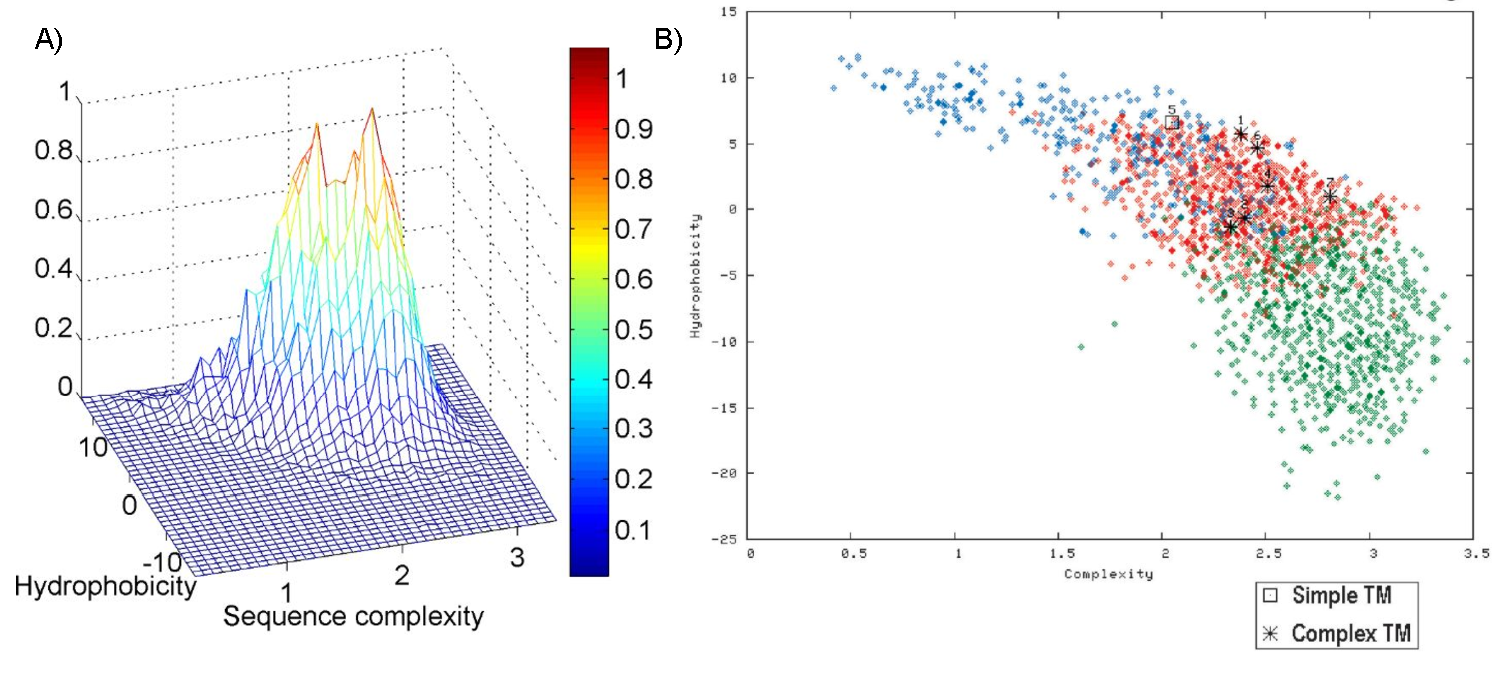
\includegraphics[width=1\textwidth]{Intro/complexity}
		\captionof{figure}[The hydrophobic\--complexity continuum distinguishes between \gls{tmh} anchors, and those with function beyond anchoring.]{\textbf{The hydrophobic\--complexity continuum distinguishes between \gls{tmh} anchors, and those with function beyond anchoring.}
		A) Two distinct points can be observed when plotting sequence complexity on the x axis, frequency on the y axis, and hydrophobiciy on the z axis of \gls{tmh}s from UniProt.
		These peaks were shown to correspond to the membrane anchor and functional \gls{tmh} populations.
		From Wong \textit{et al.,} 2011 \cite{Wong2011}.
		B) The $\protect\alpha$ helix hydrophobicity complexity continuum stratified by hydrophobicity (vertical axis) and complexity (horizontal axis).
		In blue are the membrane anchors, in red are the \gls{tmh} with function, and in green are non\--\gls{tm} $\protect\alpha$ helicess from SCOP \cite{Murzin1995}.
		Clear distinctions can be made between the 3 groups and in fact a composite z-score of the distance of these two factors from the functional \gls{tmh} group allows prediction of which group a \gls{tmh} belongs to \cite{Wong2011, Wong2012}.
		From Wong \textit{et al.,} 2012 \cite{Wong2012}.
		}
\label{fig:complexity}
\end{figure}

The z-score is a product of both hydrophobicity and a Shannon like sequence entropy \cite{Wong2011, Wong2012} of the character string in the~\gls{tmh}. This term is described below in equation~\ref{equation:zscoreterm}.

\begin{equation} \label{equation:zscoreterm}
z({x}_{\Phi},{x}_{c})={(-1)}^{s}\left[\frac{{({x}_{\Phi}-{\mu}_{\Phi})}^{2}}{{\sigma}_{\phi}^{2}}+\frac{{({x}_{c}-{\mu}_{c})}^{2}}{{\sigma}_{c}^{2}}\right]
\end{equation}

Where $x_c$ and $x_\Phi$ are moving window averages of c, the sequence entropy~\cite{Wootton1996}. $\Phi$ is the White and Wimley hydrophobicity~\cite{White1999} for a given segment and $\mu$ and $\sigma$ are the mean and standard deviation of the sequence entropy and hydrophobicity of the functional~\gls{tmh} set, that is those~\gls{tmh}s containing active residues.

Sequence entropy, is essentially an estimate of the linguistic entropy of a string.
In the context of biology can be thought of as an estimation of the non-randomness of a sequence.
Sequence complexity can be used to analyse DNA sequences~\cite{Pinho2013, Oliver1993, Troyanskaya2002}, however here we will focus on the analysis of the complexity of a sequence in protein sequences.

Broadly speaking, the information theory entropy of a linguistic string can be defined as in equation~\ref{simpleentropy}.

\begin{equation} \label{simpleentropy}
	H(S)=-{\sum_{i=1}^n {p_i\log_s(p_i)}}
\end{equation}

Where H is the entropy of a sequence (S), and $p_i$ is the probability of a character $i$ through each position (n) in S. This allows us to quantify the average relative information density held within a string of information~\cite{Shannon1948}.

The compositional complexity is measured over sequence windows. If we have an amino acid composition $\{{{n}_{i}}{\}}_{i}={\min{i}},\ldots,{\max{i}}$ with a window length of $L=\Sigma {n}_i $, the total number of sequences can be calculated by dividing a factorial of the length by the product of the compositions, i.e\  $ N = L!/\Pi{n}_i $ possible sequences.
The SEG algorithm~\cite{WOOTTON1994269, Wootton1996} identifies sub-segments of the raw region which have the lowest probability.
The algorithm searches for and concatenates sub-threshold segments for the Shannon entropy-like term in equation~\ref{shannonentropyliketerm}

\begin{equation} \label{shannonentropyliketerm}
{K}_{2}=-\Sigma\frac{n_i}{L}\log\frac{n_i}{L}
\end{equation}

The lowest probability sub-segment can be defined as $ K_1=\log N/L $.
By altering the window lengths, and the thresholds SEG can be optimised to search for subtle compositional deviations, such as coil-coiled regions.


\section{Biogenesis of transmembrane proteins}
%Depth of secretion pathway (talk about translocons in depth here) & outline post-translational insertion
\subsection{An overview of translocation}
There are, broadly speaking, 3 types of translocation; BiP-mediated eukaryotic post-translational translocation, bacterial post-translational insertion using the Tat system for folded proteins and the Sec system for unfolded proteins, and co-translational insertion in bacteria through the~\gls{htl} protein complex or its individual components.
In this thesis we focus on co\--translation via the Sec pathway, and on post\--translational pathway of \gls{ta} proteins in eukaryotic systems (Figure \ref{fig:post-versus-co-translation}).

\begin{figure}[ht]
\centering
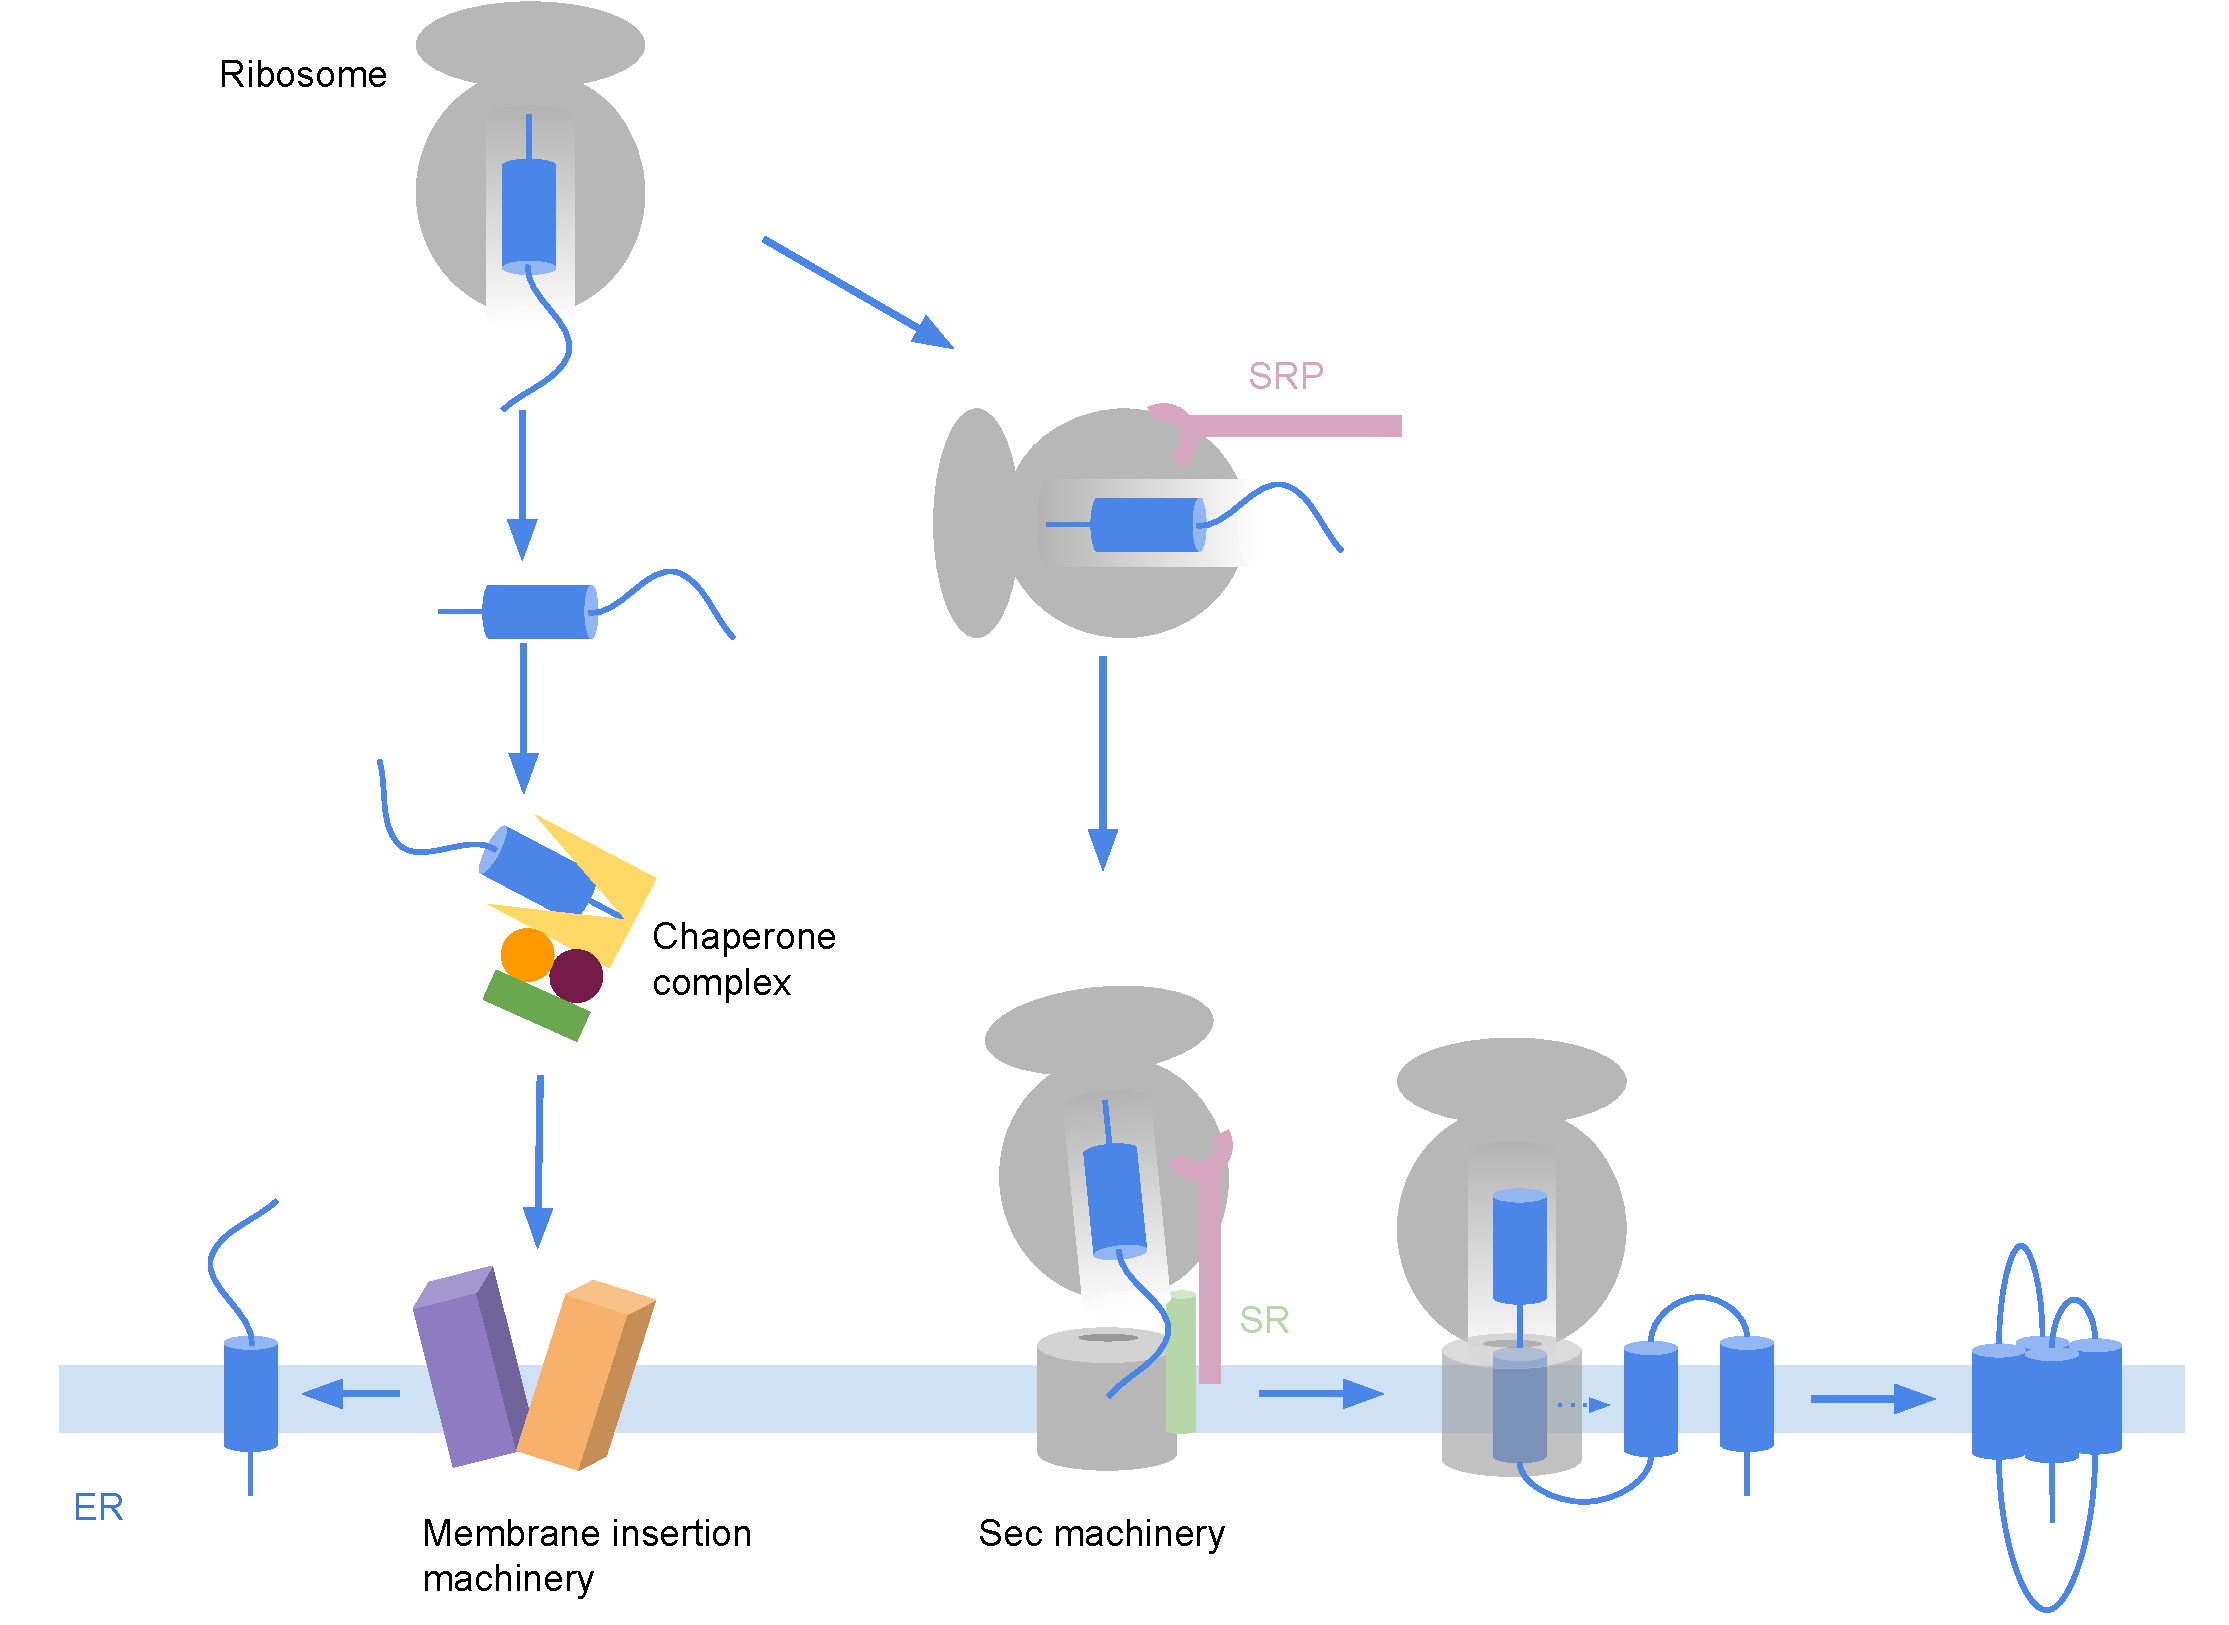
\includegraphics[width=1\textwidth]{Intro/post-versus-co-translation}
		\captionof{figure}[A simplified schematic of the co\--translational Sec pathway and the post\--translational pathway.]{\textbf{A simplified schematic of the co\--translational Sec pathway and the post\--translational pathway.}
		The ribosome translates RNA to a nascent polypeptide chain.
		In the case of post\--translational insertion (the left\--path), the nascent peptide is release, albeit briefly, to the cytosol.
		Chaperones of various types then shield the protein \gls{tmh} and bring it into contact with various \gls{tm} bound translocation machinery.
		In the case of co\--translation (the right\--path), the \gls{srp} binds to the emerging signal sequence of the nascent peptide, which slows protein synthesis of the ribosome.
		\gls{srp} then targets the ribosome protein complex to the \gls{sr}, which then moves into contact with the translocon.
		As the nascent protein is inserted into the translocon, \gls{sr} and \gls{srp} detach from the complex and translocation begins.
		}
\label{fig:post-versus-co-translation}
\end{figure}

The Sec pathway is conserved across all life~\cite{Cao2003} and is facillitated by the SecYEG (prokaryotic) and Sec61 (eukaryotic) translocons.
SecYEG targets proteins to the \gls{pm} (inner membrane) of bacteria.
In bacteria nearly all \gls{tmp}s are inserted by either the Sec pathway via  SecYEG machinery, or by the structurally unrelated the 5\--fold more abundant YidC machinery \cite{Drew2003, Dalby2014}, and proteins can often use either pathway.
Sec61 targets proteins to the \gls{er} of eukaryotic cells.
Broadly speaking, these proteins translocate hydrophilic peptides across a membrane whilst also integrating sufficiently hydrophobic sequences to the membrane~\cite{Junne2010, Rapoport2012, Shao2011, Cymer2015}.
Whilst ultimately the translocon machinery is built of multiple subunits, the \gls{tm} translocating protein itself is a 10 \gls{tmh} protein with an hourglass shaped interior pore~\cite{Berg2004} (SecY in prokaryotes or Sec61$\alpha$ in eukaryotes).
When translocation is not occuring and the protein is idle, the hydrophobic core is constricted~\cite{Junne2010} and a lumenal plug is in place over the pore resulting in a seal across the \gls{tmp} pore~\cite{Tam2005, Junne2006}.
During translocation the plug exits the pore, the constriction ring is opened, and a lateral gate opens between TMH2 and TMH3, and TMH7 and TMH8 to integrate \gls{tmh}s to the membrane~\cite{Berg2004}.
Mutation experiments on these three features (the plug, contriction ring, and lateral gate) destabalised the closed state of the translocon and resulted in a protein localisation phenotype that suppressed inactivating mutations in signal sequences~\cite{Emr1981, Veenendaal2004, Li2007, Junne2007} and even caused transient channel openings in bacteria~\cite{Saparov2007}.
\gls{sp}s in stalled nascent chains crosslinked to the lipid and to the translocon machinery \cite{Martoglio1995}, showing that there may be a holding space which exposes the \gls{tmh} to the membrane  interfacial environment before insertion is complete and this was verified by more recent \gls{em} structural study \cite{Gogala2014, Park2012}.

In bacteria, the SecY protein is partly encircled by SecE which enhances it's stability in the membrane \cite{Kihara1995}
 Sec$\beta$ and Sec$\gamma$

\subsection{Co-translational Translocation}


\subsection{Post-Translational Translocation}
%Remember to point out differences in pro and eukaryotes.

\subsection{Signal peptides}
\gls{sp}s are short peptide sequences present at the N-terminus of most secretory pathway destined proteins in both prokaryotes and eukaryotes.
Mutations to the length and compostion of the \gls{sp} revealed their composition is essential for effective localised transport, however they have high compositional variability \cite{VonHeijne1985}.
Like \gls{tmh}s they translocate into the membrane due to their hydrophobic $\alpha$ helix (albeit typically shorter than a \gls{tmh}) and follow the positive\--inside rule.

\begin{figure}[ht]
\centering
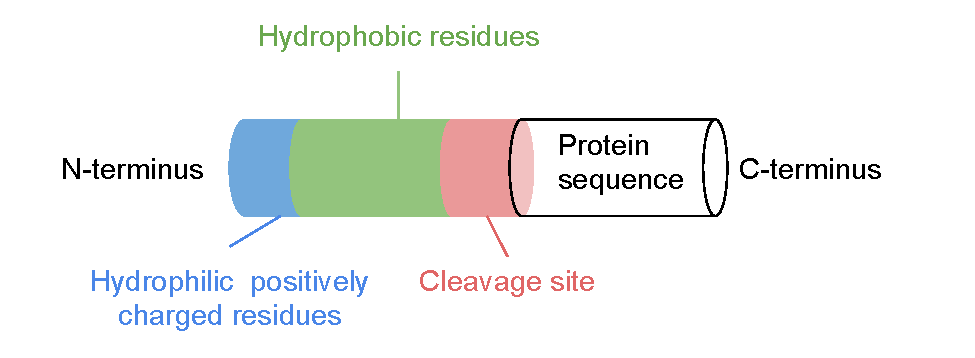
\includegraphics[width=1\textwidth]{Intro/sp}
		\captionof{figure}[They key components of a signal peptide.]{\textbf{They key components of a signal peptide.}
		Signal peptides consist of between 1\--5 hydrophilic charged residues (in blue) at the N terminal, a 7-15 reisude hydrophobic region (in green), and a c-region of 3-7 residues that invites cleavage by specific signal peptidase (in red).
	Adapted from von Heijne, 1990 \cite{VonHeijne1990}.
		}
\label{fig:sp}
\end{figure}


Once the protein is fully translocated and at the correct location within the cell, a three domain signal peptidase cleaves the \gls{sp} from the rest of the protein.
\gls{sp}s can also be experimentally interchanged to proteins from different organisms to target them to cellular locations \cite{Izard1994, Gierasch1989}.

\gls{sp}s are rarely used by \gls{tmp}s with the exception of most type I \gls{tmp}s, which are defined by the presence of an \gls{sp}.
Instead, \gls{tmp}s use their first \gls{tmh} and flanking region as a targetting signal.
Many bioinformatic methods over the last twenty years have aimed to predict \gls{sp}s and sort them from \gls{tmh}s \cite{Choo2009}, however these methods all struggle to distinguish \gls{sp}s from N-terminal \gls{tmh}s \cite{Petersen2011}.
This is due to the similarities \gls{sp}s have with gls{tmh}s, and that although \gls{tmh}s are not cleaved, the cleavage site pattern alone cannot effectively separate \gls{sp}s from \gls{tmh}s.
This results in many false positives for \gls{sp} presence in genome wide studies \cite{Petersen2011}.
SignalP 4, a neural network based approach, is less effective at predicting cleavage sites or \gls{sp} prediction in the absence of \gls{tmp}s from the dataset, however currently is the most accurate method to distinguish the currently vague differences between \gls{tmh}s and \gls{sp}s \cite{Petersen2011}.

\subsection{$\protect\beta$ sheets in the membrane}

The membrane is critical in maintaining the separation of biochemically distinct compartments.
However, there needs to be flux of not only molecules, but information signals across these membranes in order to facillitate cellular life.
Whilst the focus of this thesis is primarily on \gls{tmh}s it is important to acknowledge that $\beta$ sheets are another secondary structural element capable of spanning the membrane.

\begin{figure}[ht]
\centering
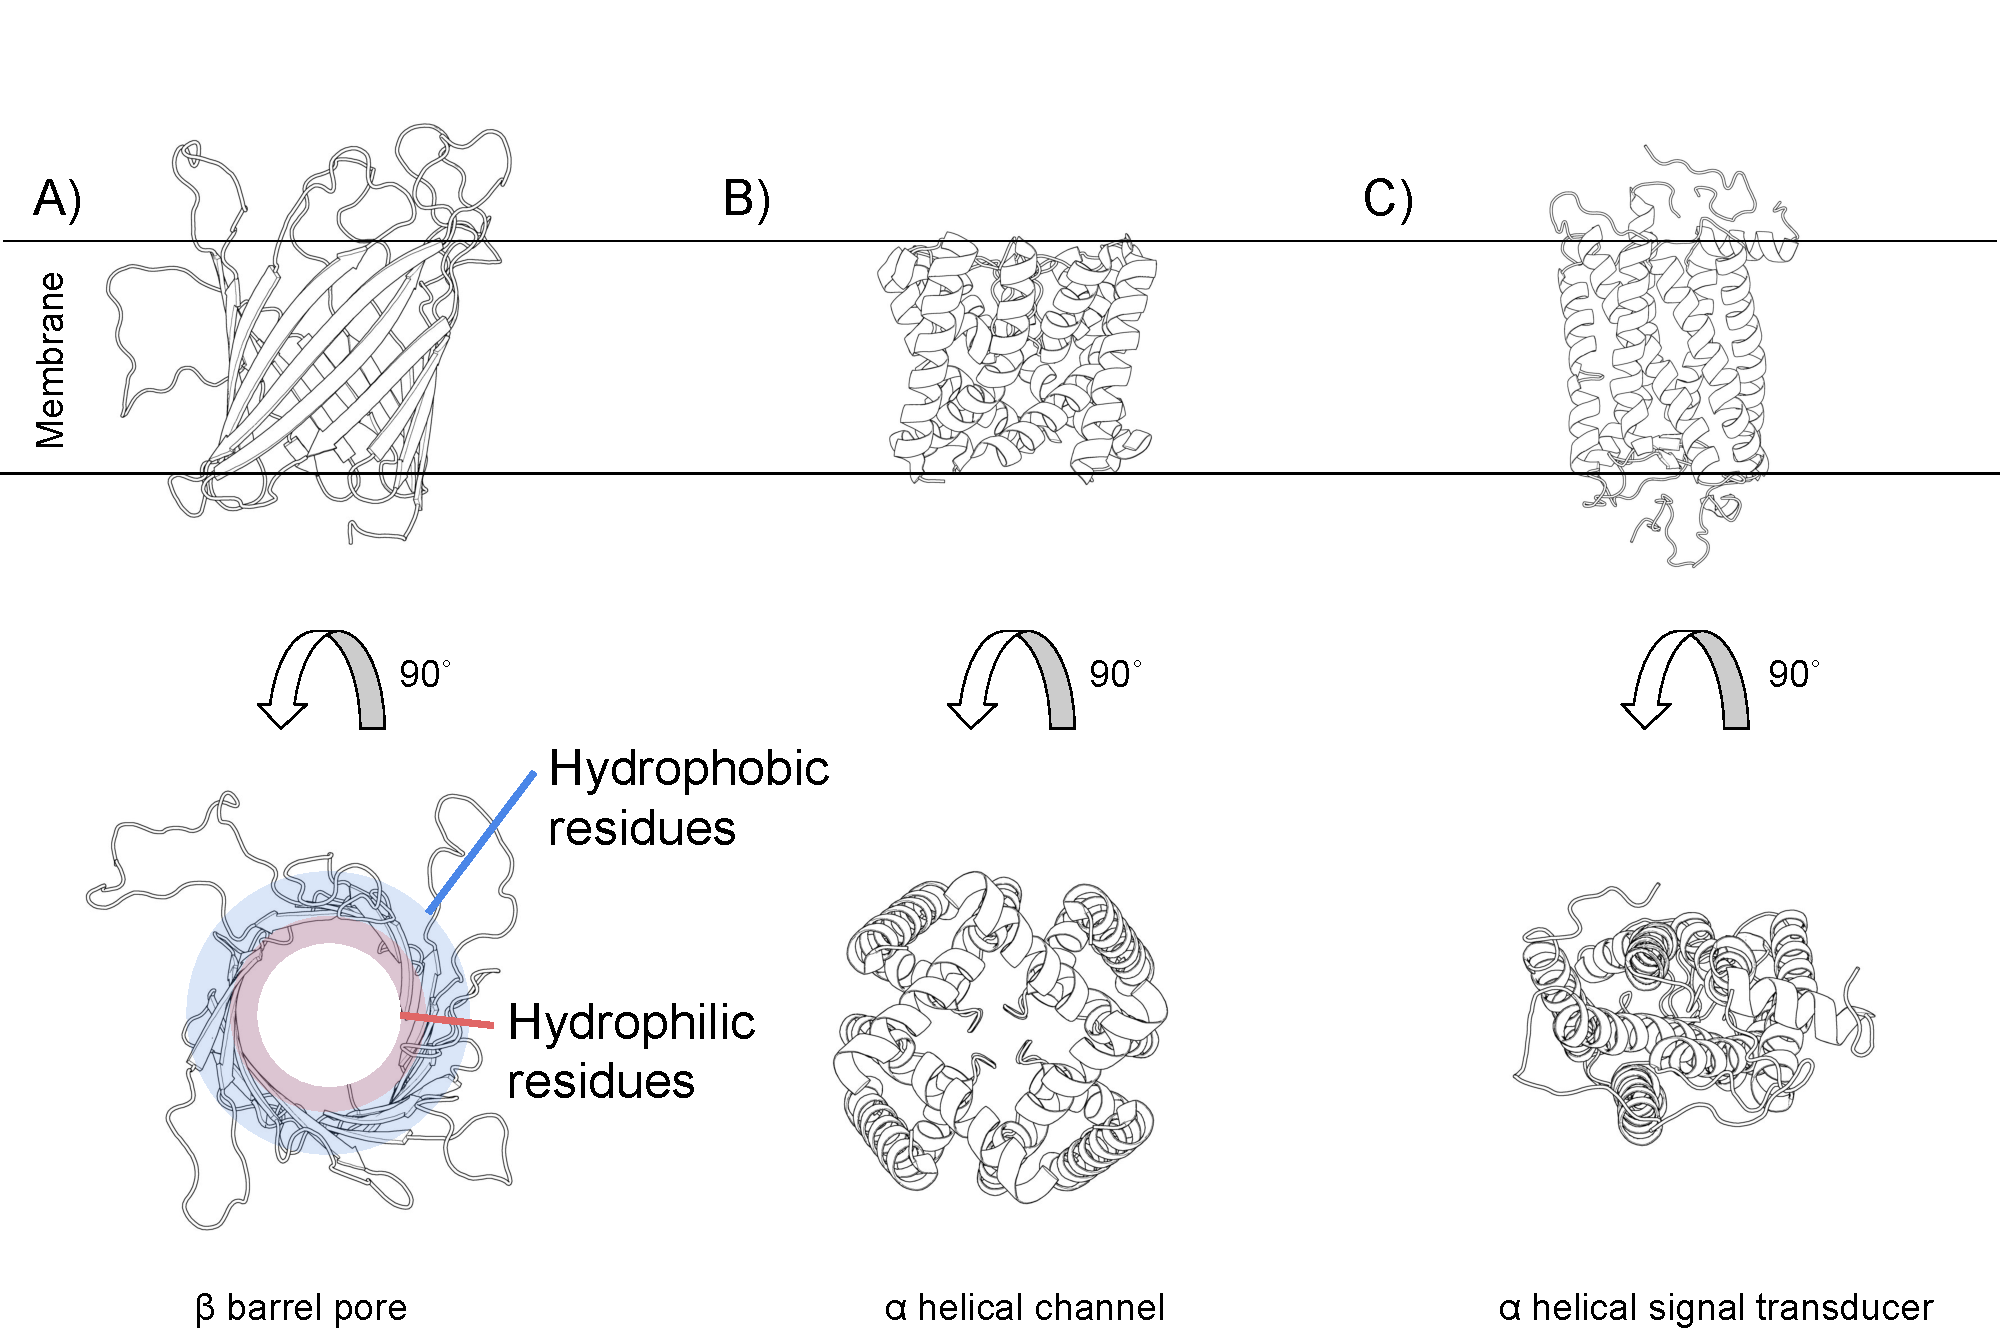
\includegraphics[width=1\textwidth]{Intro/barrel-versus-helix}
		\captionof{figure}[Cartoons showing the structural differences of the outer membrane $\protect\beta$\--barrel proteins, transmembrane $\protect\alpha$\--helix channels, and transmembrane $\protect\alpha$\--helix signal transducers in the membrane.]{\textbf{Cartoons showing the structural differences of the outer membrane proteins, transmembrane helix channels, and transmembrane helix signal transducers in the membrane.}
		The top row shows the proteins traversing the membrane with the interfacial regions denoted by the black lines.
		A) A porous outer membrane protein using $\protect\beta$\--sheets to form a pore\--forming protein structure.
		PDB code 2JQY.
		B) A highly selective ion channel made up of membrane spanning \gls{tmh}s.
		PDB code 4HYO.
		C) A 7\--\gls{tmh} \gls{gpcr} that recieves a signal on one side of the membrane which causes a conformational change influencing the structural arrangement of the tertiary structure on the opposing side of the membrane.
		PDB code 1F88.
		Note the pore in the $\protect\beta$ barrel protein not present in either the \gls{tmh} channel or the \gls{tmh} transducer.
		}
\label{fig:barrel-versus-helix}
\end{figure}

$\beta$ barrel proteins are present only in a few membrane types; the outer membrane of Gram negative bacteria for which they constitute between 2-3\% of the genome \cite{Wimley2003}, and in the outer membranes of eukaryotic chloroplasts and mitochondrial membranes.
Their restriction to these membrane types is the result of ancestral symbiogenesis \cite{McFadden2001, Gray1999, Fischer1994, Zeth2010, Fairman2011, Ulrich2015}.

These outer membrane proteins cause the membranes to be permeable, diminishing membrane potential between the outer and the inner membrane.
Unlike the \gls{tmh}s, $\beta$ barrel proteins are permeable to water and many other small molecules often unspecifically due to their large pore (Figure \ref{fig:barrel-versus-helix}).
Integral $\beta$ barrel proteins consist of between 8 and 26 apmphipathic antiparallel $\beta$ strands forming a cylindrical pore.
They are capable of active and passive transport, molecule receptors, enzymatic catalysis, structural formation, and translocon machinery \cite{Wimley2003}.

The biogenesis of $\beta$ barrel membrane proteins also differs from that of \gls{tmh}s, and there are differences between prokaryotic and eukaryotic cells.

In Gram negative bacteria, the $\beta$ barrel proteins are translated on cytoplasmic ribosomes (Figure \ref{fig:beta-mito-versus-bacteria}).
An N-terminal \gls{sp} sequence allows the protein to pass through the inner membrane to the outer membrane \cite{Driessen2008, Papanikou2007}.
Instead of cotranslational insertion, SecB transports the nascent polypeptide chain to the Sec translocon on the inner membrane \cite{Bechtluft2010}.
$\beta$\--sheets do not trigger the opening of the lateral gate \cite{Ulrich2015}.
Once in the periplasm the \gls{sp} is cleaved \cite{Paetzel2014} and chaperones, such as the redundant SurA \cite{Lazar1996, Volokhina2011}, DegQ, and Skp \cite{Volokhina2011}, bind to the protein to prevent premature folding.
Once at the inner-surface, the BAM complex assembles and integrates the $\beta$ barrel protein into the membrane \cite{Wu2005, Hagan2011} via a lateral opening of one of the BAM subunits, BamA \cite{Noinaj2014}.

\begin{figure}[ht]
\centering
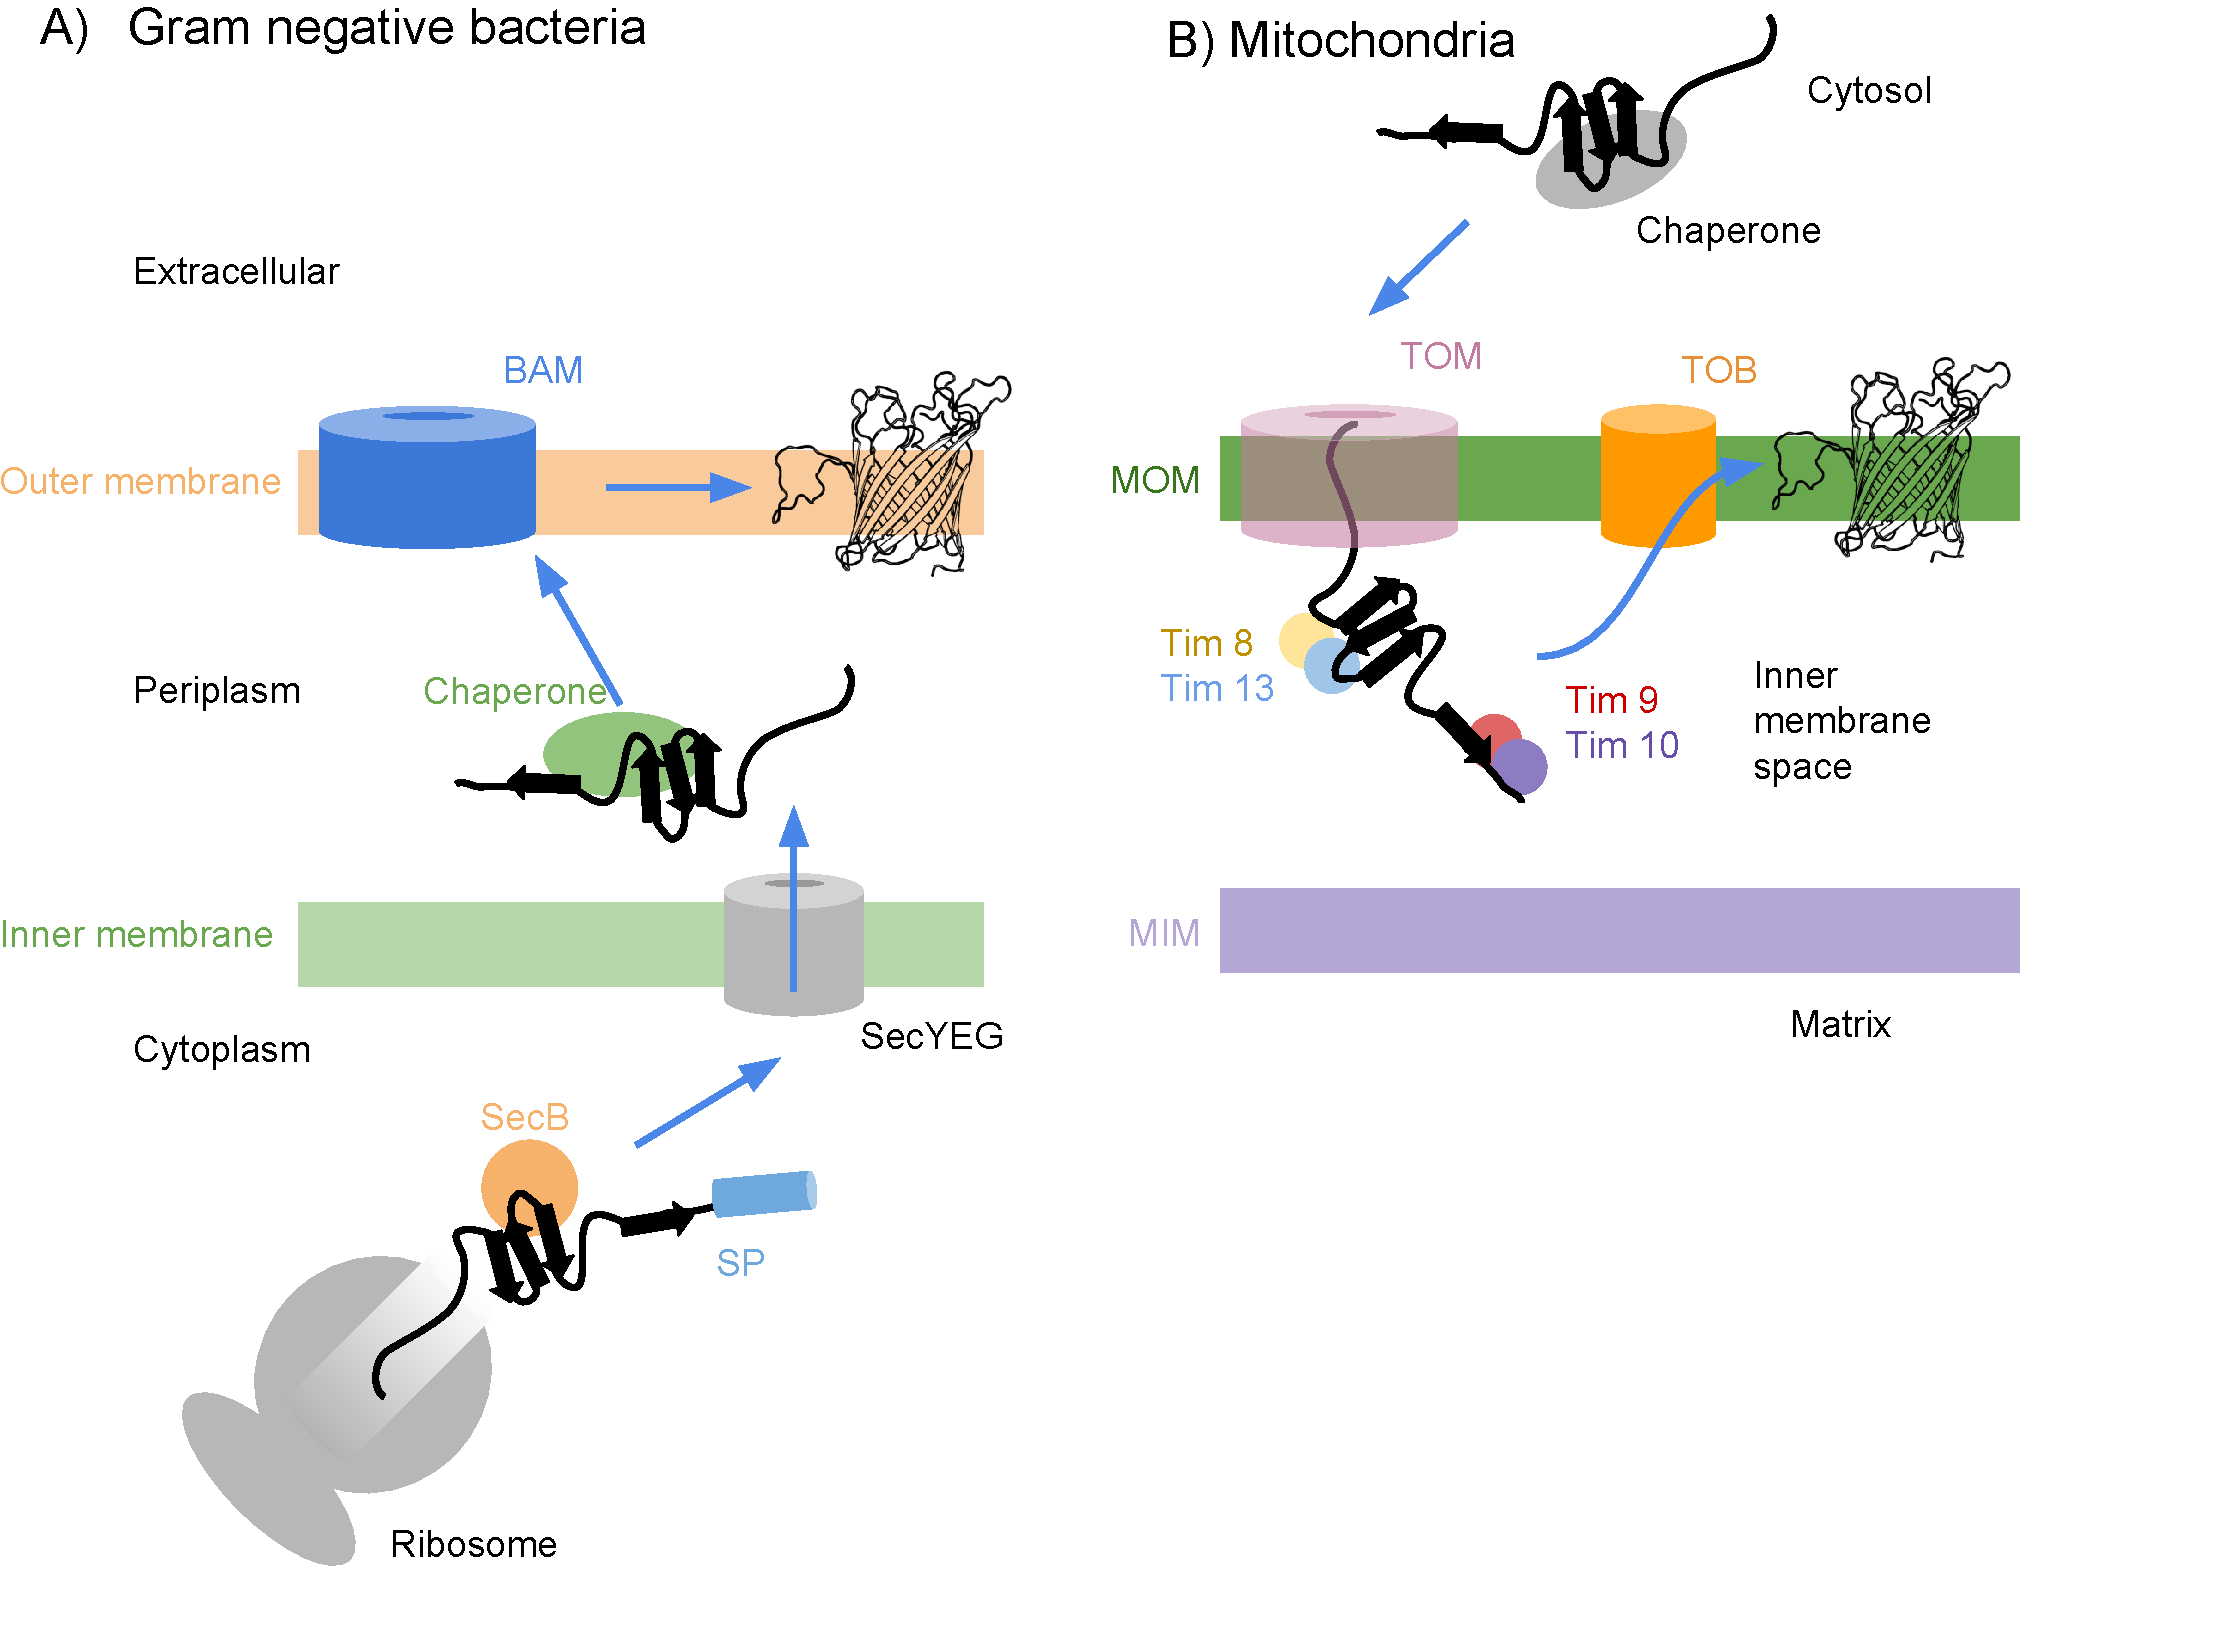
\includegraphics[width=1\textwidth]{Intro/beta-mito-versus-bacteria}
		\captionof{figure}[A cartoon of the biogenesis of $\protect\beta$ barrel membrane proteins in mitochondria and Gram\--negative bacteria.]{\textbf{A cartoon of the biogenesis of $\protect\beta$ barrel membrane proteins in mitochondria and Gram\--negative bacteria.}
		This is an overview of the current model of $beta$ barrel protein membrane integration.
		A)In bacteria, SecB chaperones the nascent peptide to SecYEG where it is transported across the inner membrane.
		Once the \gls{sp} is cleaved, the protein is chaperoned to the BAM machinery by SurA, DegQ, or Skp.
		The BAM machinery integrates the protein into the membrane.
		B)After ribosomal translation the nascent peptide is transported across the mitochondrial outer membrane by the \gls{tom} machinery.
		Several Tim recognition molecules then attach to the protein and present it to the TOB insertion machinery, which integrates the protein into the membrane.
		Adapted from Ulrich \& Rapoport, 2015 \cite{Ulrich2015}.

		}
\label{fig:beta-mito-versus-bacteria}
\end{figure}

Unlike in the bacterial outer membrane, $\beta$-barrel proteins are rare in the mitochondria \cite{Ulrich2015}.
There is Tom40, Tob55, two isoforms of a porin, and Mdm10 \cite{Ulrich2015}.
And yet, indeed it was shown that a $\beta$ barrel protein fragments not found in the eukaryotic proteome called trimeric autotransporter can be recognised and assembled byt the mitochondria \cite{Muller2011}.
Since there is no need to cross the inner membrane, mitochondrial proteins do not have the cleavable \gls{sp}, or any other known targetting signal \cite{Ulrich2015}.
After cytosolic ribosomes complete the translation, the $\beta$ barrel proteins are recognised on the mitochondrial surface by the \gls{tom} complex import receptors, handed to the $\beta$ barrel protein Tom40 which is the central machinery for mitochondrial protein import \cite{Chachinska2009}.
After being processed through the \gls{tom} machinery, hexameric chaperone complexes of Tim8 in complex with Tim13, and Tim9 in complex with 10 to the TOB complex (also known as the SAM complex) also on the outer membrane which integrates the $\beta$ barrel protein into the membrane \cite{Wiedermann2003, Paschen2003, Gentle2004}.

Whereas mitochondria originated from the ancestral incorporation of $\alpha$\--proteobacteria \cite{Gray1999}, chloroplasts were thought to originate from the incorporation of cyanobacterium \cite{McFadden2001}.
Similarly to mitochondrial $\beta$ barrel proteins, there is no cleavable targetting \gls{sp} targetting for the chloroplast since they integrate on the internal side of the membrane, however much less is known about the precise insertion machinery of $\beta$ barrel proteins at a molecular level in chloroplasts \cite{Ulrich2015}.

Besides the differences in biogenesis between $\beta$ barrel \gls{tmp}s and \gls{tmp}s with \gls{tmh}s as the membrane spanninging units, there are also biophysical differences.
Membrane spanning $\beta$ sheets exhibit a ``positive\--outside'' distribution of positively charged residues \cite{Pogozheva2013}, opposed to the much more typical positive\--inside distribution \cite{VonHeijne1989, Andersson1992, Pogozheva2013, Sharpe2010, Baeza-Delgado2013}.
Typically, $\beta$ sheets are less hydrophobic than \gls{tmh}s \cite{Tamm2004} as a result of their amphiphilic nature.

\section{The aims of this thesis.}

In this thesis we explore three ideas surrouding the role of \gls{tmh}s in the membrane.

In chapter 2 we explore the sequence composition of large datasets of \gls{tmh}s straifying them by species, organelle, single\--pass and multi\--pass.
After considering the rarity of certain amino acid types, we ellucidate a ``negative\--outside'' tendency in concert with the positive\--inside rule.
We go on to further divide the single\--pass group into complex and simple \gls{tmh}s according to TMSOC.
This reveals that simple \gls{tmh}s have amino acid distribution features along the helix that would optimise for anchoring, however complex \gls{tmh}s are more akin to \gls{tmh}s from multi\--pass \gls{tmp}s.

In chapter 3 we generate an up to date dataset of post\--translationally inserted \gls{ta} proteins based on previous methods and compare the \gls{tmh}s within to a manually curated \gls{ta} protein dataset from UniProt.
This cross examination revealed \gls{tmh} adaptaions to mitochondrial membranes such as a reversal of the ``positive\--inside'' rule and a reduction in hydrophobicity caused by an abundance of alanine residues in lieu of leucine rather than an increase of polar residues.
We also generate homology models of two spontanously inserting \gls{tmh}s from \gls{ta} proteins and show that they have an amphiphatic surface which may be key to their insertion.

In chapter 4 we look at families of \gls{tmp}s that exhibit high hydrophobic discrepency between sequentially adjacent \gls{tmh}s.
The conservation of these pairs across the families corroborates evidence of cooperative \gls{tmh} insertion, showing that marginally hydrophobic \gls{tmh}s could use typical \gls{tmh}s as part of their biogenesis on a larger scale than previously thought.

\chapter{The ``Negative-Outside'' rule.}
\sloppy
The description of a~\gls{tmh} remains incomplete.
The understanding of~\gls{tmp} topology is erroneous, and despite a wealth of structures, the general model of helix-helix and helix-lipid interactions remains speculative and requires a great deal of intensive analysis to generate a working model of a particular~\gls{tmp}.

The work presented in this chapter is an expanded version of published work~\cite{Baker2017}.
We use advanced statistical analysis to analyse large sequence datasets that have rich topological annotation.
By analysing these sequences in the context of anchorage, we find that some~\gls{tmh}s are confined to biological constraints of the membrane, whereas others that likely contain function beyond anchorage, are less conforming to the membrane.
Specifically, there is further elaboration of statistical definitions in the methods than in the published paper.

\section{Abstract}

\section{Summary}
As the idea of positive residues inside the cytoplasm emerged during the late 1980s, so did the idea of negative residues working in concert with~\gls{tmh} orientation.
It was shown that removing a single lysine residue reversed the topology of a model \textit{erichia coli} protein, whereas much higher numbers of negatively charged residues are needed to reverse topology~\cite{Nilsson1990}.
One would also expect to see a skew in negatively charged distribution if a cooperation between oppositely charged residues orientated a~\gls{tmh}, however there is no conclusive evidence in the literature for an opposing negatively charged skew~\cite{Granseth2005, Nilsson2005a, Sharpe2010, Baeza-Delgado2013, Pogozheva2013}.
However, in \textit{E.
coli} negative residues do experience electrical pulling forces when travelling through the SecYEG translocon indicating that negative charges are biologically relevant~\cite{Ismail2015}.
In this chapter, we explore the literature surrounding charged residue distribution in the~\gls{tmh}, and demonstrate that the ``negative-outside'' skew exists in anchoring~\gls{tmh}s

\section{Introduction}

Two decades ago, the classic concept of a~\gls{tmh} was a rather simple story: Typical~\gls{tmp}s were thought to be anchored in the membrane by membrane-spanning bundles of non-polar \(\alpha\)--helices of roughly 20 residues length, with a consistent orientation of being perpendicular to the membrane surface.
Although this is broadly true, hundreds of high quality membrane structures have elucidated that membrane-embedded helices can adopt a plethora of lengths and orientations within the membrane.
They are capable of just partial spanning of the membrane, spanning using oblique angles, and even lying flat on the membrane surface~\cite{Elofsson2007, VonHeijne2006}.
The insertion and formation of the~\gls{tmh}s follow a complex thermodynamic equilibrium~\cite{Moon2013, MacCallum2011, Cymer2015}.
From the biological function point of view, many~\gls{tmh}s have multiple roles besides being just hydrophobic anchors; for example, certain~\gls{tmh}s have been identified as regulators of protein quality control and trafficking mechanisms~\cite{Hessa2011}.
As these additional biological functions are mirrored in the~\gls{tmh}s’ sequence patterns,~\gls{tmh}s can be classified as simple (just hydrophobic anchors) and complex sequence segments~\cite{Wong2010, Wong2011, Wong2012}.

The relationship between sequence patterns in and in the vicinity of~\gls{tmh}s and their structural and functional properties, as well as their interaction with the lipid bilayer membrane, has been a field of intensive research in the last three decades~\cite{Ladokhin2015}.
Besides the span of generally hydrophobic residues in the~\gls{tmh}, there are other trends in the sequence such as with a saddle-like distribution of polar residues (depressed incidence of charged residues in the~\gls{tmh}  itself), an enriched occurrence of positively charged residues in the cytosolic flanking regions as well as an increased likelihood of tryptophan and Tyrosine at either flank edge~\cite{Sharpe2010, VonHeijne1986,VonHeijne1988,VonHeijne1989, Baeza-Delgado2013, Granseth2005}.
Such properties vary somewhat in length and intensity between various biological organelle membranes, between prokaryotes and eukaryotes~\cite{Ojemalm2013} and even among eukaryotic species studied due to slightly different membrane constraints~\cite{Sharpe2010, Pogozheva2013}.
These biological dispositions are exploitable in terms of~\gls{tm} region prediction in query protein sequences~\cite{Beuming2004, Zhao2006} and tools such as the quite reliable TMHMM~\cite{Krogh2001,Sonnhammer1998}, Phobius~\cite{Kall2004, Kall2007} or DAS-TMfilter represent today’s prediction limit of~\gls{tmh}s’ hydrophobic cores within the protein sequence~\cite{Cserzo2002, Cserzo2004, Kall2002}.
The prediction accuracy for true positives and negatives is reported to be close to 100\% and the remaining main cause of false positive prediction are hydrophobic \(\alpha\)--helices completely buried in the hydrophobic core of proteins.
 To note, reliable prediction of~\gls{tmh}s and protein topology is a strong restriction for protein function of even otherwise non\-characterised proteins~\cite{Eisenhaber2016, Eisenhaber2012, Sherman2015} and thus, very valuable information.

The ``positive\-inside rule'' reported by von Heijne~\cite{VonHeijne2006,VonHeijne1989} postulates the preferential occurrence of positively charged residues (lysine and arginine) at the cytoplasmic edge of~\gls{tmh}s.
The practical value of positively charged residue sequence clustering in topology prediction of~\gls{tmh} was first shown for the plasmalemma in bacteria~\cite{VonHeijne1989, Sipos1993}.
As a trend, the ``positive-inside rule'' has since been confirmed with statistical observations for most membrane proteins and biological membrane types~\cite{Baeza-Delgado2013, Gavel1991, Nilsson2005a, Wallin1998}.
However, more recent evidence suggests that, in thylakoid membranes, the ``positive-inside rule'' is less applicable due to the co-occurrence of aspartic acid and glutamic acid residues together with positively charged residues~\cite{Pogozheva2013}.

The positive-inside rule also received support from protein engineering experiments that revealed conclusive evidence for positive charges as a topological determinant~\cite{VonHeijne1989, Beltzer1991, Kida2006, Nilsson1990}.
Mutational experiments demonstrated that charged residues, when inserted into the centre of the helix, had a large effect on insertion capabilities of the~\gls{tmh} via the translocon.
Insertion becomes more unfavourable when the charge was placed closer to the~\gls{tmh} core~\cite{Hessa2005}.

It remains unclear exactly why and how exactly the positive charge determines topology from a biophysical perspective.
Positively charged residues are suggested to be stronger determinants of topology than negatively charged residues due to a dampening of the translocation potential of negatively charged residues.
This dampening factor is the result of protein-lipid interactions with net zero charged phospholipid, phosphatidylethanolamine and other neutral lipids.
This effect favours cytoplasmic retention of positively charged residues~\cite{Bogdanov2014}.

The recent accumulation of~\gls{tmp} sequences and structures allowed revisiting the problem of charged residue distribution in~\gls{tmh}s (see also \url{http://blanco.biomol.uci.edu/mpstruc/}).
For example, whilst \(\beta\)--sheets contain charged residues in the~\gls{tm} region, α-helices generally do not (38).
Large-scale sequence analysis of~\gls{tmh} from various organelle membrane surfaces in eukaryotic proteomes confirm the clustering of positive charge having a statistical bias for the cytosolic side of the membrane.
At the same time, there are many~\gls{tmh} exception examples to the positive-inside rule; however as a trend, topology can be determined by simply looking for the most positive loop region between helices~\cite{Sharpe2010, Baeza-Delgado2013}.

When the observation of positively charged residues preferentially localised at the cytoplasmic edge of~\gls{tmh}s emerged, it was also asked whether negatively charged residues work in concert with~\gls{tmh} orientation.
It was shown that a single additional lysine residue can reverse the topology of a model \textit{Escherichia coli} protein, whereas a much higher number of negatively charged residues is needed to achieve the same~\cite{Nilsson1990}; nevertheless, a sufficiently large negative charge can overturn the positive-inside rule~\cite{Andersson1993, Kim1994} and, thus indeed, negative residues are topologically active to a point.
Negatively charged residues were observed in the flanks of~\gls{tmh}s~\cite{Baeza-Delgado2013}, especially of marginally hydrophobic~\gls{tm} regions~\cite{Delgado-Partin1998}.
It is known that the negatively charged acidic residues in~\gls{tm} regions have a non-trivial role in the biological context.
In \textit{E.
coli}, negative residues experience electrical pulling forces when travelling through the SecYEG translocon indicating that negative charges are biologically relevant during the electrostatic interactions of insertion~\cite{Ismail2012, Ismail2015}.

Unfortunately, there is a problem with statistical evidence for preferential negative charge occurrence next to~\gls{tmh} regions.
Early investigations indicated overall both positive and negative charge were influential topology factors, dubbed the charge balance rule.
If true, one would also expect to see a skew in the negative charge distribution if a cooperation between oppositely charged residues orientated a~\gls{tmh}~\cite{Sipos1993, Hartmann1989}.
It might be expected that, if positive residues force the loop or tail to stay inside, negative residues would be drawn outside and topology would be determined not unlike electrophoresis.
Yet, there is plenty of individual protein examples but no conclusive statistical evidence in the current literature for a negatively charged skew~\cite{Sharpe2010, Baeza-Delgado2013, Granseth2005, Pogozheva2013, Nilsson2005a, Andersson1992}.

There are many observations described in the literature that charged residues determine topology more predictably in single-pass proteins than in multi-pass~\gls{tmh}~\cite{Kim1994, Harley1998}.
It is thought that the charges only determine the initial orientation of the~\gls{tmh} in the biological membrane; yet, the ultimate orientation must be determined together with the totality of subsequent downstream regions~\cite{Sato1998}.

With sequence-based hydrophobicity and volume analysis and consensus sequence studies, Sharpe \textit{et al.}~\cite{Sharpe2010} demonstrated that there is asymmetry in the intramembranous space of some membranes.
Crucially, this asymmetry differs among the membrane of various organelles.
They conclude that there are general differences between the lipid composition and organisation in membranes of the Golgi and~\gls{er}.
Functional aspects are also important.
For example, the abundance of serines in the region following the lumenal end of Golgi~\gls{tmh}s appears to reflect the fact that this part of many Golgi enzymes forms a flexible linker that tethers the catalytic domain to the membrane~\cite{Sharpe2010}.

A study by Baeza-Delgado \textit{et al.}~\cite{Baeza-Delgado2013} analysed the distribution of amino acid residue types in~\gls{tmh}s in 170 integral membrane proteins from a manually maintained database of experimentally confirmed~\gls{tmp}s (MPTopo~\cite{Jayasinghe2001}) as well as in 930 structures from the~\gls{pdb}.
As expected, half of the natural amino acids are equally distributed along~\gls{tmh} whereas aromatic, polar and charged amino acids along with proline are biased near the flanks of the TM helices.
Unsurprisingly, leucine and other non-polar residues are far more abundant than the charged residues in the~\gls{tm} region~\cite{Sharpe2010}.

In this work, we revisit the issue of statistical evidence for the preferential distribution of negatively charged (and a few other) residues within and nearby~\gls{tmh}s.
We rely on the improved availability of comprehensive and large sequence and structure datasets for~\gls{tm} proteins.
We also show that several methodical aspects have hindered previous studies~\cite{Sharpe2010, Baeza-Delgado2013, Pogozheva2013} to see the consistent non-trivial skew for negatively charged residues disfavouring the cytosolic interfacial region and/or preferring the outside flank.
First, we show that acidic residues are especially rare within and in the close sequence environment of~\gls{tmh}s, even when compared to positively charged lysine and arginine.
Second, therefore, the manner of normalisation is critical: Taken together with the difficulty to properly align~\gls{tmh}s relative to their boundaries, column-wise frequency calculations relative to all amino acid types as in previous studies will blur possible preferential localisations of negative charges in the sequence.
However, the outcome changes when we ask where a negative charge occurs in the sequence relative to the total amount of negative charges in the respective sequence region.
Thus, by accounting for the rarity of acidic residues with sensitive normalisation, the ``non-negative inside rule/negative-outside rule'' is clearly supported by the statistical data.
We find that minor changes in the flank definitions such as taking the~\gls{tmh} boundaries from the database or by generating flanks by centrally aligning~\gls{tmh}s and applying some standardised~\gls{tmh} length does not have a noticeable influence on the charge bias detected.

Third, there are significant differences in the distribution of amino acid residues between single-pass and multi-pass~\gls{tm} regions in both the intra-membrane helix and the flanking regions with further variations introduced by taxa and by the organelles along the secretory pathway.
Importantly, we find that it is critical to weigh down the effect of~\gls{tmh}s in multi-pass~\gls{tmp}s with no or super-short flanks to observe statistical significance for the charge bias.
To say it bluntly, if there are no flanks of sufficient length, there is also no negative charge bias to be observed.

The charge bias effect is even clearer when a classification of~\gls{tmh}s into so-called simple (which, as a trend, are mostly single-pass and mere anchors) and so-called complex (which typically have functions beyond anchorage) is considered~\cite{Wong2010, Wong2011, Wong2012}.
We also observe parallel skews with regard to leucine, tyrosine, tryptophan and cysteine distributions.
With these large-scale datasets and a sensitive normalisation approach, new sequence features are revealed that provide spatial insight into~\gls{tmh} membrane anchoring, recognition, helix-lipid, and helix-helix interactions.

\section{Results}

\subsection{Acidic residues within and nearby TMH segments are rare}

In order to reliably compare the amino acid sequence properties of~\gls{tmh}s, we assembled datasets of~\gls{tmh} proteins from what are likely to be the best in terms of quality and comprehensiveness of annotation in eukaryotic and prokaryotic representative genomes, as well as composite datasets to represent larger taxonomic groups and with regard to sub-cellular locations (see Table \ref{table:acidicresiduesarerare}).
In total, 3292 single-pass~\gls{tmh} segments and 29898 multi-pass~\gls{tmh} segments were extracted from various UniProt~\cite{TheUniProtConsortium2014} text files according to TRANSMEM annotation (download dated 20--03--2016).
The UniProt datasets used only included manually curated records; however, it is still necessary to check for systematic bias due to the prediction methods used by UniProt for~\gls{tmh} annotation in the majority of cases without direct experimental evidence.
Therefore, a fully experimentally verified dataset was also generated for comparison.
The representative 1544 single-pass and 15563~\gls{tmh}s were extracted from the manually curated experimentally verified TOPDB~\cite{Dobson2015} database (download dated 21--03--2016) referred to as ExpAll here (Table1).
\gls{tmh} organelle residency is defined according to UniProt annotation.
To ensure reliability, organelles were only analysed from a representative redundancy-reduced protein dataset of the most well-studied genome: Homo sapiens (referred to as UniHuman herein).
The several datasets from UniProt  are subdivided into different human organelles (UniPM, UniER, UniGolgi) and taxonomical groups (UniHuman, UniCress, UniBacilli, UniEcoli, UniArch, UniFungi) as described in Table \ref{table:acidicresiduesarerare} (see also Methods section).
As will be shown below, these various datasets allow us to validate our findings for a variety of conditions, namely with regard (i) to experimental verification of~\gls{tmh}s, (ii) to origin from various species and taxonomic groups, (iii) to the number of~\gls{tmh}s in the same protein as well as (iv) to sub-cellular localisation.
Data-sets and programs used in this work can be downloaded from \url{http://mendel.bii.a-star.edu.sg/SEQUENCES/NNI/}.

% Table generated by Excel2LaTeX from sheet 'Sheet1'
\begin{table}[htbp]

  \centering
  \captionof{table}[Acidic residues are rarer in~\gls{tmh}s of single-pass proteins than in~\gls{tmh}s of multi-pass proteins]{\textbf{Acidic residues are rarer in~\gls{tmh}s of single-pass proteins than in~\gls{tmh}s of multi-pass proteins}The statistical results when comparing the number of acidic residues in single-pass or multi-pass~\gls{tmh}s within their database-defined limits and excluding any flanks.
  The number of helices per dataset can be found in Table~\ref{table:negativeskewsinglepass} for single-pass~\gls{tmh}s and Table 3 for multi-pass helices.
  $\mu$ SP is the average number of the respective residues per helix in~\gls{tmh}s from single-pass proteins, while $\mu$ MP is the average number of the respective residues per~\gls{tmh} from multi-pass proteins.
  The Kruskal-Wallis test scores (H statistics) were calculated for the numbers of aspartic acid and glutamic acid residues in each helix from single-pass and the number of aspartic acid and glutamic acid residues in each helix from multi-pass~\gls{tmh}s}

    \resizebox{\textwidth}{!}{
    \begin{tabular}{p{5em}rrp{5em}rrp{5em}rrp{5em}}
    \toprule
    \footnotesize
    \multirow{2}[4]{*}{\textbf{Data-set}} & \multicolumn{3}{p{15em}}{\textbf{Acidic residues (D and E)}} & \multicolumn{3}{p{15em}}{\textbf{Aspartic acid (D only)}} & \multicolumn{3}{p{15em}}{\textbf{Glutamic acid (E only)}} \\
\cmidrule{2-10}    \multicolumn{1}{l}{} & \multicolumn{1}{p{5em}}{\textbf{$\mu$ SP}} & \multicolumn{1}{p{5em}}{\textbf{$\mu$ MP}} & \specialcell{\textbf{H statistic}\\ \textbf{P value}} & \multicolumn{1}{p{5em}}{\textbf{$\mu$ SP}} & \multicolumn{1}{p{5em}}{\textbf{$\mu$ MP}} & \specialcell{\textbf{H statistic}} \textbf{P value} & \multicolumn{1}{p{5em}}{\textbf{$\mu$ SP}} & \multicolumn{1}{p{5em}}{\textbf{$\mu$ MP}} & \specialcell{\textbf{H statistic} \\ \textbf{P value}} \\
    \midrule
    ExpAll & 0.086 & 0.309 & \specialcell{148.1 \\ 4.50E-34} & 0.045 & 0.157 & \specialcell{40.3 \\ 2.13E-10} & 0.042 & 0.161 & \specialcell{46.6\\ 8.64E-12} \\
    \midrule
    UniHuman & 0.076 & 0.398 & \specialcell{316.5 \\ 8.31E-71} & 0.034 & 0.191 & \specialcell{91.6 \\ 1.05E-21} & 0.042 & 0.207 & \specialcell{100.3 \\ 1.33E-23} \\
    \midrule
    UniER & 0.106 & 0.43  & \specialcell{34.4 \\ 4.39E-9} & 0.061 & 0.161 & \specialcell{8.0 \\ 4.72E-3} & 0.045 & 0.268 & \specialcell{26.8 \\ 2.24E-7} \\
    \midrule
    UniGolgi & 0.097 & 0.381 & \specialcell{39.8 \\ 2.88E-10} & 0.043 & 0.18  & \specialcell{19.4 \\ 1.05E-5} & 0.053 & 0.201 & \specialcell{20.2 \\ 7.01E-6} \\
    \midrule
    UniPM & 0.039 & 0.4   & \specialcell{121.0 \\ 3.86E-28} & 0.016 & 0.187 & \specialcell{32.7 \\ 1.06E-8} & 0.022 & 0.213 & \specialcell{36.9 \\ 1.26E-9} \\
    \midrule
    UniCress & 0.062 & 0.434 & \specialcell{163.5 \\ 1.99E-37} & 0.036 & 0.198 & \specialcell{32.5 \\ 1.20E-8} & 0.025 & 0.241 & \specialcell{66.0 \\ 4.59E-16} \\
    \midrule
    UniFungi & 0.177 & 0.349 & \specialcell{43.1 \\ 5.14E-11} & 0.044 & 0.166 & \specialcell{24.5 \\ 7.60E-7} & 0.133 & 0.183 & \specialcell{4.6 \\ 0.033 }\\
    \midrule
    UniBacilli & 0.089 & 0.352 & \specialcell{24.1 \\ 9.16E-7} & 0.048 & 0.185 & \specialcell{11.2 \\ 8.27E-4} & 0.04  & 0.176 & \specialcell{12.3 \\ 4.54E-5} \\
    \midrule
    UniEcoli & 0.148 & 0.315 & \specialcell{2.7 \\ 0.100} & 0.111 & 0.15  & \specialcell{0.1 \\ 0.729 }& 0.037 & 0.163 & \specialcell{2.2 \\ 0.140 }\\
    \midrule
    UniArch & 0.438 & 0.606 & \specialcell{1.8 \\ 0.183} & 0.083 & 0.344 & \specialcell{11.2 \\ 8.33E-4} & 0.354 & 0.247 & \specialcell{3.5 \\ 0.0624 }\\
    \bottomrule
   \end{tabular}}%
   \label{table:acidicresiduesarerare}

\end{table}%

The hydrophobic nature of the lipid bilayer membrane implies that, generally, charged residues should be rare within~\gls{tmh}s.
For acidic residues, even the location in the sequence vicinity of~\gls{tmh}s should be disfavoured because of the negatively charged head groups of lipids directed towards the aqueous extracellular side or the cytoplasm.
In agreement with the biophysically justified expectations, the statistical data confirms that acidic residues are especially rare in~\gls{tmh}s and their flanking regions.
In Figure 1 where we plot the total abundance of all amino acid types in single-pass~\gls{tmh}s and multi-pass~\gls{tmh}s (including their $\pm$5 flanking residues), acidic residues were found to be amongst the rarest amino acids both in UniHuman and ExpAll.

\begin{figure}[!ht]
\centering
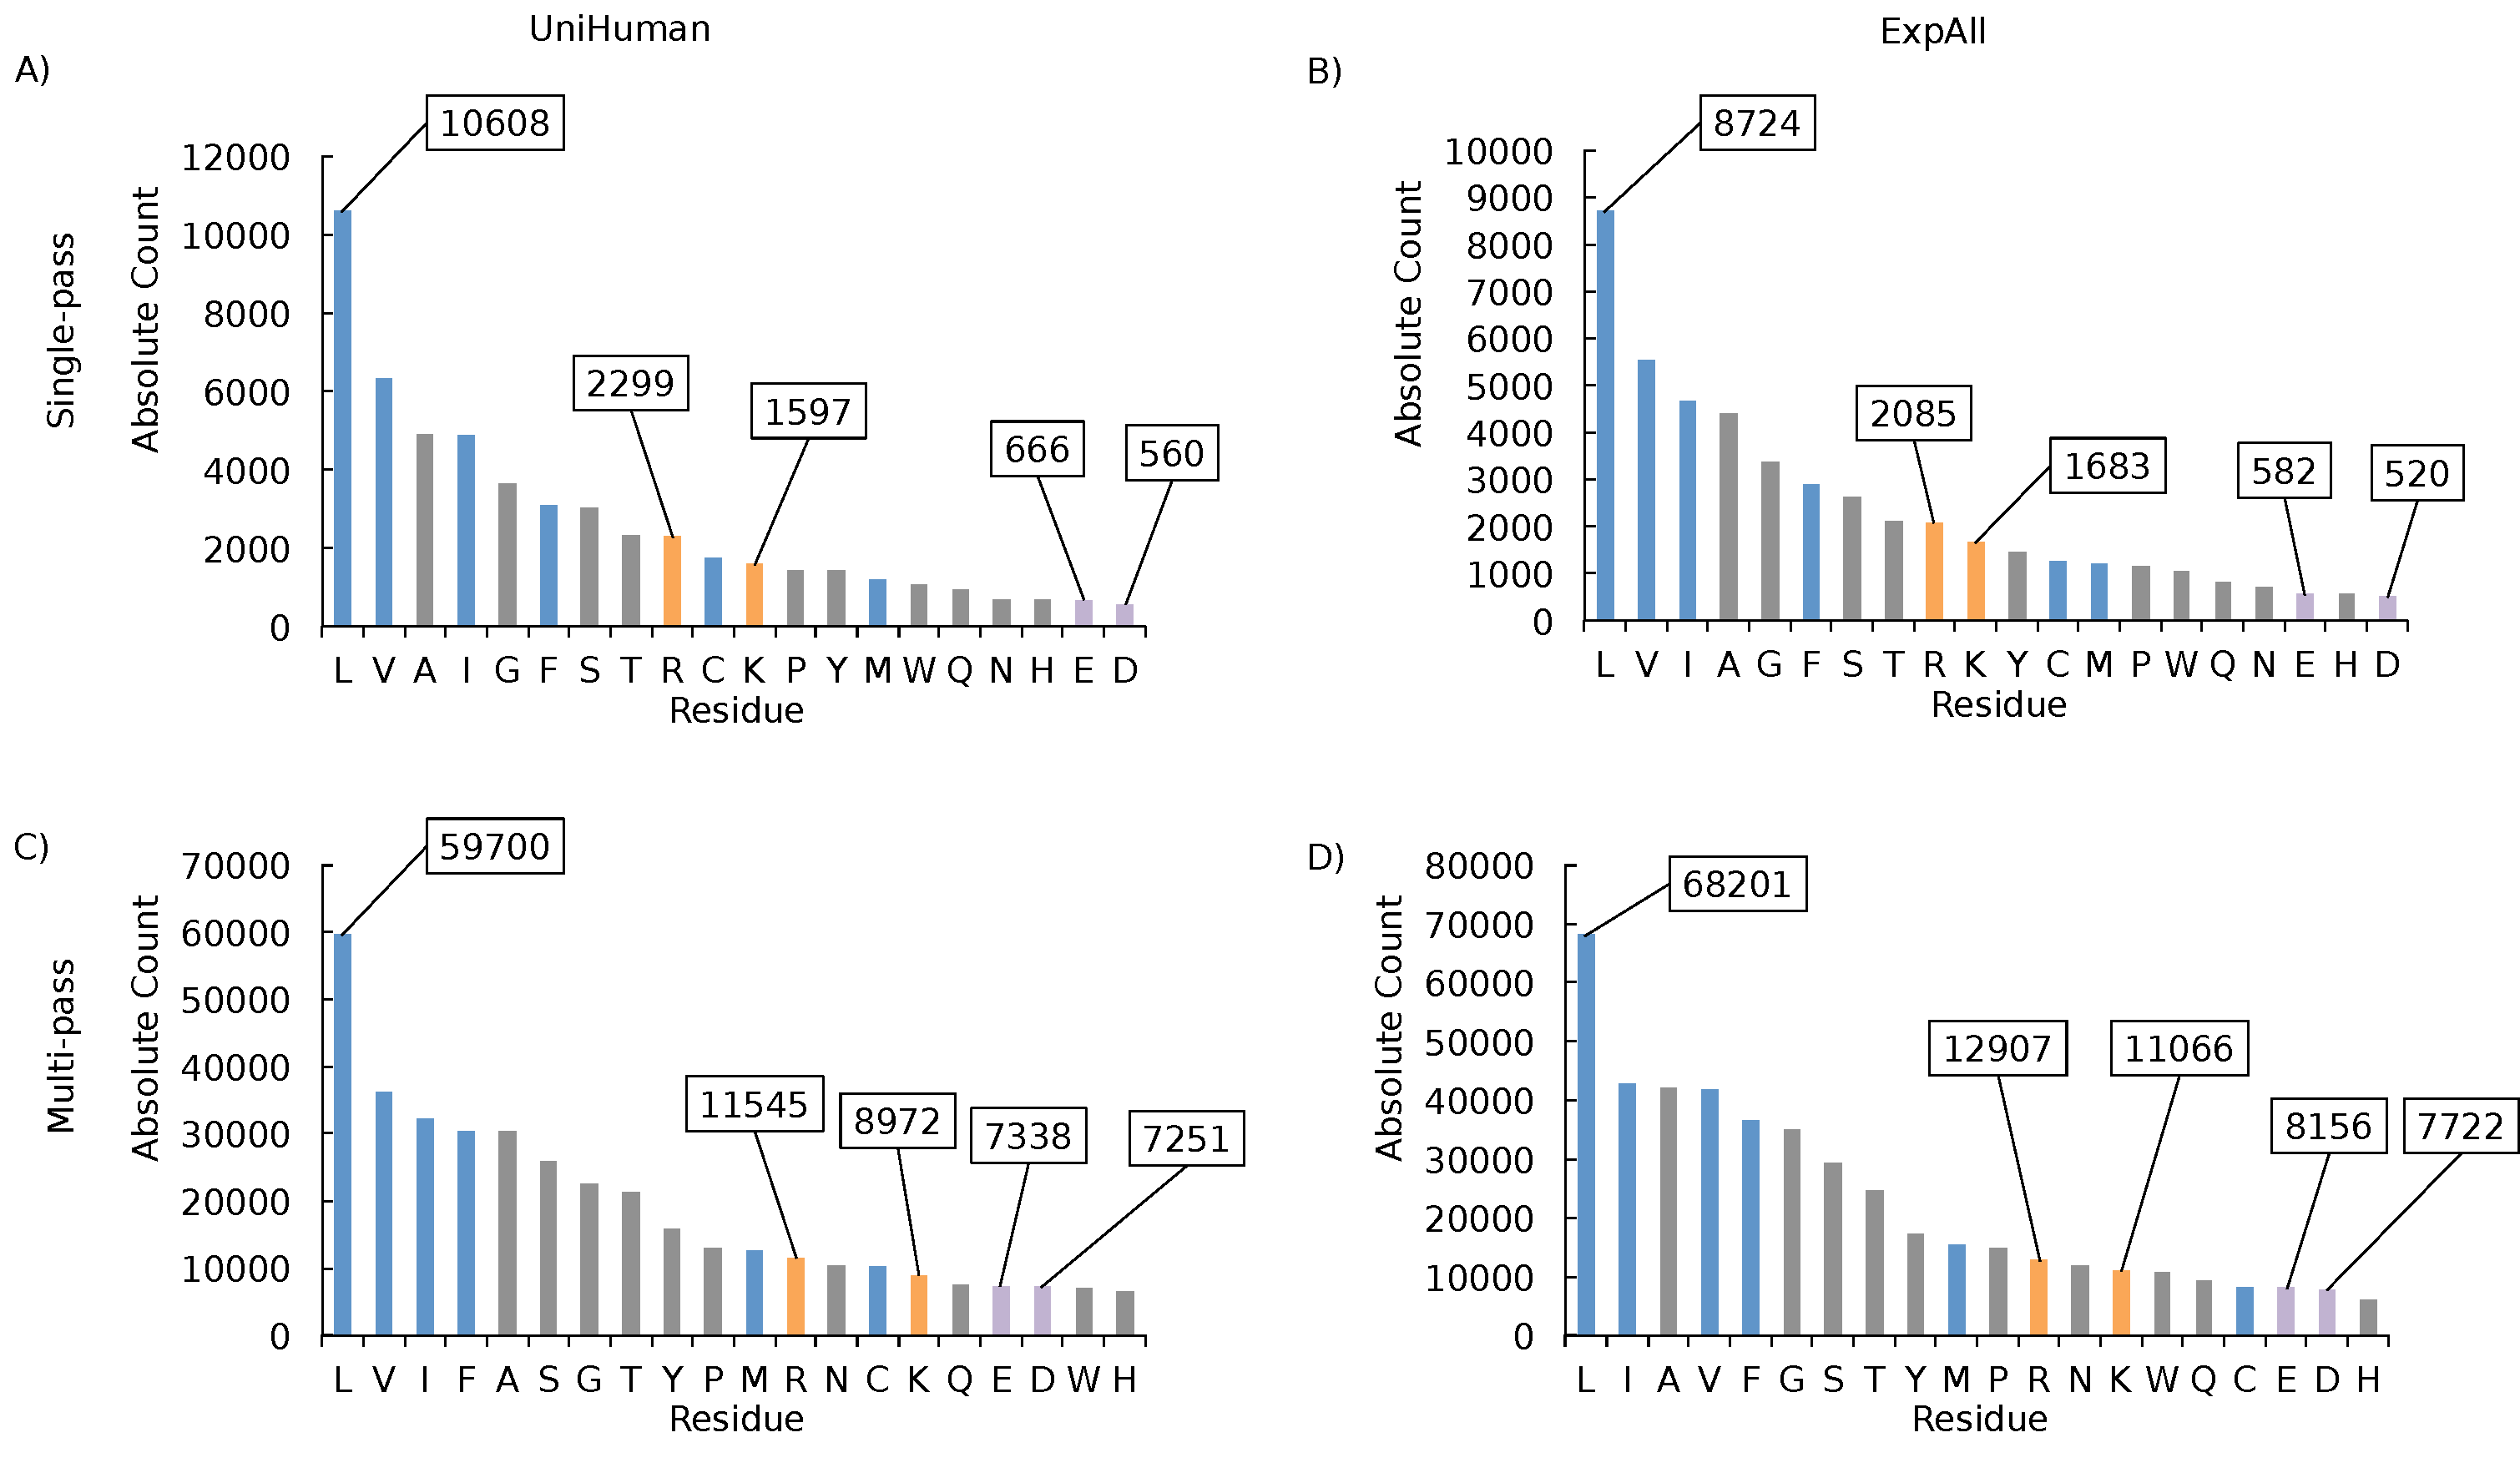
\includegraphics[width=1\textwidth]{NNI_chapter/amino_acid_distribution}
\captionof{figure}[Negatively charged amino acids are amongst the rarest residues in~\gls{tmh}s and $\pm$5 flanking residues.] {\textbf{Negatively charged amino acids are amongst the rarest residues in~\gls{tmh}s and $\pm$5 flanking residues.}Bar charts of the abundance of each amino acid type in the~\gls{tmh}s with flank lengths of the accompanying $\pm$5 residues from the (a) UniHuman single-pass proteins, (b) ExpAll single-pass proteins, (c) UniHuman multi-pass proteins, and (d) ExpAll multi-pass proteins.
Amino acid types on the horizontal axis are listed in descending count.
The bars were coloured according to categorisations of hydrophobic, neutral and hydrophilic types according to the free energy of insertion biological scale~\cite{Hessa2005}.
Grey represents hydrophilic amino acids that were found to have a positive $\Delta$G app, and blue represents hydrophobic residues with a negative $\Delta$G app, purple denotes negative residues and positive residues are coloured in orange.
The abundances of key residues are labelled.}

\label{fig:amino_acid_distribution}
\end{figure}

The effect is most pronounced in single-pass~\gls{tmp}s (Figure~\ref{fig:amino_acid_distribution}).
There are only 666 glutamates (just 1.24\% of all residues) and 560 aspartates (1.05\% respectively) among the total set of 53238 residues comprised in 1705~\gls{tmh}s and their flanks.
Within just the~\gls{tmh} regions, there are 71 glutamates (0.20\% of all residues in~\gls{tmh}s and flanks) and 58 aspartates (0.16\% respectively).
This cannot be an artefact of UniProt~\gls{tmh} assignments since this feature is repeated in ExpAll.
There are only 582 glutamates (1.22\%) and 520 aspartates (1.09\%) among the 47568 residues involved.
Within the~\gls{tmh} itself, there are 64 glutamates (0.19\%) and 69 aspartates (0.21\%).
In both cases, the negatively charged residues represent the ultimate end of the distribution.
To note, acidic residues are rare even compared to positively charged residues which are about 3--4 times more frequent.
On a much smaller dataset of single-spanning~\gls{tmp}, Nakashima \textit{et al.}
~\cite{Nakashima1992} made similar compositional studies.
To compare, they found 0.94\% glutamate and 0.94\% aspartate within just the~\gls{tmh} region (values very similar to ours from~\gls{tmh}s with small flanks; apparently, they used more outwardly defined~\gls{tmh} boundaries) but the content of each glutamate and aspartate within the extracellular or cytoplasmic domains is larger by an order of magnitude, between 5.26\% and 9.34\%.
These latter values tend to be even higher than the average glutamate and aspartate composition throughout the protein database (5--6\%~\cite{Nakashima1992}).

In the case of multi-pass~\gls{tmp}s (Figure~\ref{fig:amino_acid_distribution}), glutamates and aspartates are still very rare in~\gls{tmh}s and their $\pm$5 residue flanks (1.94\% and 1.92\% from the total of 377207 in the case of UniHuman respectively, 1.79\% and 1.70\% from the total of 454700 in the case of ExpAll).
Yet, their occurrence is similar to those of histidine and tryptophan and, notably, acidic residues are only about $\sim$1.5 times less frequent than positively charged residues.
The observation that acidic residues are more suppressed in single-pass~\gls{tmh}s compared with the case of multi-pass~\gls{tmh}s is statistically significant.
In Table \ref{table:acidicresiduesarerare}, the acidic residues are counted in the helices (excluding flanking regions) belonging to either multi-pass or single-pass helices.
Indeed, single-pass helices appear to tolerate negative charge to a far lesser extent than multi-pass helices as the data in the top two rows of Table \ref{table:acidicresiduesarerare} indicates (for datasets UniHuman and ExpAll).
The trend is strictly observed throughout sub-cellular localisations (rows 3--5 in Table \ref{table:acidicresiduesarerare}) and taxa (rows 6--10).
Statistical significance (P≤0.001) is found in all but six cases.
These are UniEcoli (D+E, D, E), UniArch (D+E, E) and UniFungi (E).
The problem is, most likely, that the respective datasets are quite small.
Notably, the difference between single- and multi-pass~\gls{tmh}s is greatest in UniPM\@; here,~\gls{tmh}s from multi-pass proteins have on average 0.400 negative residues per helix, whereas single-pass~\gls{tmh}s contained just 0.039 (P=3.86e-28).

\subsection{Amino acid residue distribution analysis reveals a ``negative-not-inside/negative-outside'' signal in single-pass~\gls{tmh} segments}

The rarity of negatively charged residues is a complicating issue when studying their distribution along the sequence positions of~\gls{tmh}s and their flanks.
For UniHuman and ExpAll , we plotted absolute abundance of aspartic acid, glutamic acid, lysine, arginine, and leucine at each position (i.e., it scales as the equivalent fraction in the total composition of the alignment column) (Figure~\ref{fig:single_pass_charge_distribution}).
To note, the known preference of positively charged residues towards the cytoplasmic side is nevertheless evident.
Yet, it becomes apparent that any bias in the occurrence of the much rarer acidic residues is overshadowed by fluctuations in the highly abundant residues such as leucine.

\begin{figure}[p]
\centering
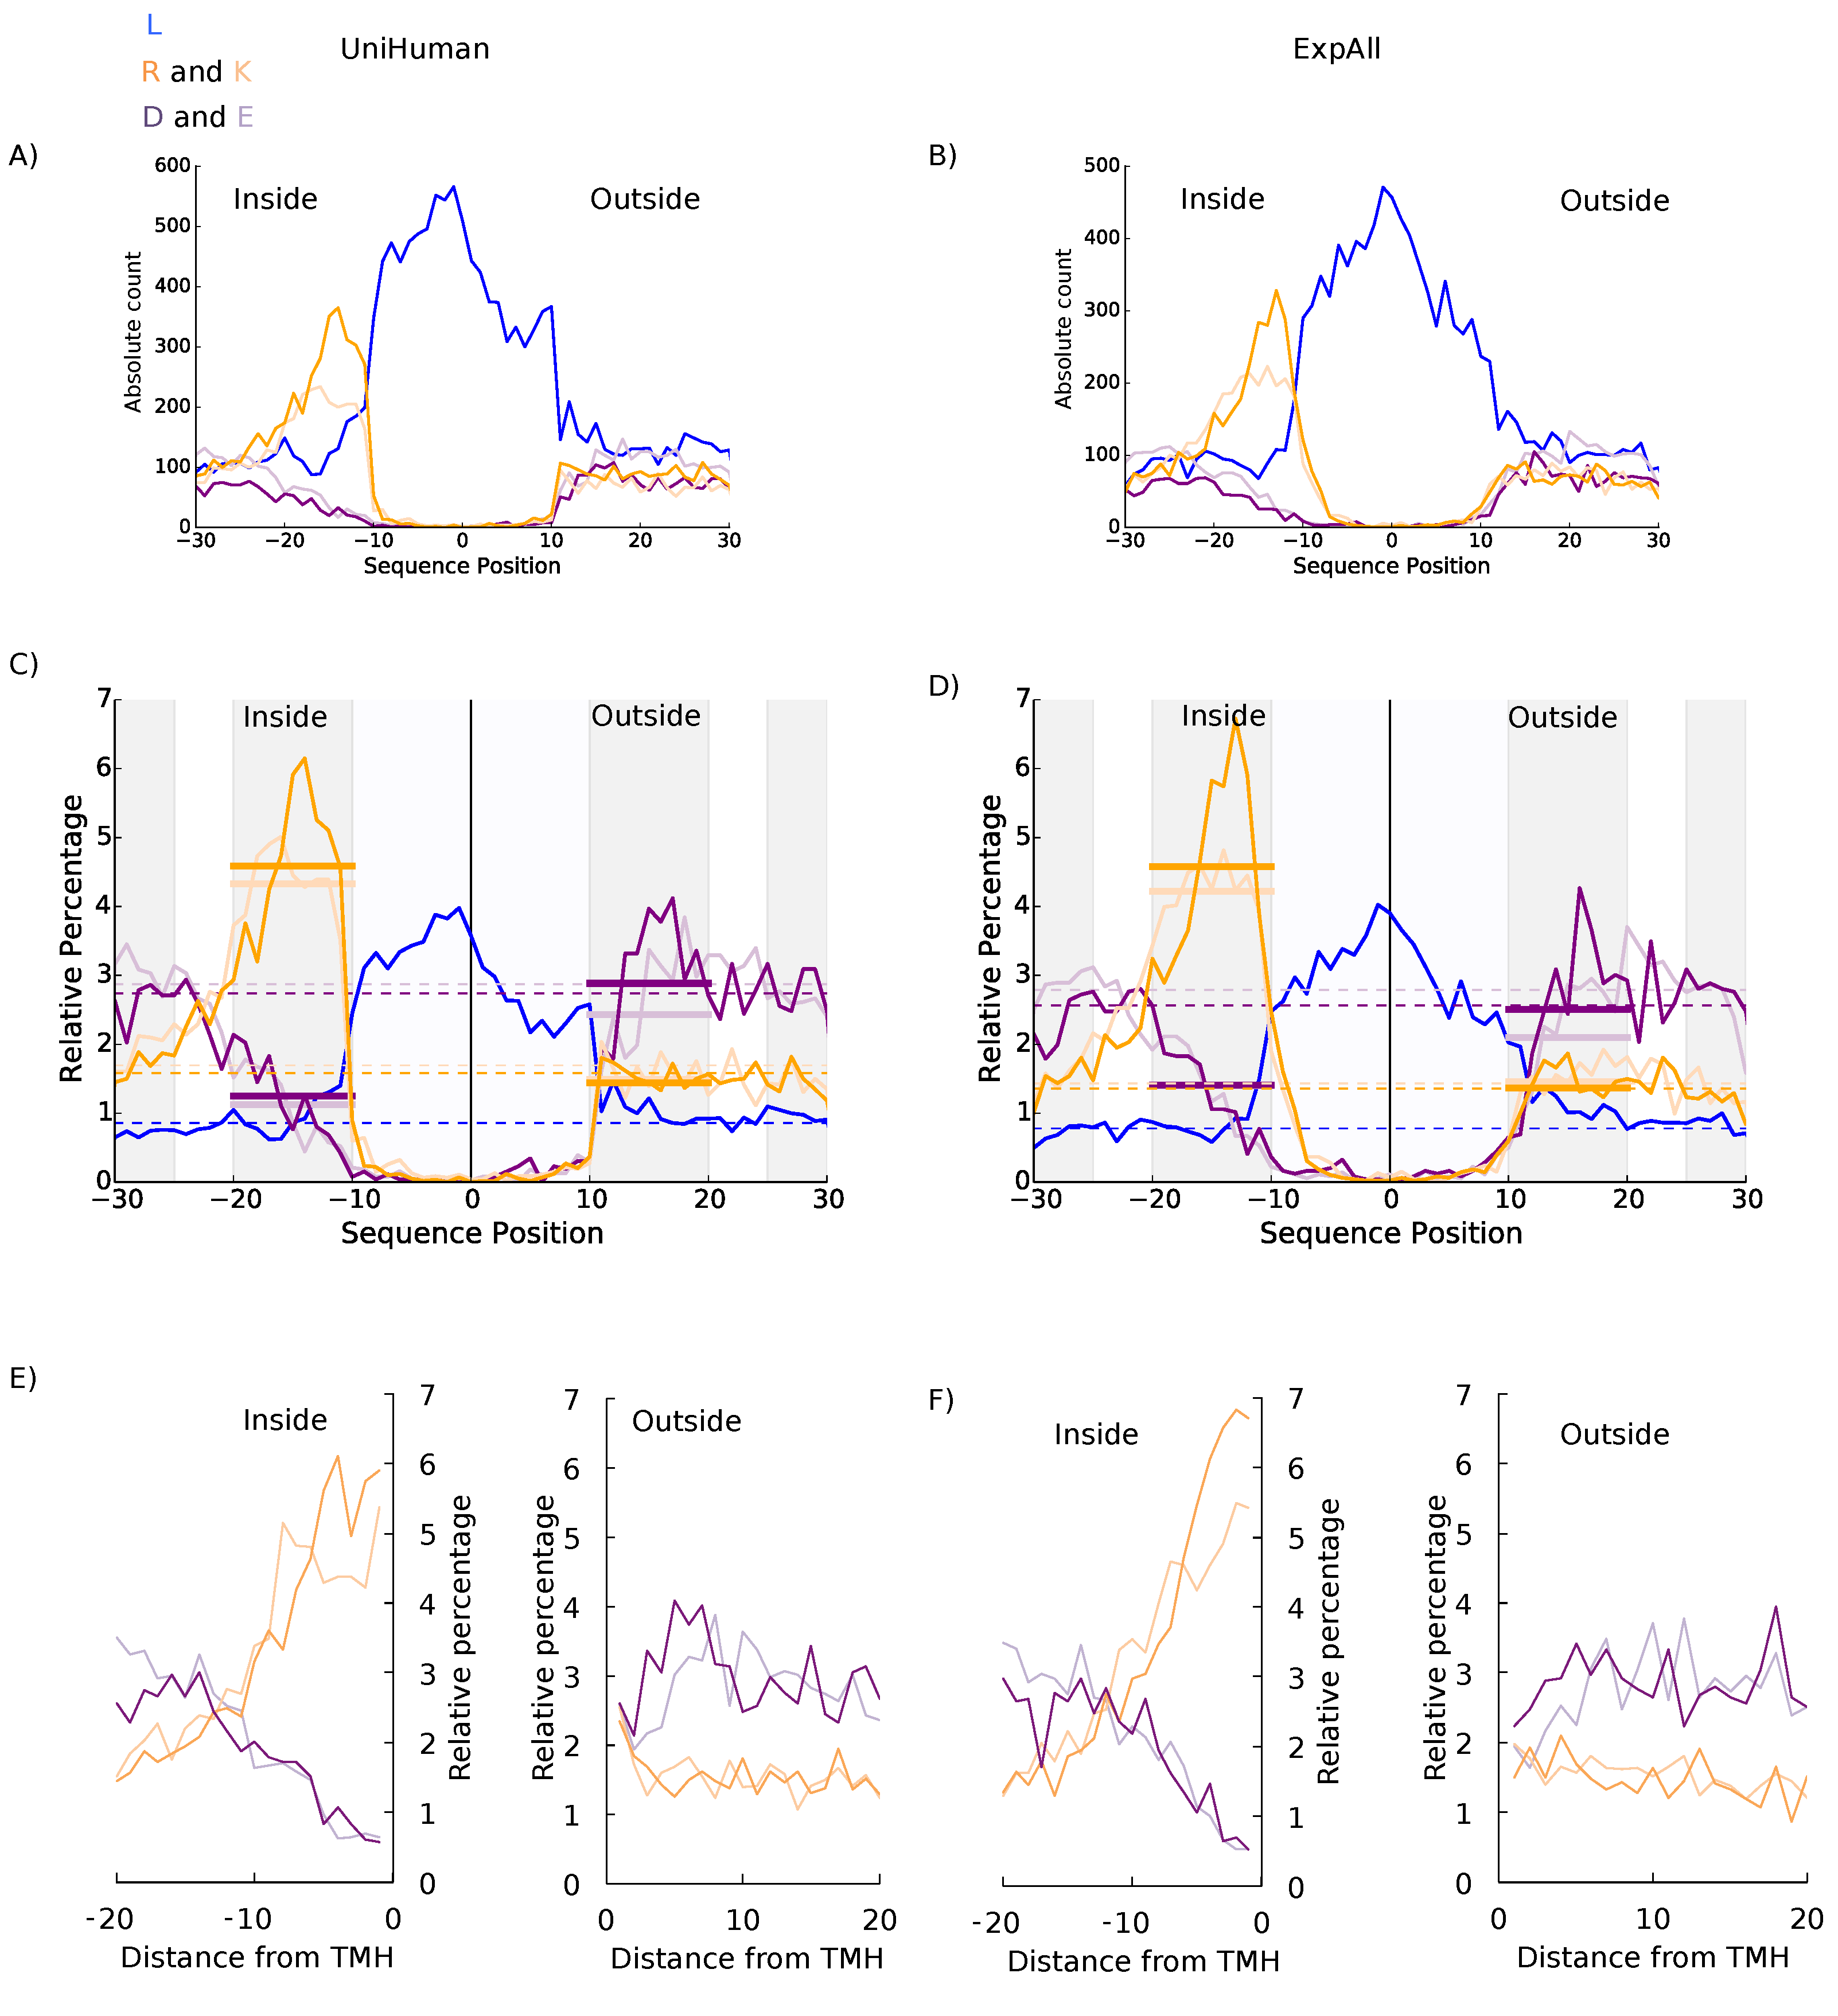
\includegraphics[width=1\textwidth]{NNI_chapter/single_pass_charge_distribution}
\captionof{figure}[Relative percentage normalisation reveals a negative-outside bias in~\gls{tmh}s from single-pass protein datasets.]{\textbf{Relative percentage normalisation reveals a negative-outside bias in~\gls{tmh}s from single-pass protein datasets.} All flank sizes were set at up to $\pm$20 residues.
We acknowledge that all values, besides the averaged values, are discrete, and connecting lines are illustrative only.
On the horizontal axes (a–d) are the distances in residues from the centre of the~\gls{tmh}, with the negative numbers extending towards the cytoplasmic space.
For (e) and (f), the horizontal axis represents the residue count from the membrane boundary with negative counts into the cytoplasmic space.
Leucine, the most abundant non-polar residue in~\gls{tmh}s, is in blue.
Arginine and lysine are shown in dark and light orange respectively.
Aspartic and glutamic acid are showing in dark and light purple respectively.
(a) and (b) On the vertical axis is the absolute abundance of residues in~\gls{tmh}s from single-pass proteins from (a) UniHuman and (b) ExpAll.
Note that no clear trend can be seen in the negative residue distribution compared to the positive-inside signal and the leucine abundance throughout the~\gls{tmh}.
c and d On the vertical axis is the relative percentage at each position for~\gls{tmh}s from single-pass proteins from (c) UniHuman and (d) ExpAll.
The dashed lines show the estimation of the background level of residues with respect to the colour; an average of the relative percentage values between positions 25 to 30 and –30 to –25.
The thick bars show the averages on the inner (positions –20 to –10) and outer (positions 10 to 20) flanks coloured to the respective amino acid type.
Note a visible suppression of acidic residues on the inside flank when compared to the outside flank in single-pass proteins when normalising according to the relative percentage.
(e) and (f) The relative distribution of flanks defined by the databases with the distance from the~\gls{tmh} boundary on the horizontal axis.
The inside and outside flanks are shown in separate subplots.
The colouring is the same as in (a) and (b).}


\label{fig:single_pass_charge_distribution}
\end{figure}

The trends become clearer if the occurrence of specific residues is normalised with the total number of residues of the given amino acid type in the dataset observed in the sequence region studied as shown for UniHuman and for ExpAll in Figure~\ref{fig:single_pass_charge_distribution}.
For comparison, we indicated background residue occurrences (dashed lines calculated as averages for positions -25 to -30 and 25 to 30).
The respective average occurrences in the inside and outside flanks (calculated from an average of the values at positions -20 to -10 and 10 to 20 respectively) are shown with wide lines.

The ``positive-inside rule'' becomes even more evident in this normalisation: Whereas the occurrence of positively charged residues is about the background level at the outside flank, it is about two to three times higher both for the UniHuman and the ExpAll datasets at the inside flank.
To note, the background level was found to be 1.7\% (lysine) and 1.6\% (arginine) in UniHuman and 1.4\% (lysine and arginine) in ExpAll.
The inside flank average is 4.3\% (lysine) and 4.6\% (arginine) in UniHuman and 4.2\% (lysine) and 4.6\% (arginine) in ExpAll.
The outside flank is similar to the background noise levels: about 1.4\% (lysine) and 1.5\% (arginine) in UniHuman and about 1.5\% (lysine) and 1.4\% (arginine) in ExpAll.

Most interestingly, a ``negative‑inside depletion'' trend for the negatively charged residues is apparent from the distribution bias.
The inside flank averages for glutamic acid were 1.1\% and 1.4\% in UniHuman and ExpAll respectively; for aspartic acid, 1.2\% and 1.4\% in UniHuman and ExpAll respectively.
Meanwhile, the outside flanks for aspartic acid and glutamic acid occurrences were measured at 2.9\% and 2.4\% respectively in UniHuman and, in ExpAll, these values for aspartic acid and glutamic acid were found to be 2.5\% and 2.1\% respectively.
Against the background level of aspartic acid (2.8\% and 2.9\% in UniHuman) and glutamic acid (2.6\% and 2.9\% in ExpAll), the inside flank averages were found to be about 2--3 times lower than the background level while the outside flank averages were comparable to the background level (Figure~\ref{fig:single_pass_charge_distribution}).
Taken together, this indicates a clear suppression of negatively charged residues at the inside flank of single-pass~\gls{tmh}s and a possible trend for negatively charged residues occurring preferentially at the outside flank.
This is not an effect of the flank definition selection since the trend remains the same when using the database-defined flanks without the context of the~\gls{tmh} (Figure~\ref{fig:single_pass_charge_distribution}).
For UniHuman, the negative charge expectancy on the inside flank doesn’t reach above 2\% until position -10 (D) and position -11 (E), whereas, on the outside flank, both D and E start $>$2\%.
The same can be seen in ExpAll where negative residues reach above 2\% only as far from the membrane boundary as at position -9 (D) and position -7 (E) on the inside but exceed 2\% beginning with position 1 (D) and 3 (E) on the outside (Figure~\ref{fig:single_pass_charge_distribution}).

The observation of negative charge suppression at the inside flank, herein the ``negative-inside depletion'' rule, is statistically significant throughout most datasets in this study.
The inside-outside bias was counted using the~\gls{kw} test comparing the occurrence of acidic residues within 10 residues of each~\gls{tmh} inside and outside the~\gls{tmh} (Table~\ref{table:negativeskewsinglepass}).
We studied both the database-reported flanks as well as those obtained from central alignment of~\gls{tmh}s (see Methods).
The null hypothesis (no difference between the two flanks) could be confidently rejected in all cases (P-value$<$0.001 except for UniBacilli), the sign of the H-statistic (\gls{kw}) indicating suppression at the inside and/or preference for the outside flank (except for UniArch).
Most importantly, acidic residues were found to be distributed with bias in ExpAll (P-value$<$3.47e-58) and in UniHuman (P-value=1.13e-93).
Whereas with UniBacilli, the problem is most likely the dataset size, the exception of UniArch, for which we observe a strong negative inside rule, is more puzzling and indicates biophysical differences of their plasma-membrane.

% Table generated by Excel2LaTeX from sheet 'Sheet1'
\begin{table}[htbp!]

    \centering
    \captionof{table}[Statistical significances for negative charge distribution skew on either side of the membrane in single-pass~\gls{tmh}s]{\textbf{Statistical significances for negative charge distribution skew on either side of the membrane in single-pass~\gls{tmh}s}The “Helices” column refers to the total~\gls{tmh}s contained in each dataset (ExpALL,~\gls{tmh}s from TOPDB~\cite{Dobson2015}; UniHuman, human representative proteome; UniER, human endoplasmic reticulum representative proteome; UniGolgi, human Golgi representative proteome; UniPM, human plasma membrane representative proteome; UniCress, Arabidopsis thaliana (mouse-ear cress) representative proteome; UniFungi, fungal representative proteome; UniBacilli, Bacilli class representative proteome; UniEcoli, Escherichia coli representative proteome; UniArch, Archaea representative proteome; see Methods for details).
In the ``Database-defined flanks'' column, the ``Negative residues'' column refers to the total number of negative residues found in the $\pm$10 flanking residues on either side of the~\gls{tmh} and does not include residues found in the helix itself.
In the ``Flanks after central alignment'' column, the ``Negative residues'' column refers to the total number of negative residues found in the –20 to –10 residues and the +10 to +20 residues from the centrally aligned residues of the~\gls{tmh}.
Unlike the other tables, the global averages are derived from the $\pm$20 datasets.
The~\gls{kw} scores were calculated for negative residues by comparing the number of negatively charged residues that were within the 10 inside residues and the 10 outside residues in either case}
    \resizebox{\textwidth}{!}{
     \begin{tabular}{p{5em}lllllllll}
     \toprule
     \multicolumn{2}{p{10em}}{\textbf{Single-pass}} & \multicolumn{4}{p{20em}}{\textbf{Database-defined flanks}} & \multicolumn{4}{p{20em}}{\textbf{Flanks after central alignment}} \\
     \midrule
     \multirow{2}[4]{*}{\textbf{Data-set}} & \multicolumn{1}{c}{\multirow{2}[4]{*}{\textbf{Helices}}} & \multicolumn{2}{p{10em}}{\textbf{Negative residues}} & \multicolumn{1}{c}{\multirow{2}[4]{*}{\textbf{H statistic}}} & \multicolumn{1}{c}{\multirow{2}[4]{*}{\textbf{P value}}} & \multicolumn{2}{p{10em}}{\textbf{Negative residues}} & \multicolumn{1}{c}{\multirow{2}[4]{*}{\textbf{H statistic}}} & \multicolumn{1}{c}{\multirow{2}[4]{*}{\textbf{P value}}} \\
 \cmidrule{3-4}\cmidrule{7-8}    \multicolumn{1}{c}{} &       & \multicolumn{1}{p{5em}}{\textbf{Inside}} & \multicolumn{1}{p{5em}}{\textbf{Outside}} &       &       & \multicolumn{1}{p{5em}}{\textbf{Inside}} & \multicolumn{1}{p{5em}}{\textbf{Outside}} &       &  \\
     \midrule
     ExpAll & 1544  & 848   & 1648  & 258.59 & 3.47E-58 & 735   & 1541  & 262.29 & 5.44E-59 \\
     \midrule
     UniHuman & 1705  & 780   & 1922  & 421.53 & 1.13E-93 & 652   & 1865  & 501.86 & 3.74E-111 \\
     \midrule
     UniER & 132   & 78    & 156   & 23.76 & 1.09E-06 & 76    & 150   & 21.62 & 3.33E-06 \\
     \midrule
     UniGolgi & 206   & 60    & 240   & 104.45 & 1.61E-24 & 54    & 239   & 107.18 & 4.06E-25 \\
     \midrule
     UniPM & 493   & 197   & 578   & 177.68 & 1.56E-40 & 161   & 569   & 215.18 & 1.02E-48 \\
     \midrule
     UniCress & 632   & 314   & 450   & 18.23 & 1.96E-05 & 231   & 444   & 55.8  & 8.01E-14 \\
     \midrule
     UniFungi & 729   & 449   & 631   & 28.15 & 1.12E-07 & 413   & 627   & 38.08 & 6.79E-10 \\
     \midrule
     UniBacilli & 124   & 90    & 113   & 3.73  & 5.35E-02 & 86    & 106   & 2.53  & 1.12E-01 \\
     \midrule
     UniEcoli & 54    & 32    & 77    & 17.24 & 3.30E-05 & 30    & 74    & 14.74 & 1.24E-04 \\
     \midrule
     UniArch & 48    & 113   & 8     & 49.66 & 1.83E-12 & 96    & 7     & 45.62 & 1.43E-11 \\
     \bottomrule
     \end{tabular}}%
     \label{table:negativeskewsinglepass}

    \end{table}%

\subsection{Amino acid residue distribution analysis reveals a general negative charge bias signal in outside flank of multi-pass~\gls{tmh} segments --- the negative outside enrichment rule}

As a result of the rarity of negatively charged residues, any distribution bias is difficult to be recognised in the plot showing the total abundance (or alignment column composition) of residues in multi-pass~\gls{tmh}s and their flanks from UniHuman and ExpAll (Figure~\ref{fig:multi_pass_charge_distribution}).
Yet, as with single-pass helices, the dominant general leucine enrichment, as well as positive inside signal, can be identified with certainty.
When the residue occurrence is normalised by the total occurrence of this residue type in the sequence regions studied (shown as a relative percentage of at each position for multi-pass helices from UniHuman and ExpAll  in Figure~\ref{fig:multi_pass_charge_distribution}), the bias in the distribution of any type of charged residues becomes visible.

\begin{figure}[!p]
\centering
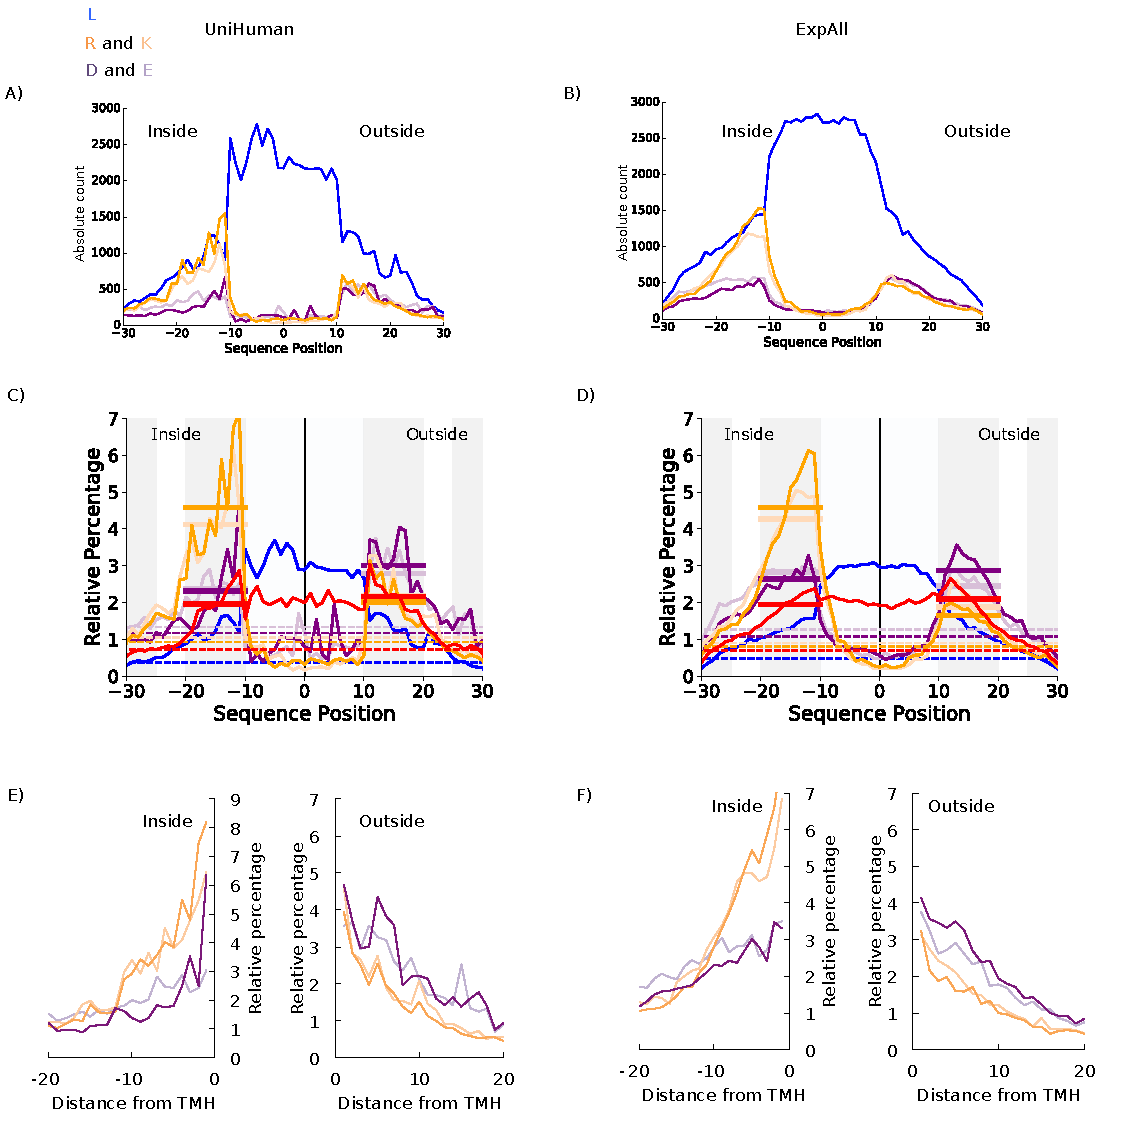
\includegraphics[width=1\textwidth]{NNI_chapter/multi_pass_charge_distribution}
\captionof{figure}[Negative-outside bias is very subtle in~\gls{tmh}s from multi-pass proteins.]{\textbf{Negative-outside bias is very subtle in~\gls{tmh}s from multi-pass proteins.}The meaning for the horizontal axis is the same as in Figure~\ref{fig:single_pass_charge_distribution}, with the negative sequence position numbers extending towards the cytoplasmic space.
Leucine is in blue.
Arginine and lysine are shown in dark and light orange respectively.
Aspartic and glutamic acid are shown in dark and light purple respectively.
All flank sizes were set at up to $\pm$20 residues.
(a) and (b) On the vertical axes are the absolute abundances of residues from~\gls{tmh}s of multi-pass proteins from (a) UniHuman and (b) ExpAll.
c and d On the vertical axes are the relative percentages at each position for~\gls{tmh}s from multi-pass proteins from (c) UniHuman and (d) ExpAll.
As in Figure~\ref{fig:single_pass_charge_distribution}(c) and (d), the dashed lines show the estimation of the background level of residues with respect to the colour, and the thick bars show the averages on the inner and outer flanks coloured to the respective amino acid type.
e and f The relative distribution of flanks defined by the databases with the distance from the~\gls{tmh} boundary on the horizontal axis for both the inside and outside flanks.
The colouring is the same as in (a) and (b).}

\label{fig:multi_pass_charge_distribution}
\end{figure}

With regard to the positive-inside preference, positively charged residues have a background value of 2.0\% for arginine and 2.2\% for lysine in UniHuman, and 1.7\% for arginine and 1.9\% for lysine in ExpAll.
At the inside flank, this rises to 4.6\% for arginine and 4.1\% for lysine in UniHuman and 4.6\% for arginine and 4.2\% for lysine in ExpAll.
The mean net charge at each position was calculated for multi-pass and single-pass datasets from UniHuman and ExpAll (Figure \ref{fig:net_charge}).
The positive inside rule clearly becomes visible as the net charge has a positive skew approximately between residues -10 and -25.
What is noteworthy is that the peaks found for single-pass helices were almost three times greater than those of multi-pass helices.
For single-pass~\gls{tmh}s, the peak is +0.30 at position -15 in UniHuman and +0.31 at position -14 in ExpAll, whereas~\gls{tmh}s from multi-pass proteins had lower peaks of +0.15 at position -13 in UniHuman and +0.10 at position -14 in ExpAll.
Thus, there is a positive charge bias towards the cytoplasmic side; yet, it is much weaker for multi-pass than for single-pass~\gls{tmh}s.

\begin{figure}[!ht]
\centering
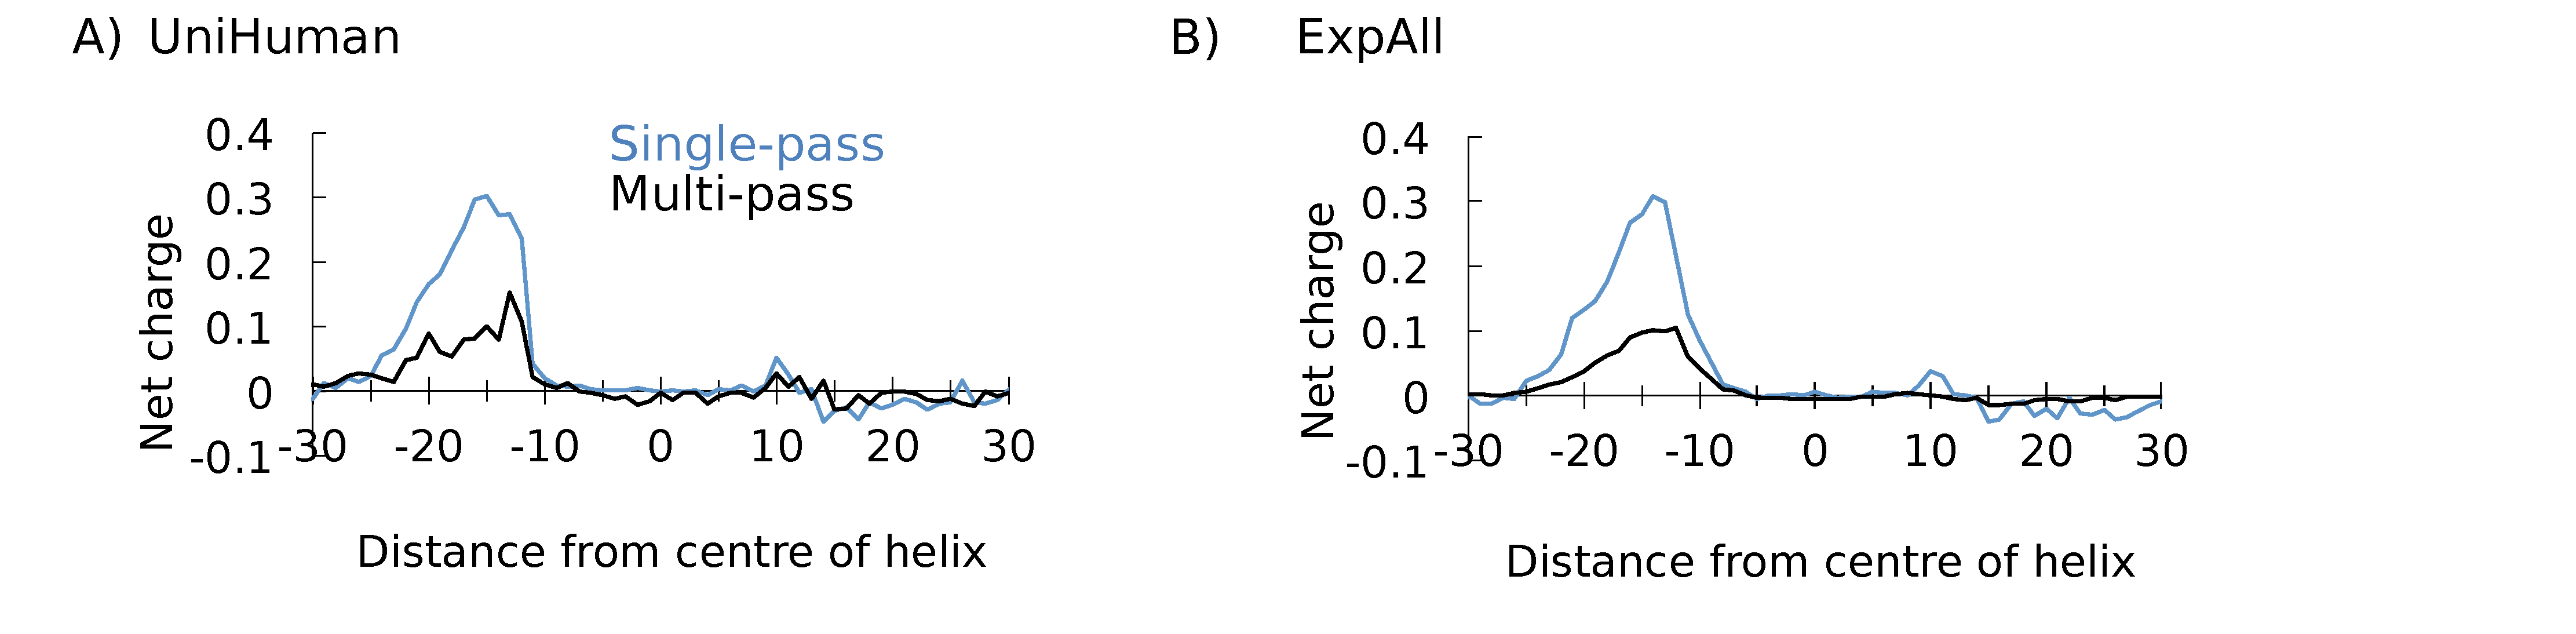
\includegraphics[width=1\textwidth]{NNI_chapter/net_charge}
\captionof{figure}[The net charge across multi-pass and single-pass~\gls{tmh}s shows a stronger positive inside charge in single-pass~\gls{tmh}s than multi-pass~\gls{tmh}s.]{\textbf{The net charge across multi-pass and single-pass~\gls{tmh}s shows a stronger positive inside charge in single-pass~\gls{tmh}s than multi-pass~\gls{tmh}s.}
The net charge per~\gls{tmh} plotted at each position; the positive-inside rule is stronger in~\gls{tmh}s from single-pass proteins than~\gls{tmh}s from multi-pass proteins.
The net charge was calculated at each position as described in the Methods section for the (A) UniHuman and (B) ExpAll datasets.
Net charge for~\gls{tmh}s from multi-pass proteins is shown in black, and the profile of~\gls{tmh}s from single-pass proteins is drawn in blue.}

\label{fig:net_charge}
\end{figure}

Notably, a ``negative outside enrichment'' trend also can be seen from the distribution of the negatively charged residues, though with some effort (Table 3) as the effect is also weaker than in the case of single-pass~\gls{tmh}s.
We studied the flanks under four conditions: (i) database-defined flanks without overlap between neighbouring~\gls{tmh}s, (ii) flanks after central alignment of~\gls{tmh}s without flank overlap, (iii) database-defined flanks but allowing overlap of flanks shared among neighbouring~\gls{tmh}s, (iv) same as condition (ii) but only the subset of cases where there is at least half of the required flank length at either side of the~\gls{tmh}.
In UniHuman as calculated under condition (i), aspartic acid is lower on the inside flank (2.3\%) than on the outside flank (3.0\%).
Glutamic acid is also lower at the inside flank (2.4\%) than the 2.8\% on the outside flank (Figure~\ref{fig:multi_pass_charge_distribution}C).
Slight variations in defining the membrane boundary point do not influence the trend (compare figures~\ref{fig:multi_pass_charge_distribution}C and~\ref{fig:multi_pass_charge_distribution}E).
We find that, in all studied conditions, the UniHuman dataset delivers statistical significances (P-values: (i) 6.10e-34, (ii) 5.43e-41, (iii) 3.00e-57, (iv) 5.60e-41) strongly supporting negative charge bias (inside suppression/outside preference; see Table~\ref{tab:multipassstats}).

% Table generated by Excel2LaTeX from sheet 'Sheet1'

\begin{table}[htbp]
  \centering
  \captionof{table}[Statistical significances for negative charge distribution skew on either side of the membrane in multi-pass~\gls{tmh}s]{\textbf{Statistical significances for negative charge distribution skew on either side of the membrane in multi-pass~\gls{tmh}s}
The ``Helices'' column refers to the total~\gls{tmh}s contained in each dataset (ExpALL,~\gls{tmh} from TOPDB~\cite{Dobson2015}; UniHuman, human representative proteome; UniER, human endoplasmic reticulum representative proteome; UniGolgi, human Golgi representative proteome; UniPM, human plasma membrane representative proteome; UniCress, Arabidopsis thaliana (mouse-ear cress) representative proteome, UniFungi, fungal representative proteome; UniBacilli, Bacilli class representative proteome; UniEcoli, Escherichia coli representative proteome; UniArch, Archaea representative proteome; see Methods for details).
In (A) the ``Database-defined flanks'' and in (B) the ``Database-defined viable* flanks'' and the ``Overlapping flanks'' columns, the ``Negative residues'' column refers to the total number of negative residues found in the $\pm$10 flanking residues on either side of the~\gls{tmh} and does not include residues found in the~\gls{tmh} itself.
(A) In the ``Flanks after central alignment'' column, the ``Negative residues'' column refers to the total number of negative residues found in the –20 to –10 residues and the +10 to +20 residues from the centrally aligned residues with a maximum database defined flank length of 20 residues.
The total number of proteins is given in the IDs column.
The ``Helices'' column contains the total number of~\gls{tmh}s in the dataset (n), the average number of~\gls{tmh}s per protein in that population ($\mu$) and the standard deviation of that average ($\sigma$).
The~\gls{kw} scores were calculated for negative residues by comparing the number of negatively charged residues that were within 10 residues inside and 10 residues outside the~\gls{tmh}.

*Here, ``viable'' indicates that in each~\gls{tmh} used for both flanks either side of the~\gls{tmh} has a flank length of at least half the maximum allowed flank length, in this case 10 (the viable length is 5)}

\resizebox{\textwidth}{!}{(A)
    \begin{tabular}{ p{5em} l l l l l l l l l l l l }
    \toprule
    \multicolumn{5}{ p{25em} }{Multi-pass} & \multicolumn{4}{p{20em} }{Database-defined flanks} & \multicolumn{4}{p{20em} }{Flanks after central alignment} \\
    \midrule
    \multirow{2}[4]{*}{Data-set} & \multicolumn{1}{l }{\multirow{2}[4]{*}{IDs}} & \multicolumn{3}{p{15em} }{Helices} & \multicolumn{2}{p{10em} }{Negative residues} & \multicolumn{1}{l }{\multirow{2}[4]{*}{H statistic}} & \multicolumn{1}{l }{\multirow{2}[4]{*}{P value}} & \multicolumn{2}{p{10em} }{Negative residues} & \multicolumn{1}{l }{\multirow{2}[4]{*}{H statistic}} & \multicolumn{1}{l }{\multirow{2}[4]{*}{P value}} \\
    \cmidrule{3-7}\cmidrule{10-11}    \multicolumn{1}{ l }{} &       & \multicolumn{1}{p{5em} }{\textit{n}} & \multicolumn{1}{p{5em} }{$\mu$} & \multicolumn{1}{p{5em} }{$\sigma$} & \multicolumn{1}{p{5em} }{Inside} & \multicolumn{1}{p{5em} }{Outside} &       &       & \multicolumn{1}{p{5em} }{Inside} & \multicolumn{1}{p{5em} }{Outside} &       &  \\
    \midrule
    ExpAll & 2205  & 15,563 & 7.07  & 3.95  & 9709  & 9598  & 0.04  & 8.43E-01 & 9648  & 9659  & 0.35  & 5.56E-01 \\
    \midrule
    UniHuman & 1789  & 12,353 & 6.93  & 3.2   & 7196  & 9164  & 147.5 & 6.10E-34 & 6740  & 8968  & 179.77 & 5.43E-41 \\
    \midrule
    UniER & 155   & 898   & 5.85  & 3.2   & 630   & 584   & 0.44  & 5.08E-01 & 578   & 576   & 0.03  & 8.58E-01 \\
    \midrule
    UniGolgi & 61    & 383   & 6.28  & 2.97  & 274   & 261   & 0.02  & 8.75E-01 & 266   & 259   & 0.09  & 7.65E-01 \\
    \midrule
    UniPM & 427   & 3079  & 7.22  & 3.3   & 1945  & 2499  & 47.98 & 4.30E-12 & 1791  & 2440  & 64.42 & 1.01E-15 \\
    \midrule
    UniCress & 507   & 3823  & 7.55  & 3.32  & 2567  & 2426  & 0.73  & 3.93E-01 & 2398  & 2433  & 1.11  & 2.93E-01 \\
    \midrule
    UniFungi & 1338  & 8685  & 6.5   & 3.75  & 5560  & 5266  & 5.83  & 1.57E-02 & 5140  & 5214  & 0     & 9.62E-01 \\
    \midrule
    UniBacilli & 140   & 822   & 5.94  & 3.98  & 470   & 468   & 0.07  & 7.92E-01 & 450   & 471   & 0.92  & 3.38E-01 \\
    \midrule
    UniEcoli & 529   & 3888  & 7.39  & 3.76  & 1990  & 1902  & 0.26  & 6.07E-01 & 1875  & 1887  & 0.18  & 6.71E-01 \\
    \midrule
    UniArch & 59    & 327   & 5.97  & 2.73  & 245   & 175   & 7.98  & 4.72E-03 & 235   & 181   & 7.08  & 7.81E-03 \\
    \bottomrule
    \end{tabular}
    }
    \\

    \resizebox{\textwidth}{!}{(B)
    % Table generated by Excel2LaTeX from sheet 'Sheet1'
    \begin{tabular}{ p{5em} l l l l l l l l llll }
    \toprule
    Multi-pass & \multicolumn{4}{p{20em} }{Overlapping flanks} & \multicolumn{8}{p{40em} }{Database-defined viable* flanks} \\
    \midrule
    \multirow{2}[4]{*}{Data-set} & \multicolumn{2}{p{10em} }{Negative residues} & \multicolumn{1}{l }{\multirow{2}[4]{*}{H statistic}} & \multicolumn{1}{l }{\multirow{2}[4]{*}{P value}} & \multicolumn{1}{l }{\multirow{2}[4]{*}{\textit{N}}} & \multicolumn{2}{p{10em} }{Negative residues} & \multicolumn{1}{l }{\multirow{2}[4]{*}{H statistic}} & \multicolumn{4}{l }{\multirow{2}[4]{*}{P value}} \\
\cmidrule{2-3}\cmidrule{7-8}    \multicolumn{1}{ l }{} & \multicolumn{1}{p{5em} }{Inside} & \multicolumn{1}{p{5em} }{Outside} &       &       &       & \multicolumn{1}{p{5em} }{Inside} & \multicolumn{1}{p{5em} }{Outside} &       & \multicolumn{4}{l }{} \\
    \midrule
    ExpAll & 11,969 & 12,615 & 22.54 & 2.05E-06 & 8808  & 6082  & 6916  & 59.93 & \multicolumn{4}{l }{9.81E-15} \\
    \midrule
    UniHuman & 8645  & 11,181 & 254.3 & 3.00E-57 & 8183  & 5169  & 6915  & 179.71 & \multicolumn{4}{l }{5.60E-41} \\
    \midrule
    UniER & 750   & 763   & 1.16  & 2.81E-01 & 516   & 398   & 441   & 3.16  & \multicolumn{4}{l }{7.55E-02} \\
    \midrule
    UniGolgi & 333   & 369   & 7.12  & 7.64E-03 & 195   & 162   & 186   & 3     & \multicolumn{4}{l }{8.30E-02} \\
    \midrule
    UniPM & 2319  & 3107  & 99.68 & 1.79E-23 & 1977  & 1343  & 1960  & 98.63 & \multicolumn{4}{l }{3.05E-23} \\
    \midrule
    UniCress & 3142  & 3298  & 9.21  & 2.41E-03 & 2110  & 1626  & 1741  & 6.4   & \multicolumn{4}{l }{1.14E-02} \\
    \midrule
    UniFungi & 6724  & 6814  & 0.46  & 4.96E-01 & 4581  & 3340  & 3411  & 0.41  & \multicolumn{4}{l }{5.22E-01} \\
    \midrule
    UniBacilli & 585   & 636   & 2.65  & 1.04E-01 & 382   & 230   & 306   & 12.73 & \multicolumn{4}{l }{3.61E-04} \\
    \midrule
    UniEcoli & 2574  & 2800  & 17.88 & 2.35E-05 & 1596  & 951   & 1114  & 16.57 & \multicolumn{4}{l }{4.69E-05} \\
    \midrule
    UniArch & 342   & 248   & 14.67 & 1.28E-04 & 132   & 120   & 104   & 0.28  & \multicolumn{4}{l }{5.97E-01} \\
    \bottomrule
    \end{tabular}%
    }
  \label{tab:multipassstats}
\end{table}

Surprisingly, the result could not straightforwardly be repeated with the considerably smaller ExpAll.
Under condition (i), we find with ExpAll that aspartic acid has a background level of 1.0\%, an average of 2.6\% on the inside flank, and of 2.9\% on the outside flank but glutamic acid’s background is 1.2\% but 2.8\% on the inside flank and 2.5\% on the outside flank.
Statistical tests do not support finding a negative charge bias in conditions (i) and (ii).
Apparently, the problem is~\gls{tmh}s having no or almost no flanks at one of the sides.
Statistical significance for the negative charge bias is detected as soon as this problem is dealt with – either by allowing extension of flanks overlap among neighbouring~\gls{tmh}s as in condition (iii) or by kicking out examples without proper flank lengths from the dataset as in condition (iv).
The respective P-values are 2.05e-6 and 9.81e-15 respectively.

The issues we had with ExpAll raised the question that, maybe, sequence redundancy in the UniHuman set could have played a role.
Therefore, we repeated all calculations but with UniRef50 instead of UniRef90 for mapping into sequence clusters (see Methods section for detail).
We were surprised to see that harsher sequence redundancy requirements do not affect the outcome of the statistical tests in any major way.
For the conditions (i)- (iv), we computed the following P-values: (i) 1.31e-28 (5940 negatively residues inside versus 7492 outside), (ii) 1.38e-36 (5516 versus 7320), (iii) 5.60e-53 (7089 versus 9233) and (iv) 4.18e-41 (4232 versus 5730).

So, the amplifying effect of some subsets in the overall dataset on the statistical test that might be caused by allowing overlapping flanks (condition (iii)) is not the major factor leading to the negative charge skew.
Similarly, the trend is also not caused by sequence redundancy.
Thus, we have learned that the negative charge bias does also exist in multi-pass~\gls{tmp}s but under the conditions that there are sufficiently long loops between~\gls{tmh}s.
Bluntly said: no loops equals to no charge bias.
As soon as the loops reach some critical length, there are differences between single-pass and multi-pass~\gls{tmh}s with regard to occurrence and distribution of negative charges and the inside-suppression/outside-enrichment negative charge bias appears.
Not only are there more negative charges within the multi-pass~\gls{tmh} itself (in fact, negative charges are almost not tolerated in single-pass~\gls{tmh}s; see Table \ref{table:acidicresiduesarerare}), but also, there is a much stronger negative outside skew in the~\gls{tmh}s of single-pass proteins than those of multi-pass proteins.

\subsection{Further significant sequence differences between single-pass and multi-pass helices: distribution of tryptophan, tyrosine, proline and cysteine}

Amino acid residue profiles along the~\gls{tm} segment and its flanks differ between single- and multi-pass~\gls{tmh}s also in other aspects.
The relative percentages of all amino acid types (normalisation by the total amount of that residue type in the sequence segment) from single-pass helices of the UniHuman (Figure \ref{fig:comp_heatmaps}A; from 1705~\gls{tmh}s with flanks having 68571 residues) and ExpAll (Figure \ref{fig:comp_heatmaps}B; from 1544~\gls{tmh}s with flanks having 60200 residues) were plotted as a heat-map.
The amino acid types were listed on the Y axis according to Kyte \& Doolittle hydrophobicity~\cite{Kyte1982} in descending order.

\begin{figure}[p]
\centering
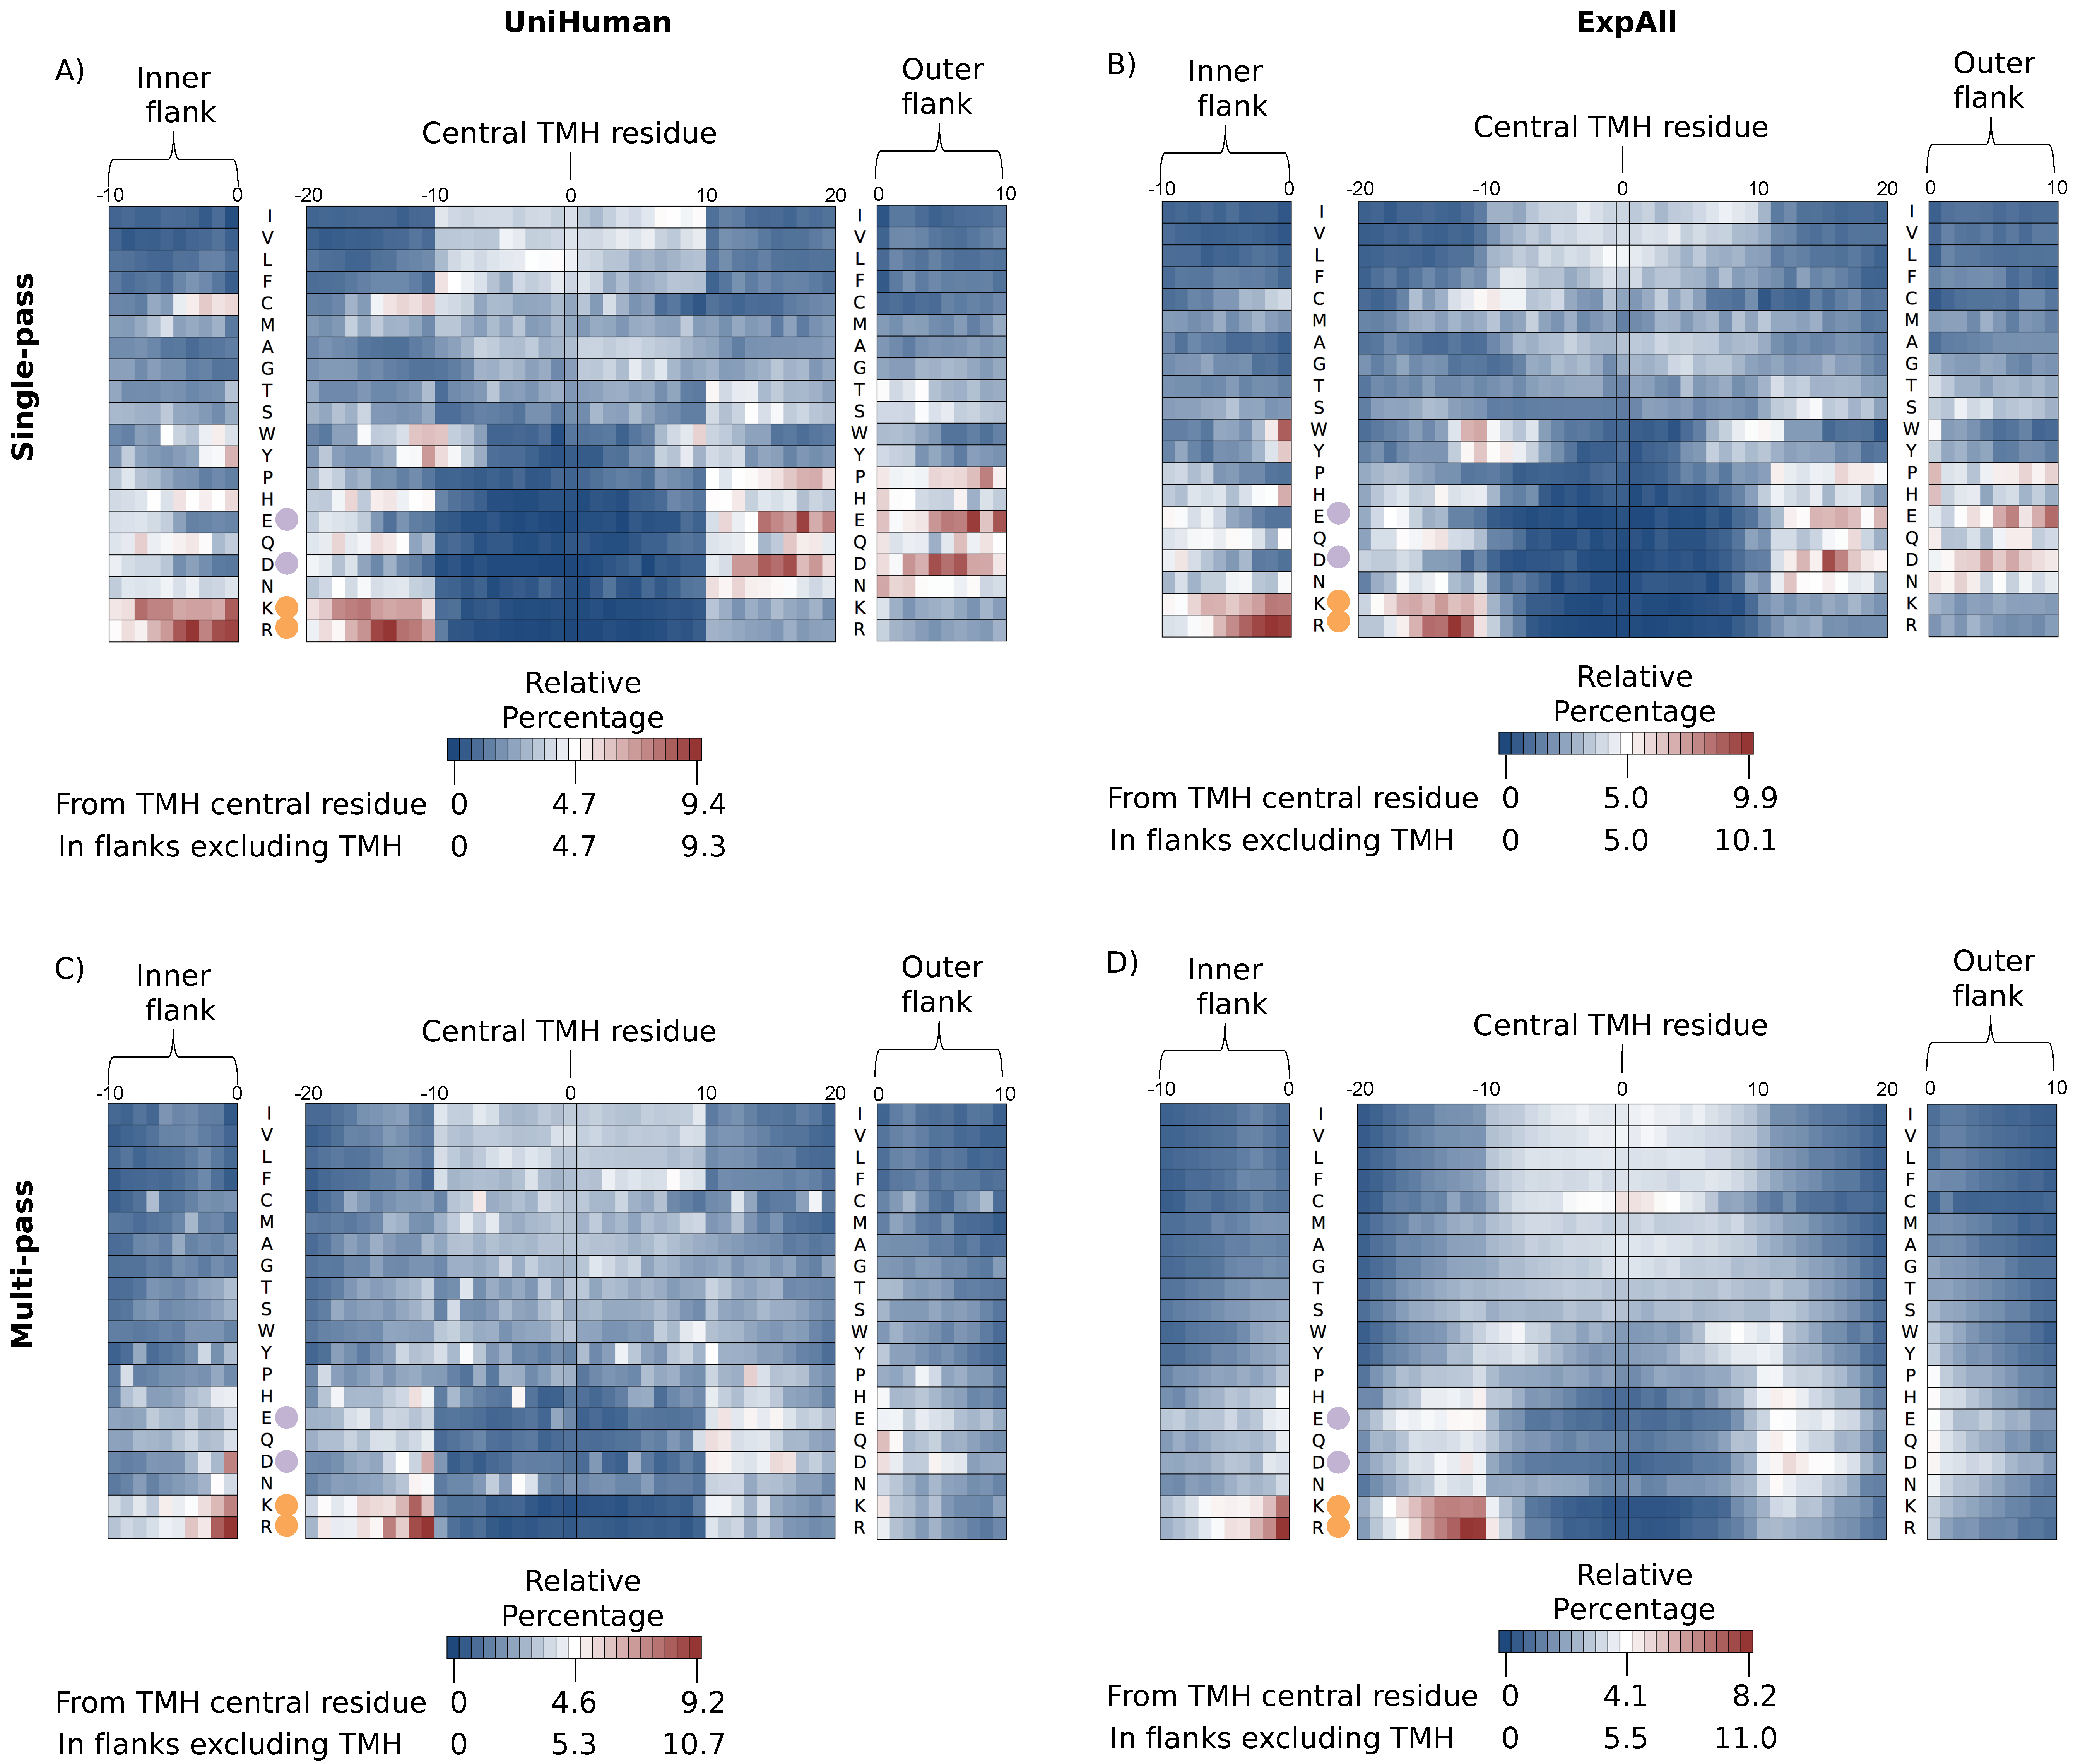
\includegraphics[width=1\textwidth]{NNI_chapter/comp_heatmaps}
\captionof{figure}[Relative percentage heat-maps from predictive and experimental datasets corroborate residue distribution differences between~\gls{tmh}s from single-pass and multi-pass proteins.]{\textbf{Relative percentage heat-maps from predictive and experimental datasets corroborate residue distribution differences between~\gls{tmh}s from single-pass and multi-pass proteins.}
The residue position aligned to the centre of the~\gls{tmh} is on the horizontal axis, and the residue type is on the vertical axis.
Amino acid types are listed in order of decreasing hydrophobicity according to the Kyte and Doolittle scale [52].
The flank lengths in the~\gls{tmh} segments were restricted to up to $\pm$10 residues.
The scales for each heat-map are shown beneath the respective subfigure.
The darkest blue represents 0\% distribution, whilst the darkest red represents the maximum relative percentage distribution that is denoted by the keys in each subfigure, with white being 50\% between ``cold'' and ``hot''.
The central~\gls{tmh} subplots extend from the central~\gls{tmh} residue, whereas the inner and outer flank subplots use the database-defined~\gls{tmh} boundary and extend from that position.
a~\gls{tmh}s from the single-pass UniHuman dataset.
b Single-pass protein~\gls{tmh}s from the ExpAll dataset.
c~\gls{tmh}s from the proteins of the multi-pass UniHuman dataset.
d~\gls{tmh}s from ExpAll multi-pass proteins.
The general consistency in relative distributions of every residue type between single-pass and multi-pass of either dataset including flank/\gls{tmh} boundary selection allows us to infer biological conclusions from these distributions that are independent of methodological biases used to gather the sequences.
The only residue that displays drastically differently between the datasets is cysteine in multi-pass~\gls{tmh}s only.
The most striking differences in distributions between residues from~\gls{tmh}s of single-pass and multi-pass proteins include a more defined Y and W clustering at the flanks, a suppression of E and D on the inside flank, a suppression of P on the inside flank and a topological bias for C favouring the inside flank.}

\label{fig:comp_heatmaps}
\end{figure}

In accordance with expectations, enrichment for hydrophobic residues in the~\gls{tmh}, for the positively charged residues on the inside flank as well as a distribution the negative distribution bias was found in both datasets.
Additionally, the inside interfacial region showed consistent enrichment hotspots for tryptophan (e.g., 7.1\% at position -11 in ExpAll, 6.2\% at position -10 in UniHuman with flanks after central~\gls{tmh} alignment) and tyrosine (6.4\% at -11 in ExpAll, 7.1\% at -11 in UniHuman), and some preference can also be seen for the outer interfacial region (\textit{e.g.}, 5.2\% at position 11 for tryptophan in ExpAll, and 5.8\% at position 10 for tryptophan in UniHuman) albeit the ``hot'' cluster of the outer flank covers fewer positions than that of the inner flank.
Further, there is an apparent bias of cysteine on the inner flank and interfacial region (e.g., 5.5\% at position -10 in ExpAll, 5.9\% at position -11 in UniHuman), and a depression in the outer interfacial region and flank (up to a minimum of 0.3\% in both ExpAll and UniHuman).
Proline appears to have a depression signal on the outer flank.
Note that, in a similar way to Figures \ref{fig:single_pass_charge_distribution} and \ref{fig:multi_pass_charge_distribution}, the distributions of the flanks derived from centrally aligned~\gls{tmh}s are corroborated by the distributions from the database defined~\gls{tmh} boundary flanks (see outside bands in Figures \ref{fig:comp_heatmaps}A-D).

A similar heatmap was generated for UniHuman multi-pass (Figure \ref{fig:comp_heatmaps}C; from 12353~\gls{tmh}s with flanks having 452708 residues)~\gls{tmh}s and ExpAll multi-pass (Figure \ref{fig:comp_heatmaps}D; from 15563~\gls{tmh}s with flanks having 535599 residues).
Whereas Figures \ref{fig:comp_heatmaps}A-C appear quite noisy, the plot for ExpAll multi-pass~\gls{tmh}s appears almost Gaussian-like smoothed, thus, indicating the quality of this dataset.
Tyrosine and tryptophan in the multi-pass case do not appear as enriched in the interfacial regions of single-pass~\gls{tmh}s from both UniHuman and ExpAll.
Prolines are only suppressed in the~\gls{tmh} itself and are not suppressed in the outer flank as in the single-pass case but, indeed, are tolerated if not slightly enriched in the flanks.

\subsection{Hydrophobicity and leucine distribution in~\gls{tmh}s in single- and multi-pass proteins}

Generally, we see in Figure \ref{fig:comp_heatmaps} that compositional biases appear more extreme in the single-pass case, particularly when it comes to polar and non-polar residues being more heavily suppressed and enriched.
To investigate this observation, we calculated the hydrophobicity at each sequence-position averaged over all~\gls{tmh}s considered (after having window-averaged over 3 residues for each~\gls{tmh}) using the Kyte \& Doolittle hydrophobicity scale~\cite{Kyte1982} (Figure~\ref{fig:hydrophobicity_single_multi}A) and validated using White and Wimley octanol-interface whole residue scale~\cite{White1999}, Hessa’s biological hydrophobicity scale~\cite{Hessa2005}, and the Eisenberg hydrophobic moment consensus scale~\cite{Eisenberg1984} (Supplementary Figure~\ref{fig:hydrophobicity_scale_comparison}).
The total set of~\gls{tmh}s was split into 15 sets of membrane-spanning proteins (1 set containing single-pass proteins, 13 sets each containing~\gls{tmh}s from 2-, 3-, 4-\ldots 14-\gls{tmp}s and another of~\gls{tmh}s from proteins with 15 or more~\gls{tmh}s).
In Figure~\ref{fig:hydrophobicity_single_multi}B, we show the P-value at each sequence position by comparing the respective values from multi-pass and single-pass~\gls{tmh}s using the 2-sample t-test (Figure \ref{fig:hydrophobicity_single_multi}B).
Strikingly, the inside flank of the single-pass~\gls{tmh}s is much more hydrophilic (e.g., see the Kyte \& Doolittle score=-1.3 at position -18) than that of multi-pass~\gls{tmh}s (P-value=5.64e-103 at position -14).
Most likely, the positive inside rule, along with the interfacial clustering of tryptophan and tyrosine, contribute to a strong polar inside flank in single-pass helices that is not present in multi-pass helices en masse.
Further, multi-pass~\gls{tmh}s cluster remarkably closely within the~\gls{tm} core; the respective hydrophobicity is apparently not dependent on the number of~\gls{tmh}s in a given multi-pass~\gls{tmp}.
On average, single-pass~\gls{tmh}s are more hydrophobic in the core than multi-pass~\gls{tmh}s (P-value$<$1.e-72 within positions -5…5 and P-value=5.92e-190 at position 0).
On the other hand, hydrophobicity differences between~\gls{tmh}s from single- and multi-pass proteins fade somewhat at the transition towards the flanks (P-value=1.85e-4 at position -10, and P-value=3.35e-31 at position 10).

\begin{figure}[!ht]
\centering
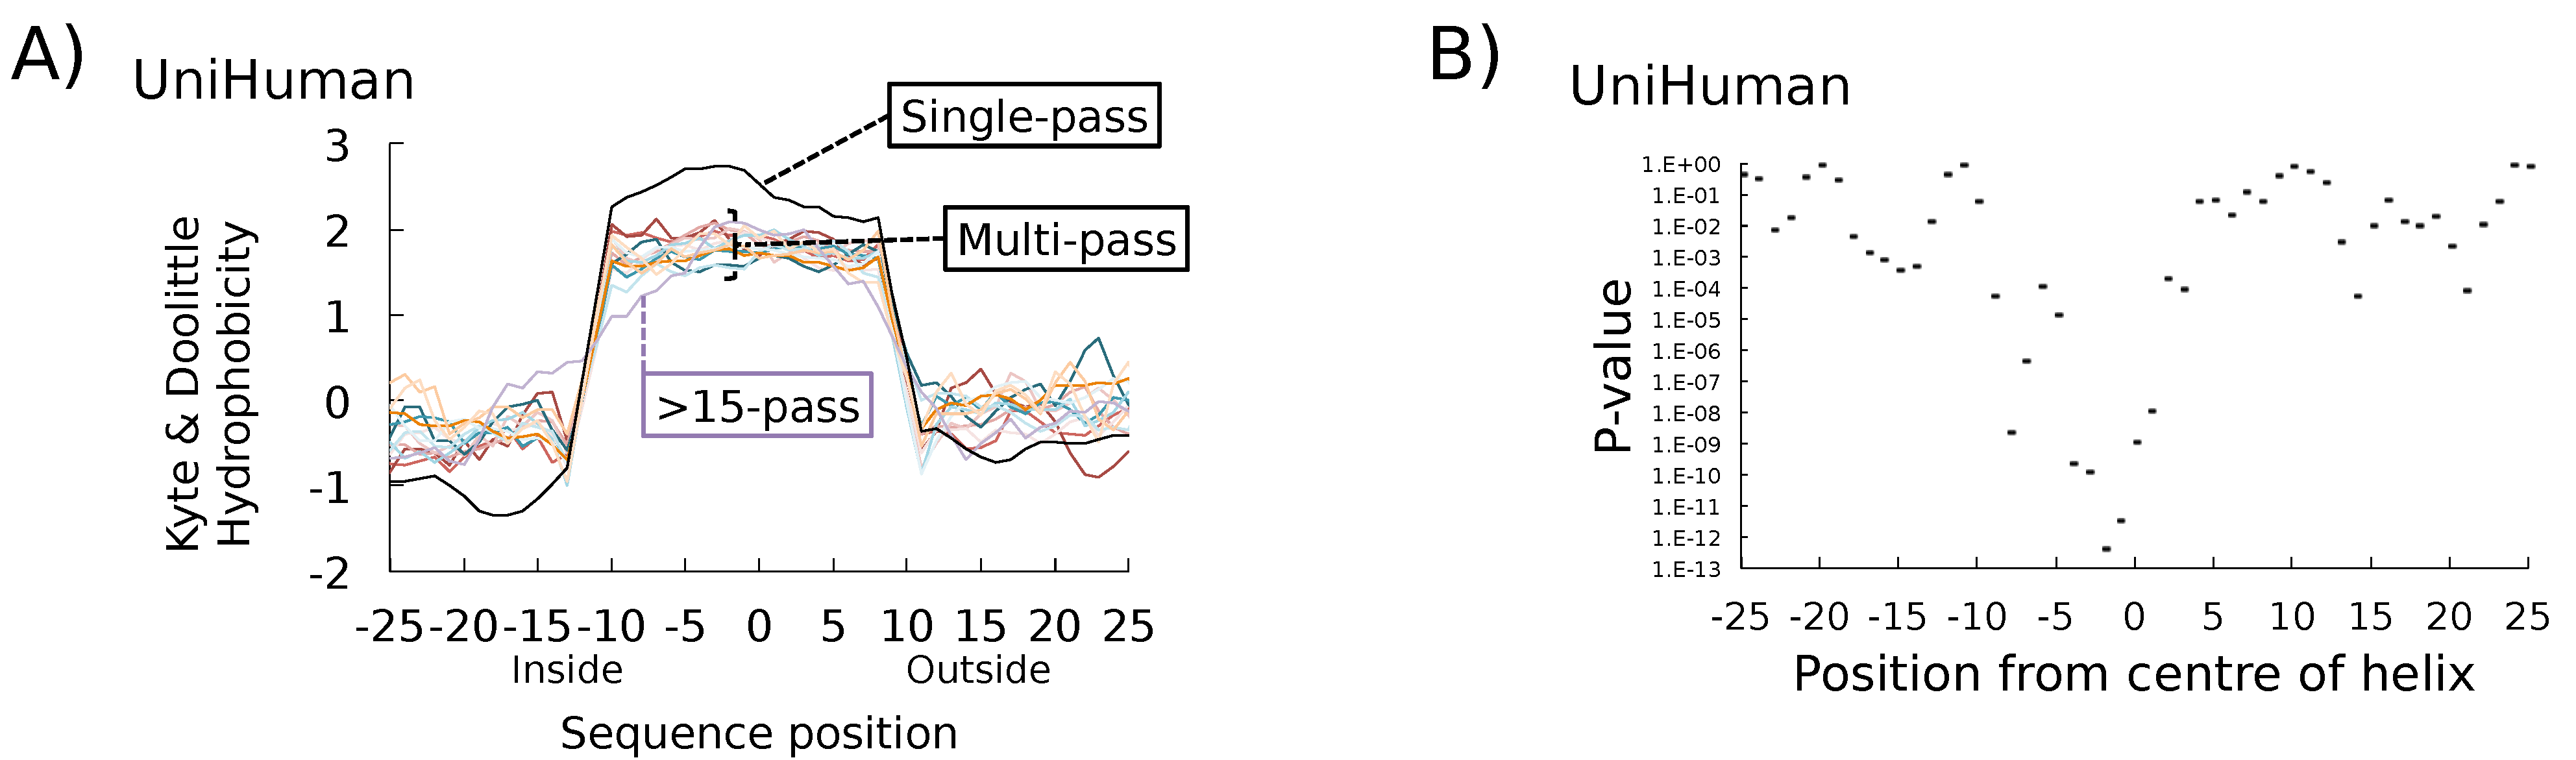
\includegraphics[width=1\textwidth]{NNI_chapter/hydrophobicity_single_multi}
\captionof{figure}[There is a difference in the hydrophobic profiles of~\gls{tmh}s from single-pass and multi-pass proteins.]{\textbf{There is a difference in the hydrophobic profiles of~\gls{tmh}s from single-pass and multi-pass proteins.}
 a The hydrophobicity of single-pass~\gls{tmh}s compared to multi-pass segments from the UniHuman dataset.
The Kyte and Doolittle scale of hydrophobicity~\cite{Kyte1982} was used with a window length of 3 to compare~\gls{tmh}s from proteins with different numbers of~\gls{tmh}s.
This scale is based on the water-vapour transfer of free energy and the interior-exterior distribution of individual amino acids.
The same datasets also had different scales applied (Figure~\ref{fig:hydrophobicity_scale_comparison}).
The vertical axis is the hydrophobicity score, whilst the horizontal axis is the position of the residue relative to the centre of the~\gls{tmh}, with negative values extending into the cytoplasm.
In black are the average hydrophobicity values of~\gls{tmh}s belonging to single-pass~\gls{tmh}s, whilst in other colours are the average hydrophobicity values of~\gls{tmh}s belonging to multi-pass proteins containing the same numbers of~\gls{tmh}s per protein.
In purple are the~\gls{tmh}s from proteins with more than 15~\gls{tmh}s per protein that do not share a typical multi-pass profile, perhaps due to their exceptional nature.
b The Kruskal-Wallis test (H statistic) was used to compare single-pass windowed hydrophobicity values with the average windowed hydrophobicity value of every~\gls{tmh} from multi-pass proteins at the same position.
The vertical axis is the logarithmic scale of the resultant P values.
We can much more readily reject the hypothesis that hydrophobicity is the same between~\gls{tmh}s from single-pass and multi-pass proteins in the core of the helix and the flanks than the interfacial regions, particularly at the inner leaflet due to leucine asymmetry ( Table~\ref{table:leucineskewstats})}

\label{fig:hydrophobicity_single_multi}
\end{figure}

\begin{figure}[!ht]
\centering
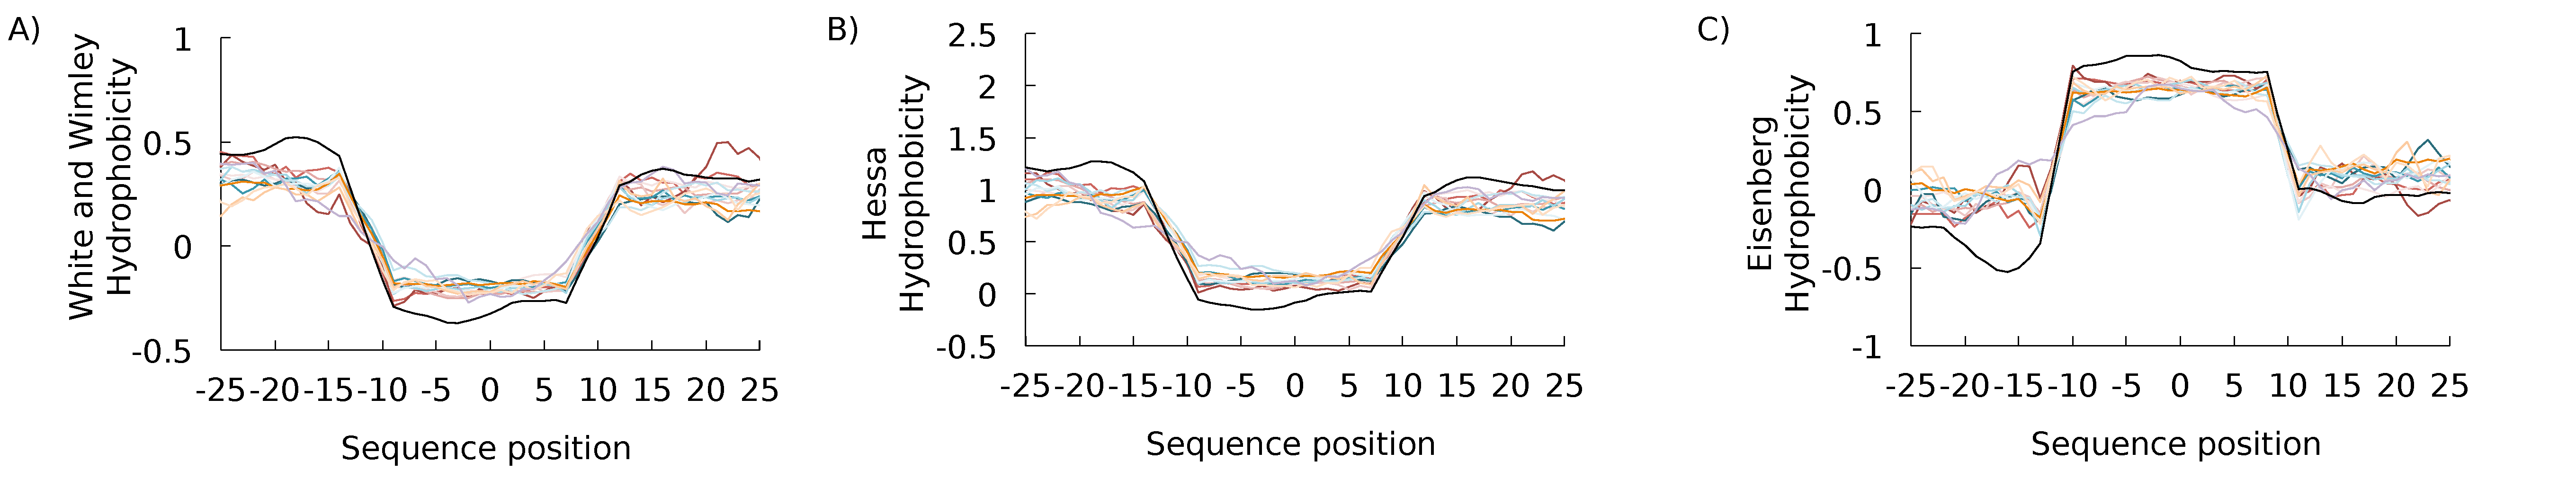
\includegraphics[width=1\textwidth]{NNI_chapter/hydrophobicity_scale_comparison}
\captionof{figure}[There is a difference in the hydrophobic profiles of~\gls{tmh}s from single-pass and multi-pass proteins.]{\textbf{There is a difference in the hydrophobic profiles of~\gls{tmh}s from single-pass and multi-pass proteins.}
The difference in hydrophobicity between the single-pass and multi-pass datasets stratified by number of~\gls{tmh}s is not due to the choice of scale.
As with Figure~\ref{fig:hydrophobicity_single_multi}, UniHuman was stratified according to the number of~\gls{tmh}s in each protein.
The mean amino acid hydrophobicity values of~\gls{tmh}s with a sliding unweighted window of 3 residues from UniHuman proteins at each position were plotted.
To validate the findings presented in Figure \ref{fig:hydrophobicity_single_multi}A, several scales of hydrophobicity were used.
(A) The White and Wimley whole residue scale~\cite{White1999} is based on the partitioning of peptides between water and octanol as well as water to~\gls{popc}.
A positive score indicates a more polar score.
(B) The Hessa biological scale~\cite{Hessa2005}.
The hydrophobicity values represent the free energy exchange during recognition of designed peptide~\gls{tmh}s by the endoplasmic reticulum Sec61 translocon and, therefore, negative values indicate an energetic preference for the interior of a lipid bilayer.
(C) The Eisenberg consensus scale~\cite{Eisenberg1984} is a scale based on the earlier scales from Nozaki and Tanford~\cite{Nozaki1971}, Wolfenden \textit{et al.}~\cite{Wolfenden1981}, Chothia~\cite{Chothia1976}, Janin~\cite{Janin1979} and the von Heijne and Blomberg scale~\cite{VonHeijne1979}.
The scales are normalised according to serine.
A positive score indicates a generally more hydrophobic score.}

\label{fig:hydrophobicity_scale_comparison}
\end{figure}

Leucine is the most abundant residue in~\gls{tmh}s (Figure~\ref{fig:amino_acid_distribution}) and is considered one of the most hydrophobic residues by all hydrophobicity scales.
Therefore, it plays a very influential role in~\gls{tmh} helix-helix and lipid-helix interactions in the membrane and recognition by the insertion machinery.
When looking at the difference in the abundance of leucine between the inner and outer halves, we find that~\gls{tmh}s from single-pass proteins have a trend to contain more leucine residues at the cytoplasmic side of~\gls{tmh}s, particularly in the case of~\gls{tmh}s from single-pass proteins (see Figures~\ref{fig:single_pass_charge_distribution} and~\ref{fig:comp_heatmaps}).

This trend is statistically significant for~\gls{tmh}s in many biological membranes (Table~\ref{table:leucineskewstats}, Figure~\ref{fig:dataset_distributions}).
In the most extreme case of UniCress (single-pass), we see 49\% more leucine residues on the inside leaflet than the outside leaflet (P-value=5.41e-24).
This contrasts with UniCress (multi-pass), in which the skew is far weaker, albeit yet statistically significant.
There are 6\% more leucine residues at the inside half (P-value=2.08e-4).
The trend of having more leucine residues at the cytoplasmic half of the~\gls{tmh} is observed for all datasets (both single- and multi-pass) except for UniArch (single-pass).
The phenomenon is statistically significant with P-value$<$1.e-3 for ExpAll, UniHuman, UniPM and UniCress (both single- and multi-pass).
As with negative charge distribution, UniArch presents a reversed effect compared to other single-pass protein datasets with a 57\% reduction in leucine on the inside leaflet compared to the outside leaflet (P-value=7.25e-6).
However, leucine of~\gls{tmh}s from UniArch multi-pass proteins have no discernible preference for the inside leaflets (4\% more on the inside leaflet, P-value=0.625).

% Table generated by Excel2LaTeX from sheet 'Sheet1'
\begin{table}[htbp]

  \centering
  \captionof{table}[Leucines at the inner and outer leaflets of the membrane in TMHs]{\textbf{Leucines at the inner and outer leaflets of the membrane in TMHs}
  The statistical results when comparing the number of leucine residues from the inner and outer leaflets in each protein in the dataset.
  The number of helices per dataset can be found in Table~\ref{table:acidicresiduesarerare}.
  The Kruskal-Wallis test scores (H statistics) were calculated for leucine residues by comparing the number of leucine residues that were in the inner half of the leaflet with those in the outer half of the leaflet of the database-defined TMH}

    \resizebox{\textwidth}{!}{
    \begin{tabular}{ p{5em} l l r r r l l r r r }
    \toprule
    \multirow{2}[4]{*}{\textbf{Dataset}} & \multicolumn{5}{p{25em} }{\textbf{Single-pass}} & \multicolumn{5}{p{25em} }{\textbf{Multi-pass}} \\
 \cmidrule{2-11}    \multicolumn{1}{ l }{} & \multicolumn{1}{p{5em} }{\textbf{Inside}} & \multicolumn{1}{p{5em} }{\textbf{Outside}} & \multicolumn{1}{p{5em} }{\textbf{Percentage}} & \multicolumn{1}{p{5em} }{\textbf{H statistic}} & \multicolumn{1}{p{5em} }{\textbf{P value}} & \multicolumn{1}{p{5em} }{\textbf{Inside}} & \multicolumn{1}{p{5em} }{\textbf{Outside}} & \multicolumn{1}{p{5em} }{\textbf{Percentage}} & \multicolumn{1}{p{5em} }{\textbf{H statistic}} & \multicolumn{1}{p{5em} }{\textbf{P value}} \\
    \midrule
    ExpAll & 4020  & 3403  & 118.13 & 40.07 & 2.44E-10 & 27,986 & 27,008 & 103.62 & 14.13 & 1.70E-04 \\
    \midrule
    UniHuman & 4982  & 3697  & 134.76 & 193.02 & 6.99E-44 & 25,199 & 22,365 & 112.67 & 195.24 & 2.29E-44 \\
    \midrule
    UniER & 359   & 297   & 120.88 & 8.41  & 3.72E-03 & 1863  & 1764  & 105.61 & 3.98  & 4.61E-02 \\
    \midrule
    UniGolgi & 604   & 513   & 117.74 & 10.74 & 1.05E-03 & 753   & 677   & 111.23 & 5.61  & 1.79E-02 \\
    \midrule
    UniPM & 1485  & 1006  & 147.61 & 98.9  & 2.65E-23 & 6221  & 5577  & 111.55 & 35.21 & 3.00E-09 \\
    \midrule
    UniCress & 1495  & 1005  & 148.76 & 102.05 & 5.41E-24 & 6491  & 6099  & 106.43 & 13.76 & 2.08E-04 \\
    \midrule
    UniFungi & 1389  & 1308  & 106.19 & 3.41  & 6.48E-02 & 14,505 & 14,099 & 102.88 & 6.74  & 9.41E-03 \\
    \midrule
    UniBacilli & 260   & 251   & 103.59 & 0.03  & 8.72E-01 & 1488  & 1335  & 111.46 & 7.59  & 5.89E-03 \\
    \midrule
    UniEcoli & 130   & 100   & 130   & 2.78  & 9.53E-02 & 7251  & 6975  & 103.96 & 5.92  & 1.50E-02 \\
    \midrule
    UniArch & 51    & 118   & 43.22 & 20.13 & 7.25E-06 & 636   & 612   & 103.92 & 0.24  & 6.25E-01 \\
    \bottomrule
    \end{tabular}
    }%
   \label{table:leucineskewstats}

\end{table}%

\begin{figure}[!ht]
\centering
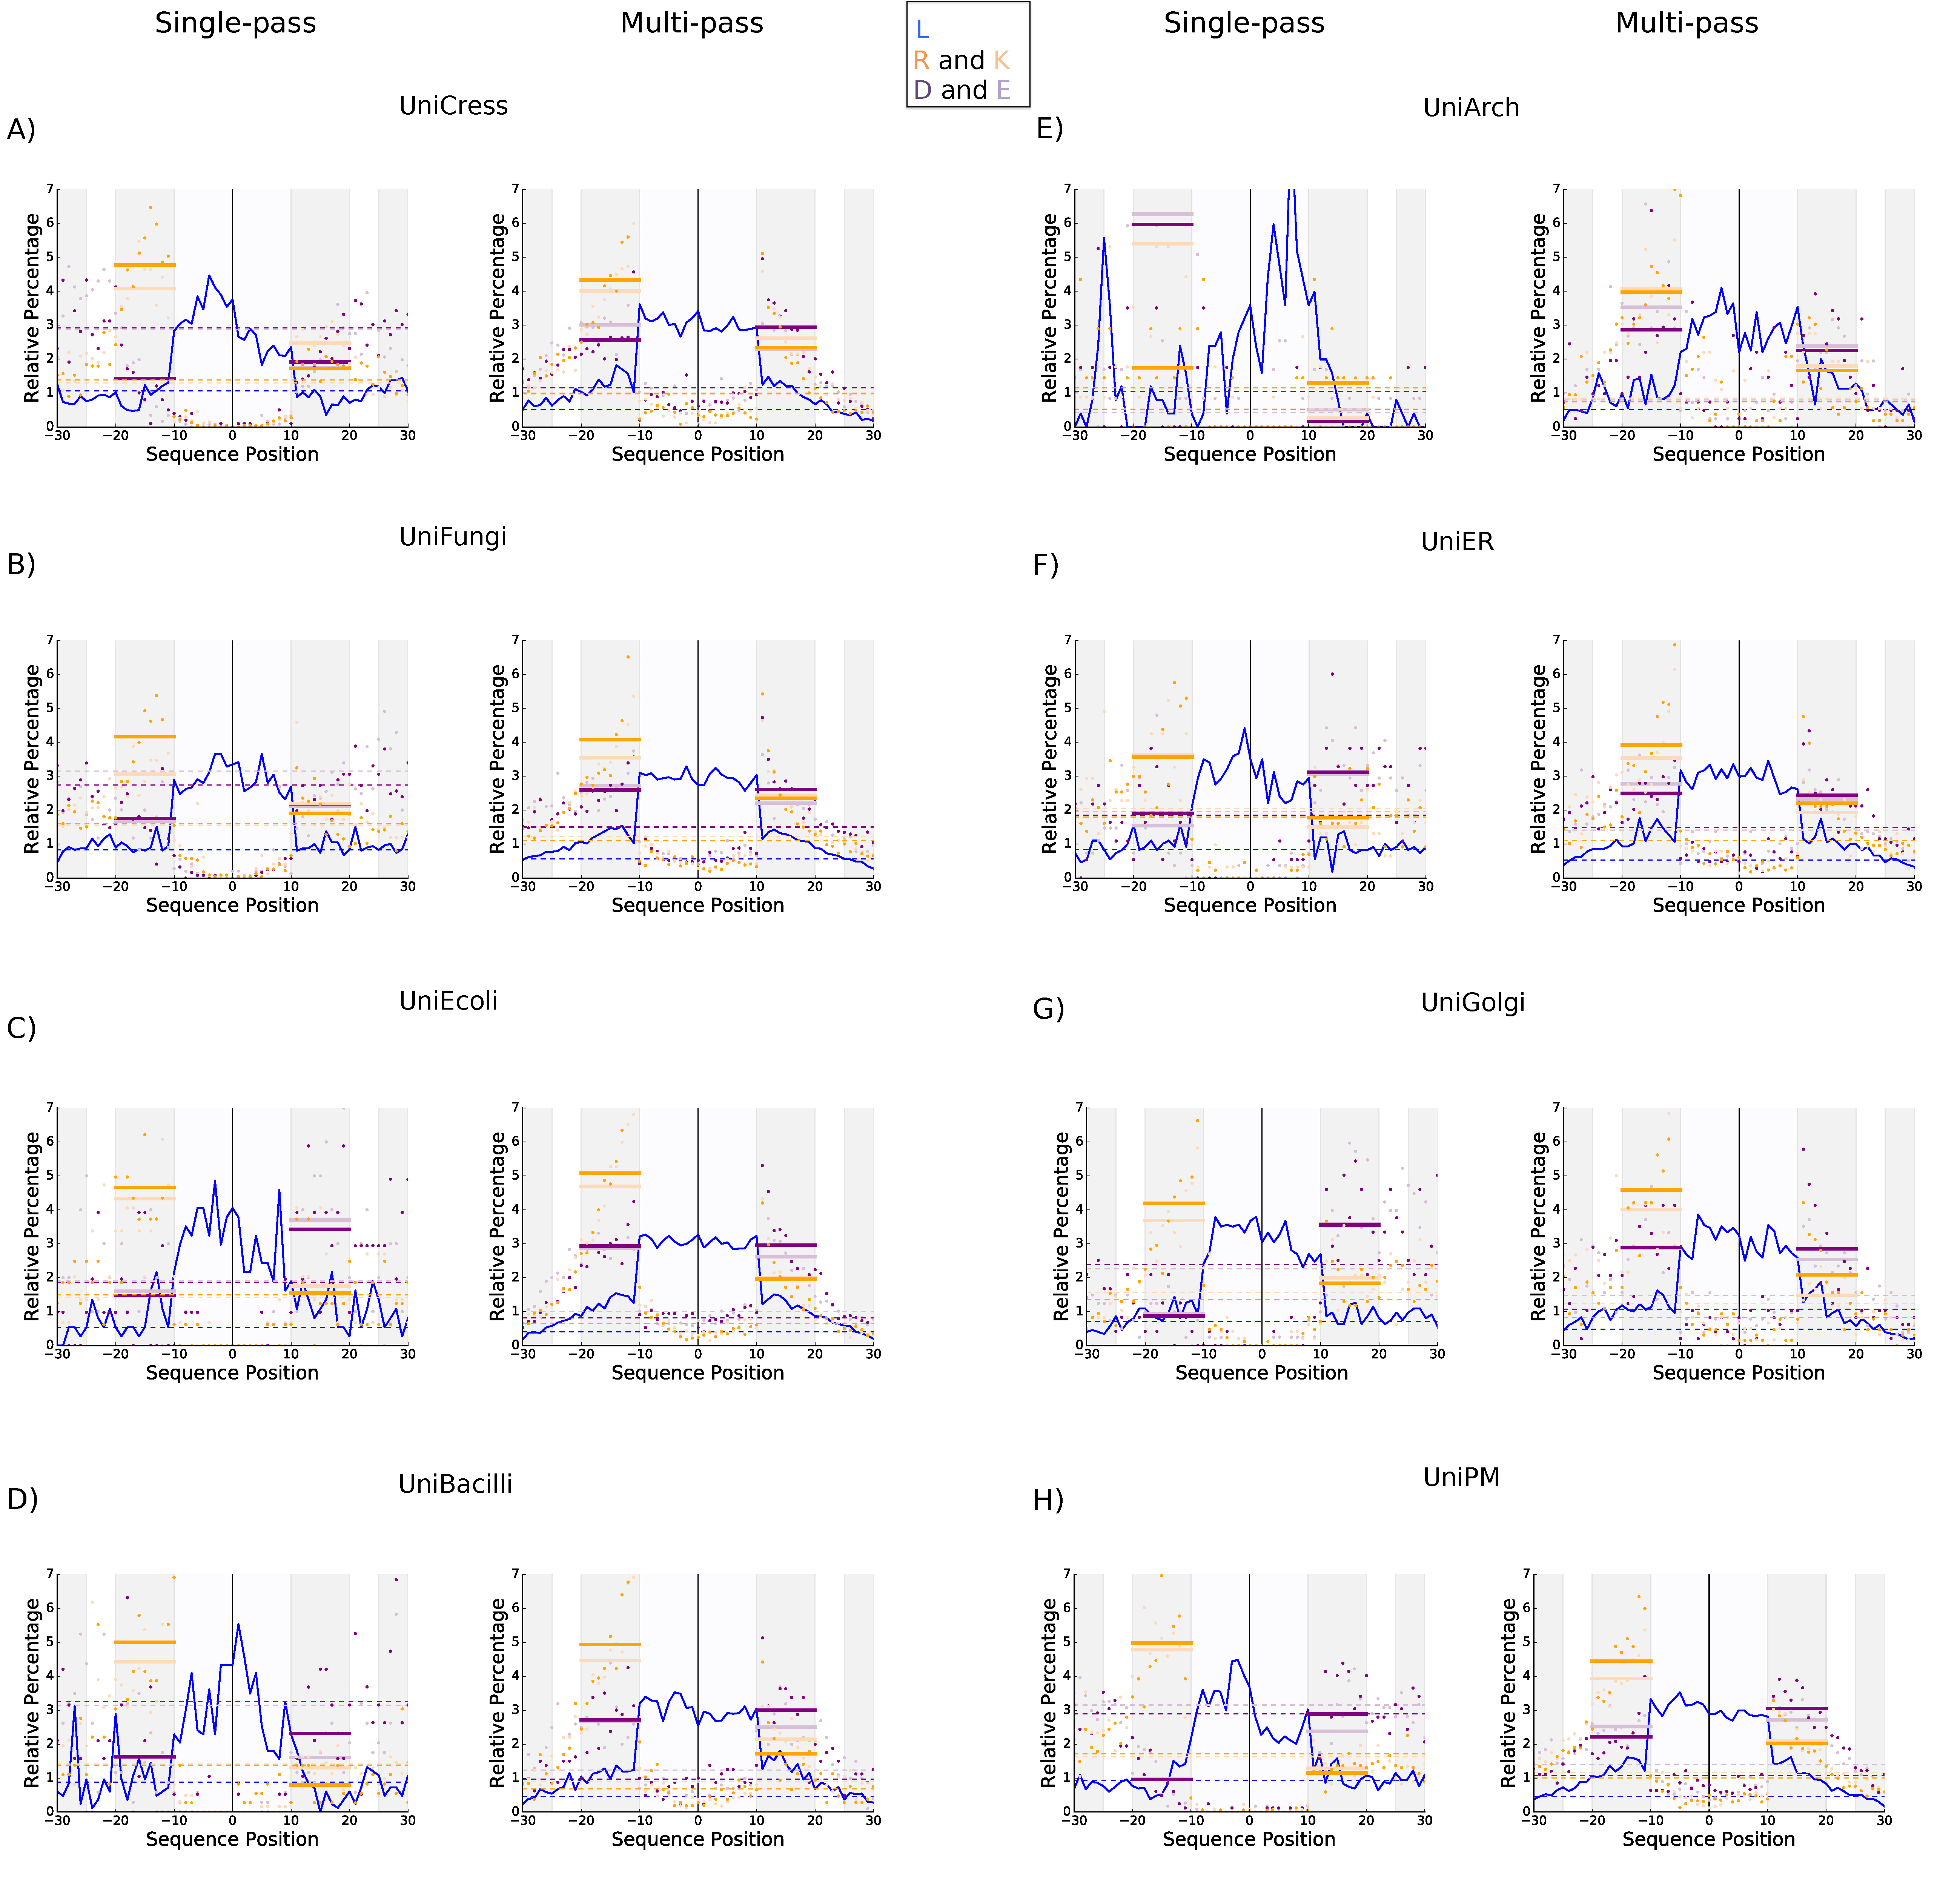
\includegraphics[width=1\textwidth]{NNI_chapter/dataset_distributions}
\captionof{figure}[Comparing charged amino acid distributions in~\gls{tmh}s of multi-pass and single-pass proteins across different species and organelles.]{\textbf{Comparing charged amino acid distributions in~\gls{tmh}s of multi-pass and single-pass proteins across different species and organelles.} The relative percentage distribution of charged residues and leucine was calculated at each position in the~\gls{tmh} with flank lengths of $\pm$20 in different datasets.
The distributions are normalised according to relative percentage distribution.
Aspartic acid and glutamic acid are shown in dark purple and light purple respectively.
Leucine, the most abundant non-polar residue in~\gls{tmh}s, is in blue.
Arginine and lysine are shown in orange.
TMHs from single-pass proteins are on the left and~\gls{tmh}s from multi-pass proteins are on the right for different taxonomic datasets: a UniCress, b UniFungi, c UniEcoli, d UniBacilli, e UniArch, and different organelles: f UniER, g UniGolgi, h UniPM.
As a trend, the negative-outside skew is more present in~\gls{tmh}s from single-pass proteins than multi-pass proteins (Tables 2 and 3).
Another key observation is that in single-pass~\gls{tmh}s there is a propensity for leucine on the inner over the outer leaflet (Table \ref{table:leucineskewstats})}


\label{fig:dataset_distributions}
\end{figure}

\subsection{A negative-outside (or negative-non-inside) signal is present across many membrane types}

We explored the presence of amino acid residue compositional skews described above for human~\gls{tmp}s for those in other taxa and also specifically for human proteins with regard to membranes at various subcellular localisations.
Acidic residues for~\gls{tmh}s from single-pass and multi-pass helices were plotted according to their relative percentage distributions (of the total amount of this residue type in the respective segment) for five taxon-specific datasets UniCress (Figure~\ref{fig:dataset_distributions}A), UniFungi (Figure~\ref{fig:dataset_distributions}B), UniEcoli (Figure~\ref{fig:dataset_distributions}C), UniBacilli (Figure~\ref{fig:dataset_distributions}D), UniArch (Figure~\ref{fig:dataset_distributions}E) and for three organelle-specific datasets UniER (Figure~\ref{fig:dataset_distributions}F), UniGolgi (Figure~\ref{fig:dataset_distributions}G), UniPM (Figure~\ref{fig:dataset_distributions}H).

For single-pass proteins in all taxon-specific datasets (with the exception of UniArch), there are more negative residues at the outside than at the inside.
The skew is statistically significant (see Table~\ref{table:negativeskewsinglepass}, P$<$0.001) except for UniBacilli.
Despite statistical significance found for UniFungi (P-value=1.12e-7 for database-defined and P-value=6.79e-10 for flanks after central alignment; Table~\ref{table:negativeskewsinglepass}), however, the trend is not very strong in this case (Figure~\ref{fig:dataset_distributions}B).
Whereas the skew is just a suppression of negatively charged residues at the inside flank for ExpAll and UniHuman (as well as in UniCress), the bias observed for UniEcoli involves also a negative charge enrichment at the outside flank.
In the case of UniArch (Figure~\ref{fig:dataset_distributions}E), we see a negative inside preference that is 6.0\% in the case of aspartic acid, and 6.3\% for glutamic acid (not shown), with much lower values close to 0\% on the outside.
Whilst the difference is statistically significant for both~\gls{tmh}s (Table~\ref{table:negativeskewsinglepass}) from single-pass proteins (P-value=1.83e-12 and P-value=1.43e-11 for two versions of flank determination) and multi-pass proteins (P-values 4.72e-3, 7.81e-3, 1.28e-4 for three versions of flank determination, see Tables 3A and 3B), the distribution along the position axis is heavily fluctuating, maybe as a result of the small size of the dataset.
However, one can assuredly assign a ``negative-inside'' tendency to the flanking regions of Archaean~\gls{tmh}s.

In the human organelle datasets, we see trend shifts at different stages in the secretory pathway.
In UniER, there is an enrichment of negative charge on the outside flank of 1--1.5\% that is comparable to the magnitude of the positive inside signal.
In UniGolgi, there is a suppression of negatively charged residues on the inside flank as well as an enrichment on the inside flank resulting in \(\sim\)2\% distribution difference.
For UniPM, there is a negative-inside suppression (but no outside enrichment) as well as a positive-inside signal.
All observed trends are statistically significant (see Table~\ref{table:negativeskewsinglepass}, P$<$1.e-5).

For multi-pass~\gls{tmh} proteins, we see either the same trends but in a weaker form or no skews are observed at all as inspection of the graphs in Figure~\ref{fig:dataset_distributions} shows.
For datasets UniER, UniGolgi, UniCress, UniFungi, and UniBacilli, the hypothesis of equal distribution of negatively charged residues cannot be rejected (P-value$>$0.001, see Table 3); thus, a skew is statistically non-significant.
Although UniPM has a statistically significant bias (P-value$<$4.30e-12, Table 3), the trends are more subtle and most present for aspartic acid of UniPM\@.
We see many more negative and positive charges tolerated within the multi-pass~\gls{tmh}s themselves throughout all datasets (Table \ref{table:acidicresiduesarerare}).
To note, there is a positive-inside rule for all multi-pass datasets studied herein.

To conclude, we find that negative-charge bias distribution is a feature of single-pass protein~\gls{tmh}s that is present across many membrane types and it can have the form of a negative charge suppression at the inside flank or an enrichment of those charges at the outside flank.

\subsection{Amino acid compositional skews in relation to~\gls{tmh} complexity and anchorage function}

\begin{figure}[p]
\centering
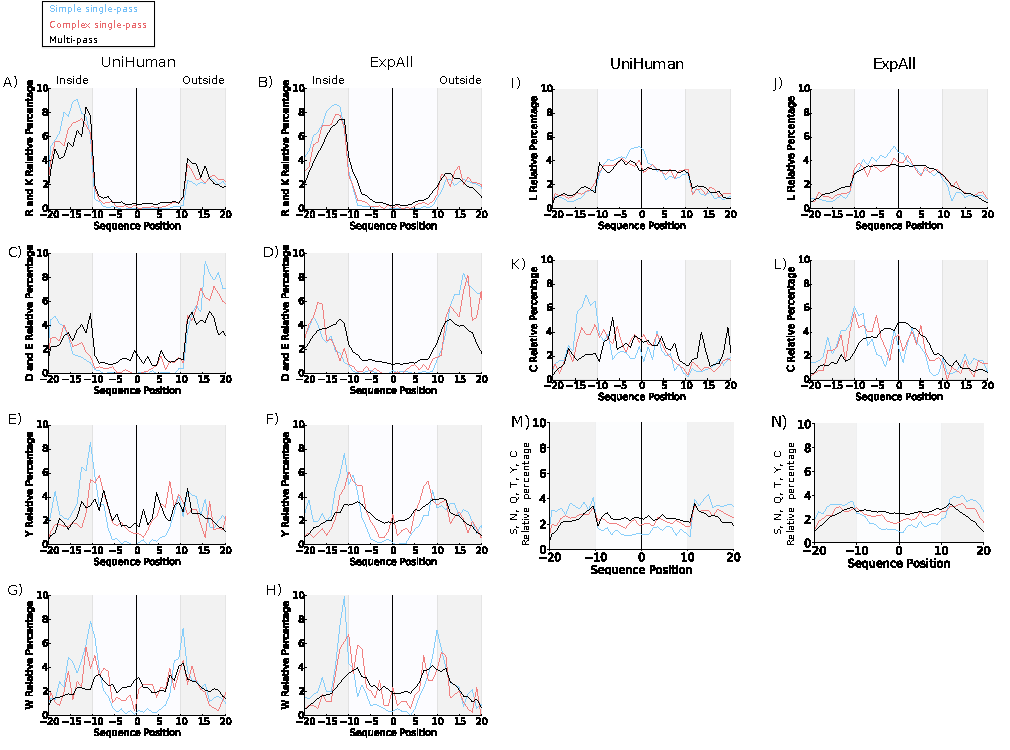
\includegraphics[height=0.7\textheight]{NNI_chapter/complexity_datasets}
\captionof{figure}[Comparing the amino acid relative percentage distributions of simple and complex~\gls{tmh}s from single-pass proteins and~\gls{tmh}s from multi-pass proteins.]{\textbf{Comparing the amino acid relative percentage distributions of simple and complex~\gls{tmh}s from single-pass proteins and~\gls{tmh}s from multi-pass proteins.} Comparing the amino acid relative percentage distributions of simple and complex~\gls{tmh}s from single-pass proteins and~\gls{tmh}s from multi-pass proteins.
TMSOC was used to calculate which single-pass~\gls{tmh}s were complex and which were simple from ExpAll and UniHuman datasets.
Simple~\gls{tmh}s are typically anchors without necessarily having other functions (Wong \textit{et al.}~\cite{Wong2010}).
The relative percentages from single-pass simple (shown in light blue), single-pass complex (red), and multi-pass protein~\gls{tmh}s (black) were plotted for (a, c, e, g, i and k) UniHuman and (b, d, f, h, j and l) ExpAll for (a and b) positive residues, (c and d) negative residues, (e and f) tyrosine, (g and h) tryptophan, (i and j) leucine and (k and l) cysteine.
The slopes are statistically compared in Tables 5 and 6, and as a trend, the profiles of complex~\gls{tmh}s are more similar to multi-pass~\gls{tmh} profiles than simple~\gls{tmh}s are to multi-pass~\gls{tmh}s}

\label{fig:complexity_datasets}
\end{figure}

In previous work, we studied the relationship of~\gls{tmh} composition, sequence complexity and function~\cite{Wong2010, Wong2011, Wong2012} and concluded that simple~\gls{tmh}s are more probably responsible for simple membrane anchorage, whereas complex~\gls{tmh}s have a biological function beyond just anchorage.
We wished to see how the skews observed in this work relate to that classification.
Therefore, the single-pass~\gls{tmh}s from UniHuman and ExpAll were separated into subsets of simple, twilight, and complex~\gls{tmh}s using TMSOC~\cite{Wong2011, Wong2012}.
The relative percentages of eight residue types (L, D, E, R, K, Y, W, C\@; normalisation with the total amount of residues of that amino acid type in all sequence segments considered) were plotted along the sequence position for simple and complex helices (Figure~\ref{fig:complexity_datasets}).
Of UniHuman single-pass proteins, there were 889 records with simple~\gls{tmh}s and 570 with complex~\gls{tmh}s (Figure~\ref{fig:complexity_datasets}B).
In ExpAll, 769~\gls{tmh}s from single-pass proteins were simple~\gls{tmh}s and 570 were complex~\gls{tmh}s.

It is visually apparent (Figure~\ref{fig:complexity_datasets}) that there are (i) stronger skews and more inside-outside disparities in simple single-pass~\gls{tm}s than in complex single-pass~\gls{tm}s and (ii) greater similarities between single-pass complex TM regions and those from multi-pass proteins compared with simple single-pass~\gls{tm}s in comparison with either of the other two distributions.
To examine the statistical significance of these observations, we compared the amino acid distributions (K, R, K+R, D, E, D+E, Y, W, L, C) across the range of~\gls{tmh}s with flank lengths $\pm$10 residues using the~\gls{ks},~\gls{kw} and the \({\chi}^{2}\) statistical tests.
To note, the~\gls{ks} test scrutinises for significant maximal absolute differences between distribution curves; the gls{kw} test is after skews between distributions and the \({\chi}^{2}\) statistical test checks the average difference between distributions.
Calculations were carried out over single-pass complex, single-pass simple and multi-pass~\gls{tmh} datasets from both ExpAll and UniHuman (for P-values and Bahadur slopes, Table~\ref{table:unihumanbahadur} (dataset UniHuman) and Table~\ref{table:expallbahadur} (dataset ExpAll)).

\begin{table}[htbp]

  \centering
  \captionof{table}[Simple TMHs are less similar than complex TMHs to TMHs from multi-pass proteins in UniHuman]{\textbf{Simple TMHs are less similar than complex TMHs to TMHs from multi-pass proteins in UniHuman}
  The statistical results were gathered by comparing complex single-pass TMHs, simple TMHs from single-pass proteins and TMHs from multi-pass proteins in UniHuman.
  The abundance of different residues at each position when using the centrally aligned TMH approach was compared with several statistical tests (the~\gls{ks},~\gls{kw} and the $\chi^2$ statistical tests) and the Bahadur slope values of those results}
    \resizebox{\textwidth}{!}{
    \tiny
    \begin{tabular}{ p{5em} l l l l l l }
    \toprule
    \multirow{2}[4]{*}{Residues} & \multicolumn{3}{p{15em} }{P values for $\chi^2$} & \multicolumn{3}{p{15em} }{Bahadur slopes for $\chi^2$} \\
\cmidrule{2-7}    \multicolumn{1}{ l }{} & \multicolumn{1}{p{5em} }{Simple-vs-complex} & \multicolumn{1}{p{5em} }{Simple-vs-multi} & \multicolumn{1}{p{5em} }{Complex-vs-multi} & \multicolumn{1}{p{5em} }{Simple-vs-complex} & \multicolumn{1}{p{5em} }{Simple-vs-multi} & \multicolumn{1}{p{5em} }{Complex-vs-multi} \\
    \midrule
    R    & 3.20E-06 & 7.38E-02 & 1.24E-01 & 6.61E-03 & 2.20E-03 & 1.27E-04 \\
    \midrule
    K    & 2.23E-03 & 4.99E-02 & 2.14E-01 & 3.99E-03 & 3.70E-03 & 1.18E-04 \\
    \midrule
    D    & 1.67E-09 & 3.06E-01 & 3.02E-01 & 3.34E-02 & 3.24E-03 & 1.20E-04 \\
    \midrule
    E    & 3.80E-07 & 2.34E-01 & 2.31E-01 & 1.81E-02 & 3.05E-03 & 1.36E-04 \\
    \midrule
    Y    & 3.86E-01 & 3.97E-01 & 2.11E-01 & 1.06E-03 & 1.47E-03 & 8.25E-05 \\
    \midrule
    W    & 3.77E-03 & 2.97E-01 & 3.84E-01 & 8.52E-03 & 2.73E-03 & 1.13E-04 \\
    \midrule
    L    & 3.59E-01 & 2.88E-01 & 3.21E-01 & 1.52E-04 & 3.92E-04 & 1.69E-05 \\
    \midrule
    C    & 6.44E-01 & 3.97E-01 & 3.41E-01 & 4.29E-04 & 1.29E-03 & 8.57E-05 \\
    \midrule
    R+K & 2.19E-02 & 2.83E-01 & 2.52E-01 & 1.11E-03 & 6.33E-04 & 4.68E-05 \\
    \midrule
    D+E & 1.47E-03 & 2.86E-01 & 2.79E-01 & 4.59E-03 & 1.49E-03 & 6.15E-05 \\
    \midrule
    \multicolumn{1}{ l }{} & \multicolumn{3}{p{15em} }{P values for Kolmogorov-Smirnov} & \multicolumn{3}{p{15em} }{Bahadur slopes for Kolmogorov-Smirnov} \\
    \midrule
    \multicolumn{1}{ l }{} & \multicolumn{1}{p{5em} }{Simple-vs-complex} & \multicolumn{1}{p{5em} }{Simple-vs-multi} & \multicolumn{1}{p{5em} }{Complex-vs-multi} & \multicolumn{1}{p{5em} }{Simple-vs-complex} & \multicolumn{1}{p{5em} }{Simple-vs-multi} & \multicolumn{1}{p{5em} }{Complex-vs-multi} \\
    \midrule
    R    & 2.31E-01 & 3.57E-04 & 1.08E-02 & 7.66E-04 & 6.71E-03 & 2.76E-04 \\
    \midrule
    K    & 4.31E-02 & 2.18E-03 & 8.93E-01 & 2.06E-03 & 7.56E-03 & 8.68E-06 \\
    \midrule
    D    & 1.39E-01 & 5.02E-06 & 1.08E-02 & 3.26E-03 & 3.34E-02 & 4.52E-04 \\
    \midrule
    E    & 7.96E-02 & 1.58E-05 & 1.08E-02 & 3.10E-03 & 2.32E-02 & 4.20E-04 \\
    \midrule
    Y    & 7.96E-02 & 2.22E-02 & 2.31E-01 & 2.81E-03 & 6.07E-03 & 7.78E-05 \\
    \midrule
    W    & 2.31E-01 & 9.06E-04 & 4.31E-02 & 2.24E-03 & 1.58E-02 & 3.70E-04 \\
    \midrule
    L    & 2.31E-01 & 2.31E-01 & 5.31E-01 & 2.17E-04 & 4.61E-04 & 9.42E-06 \\
    \midrule
    C    & 1.39E-01 & 3.61E-01 & 3.61E-01 & 1.93E-03 & 1.42E-03 & 8.10E-05 \\
    \midrule
    R+K & 7.96E-02 & 1.33E-04 & 7.96E-02 & 7.35E-04 & 4.48E-03 & 8.60E-05 \\
    \midrule
    D+E & 4.31E-02 & 1.58E-05 & 4.98E-03 & 2.21E-03 & 1.31E-02 & 2.55E-04 \\
    \midrule
    \multicolumn{1}{ l }{} & \multicolumn{3}{p{15em} }{P values for Kruskal-Wallis} & \multicolumn{3}{p{15em} }{Bahadur slopes for Kruskal-Wallis} \\
    \midrule
    \multicolumn{1}{ l }{} & \multicolumn{1}{p{5em} }{Simple-vs-complex} & \multicolumn{1}{p{5em} }{Simple-vs-multi} & \multicolumn{1}{p{5em} }{Complex-vs-multi} & \multicolumn{1}{p{5em} }{Simple-vs-complex} & \multicolumn{1}{p{5em} }{Simple-vs-multi} & \multicolumn{1}{p{5em} }{Complex-vs-multi} \\
    \midrule
    R    & 2.19E-01 & 5.06E-02 & 2.37E-01 & 7.92E-04 & 2.52E-03 & 8.79E-05 \\
    \midrule
    K    & 2.90E-01 & 1.33E-01 & 7.00E-01 & 8.11E-04 & 2.49E-03 & 2.73E-05 \\
    \midrule
    D    & 3.50E-01 & 1.81E-02 & 2.81E-01 & 1.74E-03 & 1.10E-02 & 1.27E-04 \\
    \midrule
    E    & 2.59E-01 & 5.65E-02 & 1.78E-01 & 1.65E-03 & 6.04E-03 & 1.60E-04 \\
    \midrule
    Y    & 6.03E-01 & 4.53E-01 & 4.41E-01 & 5.62E-04 & 1.26E-03 & 4.34E-05 \\
    \midrule
    W    & 4.19E-01 & 1.84E-01 & 5.70E-01 & 1.33E-03 & 3.81E-03 & 6.62E-05 \\
    \midrule
    L    & 6.37E-01 & 4.88E-01 & 9.77E-01 & 6.68E-05 & 2.25E-04 & 3.47E-07 \\
    \midrule
    C    & 5.00E-01 & 2.22E-01 & 9.62E-01 & 6.76E-04 & 2.10E-03 & 3.11E-06 \\
    \midrule
    R+K & 1.87E-01 & 8.67E-02 & 4.08E-01 & 4.86E-04 & 1.23E-03 & 3.05E-05 \\
    \midrule
    D+E & 1.68E-01 & 4.52E-02 & 1.91E-01 & 1.25E-03 & 3.68E-03 & 7.97E-05 \\
    \bottomrule
    \end{tabular}%
    }%
   \label{table:unihumanbahadur}

\end{table}%

\begin{table}[htbp]

  \centering
  \captionof{table}[Simple TMHs are less similar than complex TMHs to TMHs from multi-pass proteins in ExpAll]{\textbf{Simple TMHs are less similar than complex TMHs to TMHs from multi-pass proteins in ExpAll}
  As in Table~\ref{table:unihumanbahadur}, the statistical results were gathered by comparing complex single-pass TMHs, simple TMHs from single-pass proteins and TMHs from multi-pass proteins; however, in this case only ExpAll is used.
  The abundance of different residues at each position when using the centrally aligned TMH approach was compared with several statistical tests (the~\gls{ks},~\gls{kw} and the $\chi^2$ statistical tests) and the Bahadur slope values of those results}
    \resizebox{\textwidth}{!}{
    \tiny
    \begin{tabular}{ p{5em} l l l l l l }
    \toprule
    \multirow{2}[4]{*}{Residues} & \multicolumn{3}{p{15em} }{P values for $\chi^2$} & \multicolumn{3}{p{15em} }{Bahadur slopes for  $\chi^2$} \\
\cmidrule{2-7}    \multicolumn{1}{ l }{} & \multicolumn{1}{p{5em} }{Simple-vs-complex} & \multicolumn{1}{p{5em} }{Simple-vs-multi} & \multicolumn{1}{p{5em} }{Complex-vs-multi} & \multicolumn{1}{p{5em} }{Simple-vs-complex} & \multicolumn{1}{p{5em} }{Simple-vs-multi} & \multicolumn{1}{p{5em} }{Complex-vs-multi} \\
    \midrule
     R    & 5.10E-06 & 2.98E-01 & 5.10E-06 & 9.17E-03 & 1.61E-03 & 6.23E-05 \\
    \midrule
     K    & 2.35E-03 & 1.85E-01 & 2.35E-03 & 4.81E-03 & 3.88E-03 & 9.78E-05 \\
    \midrule
     D    & 2.61E-08 & 1.84E-01 & 2.61E-08 & 4.15E-02 & 7.90E-03 & 1.41E-04 \\
    \midrule
     E    & 2.38E-10 & 2.04E-01 & 2.38E-10 & 3.88E-02 & 7.08E-03 & 1.22E-04 \\
    \midrule
     Y    & 3.03E-01 & 3.11E-01 & 3.03E-01 & 2.01E-03 & 2.49E-03 & 5.51E-05 \\
    \midrule
     W    & 4.21E-03 & 4.29E-01 & 4.21E-03 & 1.11E-02 & 4.76E-03 & 6.46E-05 \\
    \midrule
     L    & 3.79E-01 & 3.04E-01 & 3.79E-01 & 2.28E-04 & 4.66E-04 & 1.50E-05 \\
    \midrule
     C    & 3.87E-01 & 2.52E-01 & 3.87E-01 & 1.75E-03 & 3.28E-03 & 1.48E-04 \\
    \midrule
     R+K & 7.16E-04 & 2.52E-01 & 7.16E-04 & 2.80E-03 & 1.28E-03 & 3.76E-05 \\
    \midrule
     D+E & 3.58E-05 & 2.94E-01 & 3.58E-05 & 1.03E-02 & 1.94E-03 & 4.90E-05 \\
    \midrule
    \multicolumn{1}{ l }{} & \multicolumn{3}{p{15em} }{P values for Kolmogorov-Smirnov} & \multicolumn{3}{p{15em} }{Bahadur slopes for Kolmogorov-Smirnov} \\
    \midrule
    \multicolumn{1}{ l }{} & \multicolumn{1}{p{5em} }{Simple-vs-complex} & \multicolumn{1}{p{5em} }{Simple-vs-multi} & \multicolumn{1}{p{5em} }{Complex-vs-multi} & \multicolumn{1}{p{5em} }{Simple-vs-complex} & \multicolumn{1}{p{5em} }{Simple-vs-multi} & \multicolumn{1}{p{5em} }{Complex-vs-multi} \\
    \midrule
     R    & 3.61E-01 & 4.31E-02 & 3.61E-01 & 7.66E-04 & 7.79E-03 & 1.62E-04 \\
    \midrule
     K    & 4.31E-02 & 8.93E-01 & 4.31E-02 & 2.49E-03 & 1.05E-02 & 6.57E-06 \\
    \midrule
     D    & 1.39E-01 & 2.18E-03 & 1.39E-01 & 4.68E-03 & 3.61E-02 & 5.10E-04 \\
    \midrule
     E    & 5.31E-01 & 1.33E-04 & 5.31E-01 & 1.11E-03 & 2.81E-02 & 6.87E-04 \\
    \midrule
     Y    & 2.31E-01 & 9.06E-04 & 2.31E-01 & 2.47E-03 & 6.26E-03 & 3.30E-04 \\
    \midrule
     W    & 5.31E-01 & 4.98E-03 & 5.31E-01 & 1.29E-03 & 1.13E-02 & 4.04E-04 \\
    \midrule
     L    & 2.31E-01 & 2.31E-01 & 2.31E-01 & 3.45E-04 & 2.12E-03 & 1.85E-05 \\
    \midrule
     C    & 5.31E-01 & 3.61E-01 & 5.31E-01 & 1.16E-03 & 8.91E-04 & 1.09E-04 \\
    \midrule
     R+K & 1.39E-01 & 2.31E-01 & 1.39E-01 & 7.61E-04 & 4.82E-03 & 4.00E-05 \\
    \midrule
     D+E & 1.39E-01 & 9.06E-04 & 1.39E-01 & 1.99E-03 & 1.41E-02 & 2.80E-04 \\
    \midrule
    \multicolumn{1}{ l }{} & \multicolumn{3}{p{15em} }{P values for Kruskal-Wallis} & \multicolumn{3}{p{15em} }{Bahadur slopes for Kruskal-Wallis} \\
    \midrule
    \multicolumn{1}{ l }{} & \multicolumn{1}{p{5em} }{Simple-vs-complex} & \multicolumn{1}{p{5em} }{Simple-vs-multi} & \multicolumn{1}{p{5em} }{Complex-vs-multi} & \multicolumn{1}{p{5em} }{Simple-vs-complex} & \multicolumn{1}{p{5em} }{Simple-vs-multi} & \multicolumn{1}{p{5em} }{Complex-vs-multi} \\
    \midrule
     R    & 4.37E-01 & 3.92E-01 & 4.37E-01 & 6.24E-04 & 2.52E-03 & 4.82E-05 \\
    \midrule
     K    & 3.83E-01 & 6.93E-01 & 3.83E-01 & 7.62E-04 & 2.88E-03 & 2.13E-05 \\
    \midrule
     D    & 4.49E-01 & 1.81E-01 & 4.49E-01 & 1.90E-03 & 1.06E-02 & 1.42E-04 \\
    \midrule
     E    & 7.64E-01 & 1.94E-01 & 7.64E-01 & 4.71E-04 & 9.05E-03 & 1.26E-04 \\
    \midrule
     Y    & 8.32E-01 & 3.36E-01 & 8.32E-01 & 3.09E-04 & 9.63E-04 & 5.15E-05 \\
    \midrule
     W    & 7.25E-01 & 1.36E-01 & 7.25E-01 & 6.53E-04 & 5.44E-03 & 1.52E-04 \\
    \midrule
     L    & 7.15E-01 & 7.95E-01 & 7.15E-01 & 7.90E-05 & 3.41E-04 & 2.90E-06 \\
    \midrule
     C    & 8.47E-01 & 9.54E-01 & 8.47E-01 & 3.05E-04 & 4.26E-05 & 5.06E-06 \\
    \midrule
     R + K & 2.89E-01 & 5.13E-01 & 2.89E-01 & 4.79E-04 & 1.41E-03 & 1.82E-05 \\
    \midrule
     D+E & 4.94E-01 & 2.07E-01 & 4.94E-01 & 7.11E-04 & 4.14E-03 & 6.29E-05 \\
    \bottomrule
    \end{tabular}%
    }%
   \label{table:expallbahadur}

\end{table}%

Many low P-values in Tables~\ref{table:unihumanbahadur} and~\ref{table:expallbahadur} indicate significant differences between the three distributions studied.
For the UniHuman dataset (Table~\ref{table:unihumanbahadur}), we find most striking, significant differences between charged residue distributions (R, K, D, E) of simple and complex single-pass~\gls{tmh}+flank regions (\({\chi}^{2}\) P-value$<$2.23e-3 for single amino acid types).
Similarly, simple single-pass~\gls{tmh}+flank segments differ significantly from multi-pass~\gls{tmh}+flank segments (\gls{kw} test P-values$<$3.e-2 for R, K, D, E, Y, W amino acid types as well as for K+R and D+E).
The trends are the same for the ExpAll dataset (Table~\ref{table:expallbahadur}): simple and complex single-pass~\gls{tmh}+flank regions differ in charged amino acid type distributions (\({\chi}^{2}\) P-value$<$4.21e-3 for all cases), as well as simple single-pass and multi-pass ones, do (\gls{kw} test P-values$<$5.e-2 for R, D, E, Y, W amino acid types and D+E).

Whereas P-value tests for significant differences between distributions depend strongly on the amount of data, the more informative Bahadur slopes that measure the distance from the zero hypothesis are independent of the amount of data~\cite{Bahadur1967, Bahadur1971, Sunyaev1998}.
As we can see in Tables~\ref{table:unihumanbahadur} and~\ref{table:expallbahadur}, the absolute Bahadur slopes for the simple single-pass to multi-pass comparison are always larger (even by at least an order of magnitude): (ii) for all three statistical tests applied (\({\chi}^{2}\),~\gls{ks} and~\gls{kw}), (ii) for all amino acid types, for K+R and E+D and (iii) for both datasets UniHuman and ExpAll.
Thus, complex single-pass~\gls{tmh}+flanks have compositional properties that are indeed very similar to those of multi-pass ones (which are known to have a large fraction of complex~\gls{tmh}s~\cite{Wong2011, Wong2012}).
This strong evidence implies that the actual issue is not so much about single- and multi-pass~\gls{tmh} segments but between simple and complex~\gls{tmh}s where the first are exclusively guided by the anchor requirements whereas the latter have more complex restraints to fulfil.

Several distribution features of simple~\gls{tmh}s from single-pass proteins when compared to complex~\gls{tmh}s from single-pass proteins and~\gls{tmh}s from multi-pass proteins that contribute to the statistical differences (Figure~\ref{fig:complexity_datasets}) are especially notable.
There is a more pronounced trend for positively charged residues and tyrosine to be preferentially located on the inside flanks and for negatively charged residues to be on the outside flanks.
The symmetrical peaks in the percentage distribution of tyrosine in complex single-pass~\gls{tmh}s are more akin to multi-pass~\gls{tmh}s, whereas in simple~\gls{tmh}s the distribution resembles a more typical single-pass helix (compare with Figure~\ref{fig:single_pass_charge_distribution}).
Furthermore, the depression of charged residues within the~\gls{tmh} itself is strongest in simple single-pass~\gls{tmh}s.

To emphasise, tryptophan is essentially not tolerated within the simple~\gls{tmh}s and there are higher peaks of tryptophan occurrence at either flank.
We also see a strong inside skew for leucine clustering within the core of simple~\gls{tmh}s which is not present in the ``flatter'' distributions of complex single-pass~\gls{tmh}s and~\gls{tmh}s from multi-pass proteins.

There is obviously a cysteine-inside preference for simple, single-pass~\gls{tmh}s but less in complex, multi-pass~\gls{tmh}s (Figure~\ref{fig:complexity_datasets}).
This conclusion is contrary to a previous study~\cite{Nakashima1992} but that deduction was drawn from a much smaller dataset of 45 single-pass~\gls{tmh}s and 24 multi-pass~\gls{tmp}s.

\section{Discussion}

The ``negative-outside/non-negative inside'' skew in~\gls{tmh}s and their flanks is statistically significant
We have seen that, consistently throughout the datasets, there is a trend for generally rare negatively charged residues to prefer the outside flank of a~\gls{tmh} rather than the inside (and to almost completely avoid the~\gls{tmh} itself); be it by suppression on the inside and/or enrichment on the outside.
The trend is much stronger in single-pass protein datasets than in multi-pass protein datasets.
However as we elaborated on further, the real crux of the bias appears to be associated with the~\gls{tmh} being simple or complex~\cite{Wong2011, Wong2012}, thus, whether or not the~\gls{tmh} has a role beyond anchorage.
The existence of this bias has implications for topology prediction of proteins with~\gls{tmh}s, engineering membrane proteins as well as for models of protein transport via membranes and protein-membrane stability considerations.

It should be noted that the controversy in the scientific community about the existence of a negative charge bias at~\gls{tmh}s was mainly with regard to multi-pass~\gls{tmp}s.
Despite having access to much larger, better annotated sequence datasets and many more 3D structures than our predecessors, we also had our share of difficulties here (see Results section III and Table 3).
The straightforward approach results in inconclusive statistical tests if datasets become small (for example, if selections are restricted to subcellular localisations, 3D structures or if very harsh sequence redundancy criteria are applied) and, especially, if~\gls{tmh}s with very short or no flanks are included.
Therefore in the case of multi-pass proteins, we studied flanks as taken from the TM boundaries in the databases under several conditions: (i) without allowing flank overlap between neighbouring~\gls{tmh}s, (ii) as subset of (i) but with requiring some minimal flank length at either side, (iii) with overlapping flanks.
We also studied flanks after central alignment of~\gls{tmh}s and assuming standardised~\gls{tmh} length.
Multi-pass~\gls{tmh}s (without overlapping flanks) do not show statistically significant negative charge bias under condition (i) but, apparently, due to many~\gls{tmh}s without any or super-short flanks at least at one side.
Significance appears as soon as subsets of~\gls{tmh}s with flanks at both sides are studied.
Not surprisingly, there is no charge bias if there are no flanks in the first place.
It is perhaps worth noting that the results from multi-pass~\gls{tmh}s with overlapping flanks may involve amplification of skews since it involves multiple counting of the same residues.
Given the redundancy threshold of UniRef90, we cannot rule out that these statistical skews are the result of a trend from only a small sub-group of~\gls{tmp}s which is being amplified.
Hence, we also needed to observe if these same observed biases were true in condition (ii), which is indeed the case.

As the ``negative-outside/negative-not-inside'' skew is widely observed among varying taxa and subcellular localisations with statistical significance, it appears to, at least to a certain extent, be caused by physical reasons and be associated with the background membrane potential.
Several earlier considerations and observation support this thought: (i) Firstly, a concert between the negative and positive charge on the~\gls{tmh} flanks drives anchorage and the direction of insertion of engineered~\gls{tmh}s~\cite{Sipos1993, Hartmann1989}.
(ii) The inner leaflet of the plasmalemma tends to be more negatively charged~\cite{Zachowski1993}.
Specifically, phosphatidylserine was found to distribute in the cytosolic leaflets of the plasma membrane and it was found to electrostatically interact with moderately positive-charged proteins enough to redirect the proteins into the endocytic pathway~\cite{Yeung2008}.
The negative charge of proteins at the inside of the plasma-membrane would decrease the anchoring potency of the~\gls{tmh} via electrostatic repulsion.
(iii) Thirdly in membranes that maintain a membrane potential, there are inevitably electrical forces acting on charged residues during chain translocation as this influences the translocon machinery when orienting the~\gls{tmh}.
Therefore, it is no surprise that we see an inside-outside bias for negatively charged residues that is opposite to the one for positively charged residues.
The negative charges in~\gls{tmh} residues have been shown to experience an electrical pulling force as they pass through the bacterial SecYEG translocon import~\cite{Ismail2012, Ismail2015}.
Also, they are known to be involved in intra-membrane helix-helix interactions~\cite{Meindl-Beinker2006}.
For example, aspartic acid and glutamic acid can drive efficient di- or trimerisation of~\gls{tmh}s in lipid bilayers and, furthermore, that aspartic acid interactions with neighbouring~\gls{tmh}s can directly increase insertion efficiency of marginally hydrophobic~\gls{tmh}s via the Sec61 translocon~\cite{Meindl-Beinker2006}.
In support of this, less acidic residues are found in single-pass~\gls{tmh}s, among which only some will undergo intra-membrane helix-helix interactions.
As the mutation studies have shown negative charge as a topological determinant~\cite{Nilsson1990}, therefore, it is perhaps no surprise that we observe a skew in negatively charged residues in a similar manner to the skew in positively charged residues.

Whereas the ``negative-outside/negative-not-inside'' skew is observed for distantly related eukaryotic species and it is also present in Gram-negative bacteria such as \textit{E.
coli}, this sequence pattern was not observed for the Gram-positive bacteria in which there is no observable bias.
In contrast, Archaea have a statistically significant ``negative-inside'' propensity both for single- and multi-pass~\gls{tmp}s.
It is known that Archaea have remarkably different membranes compared to other kingdoms of life due to their extremophile adaptations to stress~\cite{Oger2013}.
Whilst it is unclear why negative charge is distributed so differently in UniArch to the other taxonomic datasets, one must appreciate that a much more nuanced approach would be needed to draw formal conclusions about Archaea, which current databases cannot provide due to the relatively limited information and annotation of Archaean proteomes.

Methodological issues made previous studies struggle to identify negatively charged skews with statistical significance

Whereas the influence of a negative charge bias in engineered proteins with TM regions on the direction of insertion into the membrane was solidly established~\cite{Nilsson1990, Andersson1993, Kim1994, Andersson1992, Rutz1999}, the search for the negative charge distribution pattern in the statistics of sequences of TM proteins from databases failed to find significance for the expected negative charge skew~\cite{Sharpe2010, Baeza-Delgado2013, Granseth2005, Pogozheva2013, Nilsson2005a, Andersson1992}.

Generally speaking, the datasets from previous studies have been considerably smaller compared with those in our work (only Sharpe \textit{et al.} had a similar order of magnitude~\cite{Sharpe2010}), especially those with experimental information about 3D structure and membrane topology that we used for validation.
And they might not have had the luxury of using UniProt’s improved TRANSMEM consensus annotation based on a multitude of TM prediction methods and experimental data, but this is also not the major issue.
We found that there are other factors that are critical for observing sequence bias such as negative charge skew in the case of~\gls{tmh}s.

\begin{enumerate}[i]
  \item Acidic residues are rare near and within~\gls{tmh} and biases in their distribution are easily blurred by minor fluctuations of much more frequent amino acid types, most notably leucine.
Therefore, the method of normalisation is critical.
We have shown that normalising by the total amount of residues of the amino acid type studied within the sequence region under consideration is appropriate to answer the question where to find a negatively charged residue if there is any at all (called ``relative percentage'' in this work).
  \item The alignment of the~\gls{tmh}s is critical.
It was common practice to align~\gls{tmh} according to the most cytosolic residue~\cite{Sharpe2010} although it is known that the membrane/cytosol boundary of the~\gls{tmh} is not well defined (and the exact boundary is even less well understood at the non-cytosolic side).
Aligning the TM regions and their flanks from the center of the~\gls{tmh} was first proposed by Baeza-Delgado \textit{et al.}~\cite{Baeza-Delgado2013}.
Since we know now that acidic residues are often suppressed in the cytosolic flank and within the~\gls{tmh}, this implies that the few acidic residues found in the cytosolic interface would appear more comparable to those in the poorly defined non-cytosolic interface as the respective residues are spread over more potential positions, diminishing any observable bias.
  \item We find that separation into single- and multi-pass~\gls{tm} datasets (or, even better, simple and complex~\gls{tmh}s~\cite{Wong2011, Wong2012}) is critical to study the inside/outside bias.
As many~\gls{tmh}s in multi-pass~\gls{tmp}s have essentially no flanks or very short flanks if the condition of non-overlap is applied to flanks of neighbouring~\gls{tmh}s, this might also obscure the observation of the negative charge bias.
If there are no flanks, then there will be no residue distribution bias in these flanks.
The problem can be alleviated by either studying only subsets with minimal flank lengths on both sides (although datasets might become too small for statistical analysis) or by allowing flank overlaps between neighbouring~\gls{tmh}s.
  \item This classification is even more justified in the light of previous reports about the ``missing hydrophobicity'' in multi-pass~\gls{tmh}s~\cite{Nilsson1990, Hedin2010, Hessa2007, Ojemalm2012}.
Otherwise, the distribution bias well observed among the exclusive anchors could be lost to noise.
 This addresses the more biologically contextualised issue that there are different evolutionary pressures on different types of~\gls{tmh}s.
The negative charge skew is most pronounced for dedicated anchors frequently found with simple~\gls{tmh}s typically observed in single-pass TM proteins.
These~\gls{tmh}s are pressured to exhibit residue biases that may aid anchorage in a topologically correct manner.
Complex~\gls{tmh}s, typically within multi-pass membrane proteins that have a function beyond anchorage, comply with a multitude of restraints structural and functional constraints and the negative charge skew is just one of them.
\end{enumerate}

The most representative precedent papers are those of Sharpe \textit{et al.}~\cite{Sharpe2010} from 2010 (with 1192 human and 1119 yeast single-pass~\gls{tmh}s), Baeza-Delgado \textit{et al.}~\cite{Baeza-Delgado2013} (with 792~\gls{tmh}s mixed from single- and multi-pass~\gls{tmp}s) and Pogozheva \textit{et al.}~\cite{Pogozheva2013} (\gls{tmh}s from 191 mixed from single- and multi-pass~\gls{tmp}s with structural information) both from 2013.
Whereas the first analysis would have benefited from the central alignment approach and the first two studies from another normalisation as described above, the third study did come close to our findings.
To note, their dataset mixed with single- and multi-pass proteins was too small for revealing the negative charge bias with significance; yet, they observed total charge differences at either sides of the membrane varying for both single- and multi-pass proteins.
Membrane asymmetry due to positively charged residues occurring more frequently on the cytosolic side causes net charge unevenness at both sides of the membrane.
This observation has been known to correlate with orientation for decades~\cite{VonHeijne1989, Baeza-Delgado2013, Meindl-Beinker2006}.
Our data shows that the negative charge skew contributes to this asymmetry.

There are differences in charged amino acid residue biases in~\gls{tmh} flanks through each stage of the secretory pathway

Here, we observe differences throughout sub-cellular locations along the secretory pathway.
We found that negative charges are enriched at the outside flank (in the~\gls{er}), both enriched outside and suppressed inside for the Golgi membrane, and suppressed on the inside flank in the~\gls{pm}.
It has been suggested that the leaflets of different membranes have different lipid compositions throughout the secretory pathway~\cite{VanMeer2008} and this has led to general biochemical conservation in terms of~\gls{tmh} length and amino acid composition in different membranes~\cite{Sharpe2010, Pogozheva2013}.

Lipid asymmetry in the Golgi and~\gls{pm} (in contrast to the~\gls{er}) has been known about for over a decade~\cite{Daleke2007, Devaux2004}.
To note, the Golgi and~\gls{pm} have lipid asymmetry with sphingomyelin and glycosphingolipids on the non-cytosolic leaflet, and phosphatidylserine and phosphatidylethanolamine enriched in the cytosolic leaflet.
Although the~\gls{er} is the main site for cholesterol synthesis, it has markedly low concentrations of sphingolipids~\cite{Bell1981}.
Golgi synthesises sphingomyelin, a lipid not present in the~\gls{er}, but present in both the Golgi~\cite{Futerman2005} and in the~\gls{pm}~\cite{Li2007, Tafesse2007}.
The~\gls{pm} is also enriched with densely packed sphingolipids and sterols~\cite{Paolo2006}.
Another factor influencing the sequence patterns of~\gls{tmh}s and their along the secretory pathway appears to be the variation in membrane potentials~\cite{Qin2011, Worley1994, Schapiro2000}.

Several sequence features can be assigned to anchor~\gls{tmh}s: Charged-residue flank biases, leucine intra-helix asymmetry, and the ``aromatic belt''.

We investigated the difference between~\gls{tmh}s from single-pass and multi-pass proteins and found significant differences in sequence composition that are reflective of the biologically different roles the~\gls{tmh}s play.
To emphasise and validate these findings, we separated~\gls{tmh}s from single-pass proteins into simple and complex~\gls{tmh}s~\cite{Wong2011, Wong2012}; ones that likely contains mostly~\gls{tmh}s that act as exclusive anchors, and another that have roles beyond anchorage.
This leaves us with ``anchors'' (simple~\gls{tmh}s from single-pass proteins) and ``non-anchors'' (complex~\gls{tmh}s from single-pass proteins, and~\gls{tmh}s from multi-pass proteins).
If there are strong sequence feature differences between anchors and non-anchors, it is likely that the sequence feature has a role in satisfying membrane constraints to act as an energetically optimally stable anchor.

Future studies in the area would desirably directly include a comprehensive analyses of datasets oligomerised~\gls{tmh}s from single-pass proteins and ascertain if they appear to be more similar to simple anchors, multi-pass, or generally neither.
Currently, no sufficiently complete set of intra-membrane oligomerised single-pass proteins exists that can be compared to a large set of known non-oligomerising proteins.
The current work sidesteps this issue by comparing single-pass proteins with simple~\gls{tmh}s, which tend to be simple anchors (as shown in previous work~\cite{Wong2011, Wong2012}), against datasets that contain~\gls{tmh}s that will form intra-membrane bundles.
Bluntly, the simple/complex status of a~\gls{tmh} can be easily computed from its sequence with TMSOC whereas the oligomerisation state of most membrane proteins still needs to be experimentally determined.

Unsurprisingly, both positively and negatively charged residues can be seen to be more strongly distributed with bias in anchors than non-anchors.
Both the ``positive-inside'' rule as well as the ``negative-outside/non-negative-inside'' bias are mostly observable in simple single-pass~\gls{tmh}s (although they are statistically significant elsewhere).
It is perhaps true that where a bias is clearly present in both non-anchors and anchors alike, it is a strong topological determinant, whereas if the residue is only distributed with topological bias in exclusively anchoring~\gls{tmh}s, we can attribute these features more specifically to biophysical anchorage.
This being said, we should not rule out that the same features aid topological determination since negative charge has been shown to be a weaker topological determinant than positively charged residues (35).

Tyrosine and tryptophan residues commonly are found at the interfacial boundaries of the~\gls{tmh} and this feature is called the ``aromatic belt''~\cite{Sharpe2010, Baeza-Delgado2013, Granseth2005, Nilsson2005a, Hessa2005} and this was thought to be caused by their affinity to the carbonyl groups in the lipid bilayer~\cite{Killian2000}.
Not all types of aromatic residues are found in the aromatic belt; phenylalanine has no particular preference for this region~\cite{Granseth2005, Braun1999}.
It is still unclear if the aromatic belt has to do with anchorage or with translocon recognition~\cite{Baeza-Delgado2013}.
Here,~\gls{tmh}s with exclusively anchorage functions showed stronger preferences for the W and Y in the aromatic belt region, otherwise known as the water-lipid interface region than~\gls{tmh}s with function beyond anchorage.
This is strong evidence that the aromatic belt indeed assists with anchorage, and is less conserved where the~\gls{tmh} must conform to other restraints beyond membrane anchorage.
Furthermore, we see that the tyrosine's preference for the inside interface region also appears to be to do with anchorage and this trend is somewhat true for tryptophan, too.

Finally, our findings corroborate earlier reports that many multi-pass~\gls{tmh}s are much less hydrophobic than typical single-pass~\gls{tmh} and about 30\% of them fail the hydrophobicity requirements of $\Delta$G~\gls{tmh} insertion prediction (``missing hydrophobicity'')~\cite{Hessa2005, Hedin2010, Hessa2007, Ojemalm2012}.
We also find that the leucine skew and the hydrophobic asymmetry towards the cytosolic leaflet of the membrane is more pronounced in simple, single-pass~\gls{tmh}s than in complex or multi-pass ones; thus, it appears to be another anchoring feature.
It was found previously that the hydrophobic profiles of~\gls{tmh}s of multi-pass proteins share similar hydrophobicity profiles on average irrespective of the number of~\gls{tmh}s and~\gls{tmh}s from single-pass proteins have been found to be typically more hydrophobic than~\gls{tmh}s from multi-pass proteins~\cite{Wong2011}.
Sharpe \textit{et al.}~\cite{Sharpe2010} report an asymmetric hydrophobic length for single-pass~\gls{tmh}s.
Our study reiterates the hydrophobic asymmetry and attributes it mainly to the leucine distribution.
The leucine asymmetry might be linked to the different lipid composition of either leaflet of biological membranes.

\begin{figure}[!ht]
\centering
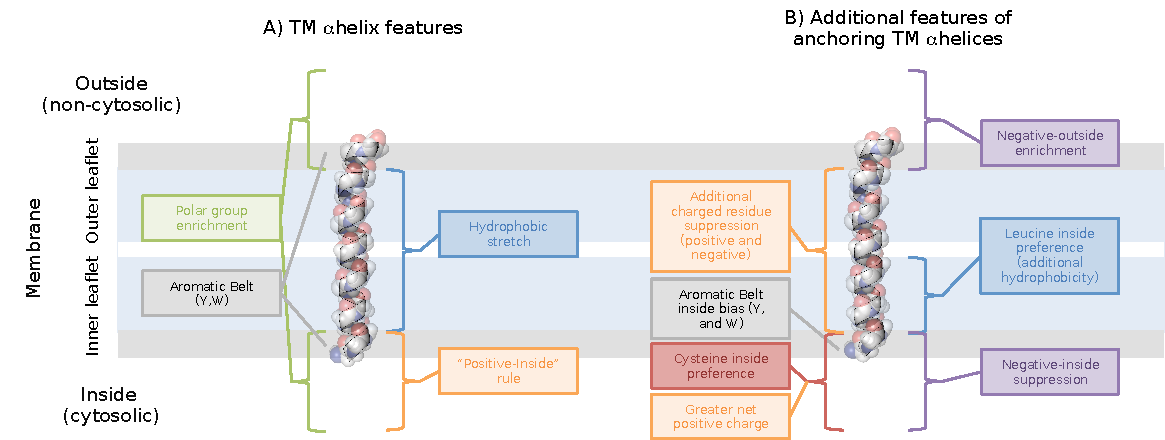
\includegraphics[width=1\textwidth]{NNI_chapter/overview}
\captionof{figure}[Residue distributions of transmembrane anchors.
A view showing additional residue distribution features that~\gls{tmh}s with an anchorage function display.]{\textbf{Residue distributions of transmembrane anchors.
A view showing additional residue distribution features that~\gls{tmh}s with an anchorage function display.}a The more classic model of a~\gls{tmh} showing the ``positive-inside'' rule~\cite{VonHeijne1989}, the hydrophobic core~\cite{Kyte1982}, the polar enrichment that flanks the hydrophobic stretch~\cite{Baeza-Delgado2013} and the aromatic belt~\cite{Granseth2005}.
b Simple anchors may display additional features that conform to the membrane biophysical constraints: further suppression of charge in the hydrophobic core (Table \ref{table:acidicresiduesarerare}), intra-membrane leucine asymmetry that likely causes hydrophobic skew~\cite{Sharpe2010} (Table~\ref{table:leucineskewstats}, Figure~\ref{fig:hydrophobicity_single_multi}), a higher preference for cysteine on the inside flanking region (Figure~\ref{fig:complexity_datasets}K and L), a higher net ``positive-inside'' charge (Figure~\ref{fig:net_charge}), asymmetric skew of the hydrophobic belt favouring the inner leaflet interface (Figure~\ref{fig:complexity_datasets}E, F, G, and H) and a negative-outside bias via suppression on the inside flanking region or enrichment on the outside flanking region (Figure~\ref{fig:complexity_datasets}C and D, Tables 2 and 3)}

\label{fig:overview}
\end{figure}

In summary, three key features can be assigned to aiding~\gls{tmh} stability in the membrane (Figure~\ref{fig:overview}): (i) charge, (ii) the aromatic belt, and (iii) leucine leaflet preference.
What is most novel here is that each of these features are furthermore distributed with preference for a particular side of the bilayer in the case of anchoring~\gls{tmh}s.
These differences in inside-outside topology that are most present in anchoring~\gls{tmh}s further supports the notion that there are broad lipid compositional differences between the inner and outer leaflets of the bilayers~\cite{Sharpe2010}.
Furthermore, while some~\gls{tmh}s conform and complement to the properties of the bilayer, other~\gls{tmh}s with function beyond anchorage are less constrained to biophysically complement the bilayer.
For these~\gls{tmh}s, any advantage gained by adhering to the membrane restrictions is outweighed by more complicated protein dynamics, topological frustration and protein functional requirements.

To conclude, the large fraction of functionally uncharacterised genomic sequences is the great bottleneck in life sciences at this moment that hinders many biomedical and biotechnological applications, some with tremendous societal need~\cite{Eisenhaber2012,Kuznetsov2013}.
Among these uncharacterised genomic regions, there is \(\sim\)10000 protein-coding genes, especially many membrane-embedded proteins.
It is hoped that the NNI/NO-rule as well as the other sequence properties of membrane anchoring~\gls{tmh}s described in this article will add new insights for membrane protein function discovery, design and engineering.

\section{Methods}

\subsection{Datasets}
\subsubsection{Databases.}
All datasets used for analysis are listed in Table \ref{table:acidicresiduesarerare}.
Transmembrane protein sequences and annotations were taken from TOPDB~\cite{Dobson2015} and UniProt~\cite{TheUniProtConsortium2014}.
UniProt derived datasets are the most comprehensive datasets built with (i) robust transmembrane prediction methods providing the limit of today’s achievable accuracy with regard to hydrophobic core localisation and (ii) subcellular location annotation that can be used for orientation determination.
However, they mostly rely on predicted transmembrane regions.
TOPDB has meticulous experimental verifications of the orientation from the literature that are independent of prediction algorithms~\cite{Dobson2015}.
Unfortunately, this dataset is much smaller with too few entries to have it divided with regard to taxonomy or subcellular locations.

UniProt database files were downloaded by querying the server for different taxonomic groups as well as different subcellular membrane locations; UniHuman (human representative proteome), UniCress (Arabidopsis thaliana, otherwise known as mouse eared cress, representative proteome), UniER (human endoplasmic reticulum representative proteome), UniPM (human plasma membrane representative proteome), UniGolgi (human Golgi representative proteome).
To enforce a level of quality control, the queries were restricted to manually reviewed records and transmembrane proteins with manually asserted TRANSMEM annotation~\cite{TheUniProtConsortium2014}.
Proteins were then sorted into multi-pass and single-pass groups according to having more than one or exactly one TRANSMEM region respectively.
TRANSMEM regions are validated by either experimental evidence~\cite{TheUniProtConsortium2014}, or according to a robust transmembrane consensus of the predictors TMHMM~\cite{Krogh2001}, Memsat~\cite{Jones2007}, Phobius~\cite{Kall2004,Kall2007} and the hydrophobic moment plot method of Eisenberg and co-workers~\cite{Eisenberg1984}.
\gls{tmh}s and flanking regions were oriented according to UniProt TOPO\_DOM annotation according to the keyword ``cytoplasmic''.
If a ``cytoplasmic'' TOPO\_DOM was found in the previous TOPO\_DOM relative to the TRANSMEM region then the sequence remained the same.
If ``cytoplasmic'' was found in the next TOPO\_DOM, relative to the TRANSMEM section then the sequence was reversed.
Proteins without the ``cytoplasmic'' keyword in their TOPO\_DOM annotation were omitted from further analysis.

The TOPDB database~\cite{Dobson2015} is a manually curated database composed of experimental records from the literature that allow determination of the protein topology.
Experiments include fusion proteins, posttranslational modifications, protease experiments, immunolocalization, chemical modifications as well as revertants, sequence motifs with known mandatory membrane-embedded topologies, and tailoring mutants (Table~\ref{table:topdbevidence}).

\begin{table}[htbp]
  \tiny
  \centering

  \captionof{table}[The experimental evidences of TOPDB.]{\textbf{The experimental evidences of TOPDB.}
  The total number of experimental evidences that contribute to ExpAll according to the TOPDB database (More information at \url{http://topdb.enzim.hu/?m=exptype&mid=14}).
  ``*'' refers to the total number of a subsection being larger than the total of the subcategories, likely due to lack of annotation where ambiguous literature evidence is counted toward the total, but cannot be categorised further.}
    \resizebox{\textwidth}{!}{
    \begin{tabular}{cp{5em}cp{5em}}
    \toprule
    \multicolumn{2}{p{10em}}{\textbf{Experiment}} & \multicolumn{1}{p{5em}}{\textbf{Bitopic (Single-pass)}} & \textbf{Polytopic (Multi-pass)} \\
    \midrule
    \multicolumn{1}{c}{\multirow{13}[26]{*}{\textbf{Fusion}}} & PhoA  & 97    & \multicolumn{1}{c}{2332} \\
    \cmidrule{2-4}          & PhoAS & 0     & \multicolumn{1}{c}{90} \\
    \cmidrule{2-4}          & LacZ  & 20    & \multicolumn{1}{c}{433} \\
    \cmidrule{2-4}          & PhoALacZ & 0     & \multicolumn{1}{c}{224} \\
    \cmidrule{2-4}          & BlaM  & 162   & \multicolumn{1}{c}{570} \\
    \cmidrule{2-4}          & BAD   & 0     & \multicolumn{1}{c}{2} \\
    \cmidrule{2-4}          & PL    & 0     & \multicolumn{1}{c}{47} \\
    \cmidrule{2-4}          & GFP   & 18    & \multicolumn{1}{c}{591} \\
    \cmidrule{2-4}          & HIS   & 4     & \multicolumn{1}{c}{2} \\
    \cmidrule{2-4}          & SplitUbiquitin & 0     & \multicolumn{1}{c}{11} \\
    \cmidrule{2-4}          & Suc2  & 0     & \multicolumn{1}{c}{96} \\
    \cmidrule{2-4}          & Other & 1     & \multicolumn{1}{c}{137} \\
    \cmidrule{2-4}          & Total Fusion & \multicolumn{1}{p{5em}}{316*} & 4600* \\
    \midrule
    \multicolumn{1}{c}{\multirow{5}[10]{*}{\textbf{PostTransMod}}} & NGlyc & 4634  & \multicolumn{1}{c}{1130} \\
\cmidrule{2-4}          & Cman  & 0     & \multicolumn{1}{c}{6} \\
\cmidrule{2-4}          & Phosphorylation & 4     & \multicolumn{1}{c}{1} \\
\cmidrule{2-4}          & Ubiquitination & 47    & \multicolumn{1}{c}{102} \\
\cmidrule{2-4}          & Total PostTransMod & 4685  & \multicolumn{1}{c}{1239} \\
    \midrule
    \multicolumn{1}{c}{\multirow{4}[8]{*}{\textbf{Protease}}} & Partial Proteolysis & 51    & \multicolumn{1}{c}{264} \\
\cmidrule{2-4}          & Signal Peptidase & 1     & \multicolumn{1}{c}{0} \\
\cmidrule{2-4}          & TID   & 13    & \multicolumn{1}{c}{15} \\
\cmidrule{2-4}          & Total Protease & 64    & \multicolumn{1}{c}{279} \\
    \midrule
    \multicolumn{1}{c}{\multirow{3}[6]{*}{\textbf{Immunolocalisation}}} & Epitope Insertion & 33    & \multicolumn{1}{c}{313} \\
\cmidrule{2-4}          & Endogen Epitope & 8     & \multicolumn{1}{c}{41} \\
\cmidrule{2-4}          & Total Immunolocalisation & \multicolumn{1}{p{5em}}{53*} & 451* \\
    \midrule
    \multicolumn{1}{c}{\multirow{4}[8]{*}{\textbf{Chemical modification}}} & Cys   & 0     & \multicolumn{1}{c}{361} \\
\cmidrule{2-4}          & Lys   & 0     & \multicolumn{1}{c}{3} \\
\cmidrule{2-4}          & Quenching & 0     & \multicolumn{1}{c}{2} \\
\cmidrule{2-4}          & Total Chemical Modification & 0     & 368* \\
    \midrule
    \multicolumn{1}{p{5em}}{\textbf{Structure}} & PDBTM TMDET & 5968  & \multicolumn{1}{c}{41977} \\
    \midrule
    \multicolumn{1}{c}{\multirow{4}[8]{*}{\textbf{Other}}} & Revertants & 0     & \multicolumn{1}{c}{14} \\
\cmidrule{2-4}          & SeqMotif & 2     & \multicolumn{1}{c}{32} \\
\cmidrule{2-4}          & Tailoring & 1     & \multicolumn{1}{c}{67} \\
\cmidrule{2-4}          & Total other & 3     & 115* \\
    \bottomrule
    \end{tabular}%
    }
   \label{table:topdbevidence}

\end{table}%

Length cut-offs for the~\gls{tmh} were set at 16 as the shortest length and 38 as the longest.

To note, we are aware that proteome datasets are a moving target that have dramatically changed over the years and, probably, will continue to do so to some extent in the future[83].
Yet, we think that currently available protein sequence sets are sufficiently good for the purpose as we search for statistical properties in the~\gls{tmh} context only.

The following datasets are used throughout this work:

\subsubsection{ExpAll}

TOPDB contained 4190 manually annotated transmembrane proteins at the time of download~\cite{Dobson2015}.
CD-HIT~\cite{Huang2010} identified 3857 representative sequences using sequence clusters of $>$90\% sequence identity.
This choice of similarity threshold was chosen since CD-HIT ultimately underlies the clustering behind UniRef.
Unlike the other datasets, which by definition contain reasonably typical~\gls{tmh}s, many of the transmembrane segments annotated in TOPDB are extremely short or long and this would cause severe unrealistic hydrophobic mismatches.
Especially, the short segments could be the result of miss-annotation,~\gls{tmh}s broken into pieces due to kinks or segments that peripherally insert only into the interface of the membrane bilayer.
To remove the atypical lengths, cut-offs were set at 16 as the lower cut-off and 38 as the upper cut-off after inspecting the length histogram.
We found that, for the single-pass~\gls{tmh}s in TOPDB, 1215 out of 1544 are within the length limits (78.7\%).
Among the 17141 multi-pass~\gls{tmh}s, we find 15563 within our global length limits (from 2205 TOPDB records corresponding to 2281 UniProt entries).
This removed 1578 very short~\gls{tmh}s and none of the long~\gls{tmh}s.
Our cut-off selection is very similar to the one by Baeza-Delgado \textit{et al.}~\cite{Baeza-Delgado2013}.

To get an idea of the taxonomical breakdown in the ExpAll dataset, the UniProt ID tags were extracted and mapped to UniProtKB.
The combined dataset of multi-pass (single-pass) proteins was mapped to 1288 (1343) eukaryotic records, 404 (776) of which were human records, 926 (191) bacterial records, 46 (5) archaea records, and 14 (22) viral records.


\subsubsection{UniHuman}
This is a set of mostly human~\gls{tmh}-containing proteins or their close mammalian homologues.
UniProtKB contains 5187 human protein records that are manually annotated with TRANSMEM regions (query = ``annotation:(type:transmem) AND reviewed:yes AND organism:``Homo sapiens (Human) [9606]'' AND proteome:up000005640''.
To reduce sequence redundancy, these sequences were submitted to UniRef90~\cite{Suzek2015}.
To note, UniRef90 was chosen over UniRef50 to maintain a viable size of datasets for statistical analysis of occurrence of negatively charged residue, which are very rare in the vicinity of~\gls{tmh}s.
5015 UniRef90 clusters represented the 5187 sequences.
A list of sequences representing those clusters was submitted back to UniProtKB resulting and 5014 representative entries were recovered.
There is a small issue in that the list of representatives from UniRef includes non-canonical isoforms, while the batch retrieve query of UniProtKB only supports complete entries, i.e.
canonical isoforms.
This resulted in the loss of one record at this point is due to two splice isoforms acting as representative identifiers.
Of those 5014 records, 4714 were records from human entries, 197 were from mice, 94 from rats, 5 from bovine, 2 from chimps, 1 from Chinese hamsters, and 1 from pigs.
Although the~\gls{tmh} length variations within the UniHuman dataset are much smaller than for ExpAll, we applied the same length cut-offs for the sake of comparability.
Out of the 1709 single-pass cases, 1705 entered the final dataset.
Of those, 1596 were from human records, 87 were from mouse, 19 were from rat, and 2 were from chimpanzee.
Among the 12390 multi-pass~\gls{tmh}s, 12353 were included into UniHuman.
The other, multi-pass record identifiers were mapped to 1789 UniProtKB entries.
1660 of these were human entries, 63 from rat, 61 from mouse, 4 from bovine, and 1 from Chinese hamster.
This clustered human dataset was then queried for subcellular locations to make the UniER, UniGolgi, and UniPM datasets (detailed below).

\subsubsection{UniER}
The clustered UniHuman dataset was queried using UniProtKB for endoplasmic reticulum subcellular location (locations:(location:``Endoplasmic reticulum [SL-0095]'' evidence:manual)).
This returned 487 protein entries, 457 of which belonged to human, 24 to mouse and 6 to rat.
287 of these records contained sufficient annotation for orientation determination.
132 were single-pass entries of which 120 records were from humans, 11 from mouse, and 1 from rat.
155 were multi-pass entries containing 898 transmembrane helices.
144 were records from human, 8 were from mouse and 3 were from rat.

\subsubsection{UniGolgi}
The clustered human dataset was queried using UniProtKB for Golgi subcellular location (locations:(location:``Golgi apparatus [SL-0132]'' evidence:manual)).
This returned 323 protein entries, 301 of which belonged to human, 19 to mice, 2 to rat and 1 to pig.
269 of these records contained sufficient annotation for orientation determination.
206 were single-pass entries of which 195 records were from human, 9 from mouse, and 1 from rat.
61 were multi-pass entries containing 383 transmembrane regions.
54 were records from human, 6 were from mouse and 1 was from rat.

\subsubsection{UniPM}
The clustered human dataset was queried using UniProtKB for the cell membrane subcellular location (locations:(location:``Cell membrane [SL-0039]'' evidence:manual)).
This returned 1036 protein entries, 948 of which belonged to humans, 62 to mice, and 26 to rats.
920 of these records contained sufficient annotation for orientation determination.
493 were single-pass entries of which 451 records were from human, 37 from mouse, and 5 from rat.
427 were multi-pass entries containing 3079 transmembrane regions.
394 were records from human, 17 were from mouse and 16 were from rat.

\subsubsection{UniCress}
For the mouse ear cress, a representative proteome dataset was acquired with the query annotation:proteomes:(reference:yes) AND reviewed:yes AND organism:``Arabidopsis thaliana (Mouse-ear cress) [3702]'' AND proteome:up000006548.
This returned 3174 records in UniProtKB.
UniRef90 identified 3111 clusters.
3110 of the representative sequences were mapped back to UniProtKB.
Of those, 3090 were from Arabidopsis thaliana, 2 from Hornwort, 1 from cucumber, 1 from tall dodder, 1 from soybean (Glycine max), 2 from Indian wild rice, 2 from rice, 2 from garden pea, 1 from potato, 4 from spinach, 1 from Thermosynechococcus elongatus (thermophilic cyanobacteria), 1 from wheat, and 2 from maize.
Of those there were 1146 with suitable TOPO\textunderscore DOM annotation for topological orientation determination.
632 of those records were identified as single-pass, all of which were from Arabidopsis thaliana.
507 protein records were from multi-pass records, which contained 3823 transmembrane helices.
506 of those records were from Arabidopsis thaliana, whilst 1 was from Thermosynechococcus elongatus.

\subsubsection{UniFungi}
For the Fungi dataset, the query ``annotation:(type:transmem) taxonomy:``Fungi [4751]'' AND reviewed:yes'' was used.
This returned 5628 records that were submitted to UniRef90.
UniRef90 identified 4934 representative records, all of which were successfully mapped back to UniProtKB.
Of those, 2070 had suitable annotation for orientation.
1990 records belonged to Ascomycota including 1243 Saccharomycetales.
73 were Basidomycota, and 6 were Apansporoblastina.
729 records contained a single~\gls{tmh} region, 702 of which belonged to Ascomycota, 26 to Basidomycota and one to Encephalitozoon cuniculi, a Microsporidium parasite.
8698 helices were contained in 1338 records of multi-pass proteins.
Of these records 1285 were Ascomycota, 47 were Basidomycota, and 5 were Apansporoblastina.
One~\gls{tmh} from UniFungi was discounted from P32897 due to an unknown position.

\subsubsection{UniEcoli}
This dataset was generated by querying UniProt with ``reviewed:yes AND organism:''Escherichia coli (strain K12)[83333]'''' which returned 941 hits.
The hits were submitted to UniRef90, which returned 935 clusters.
The representative IDs were then resubmitted to UniProtKB, all of which returned successfully.
934 were from Bacteria, whilst one were from lambdalike viruses.
Of the bacterial records, 862 were from various Escherichia species of which 565 were from E.
coli strain K12, 28 were from Salmonella choleraesuis, 25 were from Shigella and the rest all also fell under Gammaproteobacteria class.
This dataset contains 54 single-pass proteins and 3888 helices from 529 multi-pass proteins with sufficient annotation for topological determination.

\subsubsection{UniBacilli}
The Bacilli dataset was constructed by querying UniProt for ``reviewed:yes AND taxonomy:''Bacilli''''.
This returned 5044 records, which were submitted to UniRef90.
2,591 clusters were found in UniRef from these records.
The representative IDs were successfully resubmitted to UniProtKB.
2031 of these were of the genus Bacillales whilst 560 were also of the genus Lactobacillales.
This dataset contains 124 single-pass proteins and 822 helices from 140 multi-pass proteins.

\subsubsection{UniArch}
The Archaea dataset was constructed by querying UniProt for ``reviewed:yes AND taxonomy:''Archaea [2157]''''.
This returned 1,152 records, which were submitted to UniRef90.
1,054 clusters were found in UniRef from these records.
The representative IDs were successfully resubmitted to UniProtKB.
946 records belonged to the Euyarchaeota, 101 to Thermoprotei, 4 to Thaumarchaeota, and 3 to Korarchaeum cryptofilum.
This dataset contains 48 single-pass proteins and 59 multi-pass proteins containing 327 helices from 59 proteins.


\subsection{On the determination of flanking regions for~\gls{tmh}s and the~\gls{tmh} alignment}

The determination of the boundary point at the sequence between the~\gls{tmh} in a membrane and the sequence immersed in the cytoplasm, extracellular space, vesicular lumen, etc.
is not that trivial as it initially appears.
There is a lot of dynamics in the~\gls{tmh} positioning and the actual boundary point will be represented by various residues at different time points.
Whilst the~\gls{tmh} core region detection from a sequence is trivial with modern software, the exact determination of~\gls{tmh} boundaries remains difficult since it is unclear exactly how far in or out of the membrane a given helix extends~\cite{Ojemalm2013}.
Previous studies have dealt with this issue in various ways~\cite{Sharpe2010,Baeza-Delgado2013,Pogozheva2013, White2008}.

Here in this work, we explore two boundary definitions.
First, we assign~\gls{tmh} boundary locations as described in the respective databases.
These flanks are the ones that are reported in our~\gls{tmh} data files that are available at the WWW-site associated with this paper.
We studied flank lengths of $\pm$5, $\pm$10, and $\pm$20 residues preceding and following the inside and outside~\gls{tmh} boundaries.
In these cases, the flanks are aligned relative to the residue closest to the~\gls{tmh}.

In cases where the loops before and after the~\gls{tmh} are shorter than the predefined flank lengths, further precautions are necessary.
In the multi-pass datasets particularly (Figure~\ref{fig:flank_definitions} \& Figure~\ref{fig:net_charge}), the flanks overlap with other membrane region flanks.
We explore several variants.
On the one hand, we work with data files where the flank residue stretches are equally truncated so that no overlap occurs.
If the loop length was uneven, the central odd residue was not included into any flank.
We find surprisingly, that a large number of~\gls{tmh} has no or just a super-short flank, a circumstance that should disturb any statistical analysis due to the absence of objects.
Therefore, we also work with alternative datasets (i) with flanks overlapping between consecutive~\gls{tmh} (e.g., in Table 3B; yet, it leads to some residues being counted more than one time) as well as (ii) with subsets of the data where the flanks at both sides have a defined minimal length (50\% or 100\% of the required flanks; unfortunately, some of them become too small for analysis).

\begin{figure}[!ht]
\centering
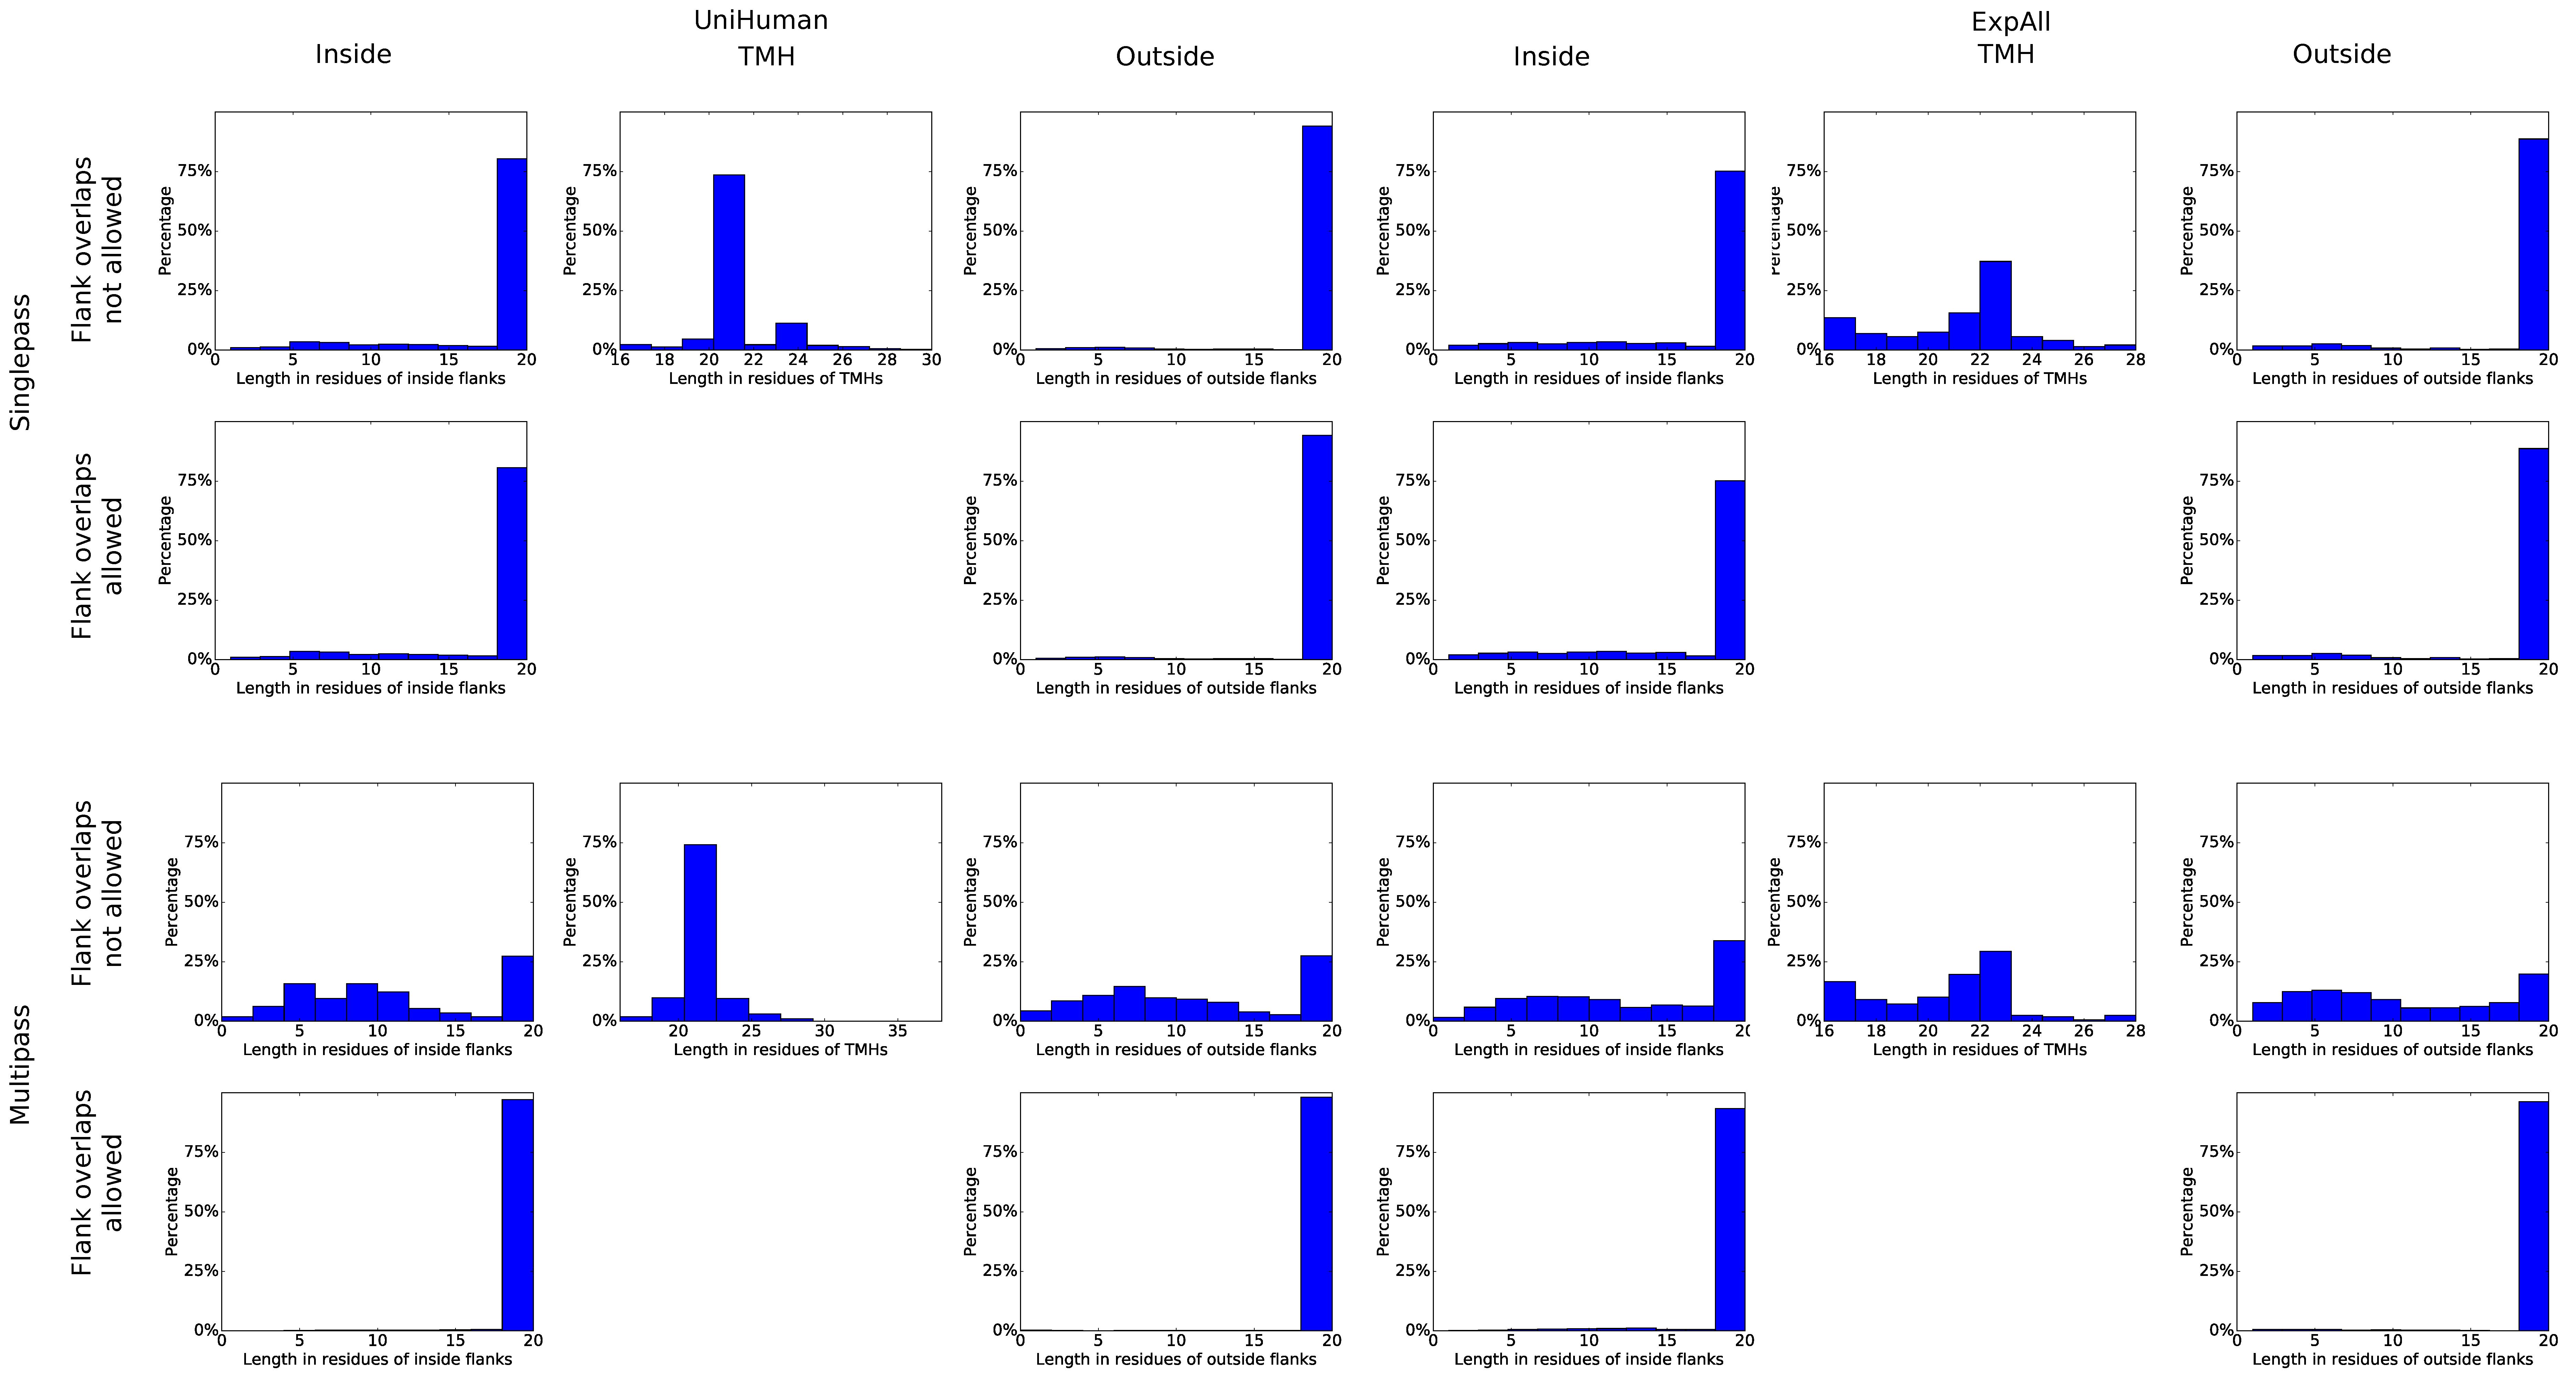
\includegraphics[width=1\textwidth]{NNI_chapter/flank_definitions}
\captionof{figure}[The lengths of flanks and~\gls{tmh}s in multi-pass and single-pass proteins in the UniHuman and ExpAll dataset.]{\textbf{The lengths of flanks and~\gls{tmh}s in multi-pass and single-pass proteins in the UniHuman and ExpAll dataset.}On the horizontal axis are the lengths of the~\gls{tm} segment regions in residues.
On the vertical axis are the percentages of the population.
There are three regions: the inside flank, the~\gls{tmh} and the outside flank.
These regions are acquired according to the~\gls{tmh} boundary of the respective database.
Where no overlap is permitted, if the flank encroaches the flank of another~\gls{tmh}, the flank length becomes half the number of residues in the loop region between the two features.
Where they are allowed to overlap, flanking residues may include other flanks, or indeed other~\gls{tmh}s.}

\label{fig:flank_definitions}
\end{figure}

The problem of flanks overlapping does affect also some single-pass and multi-pass~\gls{tmh} proteins with INTRAMEM regions as described in some UniProt entries.
We do not include INTRAMEM regions in the datasets as~\gls{tmh}s but, sometimes, the flanking regions of~\gls{tmh}s were truncated to avoid overlap with INTRAMEM flanking regions (Supplementary Table S2).
 The identifiers affected for single-pass~\gls{tmh} proteins are Q01628, P13164, Q01629, Q5JRA8, A2ANU3 (UniHuman), P13164, Q01629, A2ANU3 (UniPM) and Q5JRA8 (UniER).

 \begin{table}[htbp]

   \centering

   \captionof{table}[Records with INTRAMEM and TRANSMEM flanking region overlap.]{\textbf{Records with INTRAMEM and TRANSMEM flanking region overlap.}
   The total number of TMHs from UniProt datasets with flanking region overlap between INTRAMEM and TRANSMEM regions.
   The number of multi-pass records that the TMHs belong to are shown in brackets.}
     \resizebox{\textwidth}{!}{
     \begin{tabular}{p{5em}cccp{5em}cp{5em}}
     \toprule
     \multirow{3}[6]{*}{\textbf{Dataset}} & \multicolumn{6}{p{30em}}{\textbf{Flank length}} \\
     \cmidrule{2-7}    \multicolumn{1}{c}{} & \multicolumn{2}{c}{\textbf{5}} & \multicolumn{2}{c}{\textbf{10}} & \multicolumn{2}{c}{\textbf{20}} \\
     \cmidrule{2-7}    \multicolumn{1}{c}{} & \multicolumn{1}{p{5em}}{\textbf{Single-pass}} & \multicolumn{1}{p{5em}}{\textbf{Multi-pass}} & \multicolumn{1}{p{5em}}{\textbf{Single-pass}} & \textbf{Multi-pass} & \multicolumn{1}{p{5em}}{\textbf{Single-pass}} & \textbf{Multi-pass} \\
     \midrule
     \textbf{UniHuman} & 0     & \multicolumn{1}{c}{96 (80)} & 1     & 151 (90) & 5     & 204 (96) \\
     \midrule
     \textbf{UniER} & 0     & \multicolumn{1}{c}{6 (6)} & 1     & 13 (8) & 1     & 16 (8) \\
     \midrule
     \textbf{UniGolgi} & 0     & \multicolumn{1}{c}{1 (1)} & 0     & 2 (2) & 0     & 4 (2) \\
     \midrule
     \textbf{UniPM} & 0     & \multicolumn{1}{c}{57 (46)} & 0     & 93 (51) & 3     & 113 (52) \\
     \midrule
     \textbf{UniCress} & 0     & \multicolumn{1}{c}{17 (17)} & 0     & 24 (18) & 0     & 46 (18) \\
     \midrule
     \textbf{UniFungi} & 0     & 0     & 0     & \multicolumn{1}{c}{0} & 0     & \multicolumn{1}{c}{0} \\
     \midrule
     \textbf{UniBacilli} & 0     & \multicolumn{1}{c}{11 (3)} & 0     & 12 (3) & 0     & 13 (3) \\
     \midrule
     \textbf{UniEcoli} & 0     & \multicolumn{1}{c}{22 (8)} & 0     & 25 (9) & 0     & 31 (9) \\
     \midrule
     \textbf{UniArch} & 0     & 0     & 0     & 8 (8) & 0     & 17 (9) \\
     \bottomrule
     \end{tabular}%
     }
    \label{table:overlapflankingregions}

 \end{table}%


The second form of boundary point definition for flank determination was achieved with gaplessly aligning all~\gls{tmh}s relative to their central residue at the position equal to half the length of the~\gls{tmh}s at either side.
Though there is some length variation among~\gls{tmh}s, most of them are centred around a length of 20-22 residues.
In this case, flanks are the sequence extensions beyond the standardised-length 21-residues~\gls{tmh}s.
We define the inside flanking segments as the positions -20 to -10 and the outside flanking regions to be +10 to +20 from the central~\gls{tmh} residue (with the label ``0'').
Instead of emphasising some artificially selected boundary residue, this definition allows the average~\gls{tmh} boundary transition to become apparent.

\subsection{Separating simple and complex single-pass helices.}

Single-pass helices from ExpAll and UniHuman datasets helices were split into two groups: simple and complex following a previously described classification~\cite{Wong2011,Wong2012} to roughly distinguish simple hydrophobic anchors and~\gls{tmh}s with additional structural/functional roles.
Simple and complex helices were determined using TMSOC~\cite{Wong2012}.
The complexity class is determined by calculating the hydrophobicity and sequence entropy.
The resulting coordinates cluster with anchors being more hydrophobic and less complex whilst more complex and more polar~\gls{tmh}s are associated with non-anchorage functions.
In UniHuman there were 889 simple helices and 570 complex~\gls{tmh}s.
In ExpAll there were 769 simple helices and 570 complex helices.

\subsection{Distribution normalisation}

In this work, we have used normalisation techniques described in previous investigations as well as new approaches designed to more sensitively identify biases of rare residues.
Baeza-Delgado and co-workers used LogOdds normalisation column-wise in~\gls{tmh} alignments.
Critically, this is based on their definition of probability, which takes into account the total number of amino acids in the dataset as a denominator~\cite{Baeza-Delgado2013}.
Since aliphatic residues such as leucine and other highly abundant slightly polar residues dominate the denominator, the distribution of the rare acidic residues will be easily lost in the ``background noise'' of those highly abundant residues.
Pogozheva and co-workers used two approaches, (i) the total accessible surface area (ASAtotal) and (ii) total number of charged residues (${N}_{total}$) as a denominator in their distribution normalisation~\cite{Pogozheva2013}.

In this work, two methods for measuring residue occurrence in the~\gls{tmh} and its flanks were used.
Similarly to previous work, we compute the occurrence  of an amino acid type  at a certain sequence position  in a set of aligned sequences~\gls{tmh}s and their flanks.
Following~\cite{Sharpe2010}, the absolute relative occurrence  of this amino acid type at the sequence position  is then given by Equation~\ref{eq:dependent_normalisation} as:

\begin{equation} \label{eq:dependent_normalisation}
  p_{i,r}=\frac{a_{i,r}}{\underset{r}{\max}{(a_r)}}
\end{equation}


Here, the denominator is the maximal number of all residues in any alignment column (i.e., the number of sequences in the alignment) and, to emphasise, this will make  mostly dependent on the most abundant residue types.
This type of normalisation reveals the most preferred residue types at given sequence positions.

Our second normalisation method is independent of the abundance of any amino acid types other than the studied one; it answers the question: ``If there is a residue of type  in the~\gls{tmh}-containing segment, where would it most likely be?'' This relative occurrence  calculated in Equation~\ref{eq:independent_normalisation} as:

 \begin{equation} \label{eq:independent_normalisation}
   q_{i,r}=\frac{{100}\cdot{a_{i,r}}}{a_i}
 \end{equation}

The value $a_i$ is the total abundance of residues of just amino acid type $i$ in a given alignment of~\gls{tmh}-containing segments (i.e., in the~\gls{tmh} together with its two adjoining flanks summed over all cases of~\gls{tmh}s in the given dataset).
Peaks in $q_{i,r}$ as function of $r$ reveal the preferred positions of residues of type $i$.
The difference in $q_{i,r}$ and $p_{i,r}$ normalisation is visualised in Figure~\ref{fig:normalisation}.

\begin{figure}[!ht]
\centering
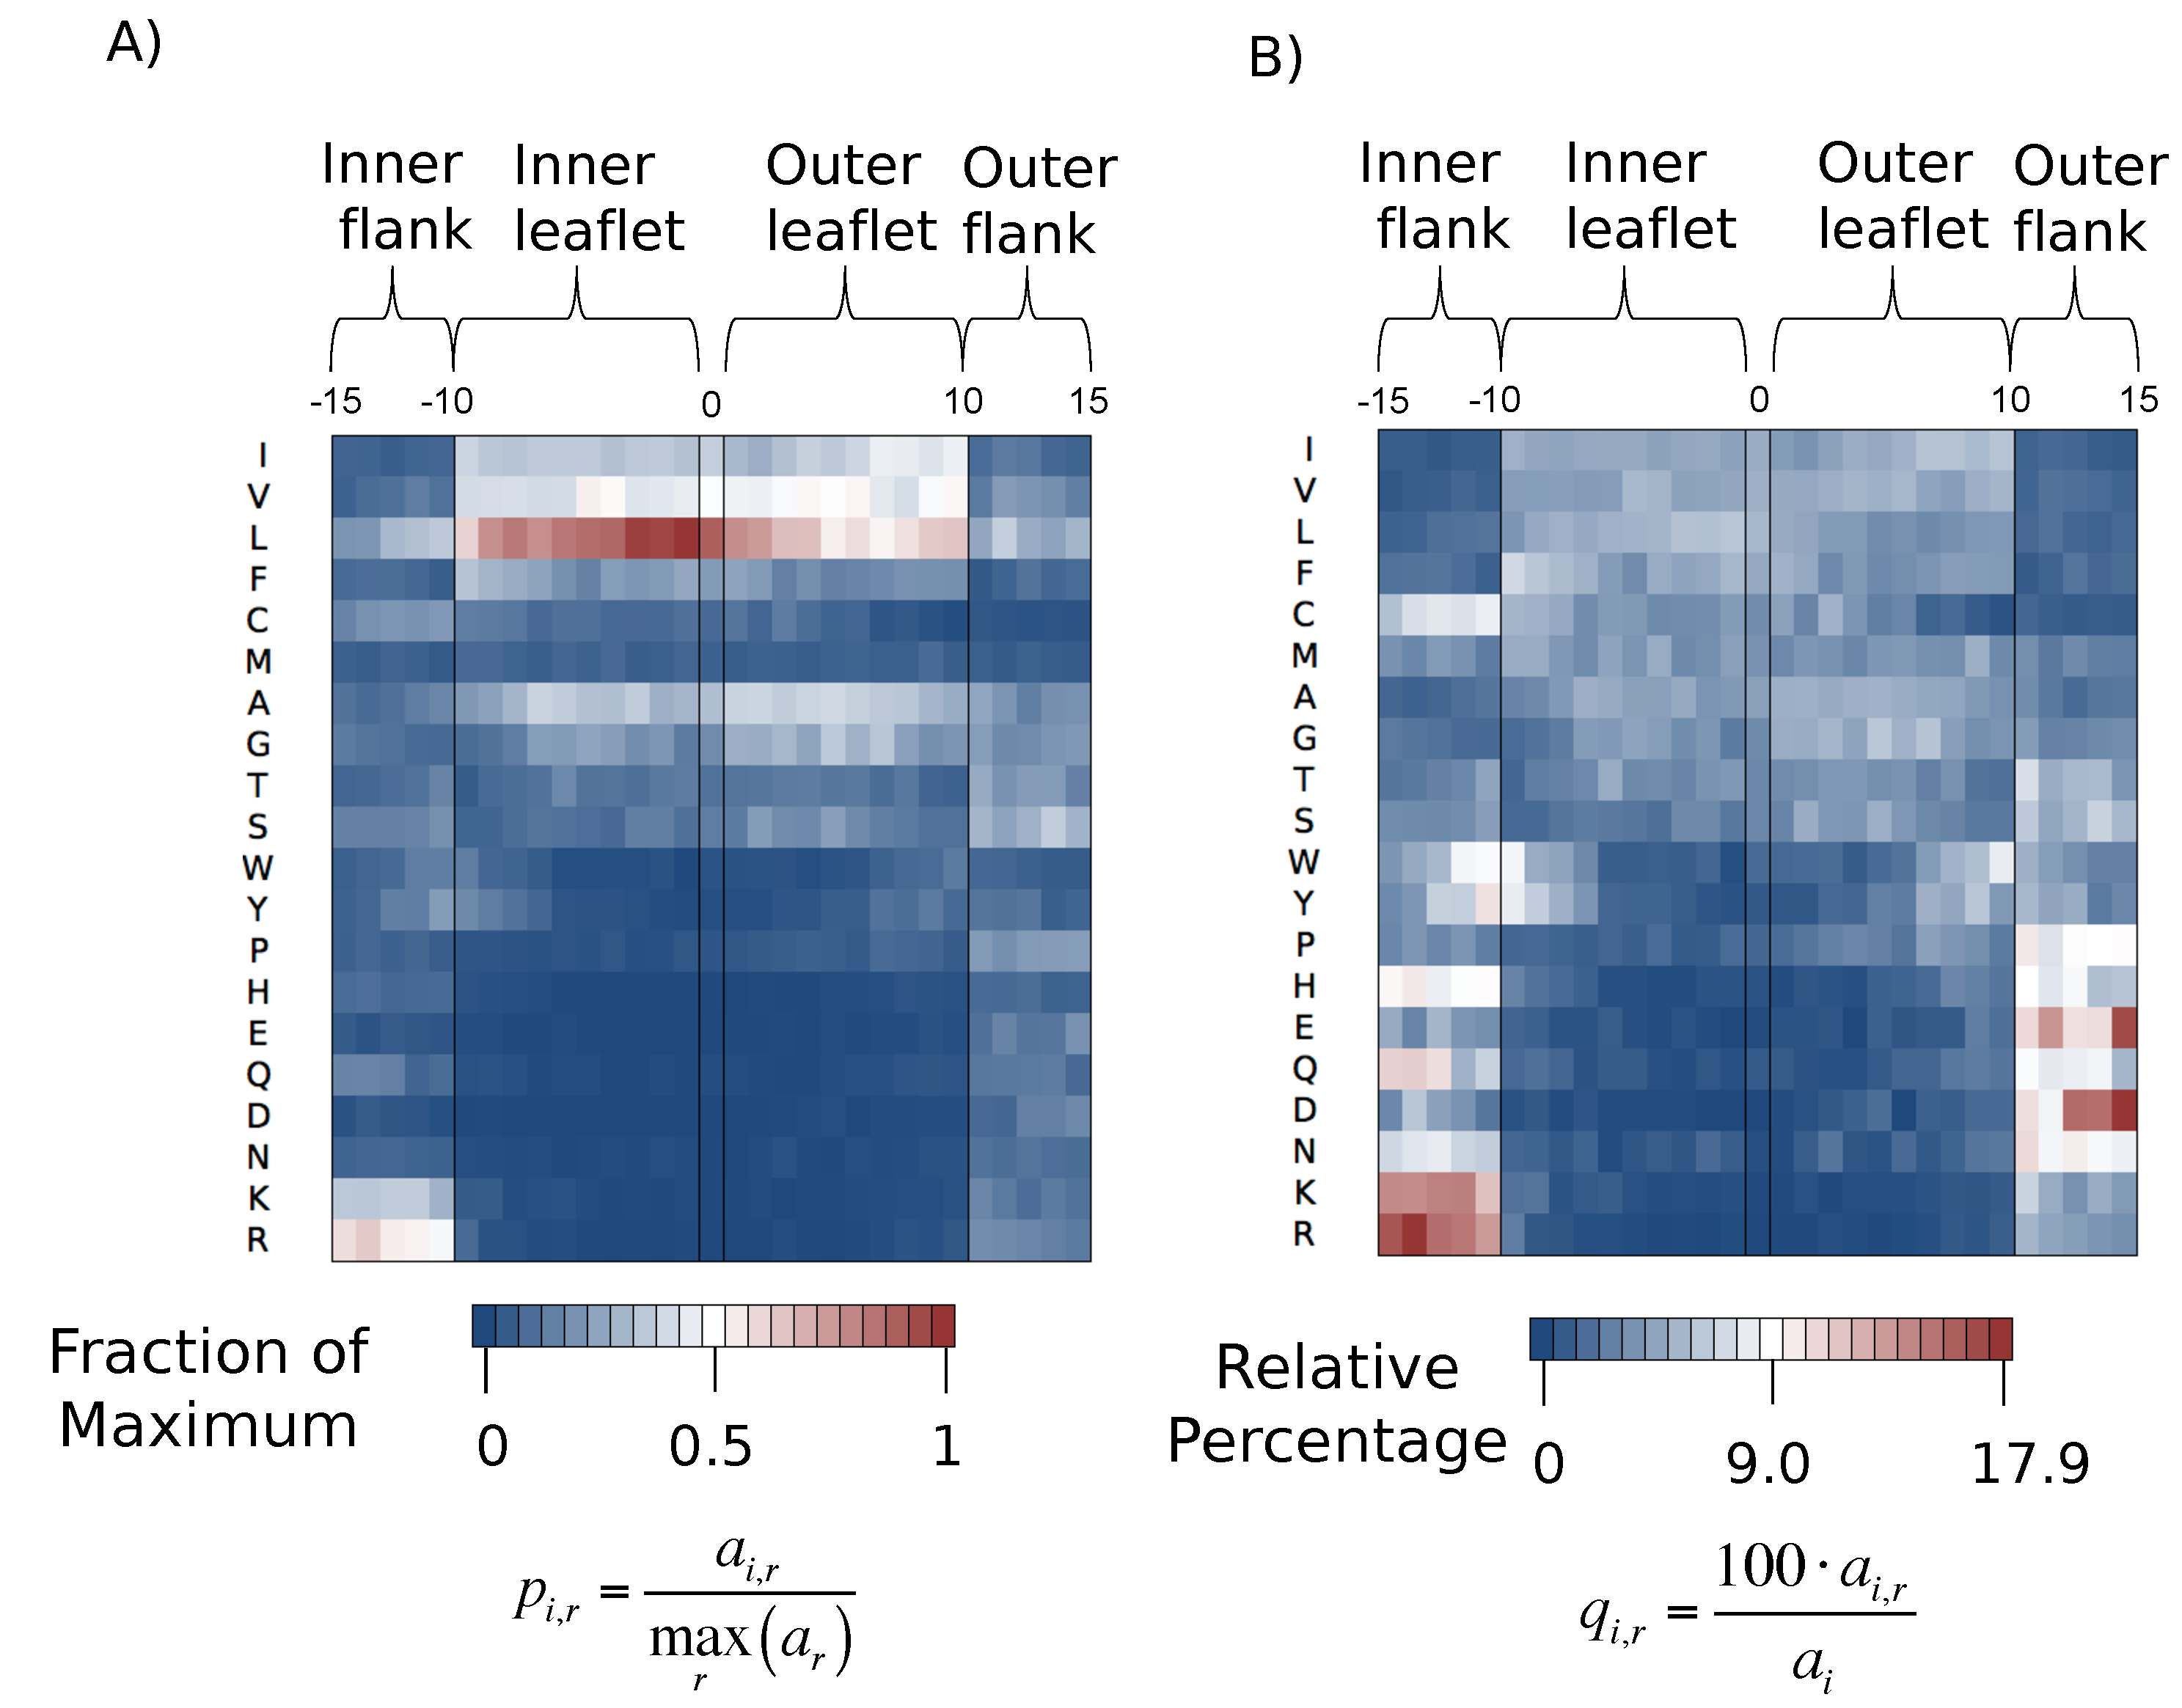
\includegraphics[width=1\textwidth]{NNI_chapter/normalisation}
\captionof{figure}[Relative percentage heatmaps from the predictive datasets calculated by fractions of the absolute maximum and by the relative percentage of a given amino acid type.]{\textbf{Relative percentage heatmaps from the predictive datasets calculated by fractions of the absolute maximum and by the relative percentage of a given amino acid type.}The residue position aligned to the centre of the~\gls{tmh} is on the horizontal axis, and the residue type is on the vertical axis.
Amino acid types are listed in order of decreasing hydrophobicity according to the Kyte and Doolittle scale~\cite{Kyte1982}.
The flank lengths in the~\gls{tmh} segments were restricted to up to $\pm$5 residues.
The scales for each heatmap are shown beneath the respective subfigure.
All~\gls{tmh}s and flank lengths are from the UniHuman dataset.
(A) The heatmap has been coloured according to a scale that uses column-wise normalisations used in previous studies~\cite{Sharpe2010}.
See Equation~\ref{eq:dependent_normalisation}.
As an illustrative example, we show how the value for E at position $\pm$12 is obtained.
There are in total 91/22 Es at these positions in 1705 sequences; thus, the represented value is 0.013 at –12 and 0.053 at 12.
Note that L is clearly a hotspot as well as trends for other hydrophobic residues, I and V, as is to be expected.
A positive inside effect can also be seen.
(B) The heatmap has been coloured according to the relative percentage of each amino acid type (Equation~\ref{eq:independent_normalisation}).
Here, 91/22 Es at position $\pm$12 are compared with 615 Es seen within the flanks and the~\gls{tmh} section itself amongst all sequences in the alignment.
So, the expectation of an E at position $\pm$12 if there is any E in the~\gls{tmh} + flanks region at all is 0.036 at –12 and 0.148 at position 12.
With this type of normalisation, not surprisingly, we see the positive-inside rule is hotter than in subfigure A.
There are also hotspots in the flanks for the negatively charged residues on the outside flank.
The leucine hotspot is no longer very pronounced, as the leucines are quite evenly spread over many positions.}

\label{fig:normalisation}
\end{figure}

\subsection{Hydrophobicity calculations}

Hydrophobicity profiles were calculated using the Kyte \& Doolittle hydrophobicity scale~\cite{Kyte1982} and validated with the Eisenberg scale~\cite{Eisenberg1984}, the Hessa biological scale~\cite{Hessa2005}, and the White and Wimley whole residue scale~\cite{White1999}(Figure~\ref{fig:hydrophobicity_scale_comparison}).
The hydrophobicity profile uses un-weighted windowing of the residue hydrophobicity scores from end to end of the TMD slice.
Three residues were used as full window lengths and partial windows were permitted.

\subsection{Normalised net charge calculations}

Charge was calculated at each position by scanning through each position of the transmembrane helices and flanking regions and subtracting one from the position if an acidic residue (D or E) was present, or adding one if a positively charged residue (K or R) was present.
The accumulative net-charge  was then divided by the total number  of transmembrane helices that were used in calculating the accumulative net-charge.
Thus, the charge distribution is calculated by:

\begin{equation} \label{eq:charge_equation}
c_r=\frac{(a_{K,r}+a_{R,r})-(a_{D,r}+a_{E,r})}{N}
\end{equation}

\subsection{Statistics}

The inside/outside bias of negative residues was quantified by computing the independent~\gls{kw} and the 2-sample t-test statistical method from the Python scipy stat package v0.15 python package~\cite{VanderWalt2011}.
This test answers the question whether two means are actually different in the statistical sense.
For the leucine residues, each~\gls{tmh} region was divided into two sections, representing the inner and outer leaflets ( Table~\ref{table:leucineskewstats}).
 For the hydrophobicity plot, 3 window values of hydrophobicity were taken for each~\gls{tmh} at each position.
The statistical analyses were separately performed for single-pass and multi-pass transmembrane proteins.
At each position, the two groups were compared using the~\gls{kw} test.

The zero hypothesis of homogeneity of two distributions was examined with the~\gls{ks}, the~\gls{kw} and the \({\chi}^{2}\) statistical tests.
To note, the~\gls{ks} test scrutinises for significant maximal absolute differences between distribution curves; the~\gls{kw} test is after skews between distributions and the \({\chi}^{2}\) statistical test checks the average difference between distributions.
As the statistical significance value (``P‑value'') is a strong function of N, the total amount of data used in the statistical test, we rely on the (absolute) Bahadur slope (B) as a measure of distance between two distributions~\cite{Bahadur1967, Bahadur1971}:

\begin{equation} \label{eq:bahadur}
B=\frac{\ln(P~value)}{N}
\end{equation}

The larger the absolute Bahadur slope, the greater the difference between the two distributions.

\chapter{Tail-Anchored Protein Datasets}
\sloppy

\section{Abstract}

\section{Introduction}

\gls{ta} proteins are defined by their single carboxy-terminal~\gls{tms} with a cytosolic facing amino-terminus and are a topologically distinct class of intracellular proteins.
~\gls{ta} proteins are involved in a range of key cellular functions including protein translocation \cite{Osborne2005} and apoptosis \cite{Hockenbery1990}.
Additionally, within the~\gls{ta} class of proteins are a set of vesicle fusion proteins called~\gls{snare} proteins \cite{Ungar2003}, which are contain typically hydrophobic \gls{tmh}s \cite{Kalbfleisch2007}.
The idea that \gls{snare} proteins are modular and capable of spontaneous insertion has significant implications for both biomedical application in liposome-based drug delivery and can aid future research for testing complex biological molecular networks~\cite{Allen2013, Nordlund2014}.

The \gls{ta} protein's \gls{tmh} is unusual in that it is both the anchor and the targetting factor for the \gls{er} \cite{Kutay1993}.
Furthermore, the hydrophobicity appears to be a determinate factor in the precise delivery mechanistic route that a~\gls{ta} proteins use for insertion~\cite{Rabu2008, Rabu2009}, for which there is evidence demonstrating that are several mechanisms~\cite{Rabu2009, Johnson2013}(Figure \ref{fig:biogenesis-overview}).
%Alternative mechanisms (Kutay et al., 1995; Nyathi et al., 2013; Chartron et al., 2012)


\begin{figure}[!ht]
\centering
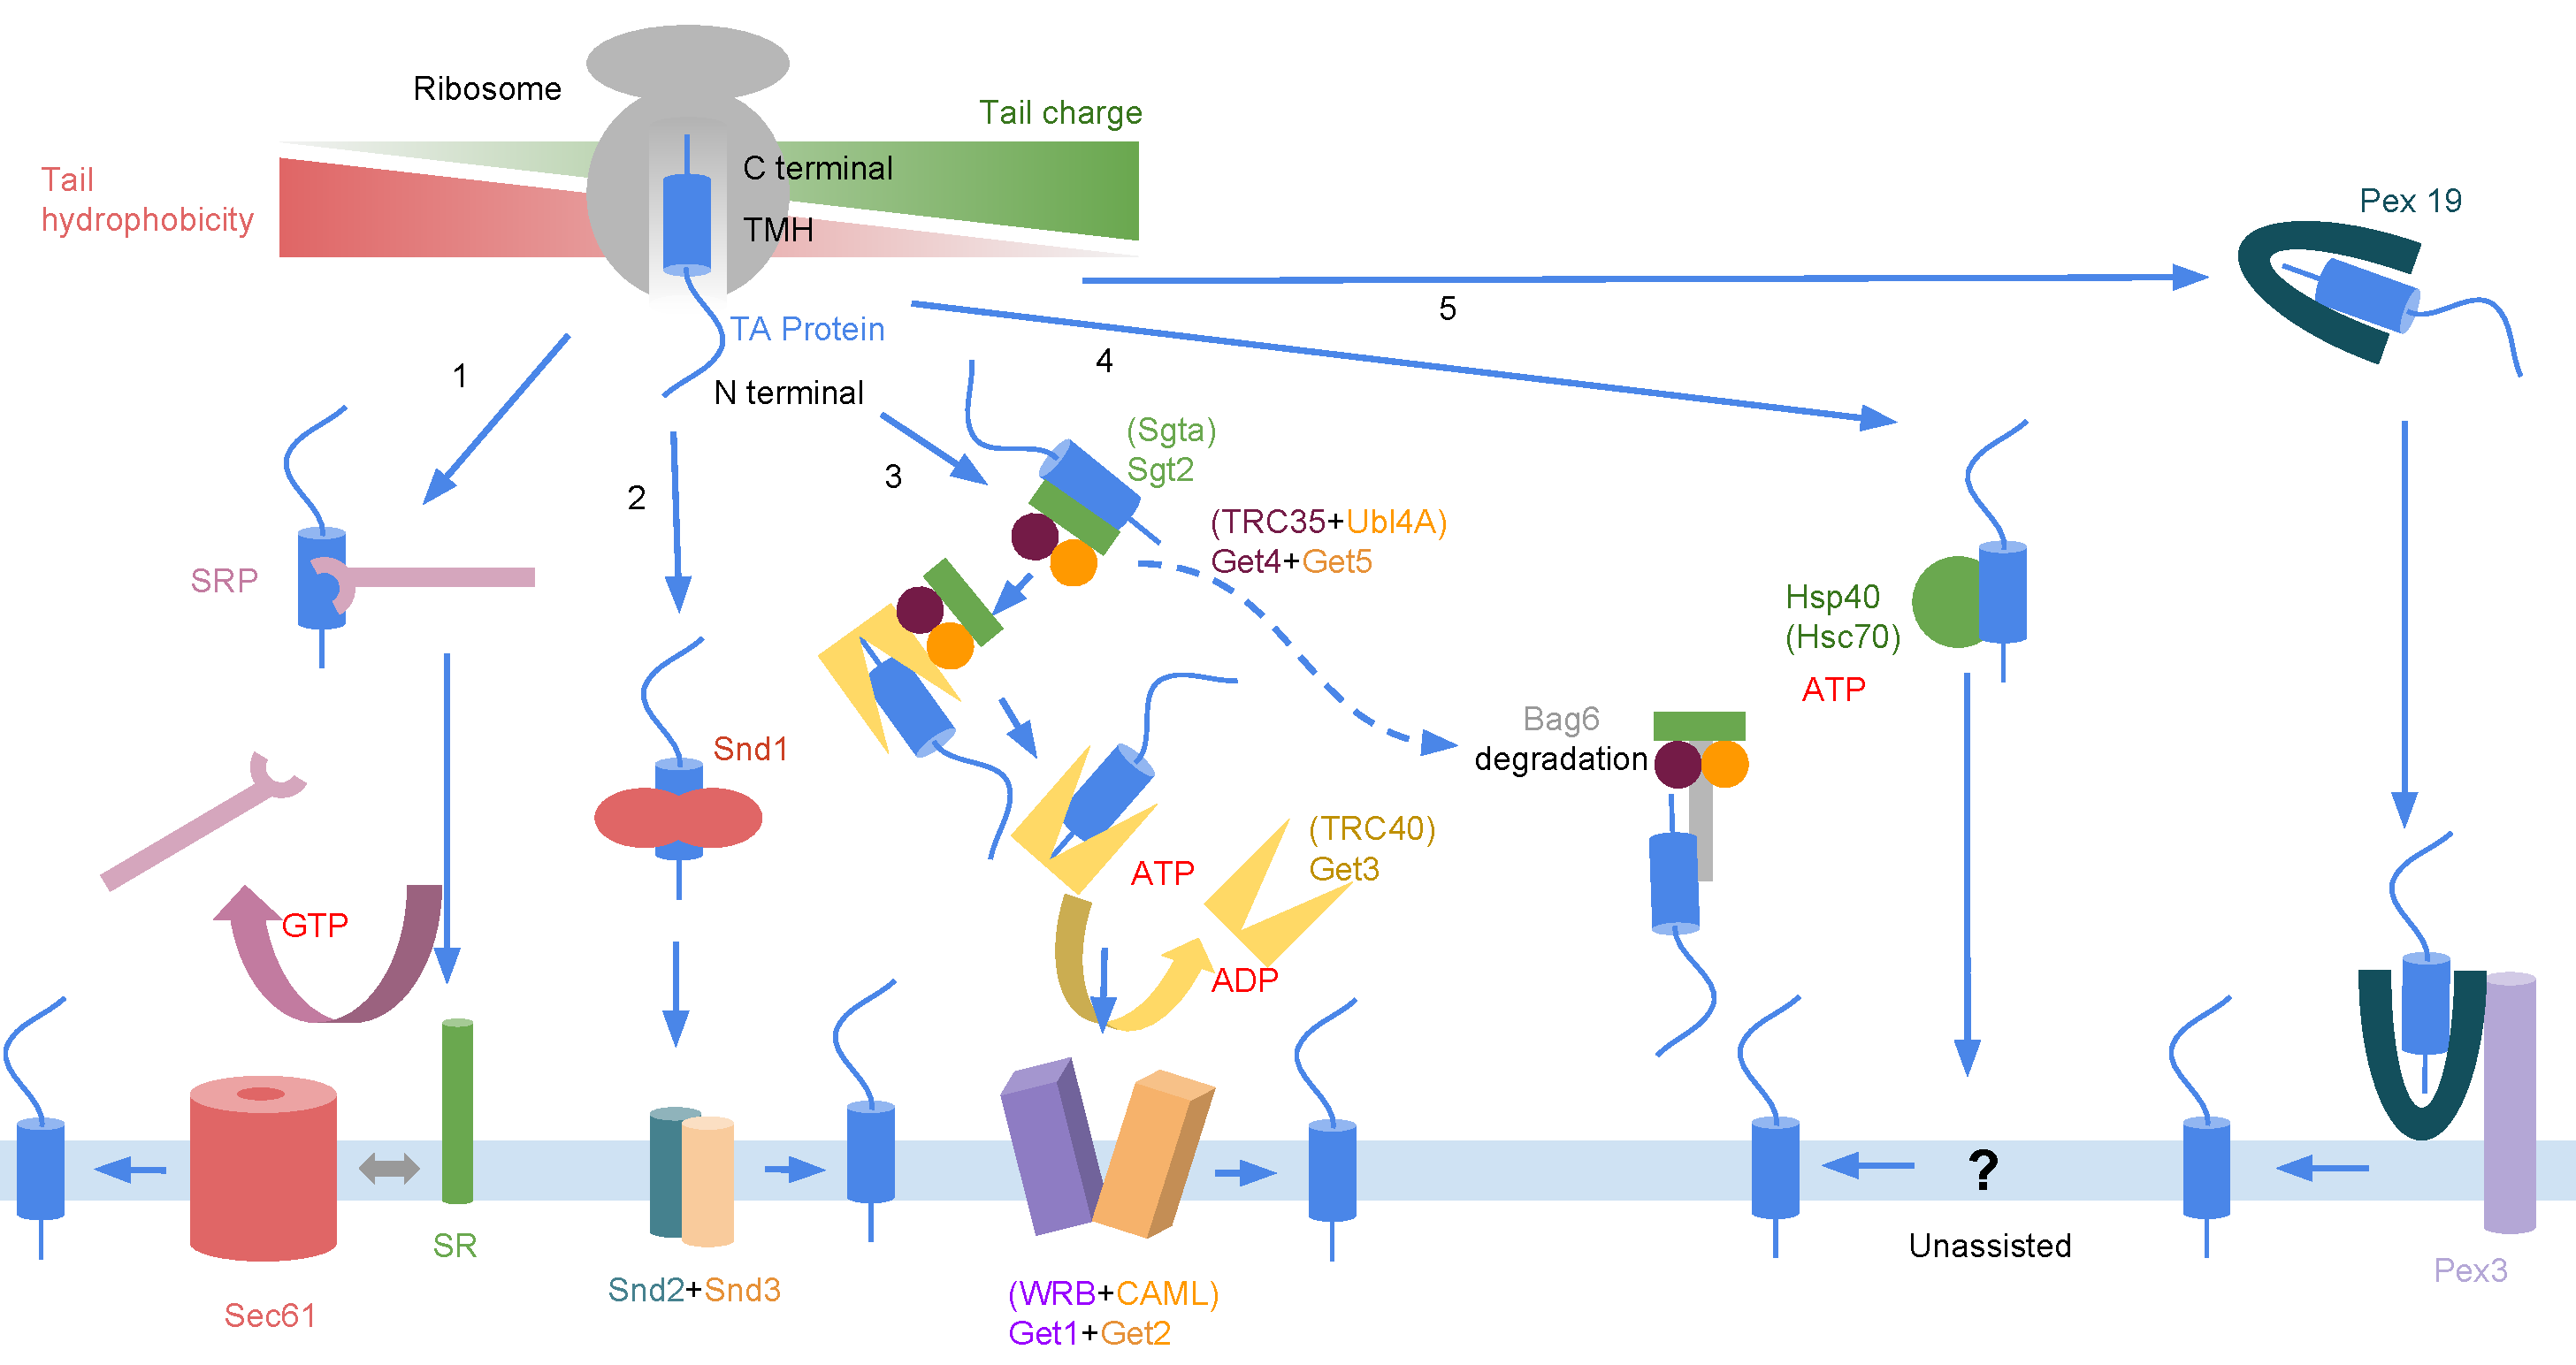
\includegraphics[width=1\textwidth]{TA_chapter/biogenesis-overview}
		\captionof{figure}[An overview of the biogenesis of tail anchored proteins.]{\textbf{An overview of the biogenesis of tail anchored proteins.}
		(1) \gls{srp} and Sec61 of the cotranslational insertion mechanism have been shown to be able to integrate \gls{ta} proteins.
		(2) In yeast a novel mechanism was identified in which Snd1 binds to the folded \gls{ta} protein and delivers it to the membrane bound Snd2 and Snd3 complex.
		(3) The intensively studied Get (yeast) or TRC40 (mammalian) pathway can target either for membrane integration or degradation of the \gls{ta} protein.
		(4) A handful of \gls{ta} proteins with relatively polar \gls{tmh} regions have been observed spontaneously integrating into the membrane using Hsp40 and Hsc70 as chaperones.
		Adapted from Johnson \textit{et al.,} 2013 and Guna \textit{et al.,} 2018.
}

\label{fig:biogenesis-overview}
\end{figure}

\gls{ta} proteins have several pathways for biogenesis in the~\gls{er} membrane.
These mechanisms include the Hsp40/Hsc70 chaperone system~\cite{Rabu2008}, the intensly studied TRC40/Get3 ATP dependent pathway ~\cite{Johnson2013, Chartron2012, Wang2014}, as well as some evidence supporting the use of the co-translational machinery.
\gls{ta} proteins were originally thought to be inserted into the membrane via different machinery than the co-translational machinery, but unexpectedly \gls{srp} was found to be a factor for post-translational targetting confirmed by both cross linking studies \cite{Abell2004} and an \textit{in vitro} pull down experiment \cite{Leznicki2010}.
\gls{srp} would deliver the \gls{ta} protein to the membrane bound \gls{sr} in association with a highly conserved Sec translocon.
Further cross-linking experiments suggested Sec61 is also involved during \gls{ta} protein membrane insertion \cite{Abell2003}.
Previous studies had shown the Sec61 translocon is not necessary for \gls{ta} protein membrane integration by biochemical reconstitution experiments \cite{Kutay1993} and conditional mutants in yeast \cite{Steel2002, Yabal2003}. %What kind of mutants?
This suggests the possibility of at least one insertion mechanism that is related to the co-translational method of insertion.

A second, possibly redundant, system is also known to be involved in \gls{ta} protein biogenesis and is referred to as the TRC40 (also known as Asna1) pathway in mammals.
A conserved homologue was found in \textit{Saccharomyces cerevisiae}, Get3 \cite{Schuldiner2008}, and in yeast this mechanism is generally referred to as the Get pathway.
Unlike the cotranslational machinery, the post-translational proteins do not couple with the ribosome, so the \gls{ta} protein must be exposed to the cytosolic environment for at least some time \cite{Guna2018}.
At some point after the \gls{ta} protein emerges from the ribosomal exit tunnel, the \gls{ta} protein \gls{tmh} associates with Sgt2.
An \textit{in vitro} assay revealed that Sgt2 associates with Get5  \cite{Wang2010} as part of a dimerised Get4 and Get5 complex (two copies of each)\cite{Chang2010, Chang2012, Chartron2010, Chartron2012}.
At this point Sgt2 either associates with preferential Get3 which targets the \gls{ta} protein for \gls{er} membrane biogenesis, or if there are excess \gls{ta} proteins Sgt2 also associates with Bag6 which targets the \gls{ta} protein for degradation \cite{Shao2017}.
This ``race'' between Bag6 and Get3 ensures a level of quality control within the system.
Assuming the \gls{ta} protein is not targetted for degradation, Get3 associates first with this complex via an interaction with the N-terminal of Get4 \cite{Wang2010}.
A dimerised ADP-bound Get3 \cite{Mateja2009, Hu2009, Bozkurt2009, Suloway2009, Yamagata2009} (TRC40) associates with and shields the C-terminal region of the \gls{ta} protein \cite{Stefanovic2007, Schuldiner2008, Favaloro2008}.
This shielding may be especially important since Get3 is involved in the folding of any nascent \gls{ta} proteins, which would be unviably hydrophobic in the cytosol \cite{Jonikas2009}.
Fluoresence studies revealed that tagged Get3 appears at both the cytosol and the \gls{er} membrane so apparently shuttles the \gls{ta} protein between the transmembrane complex of Get1 and Get 2 (WRB and CAML), that contains cytosolic domains that recieve Get3, and Get4 Get5 Sgt2 complex \cite{Huh2003, Zalisko2017}.
Yet it is an interesting note that a single molecule fluoresence study revealed that the minimum machinery required for \gls{ta} protein insertion from this system is a Get1 and Get2 heterodimer \cite{Zalisko2017}.

Redundancy of the Get/TRC40 pathway and \gls{srp} pathway may be explained in part by a novel \gls{srp} and Get independent pathway.
This pathway utilises the Snd protein pathway and was discovered in yeast \cite{Aviram2016}.
Snd1 binds to the \gls{ta} protein after it exits the ribsosome and delivers it to the Snd2 and Snd3 membrane bound complex which integrate the \gls{ta} protein into the membrane.

In the absence of the Get machinery, Hsp40 and Hsc70 chaperones along with ATP are also sufficient for enough biogenesis of \gls{ta} proteins for viable cell growth \cite{Rabu2008, Rabu2009, Ngosuwan2003, Colombo2009, Kemper2008, Meineke2008, Setoguchi2006}.
Chimeric synaptobrevin, one of the first identified~ \gls{snare} proteins, is capable of spontaneous insertion if the tail anchor domain is replaced by the~\gls{tm} domains belonging to a protein of known spontaneously inserting domains. %citation
Molecular dynamics simulations showed that direct insertion \gls{tmh}s thermodynamically mimics the energies of \gls{tmh}s integrated by the translocon \cite{Ulmschneider2014} so in theory no integration machinery is strictly necessary if the \gls{tmh} can ``correctly'' interact with the membrane interface.
Altering the hydrophobicity, at least in the case of the spontaneously inserting PTP1b, also determinates the localisation of the \gls{ta} protein to either the mitochondrial membrane or the \gls{er} membrane, or rather a more hydrophobic \gls{ta} protein \gls{tmh} is less likely to localise to the mitochondrial membrane \cite{Fueller2015}.
Further, it was revealed that scrambling the \gls{tmh} sequence, but maintaining hydrophobicity, reduced the insertion potential of spontaneously inserting \gls{tmh}s \cite{Brambillasca2006}.
This phenomenon cannot therefore be explained entirely by marginal hydrophobicity of the \gls{tmh}.

Given a ``choice'', it is speculated that hydrophobicity determines the integration pathway since Sec61$\beta$ has a hydrophobic \gls{tmh} and is targetted via the \gls{srp} pathway, whereas marginally hydrophobic \gls{ta} proteins like cytochrome b5 and PTP1b can spontaneously insert \textit{in vitro} and biologically only rely on Hsp70 and Hsc40.
Broader analysis has shown that hydrophobicity \cite{White1999} stratified by TM tendency score \cite{Zhao2009} can distinguish between the \gls{er} and mitochondrial localised \gls{ta} proteins \cite{Guna2018}.
However, the trememndous diversity and known biogenesis redundancy of these proteins may mean that no single factor applied en masse may be able to distinguish the \gls{tmh} recognition factors and investigation into this area is becoming increasingly complex \cite{Guna2018}.

By regenerating a list of likely \gls{tmh}s \cite{Kalbfleisch2007} and using a manually curated list of \gls{ta} proteins \cite{TheUniProtConsortium2014}, this investigation aims to find relationships between biochemical factors and a disposition to a certain insertion mechanism and terminal localisations.
Here, we also present evidence for a conserved polar strip along the spontaneously inserting \gls{ta} protein \gls{tmh}s, which may be the key to the initial interaction of these \gls{tmh}s with the membrane interface.



\section{Methods}

\subsection{Building a List of Tail-Anchors}
Steps carried out by Kalbfleisch \textit{et al.} published in Traffic 2007 (8: 1687\-1694)~\cite{Kalbfleisch2007}, were recreated using up to date tools.
Whilst their study focused on the human proteome, here we take into account the entire TrEMBL and SwissProt database and then stratify the datasets by the organism at the end of the pipeline (Figure \ref{fig:dataset-overview}).

\begin{figure}[!ht]
\centering
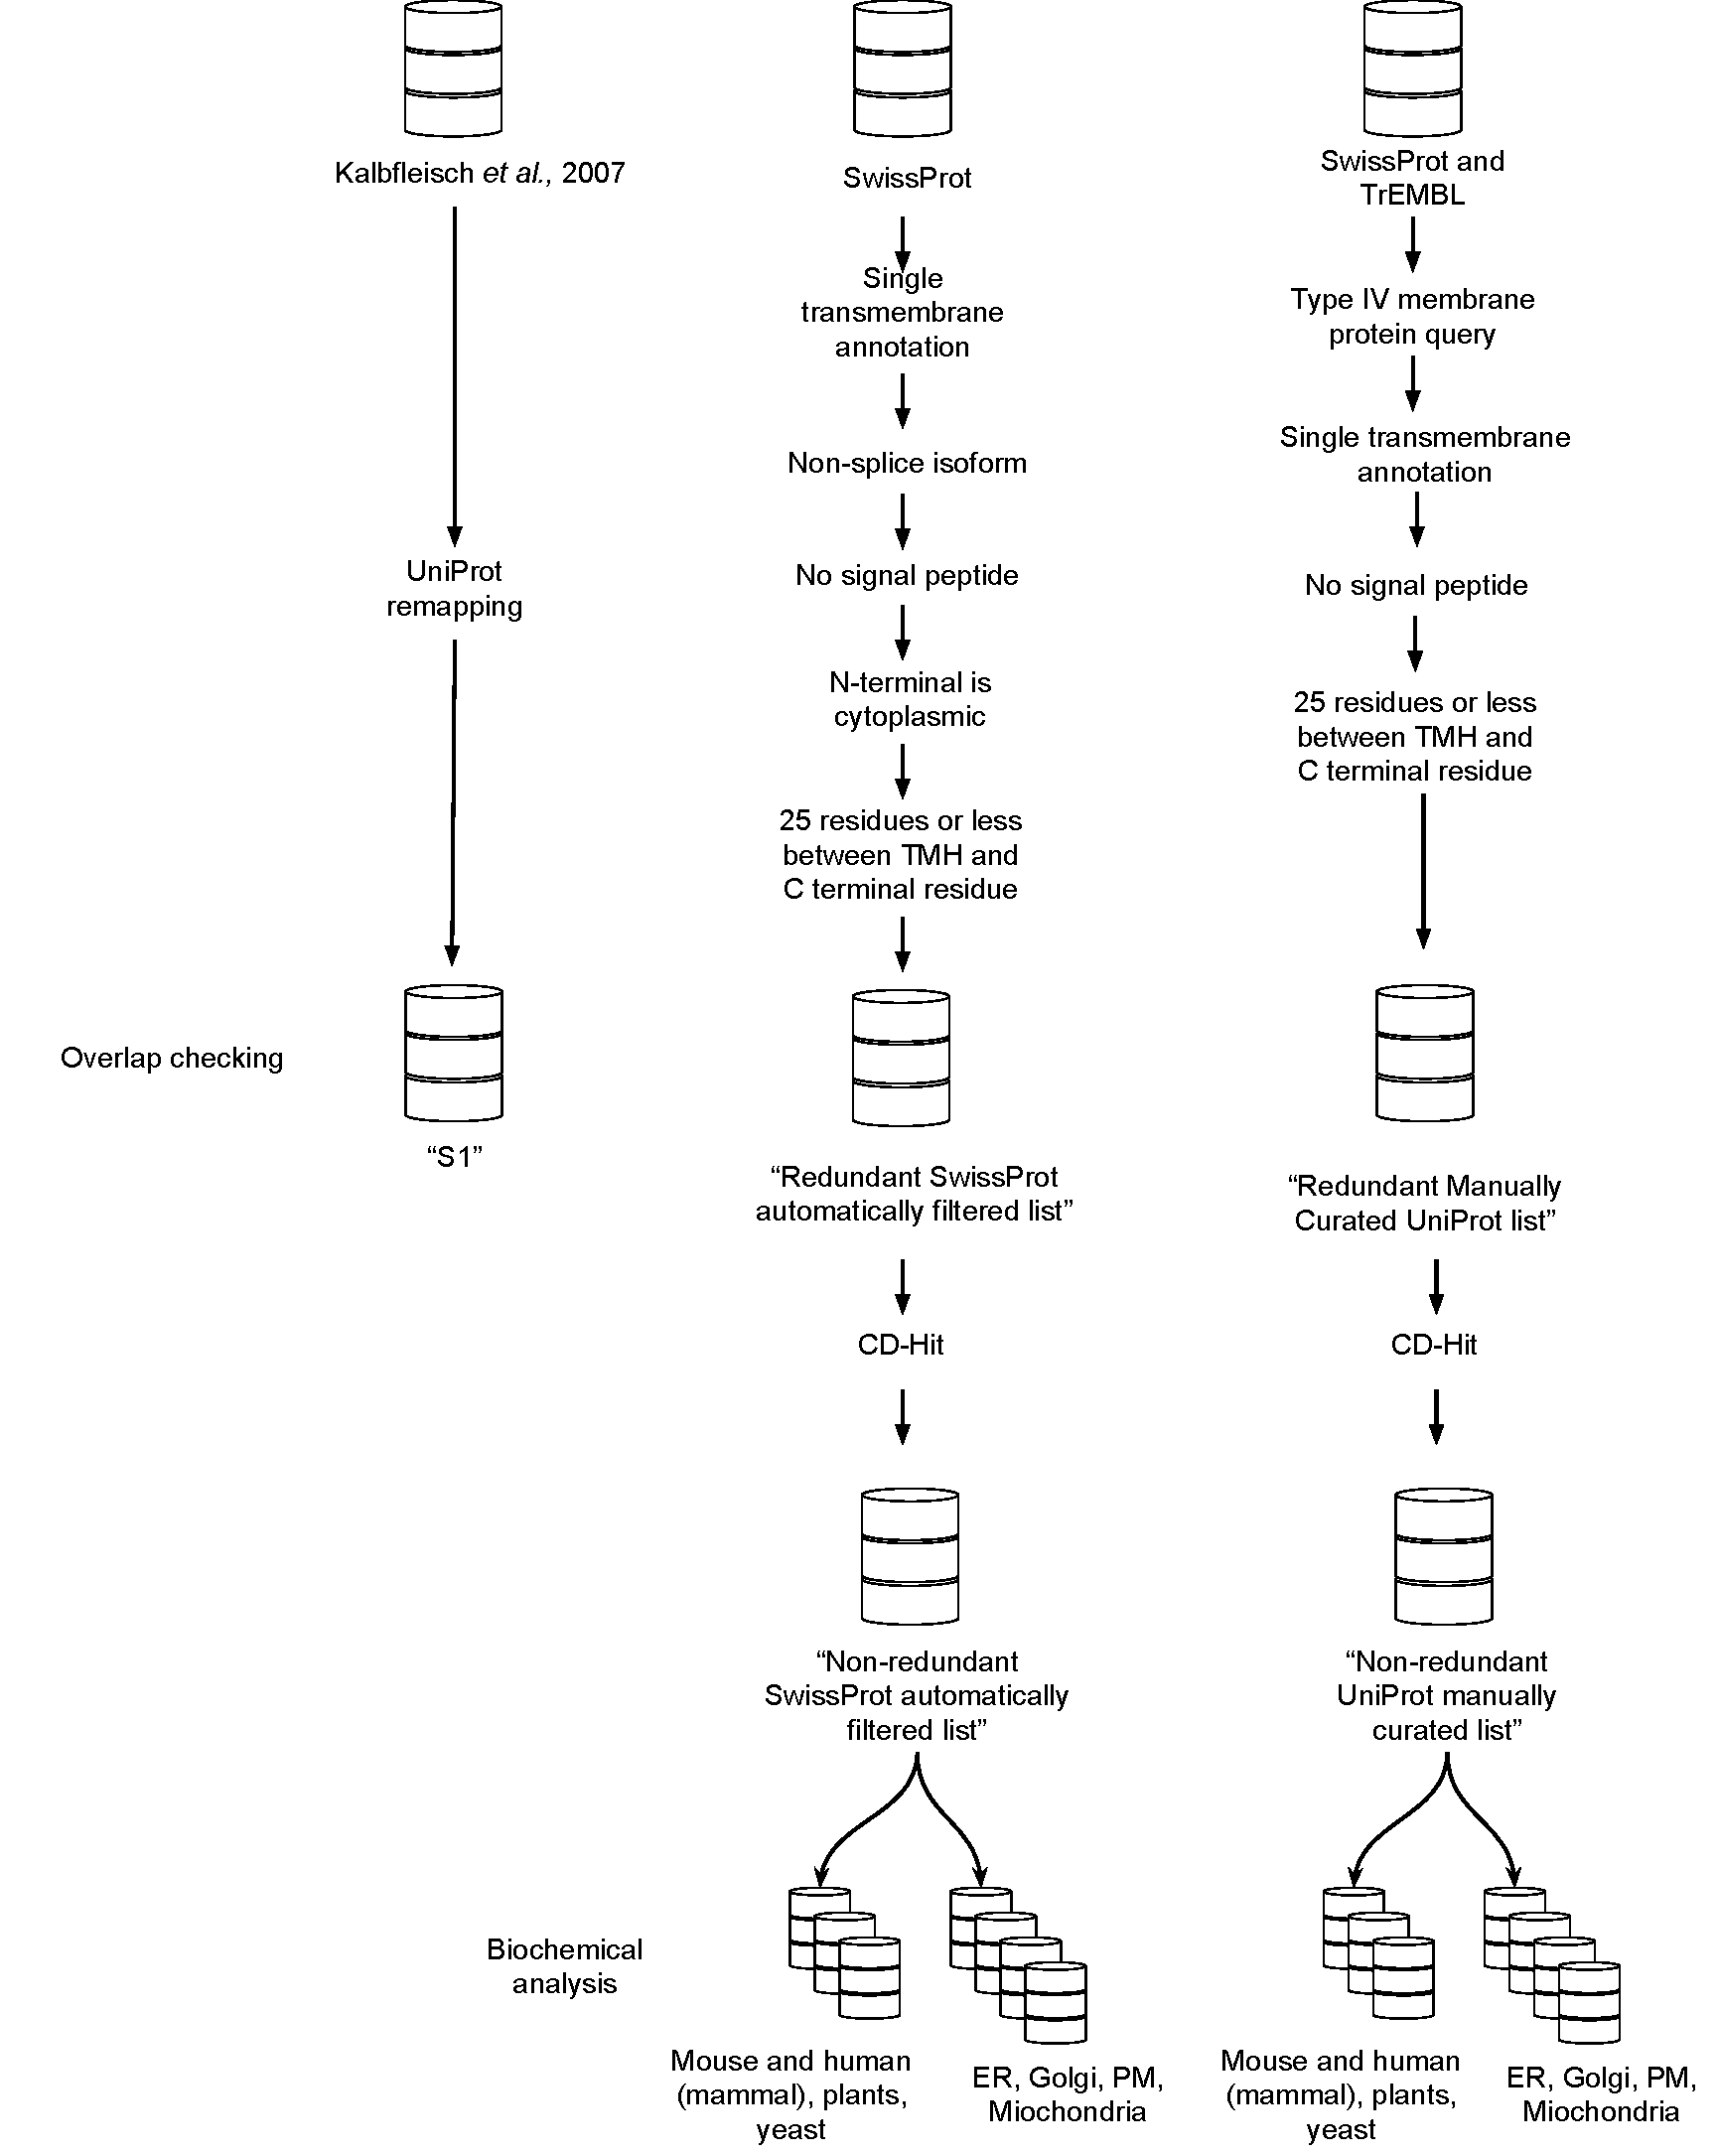
\includegraphics[width=1\textwidth]{TA_chapter/dataset-overview}
		\captionof{figure}[The sources, methods, and filters applied to the sequences in the datasets.]{\textbf{The sources, methods, and filters applied to the sequences in the datasets.}
		From top to bottom are the sources of the sequences and the filters and methods applied to each of the datasets of sequences. The database sybmol is used to denote when the dataset was used to capture results, and is available as supplementary material. For the dataset size and more information, see the methods section herein.
}

\label{fig:dataset-overview}
\end{figure}

\subsubsection{SwissProt Tail Anchored Dataset According to Filters}
There were 557012 protein records downloaded from SwissProt via UniProt~\cite{TheUniProtConsortium2014} (Downloaded 24--04--2018).
106149~\gls{tmh}s (\url{TRANSMEM} annotation) were found between 76953 records (\url{annotation:(type:transmem) AND reviewed:no}).
This keyword is contained in a record according to either experimental evidence~\cite{TheUniProtConsortium2014} or a robust meta-analysis of~\gls{tmh} prediction using TMHMM~\cite{Krogh2001}, Memsat~\cite{Jones2007}, Phobius~\cite{Kall2004,Kall2007} and the hydrophobic moment plot method of Eisenberg and co-workers~\cite{Eisenberg1984}.
11141 of those records had only a single~\gls{tmh}.
11110 of those~\gls{tmh}s were within the length thresholds of 16 to 30 residues (None of those had the annotation for splice isoforms according to \url{NON_TER} annotation).
5548 of those had had no~\gls{sp} annotation (\url{SIGNAL}).
4332 of those had annotation (based on \url{TOPO_DOM} annotation) that the N terminal was cytoplasmic.
615 of those had the~\gls{tmh} within 25 residues of the C terminal, the same threshold used by Kalbfleisch and their coworkers~\cite{Kalbfleisch2007}.
Running CD-Hit 4.5.3 on the WebMGA web-server~\cite{Huang2010, Wu2011} at 90\% identical sequence at 90\% coverage thresholds resulted in 443 representative proteins.
This threshold was chosen as a compromise between avoiding over-representation of a certain protein and maintaining a viable sample size.

From this representative list, 46 were Archaeal, 66 were bacterial, and 320 were Eukaryotic and 11 came from dsDNA viruses.
When counting proteomes with greater than 20 records, 49 belonged to the \textit{A. thaliana} proteome, 48 to Mouse, 46 to the human proteome, 24 to \textit{S.cerevisiae}. %19 from RAT!

65 were annotated under the Mitochondrion location (query \url{locations:(location:"Mitochondrion [SL-0173]")}), 157 in the \gls{pm} (query \url{locations:(location:"Cell membrane [SL-0039]")}, 82 in the Golgi (query \url{locations:(location:"Golgi apparatus [SL-0132]")}), and 98 in the \gls{er} (query \url{locations:(location:"Endoplasmic reticulum [SL-0095]"}).

\subsubsection{TrEMBL Tail Anchored Dataset According to Filters}
111425234 records were stored in the TrEMBL database at time of download (Downloaded 25--04--2018).
22107826 of those contained \url{TRANSMEM} annotation (\url{annotation:(type:transmem) AND reviewed:no}).
18053 of these were single-pass proteins.
All of these were within the length restrictions.
17973 of those did not contain a signal sequence when looking for \url{SIGNAL} annotation.
5157 of those contained a cytoplasmically located N terminal according to \url{TOPO_DOM} annotation.
155 records had a~\gls{tmh} within 15 residues of the C terminal residue.
In those record's annotations, no more than 1 appeared in any given species, so they were omitted from the SwissProt list sequence redundancy protocol to avoid representing a well-annotated record with a poorly annotated record.

\subsubsection{UniProt Curated List}
A query for \url{locations:(location:"Single-pass type IV membrane protein [SL-9908]")} was used in UniProt which returned 2633 UniProtKB IDs; 463 SwissProt results and 2170 TrEMBL results.
This manaully created list contained some \gls{ta} proteins that didn't fit the generally accepted definition of a \gls{ta} protein and were excluded from further analysis.
101 exceeded the \gls{ta} length restrictions of 25 residues between the \gls{tmh} and the terminal residue.
8 contained annotation for \url{SIGNAL}, indicating a \gls{sp}, inconsistent with the \gls{ta} protein definition.
20 were multipass proteins.
A full list of which records exceeded these limits and by how much is included in the supplementary files.
Running these records through CD-HIT at 90\% redundancy yielded 956 clusters; 269 SwissProt records and 687 TrEMBL records~\cite{Huang2010, Wu2011}.
No further filters were applied to this list.
Proteomes represented by more than 20 records include \textit{A. thaliana} (53 records), Humans (30), Mouse (30), and \textit{S. cerevisiae} (27). % and 20 to Rat.

426 were annotated under the Mitochondrion location (query \url{locations:(location:"Mitochondrion [SL-0173]")}) 47 from SwissProt and 379 automatically assigned in TrEMBL.
397 in the \gls{er} (query \url{locations:(location:"Endoplasmic reticulum [SL-0095]")}), 88 from SwissProt and 308 automatically annotated in TrEMBL.
1 TrEMBL record (A0A1E5RT24) in the \gls{er} set contained an ``X'' residue in the C terminal flank and was omitted from the analyses.
Two subcellular location datasets had no automatically ascribed records and only contained manually annotated SwissProt records; 31 in the \gls{pm} (query \url{locations:(location:"Cell membrane [SL-0039]")}, and 83 in the Golgi (query \url{locations:(location:"Golgi apparatus [SL-0132]")}).

\subsubsection{Remapping Previous Dataset}
189 of the 411 proteins from the previous study~\cite{Kalbfleisch2007} were successfully mapped to 222 UniProtKB IDs using the UniProt mapping tools with the RefSeq Protein to UniProtKB option~\cite{TheUniProtConsortium2014}.

\subsubsection{Tail Anchor Protein Chaperone Interactors}
BioGrid interactors for the chaperones were downloaded.

These interactor lists were filtered through the SwissProt automatically filtered and the UniProt curated \gls{ta} protein datasets.
There were 91 interaction pairs for Hsp40 which mapped to 206 UniProt records.
Hsc70 had 534 interaction pairs 61 of which were mapped to 91 UniProt records.
Hsp40 and Hsc70 both returned 0 record hits after filtering the UniProt records ids through the UniProt manually curated list and the automatically generated SwissProt list both before redundancy removal.

Snd1 had 237 interaction pairs which mapped to 239 records.
Snd1 returned 15 hits when filtering it through the \gls{ta} datasets.

SGT2 had 260 BioGrid interactor ids which mapped to 264 UniProt records.
SGTA had 155 interactor ids from BioGrid, 153 of which were mapped to 274 records.
SGT2 and SGTA returned 14 and 5 hits respectively.

50 BioGrid ids from TRC40 interaction pairs were mapped to 90 UniProt records.
Get3 had 456 Biogrid interactor ids, which mapped to 465 UniProt records.
After filtering those records throught the \gls{ta} anchor datasets TRC40 and Get3 returned 7 and 22 hits respectively.


\subsection{Calculating Hydrophobicity}
Windowed hydrophobicity was calculated using a window length of 5 residues, and half windows were permitted.
Average hydrophobicity takes the total of the raw amino acid hydrophobicity values and divides them by the number of amino acids in the slice.
Values reported in the results are based on the Kyte \& Doolittle scale~\cite{Kyte1982} which is based on the water\---vapour transfer free energy and the interior-exterior distribution of individual amino acids.
%Hydrophobicity values were also validated by the White and Wimley scale~\cite{White1999}, the Hessa scale~\cite{Hessa2005}, and the Eisenberg scale~\cite{Eisenberg1984}.

\subsection{Calculating Sequence Information Entropy}
Information entropy, is essentially an estimate of the linguistic entropy of a string.
In the context of biology, it can be thought of as an estimation of the non-randomness of a sequence.
Sequence complexity can be used to analyse DNA sequences~\cite{Pinho2013, Oliver1993, Troyanskaya2002}, and is a component of the TMSOC z-score which can predict function beyond anchorage of a \gls{tmh}~\cite{Wong2011, Wong2012, Baker2017}.
here we focus on the analysis of the complexity of a sequence in protein sequences.

Broadly speaking, the information theory entropy of a linguistic string can be defined as in equation~\ref{simpleentropy2}, and we treat the protein sequence \gls{tmh} as a string with or without its flanking regions.

\begin{equation} \label{simpleentropy2}
	H(S)=-{\sum_{i=1}^n {p_i\log_s(p_i)}}
\end{equation}

Where H is the entropy of a sequence (S), and $p_i$ is the probability of a character $i$ through each position (n) in S. This allows us to quantify the average relative information density held within a string of information~\cite{Shannon1948}.

\subsection{Statistics}

The null hypothesis of homogeneity of two distributions was examined with the Kolmogorov Smirnov, the Kruskal-Wallis, and the 2-sampled Student's T-test statistical tests.
These tests were all ran through the Python SciPy stat package v0.17 python package~\cite{VanderWalt2011}.
To note, the~\gls{ks} test scrutinises for significant maximal absolute differences between distribution curves; the~\gls{kw} test is after skews between distributions and the student t-test statistical test checks the average difference between distributions.

Since the P‑value is a product of a fraction of test statistics obtained from a permutated set of the samples, it exponentially increases as N increases; the P-value is a strong function of N.
We rely on the Bahadur slope ($B$) as a measure of distance between two distributions~\cite{Bahadur1967, Bahadur1971, Sunyaev1998, Baker2017}. A larger Bahadur slope shows a greater difference between the two distributions.

\begin{equation} \label{eq:bahadur2}
B=\frac{|\ln(P~value)|}{N}
\end{equation}

\subsection{Modelling Cytochrome b5 and PTP1b}
The HHpred webserver was used to query homologues of and model templates for Cytochrome b5 (UniProt accession code P00167) and PTP1b (UniProt accession code P18031)~\cite{Soding 2005, Soding 2005a}.
Homologues were queried using three iterations of HHblitscd against the sequence database version uniprot20\_2016\_02 to generate the query Hidden Markov Model.
The choice of templates was driven by the quality and coverage of the alignments and of the quality of the models that resulted.
For cytochrome b5, a multiple alignment was generated from PDB accession codes 2M33, 2KEO, 3X34, 1MJ4, 1MJ4, 2IBJ covering the globular domain, and PDB accession codes 5NAO, 5DOQ, 5NAM, and 2MMU covering the \gls{tmh}.
Modeller was ran from within the HHPRED server to generate the homology model \cite{Eswar2007,Zimmerman2017,Webb2016}.
The model was confirmed to be of high quality using ProSA (Z-Score: -4.61) \cite{Wiederstein2007}, Ramachandran plot on the RAMPAGE webserver (98\% allowed residues, including all \gls{tmh} residues) \cite{Lovell2003}.

The coverage and alignment quality of PTP 1b was however, not as good quality.
Although UniProt holds 145 associated PDB structures for PTP1b, these structures cover at least some part of the globular domains of the protein.
There are no PDB structures for the \gls{tm} domain or the nearby flanking regions.
Instead of a global protein model only the \gls{tmd} was modelled using a homology model derived from a single sequence alignment of 5NAO based on the TMH$\pm$6 residues of PTP1b.
%Verify3D \cite{Luthy1992}, and PROCHECK \cite{Laskowski1993}.

%>P1;UKNP
%sequence:UKNP:1    :A:137  :A::::
%MAEQSDEAVKYYTLEEIQKHNHSK-STWLILHHKVYDLTKFLEEHPGGEEVLREQAGGDATE--NFEDVGHSTDAREMSKTFIIGELHPDDRPKLNKPPETLITTIDSSSSWWTNWVIPAISAVAVALMYRLYMAED*
%>P1;2M33
%structure:2M33:1   :A:104 :A::Oryctolagus cuniculus::
%MAAQSDKDVKYYTLEEIKKHNHSK-STWLILHHKVYDLTKFLEEHPGGEEVLREQAGGDATE--NFEDVGHSTDARELSKTFIIGELHPDDRSKLSKPMETLITTVD------------------------------*
%>P1;2KEO
%structure:2KEO:21  :A:112 :A::Homo sapiens::
%------EKVTLVRIADLENHNNDG-GFWTVIDGKVYDIKDFQTQSLTENSILAQFAGEDPVV--ALEAALQFEDTRESMHAFCVGQYLEPDQEGVTIPDLG------------------------------------*
%>P1;3X34
%structure:3X34:8   :A:92  :A::Sus scrofa:0.76:
%-------AVKYYTLEEIQKHNNSK-STWLILHHKVYDLTKFLEEHPGGEEVLREQAGGDATE--NFEDVGHSTDARELSKTFIIGELHPDDRSKI------------------------------------------*
%>P1;1MJ4
%structure:1MJ4:3   :A:82  :A::Homo sapiens:1.2:
%-------STHIYTKEEVSSHTSPETGIWVTLGSEVFDVTEFVDLHPGGPSKLMLAAGGPLEPFWALYAVHNQSHVRELLAQYKIGEL--------------------------------------------------*
%>P1;2IBJ
%structure:2IBJ:3   :A:88  :A::Musca domestica:1.55:
%-----SEDVKYFTRAEVAKNNTKD-KNWFIIHNNVYDVTAFLNEHPGGEEVLIEQAGKDATE--HFEDVGHSSDAREMMKQYKVGELVAEERSN-------------------------------------------*
%>P1;5NAO
%structure:5NAO:16  :A:34  :A::Homo sapiens::
%-------------------------------------------------------------------------------------------------------------------VLSVLVVSVVAVLVYKFYF---*
%>P1;5DOQ
%structure:5DOQ:6   :C:28  :C::Geobacillus thermodenitrificans (strain NG80-2):3.05:
%------------------------------------------------------------------------------------------------------------------IMYAPMVVVALSVVAAFWVGLKD*
%>P1;5NAM
%structure:5NAM:16  :A:34  :A::Homo sapiens::
%-------------------------------------------------------------------------------------------------------------------VLSVLVVSVVAVLVYKFYF---*
%>P1;2MMU
%structure:2MMU:30  :A:53  :A::Mycobacterium tuberculosis::
%-------------------------------------------------------------------------------------------------------------SVWFVSLFIGLMLIGLIWLMVFQL----*

APBS as a PyMol plugin was used to map the electrostatic surface of the model \cite{Baker2001}.
Consurf \cite{Ashkenazy2010} was used to map the conservation scores based on 5 iterations of PSI-BLAST \cite{Altschul1997} with an E-value cut-off of 0.0001.
In the case of PTP 1b a sequence alignment was generated for the full sequence and mapped onto the \gls{tmd} structure.
Hydrophobicity was mapped according to the Eisenberg aggregated hydrophicity scale \cite{Eisenberg1984} using a script accessed at \url{https://pymolwiki.org/index.php/Color_h}.


\section{Results}

\subsection{A Comparison Of Up-To-Date Tail-Anchored Protein Datasets}
Here, we use two sources for \gls{ta} protein datasets.
One dataset is based on a previous method~\cite{Kalbfleisch2007} to obtain \gls{ta} datasets and consists of 9296 \gls{tmh} residues (13279 including up to $\pm$5 flanking residues) from 443 SwissProt entries with 90\% redundancy removal.
Another dataset contains the UniProt curated set of Type IV membrane proteins again with 90\% redundancy removal.
This dataset contains 20528 \gls{tmh} residues (27950 including up to $\pm$5 flanking residues) from 956 UniProt protein records.

% Venn diagram
\begin{figure}[!ht]
\centering
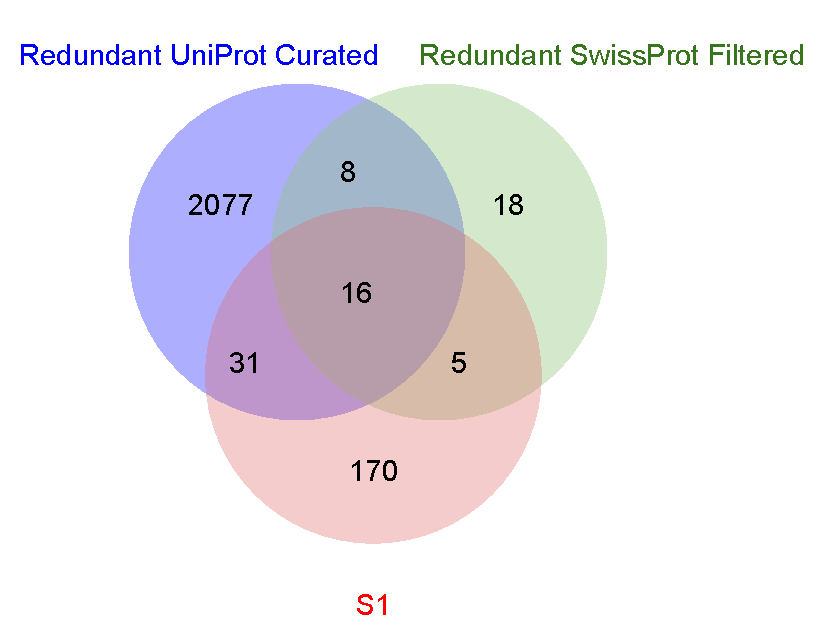
\includegraphics[width=0.5\textwidth]{TA_chapter/database-overlap}
		\captionof{figure}[A Venn diagram showing tail anchored protein UniProt ids present in each of the datasets as well as those present in multiple datasets.]{\textbf{A Venn diagram showing tail anchored protein UniProt ids present in each of the datasets as well as those present in multiple datasets.}
The number of ids present in redundant versions of
i) the supplementary materials table of a previous study predicting the complete set of human tail anchored proteins denote by S1~\cite{Kalbfleisch2007},
ii) the SwissProt dataset filtered according to typical~\gls{ta} features limited to the human proteome~\cite{TheUniProtConsortium2014}, and
iii) The UniProt curated list of~\gls{ta} proteins~\cite{TheUniProtConsortium2014}.
Note that to avoid losing IDs to redundancy reduction this diagram was generated without the use of CD-HIT~\cite{Huang2010, Wu2011}, which is applied in later statistical analysis.}

\label{fig:tadatasetoverlap}
\end{figure}

In order to get an understanding of the consistency of the datasets, before removing redundant proteins, we compared these two datasets to a dataset remapped set of proteins from a previous 2007 method~\cite{Kalbfleisch2007}.
The S1 dataset was built with an aim to gather \gls{ta} proteins in the human genome from the NCBI.
Note that these numbers are not absolutely certain.
The greatest source of uncertainty here is that the original S1 list includes 411 records, however only 222 of these were successfully mapped to the UniProt dataset.
This figure is closer to the 202 proteins from the original S1 list that excluded proteins that were either hypothetical or splice isoforms.
That being said, this mapping step prevents us from directly comparing the entire original S1 dataset.
We compared the up-to-date datasets to S1 to see how many records are shared, how many are now obsolete, and how many are unique.

Figure~\ref{fig:tadatasetoverlap} shows that S1 has 175 record ids of 222 records (78.8\%) which do not share overlap the up-to-date manually curated UniProt dataset~\cite{TheUniProtConsortium2014}.
Of the 170 unique records of that S1 dataset, 4 were manually annotated as not belonging to human, 20 have the C terminal as annotated being cytoplasmic, only 125 had \texttt{TRANSMEM} annotation indicating a bone fide \gls{tmh}.
If we apply equivalent filters, only 42 have annotation verifying that they are \gls{ta} proteins.

Equivalent criteria were applied to the entire SwissProt database and then restricted to the human proteome dataset.
24 of these 47 records (51.1\%) are in the curated UniProt~\gls{ta}  dataset.
21 of the 49 (44.7\%) records from SwissProt filtered human dataset can be found in the original S1 list.

The same method applied to an up-to-date dataset overlaps more with a manually curated dataset.
There is also a large degree of what we now believe to be mistakes that occurred in the older prediction tools and datasets, even when using similar methods.
As a trend, this shows that up-to-date datasets improve the reliability of this automated predicted method.
These automated criteria still do not fully align with the manually curated list.
Of 2633 records, only 2241 have the \texttt{TRANSMEM} annotation.
Ultimately, this points to the idea that datasets are a moving target as they are constantly updated with more accurate information using evermore reliable tools and methods.

\subsection{It Is Difficult To Observe Any Hydrophobic Variation Of TA Protein TMHs From Different Species}

In single-pass proteins of eukaryotic species there are typically various adaptations of the \gls{tmh} to adhere to the membrane constraints of the specific membrane.
For single-pass proteins, previous studies have observed differences in terms of \gls{tmh} hydrophobicity between yeast and human \gls{tmp}s~\cite{Sharpe2010}, or in cress, yeast, bacteria, and human datasets~\cite{Baker2017}.
We would expect to see a similar trend between the \gls{tmh}s of \gls{ta} proteins from different species.
However, when assuming a zero-difference hypothesis, in these \gls{tmh} \gls{ta} protein datasets we cannot observe any species-level differences between the datasets at this sample size for \gls{tmh} hydrophobicity.

% Average lines for figure, table for stats
When comparing the average Kyte \& Doolittle~\cite{Kyte1982} hydrophobicity values for the~\gls{tmh}s from humans and mice, \textit{A. thaliana}, and  \textit{S. cerevisiae}, we can see little difference between the mean values.
All of the mean values lie between 2.3-2.6 when we only consider the \gls{tmh} and at 1.3-1.6 when considering residues in close proximity to the~\gls{tmh} ($\pm$5 residues) (Figure~\ref{fig:average_species_hydrophobicity_ta}).

\begin{figure}[!ht]
\centering
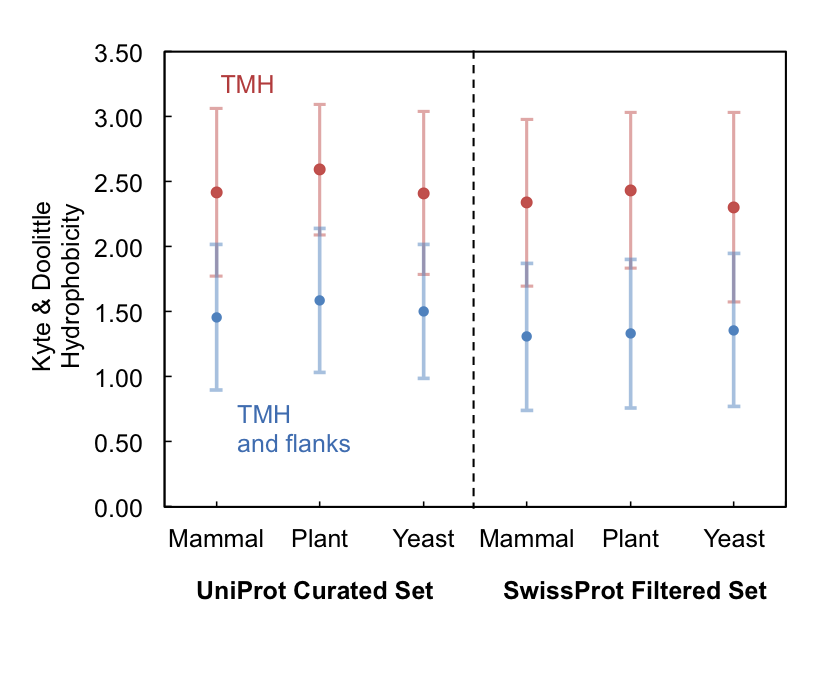
\includegraphics[width=1\textwidth]{TA_chapter/species-hydrophobicity}
\captionof{figure}[Average values of species datasets from UniProt manually curated set and SwissProt automatically filtered dataset.]
{\textbf{Average values of species datasets from UniProt manually curated set and SwissProt automatically filtered dataset.}

The average hydrophobicity values from the Kyte \& Doolittle scale~\cite{Kyte1982}.for both the \gls{tmh} and the \gls{tmh}$\pm$5 residues.
%and the GlobProt scale~\cite{Linding2003}
Values are shown for both the UniProt manually curated set and the SwissProt filtered set. In the UniProt manually curated set we compare the mammalian set of \gls{ta} proteins (Human N=30 and Mouse N=30) to \textit{A. thaliana} (N=57) representing plants and \textit{S. cerevisiae} (N=27) representing yeasts. For the SwissProt filtered set we compare the mammalian set of \gls{ta} proteins (Human N=46 and Mouse N=48) to \textit{A. thaliana} (N=49) representing plants  and  \textit{S. cerevisiae} (N=24) representing yeasts.
Error bars are shown at $\pm 1 \sigma$ from the mean of the respective dataset.
}

\label{fig:average_species_hydrophobicity_ta}
\end{figure}

Indeed, we see no strong observable statistical differences in hydrophobicity ($P>3.35E-1$ in the SwissProt automatically filtered list Table \ref{table:speciestableswissprotstats}, and $P>2.40E-1$ in the UniProt curated list Table \ref{table:speciestableuniprotstats}).
There are also no consistent trends among the absolute Bahadur slopes; no datasets are greatly different from any other.

\begin{table}[htbp]
\centering
\captionof{table}[Hydrophobicity statistical comparisons between mouse and human, yeast, and plants in the SwissProt Filtered Dataset.]
{\textbf{Hydrophobicity statistical comparisons between mouse and human, yeast, and plants in the SwissProt Filtered Dataset.}
Here, we compare a mammalian set of \gls{ta} proteins (Human N=46 and Mouse N=48) to \textit{A. thaliana} (N=49) representing plants  and  \textit{S. cerevisiae} (N=24) representing yeasts.
The hydrophobicity was predicted as the mean average of the values of the sequences of the \gls{tmh}, as well another group including up to $\pm$5 flanking residues, since predicting the boundary of \gls{tmh}s is difficult, according to the Kyte \& Doolittle hydrophobicity scale~\cite{Kyte1982}.
% Disorder was calculated in the same way using the GlobProt scale \cite{Linding2003}.
The Test column refers to the statistical score obtained from the test; H statistic for the Kruskal Wallis, the KS statistic for the Kolmogorov Smirnov test, and the t-statistic for the T-test.
$P$ is the P-value of that statistical score.
$B$ refers to the Bahadur slope, an interpretation of the P-value that accounts for the sample size powering the test~\cite{Bahadur1967, Bahadur1971}.}
\tiny
	% Table generated by Excel2LaTeX from sheet 'SwissProt filtered species'

    \begin{tabular}{clrrrrrrrrr}
          &       & \multicolumn{3}{c}{Mammal and Plant} & \multicolumn{3}{c}{Mammal and Yeast} & \multicolumn{3}{c}{Plant and Yeast} \\
          &       & \multicolumn{1}{l}{Test} & \multicolumn{1}{l}{$P$} & \multicolumn{1}{l}{$B$} & \multicolumn{1}{l}{Test} & \multicolumn{1}{l}{$P$} & \multicolumn{1}{l}{$B$} & \multicolumn{1}{l}{Test} & \multicolumn{1}{l}{$P$} & \multicolumn{1}{l}{$B$} \\
    \multirow{3}[0]{*}{TMH } &  Kruskal-Wallis & 0.93  & 3.35E-1 & 7.64E-3 & 0.10  & 7.56E-1 & 2.37E-3 & 0.84  & 3.60E-1 & 1.40E-2 \\
          &  Kolmogorov-Smirnov & 0.13  & 6.36E-1 & 3.17E-3 & 0.12  & 9.24E-1 & 6.69E-4 & 0.19  & 5.28E-1 & 8.76E-3 \\
          &  Student's T-test & -0.86 & 3.90E-1 & 6.58E-3 & 0.21  & 8.31E-1 & 1.57E-3 & 0.79  & 4.33E-1 & 1.15E-2 \\
    \multirow{3}[0]{*}{TMH and flanks } &  Kruskal-Wallis & 0.04  & 8.52E-1 & 1.12E-3 & 0.12  & 7.28E-1 & 2.69E-3 & 0.04  & 8.33E-1 & 2.51E-3 \\
          &  Kolmogorov-Smirnov & 0.11  & 7.72E-1 & 1.81E-3 & 0.13  & 8.79E-1 & 1.09E-3 & 0.11  & 9.80E-1 & 2.81E-4 \\
          &  Student's T-test & -0.22 & 8.23E-1 & 1.37E-3 & -0.38 & 7.04E-1 & 2.97E-3 & -0.19 & 8.50E-1 & 2.22E-3 \\
    \end{tabular}%
				\label{table:speciestableswissprotstats}

\end{table}%

\begin{table}[htbp]
\centering
\captionof{table}[Hydrophobicity statistical comparisons between mouse and human, yeast, and plants in the UniProt Curated Dataset.]
{\textbf{Hydrophobicity statistical comparisons between mouse and human, yeast, and plants in the UniProt Curated Dataset.}
Here, we compare a mammalian set of \gls{ta} proteins (Human N=30 and Mouse N=30) to \textit{A. thaliana} (N=53) representing plants  and  \textit{S. cerevisiae} (N=27) representing yeasts.
The hydrophobicity was predicted as the mean average of the values of the sequences of the \gls{tmh}, as well another group including up to $\pm$5 flanking residues, since predicting the boundary of \gls{tmh}s is difficult, according to the Kyte \& Doolittle hydrophobicity scale~\cite{Kyte1982}.
%Disorder was calculated in the same way using the GlobProt scale \cite{Linding2003}.
The Test column refers to the statistical score obtained from the test; H statistic for the Kruskal Wallis, the KS statistic for the Kolmogorov Smirnov test, and the t-statistic for the T-test.
$P$ is the P-value of that statistical score.
$B$ refers to the Bahadur slope, an interpretation of the P-value that accounts for the sample size powering the test~\cite{Bahadur1967, Bahadur1971}.}
	\tiny
	% Table generated by Excel2LaTeX from sheet 'SwissProt filtered species'

	\begin{tabular}{clrrrrrrrrr}
				&       & \multicolumn{3}{c}{Mammal and Plant} & \multicolumn{3}{c}{Mammal and Yeast} & \multicolumn{3}{c}{Plant and Yeast} \\
				&       & \multicolumn{1}{l}{Test} & \multicolumn{1}{l}{P} & \multicolumn{1}{l}{B} & \multicolumn{1}{l}{Test} & \multicolumn{1}{l}{P} & \multicolumn{1}{l}{B} & \multicolumn{1}{l}{Test} & \multicolumn{1}{l}{P} & \multicolumn{1}{l}{B} \\
	\multirow{3}[0]{*}{TMH} &  Kruskal-Wallis & 0.71  & 4.01E-01 & 8.09E-03 & 0.03  & 8.72E-01 & 1.57E-03 & 0.57  & 4.48E-01 & 1.00E-02 \\
				&  Kolmogorov-Smirnov & 0.13  & 6.93E-01 & 3.24E-03 & 0.13  & 9.11E-01 & 1.08E-03 & 0.20  & 4.16E-01 & 1.10E-02 \\
				&  Student's T-test & -0.93 & 3.55E-01 & 9.15E-03 & -0.11 & 9.13E-01 & 1.04E-03 & 0.64  & 5.22E-01 & 8.12E-03 \\
	\multirow{3}[0]{*}{TMH and flanks} &  Kruskal-Wallis & 1.37  & 2.42E-01 & 1.26E-02 & 0.38  & 5.36E-01 & 7.17E-03 & 0.08  & 7.80E-01 & 3.11E-03 \\
				&  Kolmogorov-Smirnov & 0.19  & 2.40E-01 & 1.26E-02 & 0.14  & 8.13E-01 & 2.38E-03 & 0.09  & 9.97E-01 & 3.21E-05 \\
				&  Student's T-test & -1.17 & 2.45E-01 & 1.24E-02 & -0.79 & 4.35E-01 & 9.58E-03 & 0.20  & 8.43E-01 & 2.14E-03 \\
	\end{tabular}%
					\label{table:speciestableuniprotstats}
	\end{table}%

Here, we are dealing with datasets at least an order of magnitude smaller than those broad studies \cite{Sharpe2010, Baker2017} which could explain the absence of the effect.
However this only goes to show that if there is an effect in \gls{ta} proteins, it is indeed weak between species.


\subsection{There Are Biochemical Differences Between Tail-Anchored TMHs From Different Organelles}
% Average lines for figure, table for stats

As in the case of species, \gls{tmh}s with different subcellular localisations on average  have different hydrophobicity.
This could be in part due to the variation in membrane potential across the different organelles~\cite{Qin2011, Worley1994, Schapiro2000}, the known lipid asymetry caused by sphingomyelin and glycosphingolipids on the non-cytosolic leaflet and phosphatidylserine and phosphatidylethanolamine in the cytosolic leaflet in the Golgi and \gls{pm} and lack of asymetry in the \gls{er}~\cite{Daleke2007, Devaux2004}.
Sphingomyelin is not present in the \gls{er} but is present in the Golgi~\cite{Futerman2005} and \gls{pm}~\cite{Li2007, Tafesse2007}.
Furthermore the \gls{pm} contains densly packed sphingolipids and sterols~\cite{Paolo2006}.
%Need a sentence on the mitochondrial membrane

%Need mitochondria reference, and numbers for the UniER etc.
These hydrophobic differences have already been observed in the mitochondria localised \gls{ta} protein \gls{tmh}.
Here we consider the \gls{ta} proteins at certain locations within the cell ignoring species, and we see clear differences in the biochemistry of the \gls{tmh}.
In the UniProt manually curated dataset, the Kyte \& Doolittle hydrophobicity scores rage from 1.7 in mitochondria to 2.7 in the \gls{pm} (Figure \ref{fig:average_organelle_factors_ta}A).

\begin{figure}[!ht]
\centering
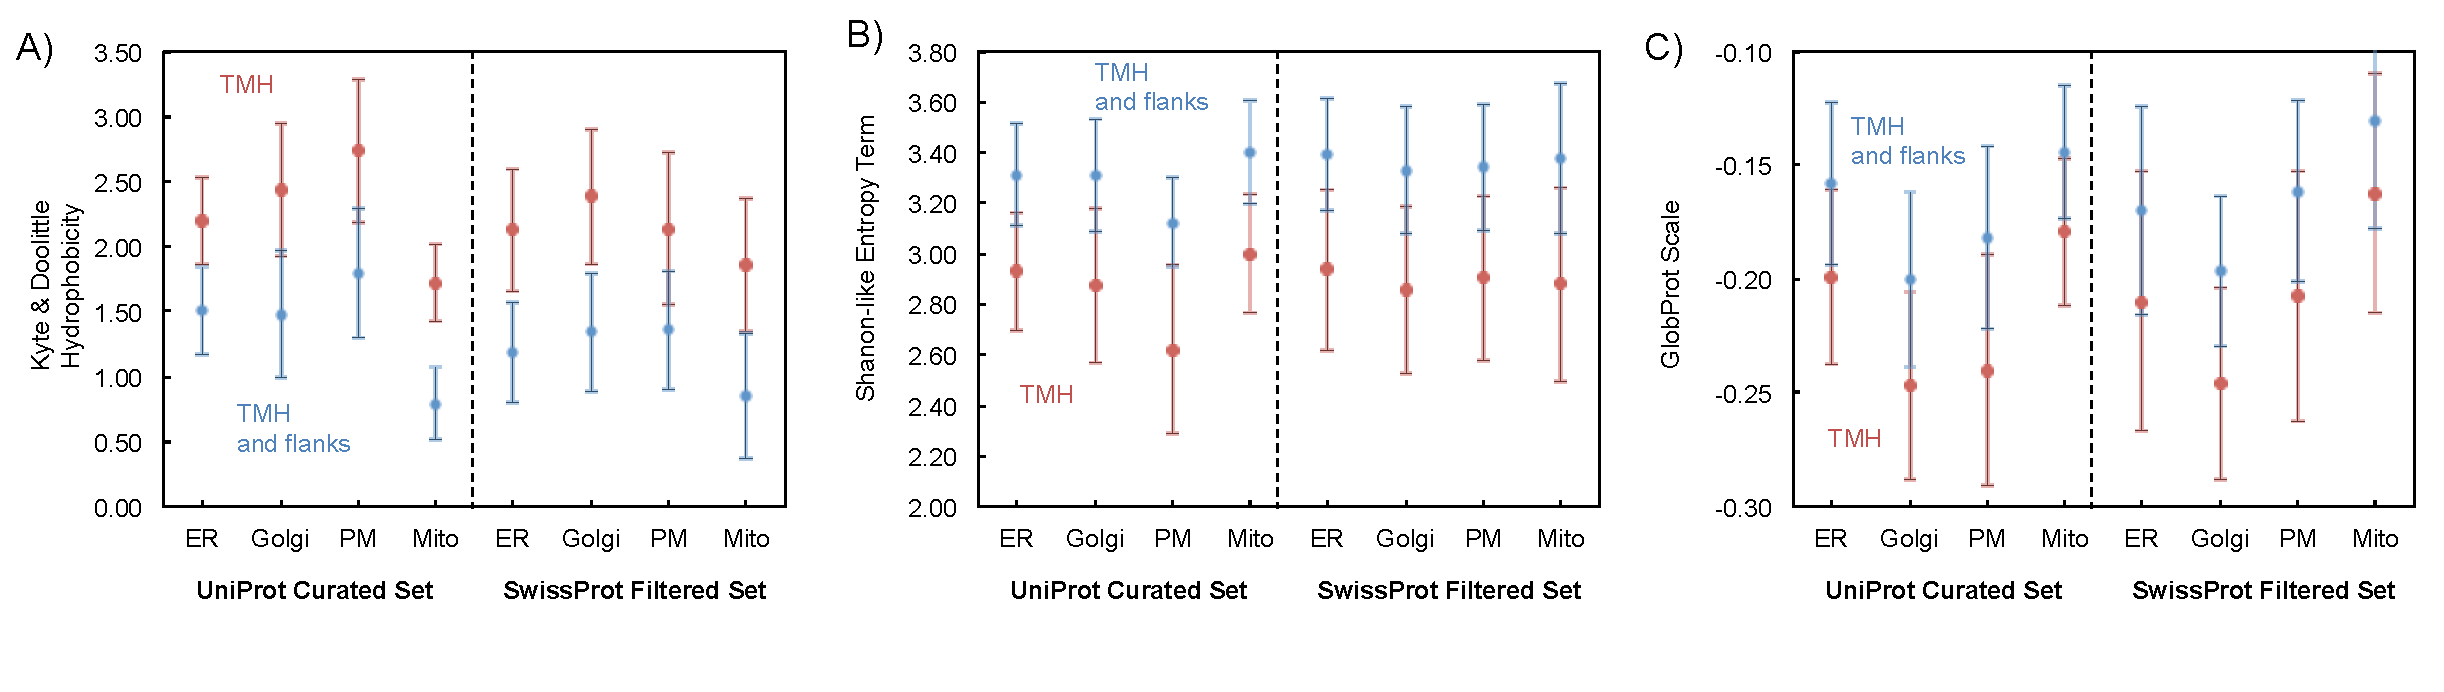
\includegraphics[width=1\textwidth]{TA_chapter/organelle-averages}
\captionof{figure}[Average sequence-based biochemical values of organelle datasets from UniProt manually curated set and SwissProt automatically filtered dataset.]
{\textbf{Average sequence-based biochemical values of organelle datasets from UniProt manually curated set and SwissProt automatically filtered dataset.}

A) The average hydrophobicity values from the Kyte \& Doolittle scale~\cite{Kyte1982}, B) the average information entropy~\cite{Shannon1948} (see methods) for both the \gls{tmh} and the \gls{tmh}$\pm$5 residues.
Values are shown for both the UniProt manually curated set and the SwissProt filtered set.
In the UniProt manually curated set we compare \gls{ta} proteins from the~\gls{er} (N=400) to the Golgi (N=82), the~\gls{pm} (N=37), and the mitochondria (N=401).
For the SwissProt filtered set we compare \gls{ta} proteins from the~\gls{er} (N=98) to the Golgi (N=82), the~\gls{pm} (N=157), and the mitochondria (N=65).
Error bars are shown at $\pm 1 \sigma$ from the mean of the respective dataset.
}

\label{fig:average_organelle_factors_ta}
\end{figure}




\begin{table}[htbp]
\centering
\captionof{table}[Statistical comparisons between TMH sequences from organelles in the UniProt Curated Dataset.]
{\textbf{Statistical comparisons between TMH sequences from organelles in the UniProt Curated Dataset.}
Here, we compare a organelle subsets from the UniProt curated dataset of \gls{ta} proteins.
We compare \gls{er} (N=397) to Golgi (N=83), \gls{pm} (N=31), and the mitochondria (N=426).
The hydrophobicity was predicted as the mean average of the values of the sequences of the \gls{tmh}, as well another group including up to $\pm$5 flanking residues, since predicting the boundary of \gls{tmh}s is difficult, according to the Kyte \& Doolittle hydrophobicity scale~\cite{Kyte1982}.
The linguistic information entropy was calculated according to the methods section~\cite{Shannon1948}.
The Test column refers to the statistical score obtained from the test; H statistic for the Kruskal Wallis (KW), the KS statistic for the Kolmogorov Smirnov test (KS), and the t-statistic for the student's T-test (T-test).
$P$ is the P-value of that statistical score.
$B$ refers to the Bahadur slope, an interpretation of the P-value that accounts for the sample size powering the test~\cite{Bahadur1967, Bahadur1971}.}
	\tiny

	\begin{tabular}{clrrrrrrrrr}
				&       & \multicolumn{3}{c}{ER and Golgi} & \multicolumn{3}{c}{ER and PM} & \multicolumn{3}{c}{ER and mito} \\
				&       & \multicolumn{1}{l}{Test} & \multicolumn{1}{l}{P} & \multicolumn{1}{l}{B} & \multicolumn{1}{l}{Test} & \multicolumn{1}{l}{P} & \multicolumn{1}{l}{B} & \multicolumn{1}{l}{Test} & \multicolumn{1}{l}{P} & \multicolumn{1}{l}{B} \\
	\multirow{3}[0]{*}{Hydrophobicity of TMH } &  Kruskal-Wallis & 21.83 & 2.98E-06 & 2.66E-02 & 28.53 & 9.21E-08 & 3.80E-02 & 377.02 & 5.54E-84 & 2.34E-01 \\
				&  Kolmogorov-Smirnov & 0.34  & 1.61E-07 & 3.27E-02 & 0.57  & 5.32E-09 & 4.47E-02 & 0.67  & 4.22E-82 & 2.28E-01 \\
				&  Student's T-test & -6.45 & 2.72E-10 & 4.61E-02 & -8.86 & 2.30E-17 & 8.99E-02 & 23.53 & 6.58E-94 & 2.61E-01 \\
	\multirow{3}[0]{*}{... and flanks} &  Kruskal-Wallis & 0.21  & 6.48E-01 & 9.07E-04 & 17.53 & 2.83E-05 & 2.46E-02 & 490.46 & 1.13E-108 & 3.03E-01 \\
				&  Kolmogorov-Smirnov & 0.19  & 1.10E-02 & 9.44E-03 & 0.50  & 4.69E-07 & 3.42E-02 & 0.82  & 5.58E-123 & 3.43E-01 \\
				&  Student's T-test & 0.32  & 7.48E-01 & 6.07E-04 & -4.85 & 1.75E-06 & 3.11E-02 & 34.60 & 2.19E-162 & 4.53E-01 \\
	\multirow{3}[0]{*}{Sequence Entropy of TMH } &  Kruskal-Wallis & 4.66  & 3.09E-02 & 7.28E-03 & 27.54 & 1.54E-07 & 3.68E-02 & 24.03 & 9.48E-07 & 1.69E-02 \\
				&  Kolmogorov-Smirnov & 0.24  & 4.78E-04 & 1.60E-02 & 0.46  & 4.20E-06 & 2.91E-02 & 0.18  & 2.10E-06 & 1.59E-02 \\
				&  Student's T-test & 3.22  & 1.37E-03 & 1.38E-02 & 6.42  & 3.71E-10 & 5.10E-02 & -4.55 & 6.28E-06 & 1.46E-02 \\
	\multirow{3}[0]{*}{... and flanks} &  Kruskal-Wallis & 0.52  & 4.70E-01 & 1.58E-03 & 19.50 & 1.01E-05 & 2.70E-02 & 40.11 & 2.40E-10 & 2.70E-02 \\
				&  Kolmogorov-Smirnov & 0.13  & 2.06E-01 & 3.31E-03 & 0.41  & 7.97E-05 & 2.22E-02 & 0.23  & 5.53E-10 & 2.60E-02 \\
				&  Student's T-test & 1.08  & 2.82E-01 & 2.65E-03 & 4.47  & 1.00E-05 & 2.70E-02 & -5.84 & 7.51E-09 & 2.28E-02 \\
	\end{tabular}%
					\label{table:organellesuniprotstats}
	\end{table}%

In the UniProt curated list, there are clear hydrophobic differences between all the \gls{tmh} datasets excluding flanks ($P<2.98E-6$) which as a trend becomes less clear when considering the \gls{tmh}$\pm$5 flanking residues except for mitochondria which increases in significance when considering the flanks also (Table~\ref{table:organellesuniprotstats}).
The \gls{er} and mitochondrial tests are very significant ($P<4.22E-82$).
Consistently the Bahadur slope is at least an order of magnitude greater in the \gls{er} and mitochondrial comparison than for the other considerations, so these differences cannot be accounted for by the larger sample size.

Information entropy has been known to identify cryptic function in \gls{tmh}s when considered along with hydrophobicity \cite{Wong2011, Wong2012}.
In terms of information entropy, there is a marked decrease in entropy in the \gls{pm} subset (mean entropy = 3.15 in the \gls{tmh}, 2.67 including $\pm$5 flanking residues) from the UniProt curated dataset compared to the other organelle datasets (entropy $>$ 3.29 and $>$ 2.85 including the flanks).
However this stark difference between \gls{tmh}s from \gls{pm} bound \gls{ta} proteins and the other organelle datasets cannot be observed in the SwissProt set (Figure~\ref{fig:average_organelle_factors_ta}).

No clear significances can be observed for the information entropy ($P>6.33E-2$).
This is unsurprising given that the hydrophobic nature of the \gls{tmh}s demands that certain residues must be over-represented, which lowers the information entropy.
In this case, we have a highly hydrophobic set, the \gls{pm} UniProt set, which likely contains a higher proportion of the most hydrophobic residues.
As a trend the information entropy mirrors the hydrophobicity albeit with less range between dataset means (2.67-3.15 in the \gls{tmh} for information entropy, 1.72-2.74 for hydrophobicity)(Figure~\ref{fig:average_organelle_factors_ta}).


	\begin{table}[htbp]
	\centering
	\captionof{table}[Statistical comparisons between TMH sequences from organelles in the SwissProt Filtered Dataset.]
	{\textbf{Statistical comparisons between TMH sequences from organelles in the SwissProt Filtered Dataset.}
	Here, we compare a organelle subsets from the SwissProt automatically filtered dataset of \gls{ta} proteins.
	We compare \gls{er} (N=98) to Golgi (N=82), \gls{pm} (N=157), and the mitochondria referred to as ``mito'' (N=65).
	The hydrophobicity was predicted as the mean average of the values of the sequences of the \gls{tmh}, as well another group including up to $\pm$5 flanking residues, since predicting the boundary of \gls{tmh}s is difficult, according to the Kyte \& Doolittle hydrophobicity scale~\cite{Kyte1982}.
	Disorder was calculated in the same way using the GlobProt scale \cite{Linding2003}.
	The linguistic information entropy was calculated according to the methods section~\cite{Shannon1948}.
	The Test column refers to the statistical score obtained from the test; H statistic for the Kruskal Wallis (KW), the KS statistic for the Kolmogorov Smirnov test (KS), and the t-statistic for the student's T-test (T-test).
	$P$ is the P-value of that statistical score.
	$B$ refers to the Bahadur slope, an interpretation of the P-value that accounts for the sample size powering the test~\cite{Bahadur1967, Bahadur1971}.}
		\tiny
		% Table generated by Excel2LaTeX from sheet 'SwissProt filtered species'

		%\begin{tabular}{clrrrrrrrrr}
		 \begin{tabular}{ccccccccccc}
								&       & \multicolumn{3}{c}{ER and Golgi} & \multicolumn{3}{c}{ER and PM} & \multicolumn{1}{l}{ER and mito} &       &  \\
								&       & \multicolumn{1}{l}{Test} & \multicolumn{1}{l}{$P$} & \multicolumn{1}{l}{$B$} & \multicolumn{1}{l}{Test} & \multicolumn{1}{l}{$P$} & \multicolumn{1}{l}{$B$} & \multicolumn{1}{l}{Test} & \multicolumn{1}{l}{$P$} & \multicolumn{1}{l}{$B$} \\

		\midrule
		\multirow{3}[0]{*}{TMH Hydrophobicity} &  KW & 11.96 & 5.43E-4 & 4.18E-2 & 0.02  & 8.77E-1 & 5.14E-4 & 8.46  & 3.64E-3 & 3.45E-2 \\
								&  KS & 0.27  & 1.98E-3 & 3.46E-2 & 0.08  & 8.48E-1 & 6.44E-4 & 0.27  & 4.62E-3 & 3.30E-2 \\
								&  T-test & -3.47 & 6.50E-4 & 4.08E-2 & -0.17 & 8.67E-1 & 5.60E-4 & 3.45  & 7.24E-4 & 4.44E-2 \\
		\midrule
		\multirow{3}[0]{*}{... including flanks} &  KW & 5.92  & 1.50E-2 & 2.33E-2 & 9.14  & 2.50E-3 & 2.35E-2 & 26.42 & 2.75E-7 & 9.27E-2 \\
								&  KS & 0.21  & 2.85E-2 & 1.98E-2 & 0.26  & 4.88E-4 & 2.99E-2 & 0.43  & 4.93E-7 & 8.91E-2 \\
								&  T-test & -2.52 & 1.25E-2 & 2.43E-2 & -3.09 & 2.23E-3 & 2.40E-2 & 4.95  & 1.87E-6 & 8.09E-2 \\
	  \midrule

		\multirow{3}[0]{*}{TMH entropy} &  KW & 2.96  & 8.56E-2 & 1.37E-2 & 0.66  & 4.17E-1 & 3.43E-3 & 0.69  & 4.05E-1 & 5.54E-3 \\
								&  KS & 0.13  & 4.32E-1 & 4.66E-3 & 0.10  & 5.27E-1 & 2.51E-3 & 0.18 & 1.40E-1 & 1.20E-2 \\
								&  T-test & 1.58  & 1.15E-1 & 1.20E-2 & 0.79  & 4.32E-1 & 3.29E-3 & 1.03 & 3.06E-1 & 7.26E-3 \\
		\midrule
		\multirow{3}[0]{*}{... including flanks} &  KW & 2.62  & 1.06E-1 & 1.25E-2 & 2.87  & 9.04E-2 & 9.42E-3 & 0.05 & 8.31E-1 & 1.14E-3 \\
								&  KS & 0.15  & 2.48E-1 & 7.75E-3 & 0.17  & 6.56E-2 & 1.07E-2 & 0.21 & 6.33E-2 & 1.69E-2 \\
								&  T-test & 1.84  & 6.75E-2 & 1.50E-2 & 1.66  & 9.84E-2 & 9.09E-3 & 0.42 & 6.72E-1 & 2.44E-3 \\
		\end{tabular}%
						\label{table:organellesswissstats}
		\end{table}%

Similarly, in the SwissProt filtered dataset the mean \gls{tmh} hydrophobicity for mitochondria is the lowest at 1.9, but it appears to be the Golgi apparatus that is the peak at 2.4.
In the SwissProt dataset, when we compare each subset of only the \gls{tmh} to the \gls{er} subset, we find significance between the \gls{er} and the Golgi ($P<1.98E-3$), and the \gls{er} and the mitochondria ($P<4.62E-3$), however the \gls{er} and \gls{pm} are more similar considering the Bahadur values are $<6.44E-4$, two orders of magnitude smaller that the other sets (Bahadur values $>3.3E-2$) (Table \ref{table:organellesswissstats}).
When we take into account the flanks, the \gls{er} and \gls{pm} dataset can be distinguished ($P<2.50E-3$), however as a trend the other two comparisons, \gls{er} and Golgi becomes less significant, and \gls{er} and mitochondria become more significant.

The linguistic information entropy of the \gls{tmh} string as well as the GlobProt disorder were also examined.
Significance was found in disorder when comparing \gls{tmh} between \gls{er} and Golgi ($P<5.01E-4$) and the \gls{pm} ($P<2.87E-6$)(Table \ref{table:organellesswissstats}), but there was no observable difference between the \gls{er} and \gls{pm}.
No significance was observed in any consideration of the information entropy, but similarly to the UniProt subset, as a trend the entropy mirrors the hydrophobicity (Figure \ref{fig:average_organelle_factors_ta}).

Whilst we expect to see hydrophobic adaptations of \gls{tmh} to the membrane environment at both a species and organelle level, we only observe such differences at the organelle level.
% Are the organelle membrane more compositionally different than species?

ADD HEATMAPS HERE

\subsection{More annotation is required to identify chaperone-specific factors.}

\subsection{Spontaneous Insertion May Be Achieved by Polar Strips in the TMH of Tail Anchored Proteins}

The \gls{tmh} of cytochrome b5 and PTP1b are among the most hydrophobic of the \gls{ta} proteins and in theory misses the $\Delta$G requirements of a \gls{tmh} \cite{Rabu2008, Rabu2009}.
Indeed the \gls{tmh} is not trivial to predict and is not found in either datasets prepared herein.
Strucural modelling and analysis thereof reveals features that may explain the ``missing hydrophobicity''~\cite{Hessa2005, Hedin2010, Hessa2007, Ojemalm2012} of these particular \gls{tmh}s.

The electrostatic surfaces are proto-typical of a \gls{tmh} anchor with large ``positive-inside'' patches \cite{VonHeijne1989, Andersson1992, Sharpe2010, Baeza-Delgado2013, Pogozheva2013, Baker2017} and a strong ``negative-outside'' charge \cite{Baker2017}(Figure \ref{fig:cytb5-biochemistry}C).
Once in the membrane, this may allow it to be an effective anchor despite such poor hydrophobicity since it satisfies electrostatic coupling to the membrane potential.

Furthermore is the question of overcoming the unfavourable interaction most \gls{tmh}s would face when coming into contact with the highly polar membrane interface.
We observe a highly conserved strip of relatively polar / non-hydrophobic residues on one side of the \gls{tmh} core (in cytochrome b5 these are N112, P116, A120, A124 Y127, and R128 whilst in PTP1b these are R430, N434, Y426, T422, and T419) which would not be as repulsed by the interfacial environment (Figure \ref{fig:cytb5-biochemistry}).
Scrambling the \gls{tmh} sequence whilst maintaining the same hydrophobicity reduces the insertion potential \cite{Brambillasca2006}; there is more to it than hydrophobicity alone.
It becomes apparent that the 3D arrangment of these relatively polar \gls{tmh} residues is conserved and is probably the key to spontaneous insertion of \gls{tmh}s.

\begin{figure}[!ht]
\centering
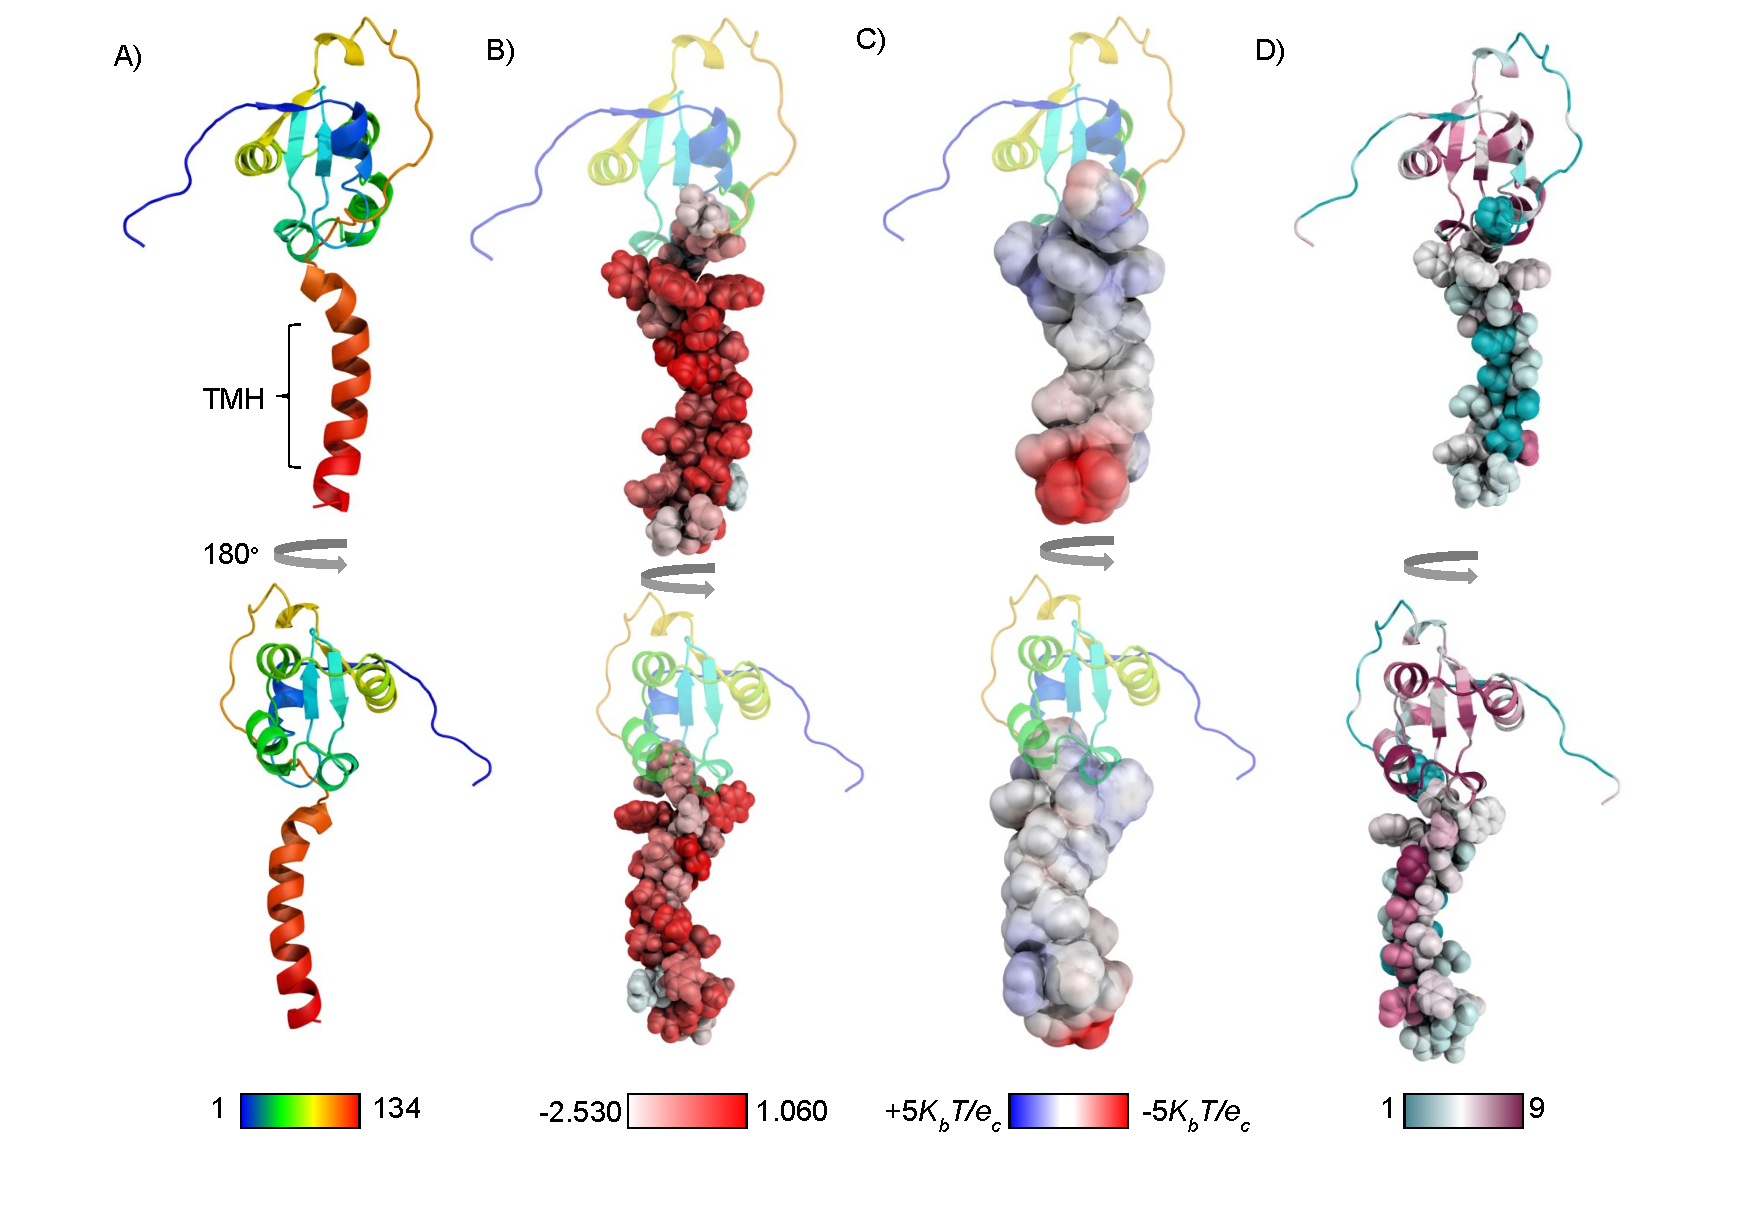
\includegraphics[width=1\textwidth]{TA_chapter/cytb5-biochemistry}
		\captionof{figure}[Structural biochemical analysis of a homology model of cytochrome b5.]{\textbf{Structural biochemical analysis of a homology model of cytochrome b5.}
		(A) The secondary structure of the protein coloured from the N terminus in blue to the C terminus in red coloured through the rainbow according to the residue number.
		(B) The hydrophobicity of the \gls{tmh} from white representing relatively polar residues to red showing relatively hydrophobic residues \cite{Eisenberg1984}.
		(C) The electrostatic surface with a threshold of $\pm5$ KT/e calculated by APBS in PyMol \cite{Baker2001}.
		Red patches are negatively charged whilst blue are positively charged.
		(D) The consurf scores on a scale of 1-9 (all residues had sufficient data) \cite{Ashkenazy2010}. Purple represents the the most conserved whilst blue is the least.
		Note the correlation between the highly and modestly conserved \gls{tmh} residues and the relatively polar residues.
		Another observable feature is the very strong ``positive inside'' \cite{VonHeijne1989, Andersson1992, Sharpe2010, Baeza-Delgado2013, Pogozheva2013} and ``negative outside'' features which are associated with anchorage \cite{Baker2017}.
}

\label{fig:cytb5-biochemistry}
\end{figure}


\begin{figure}[!ht]
\centering
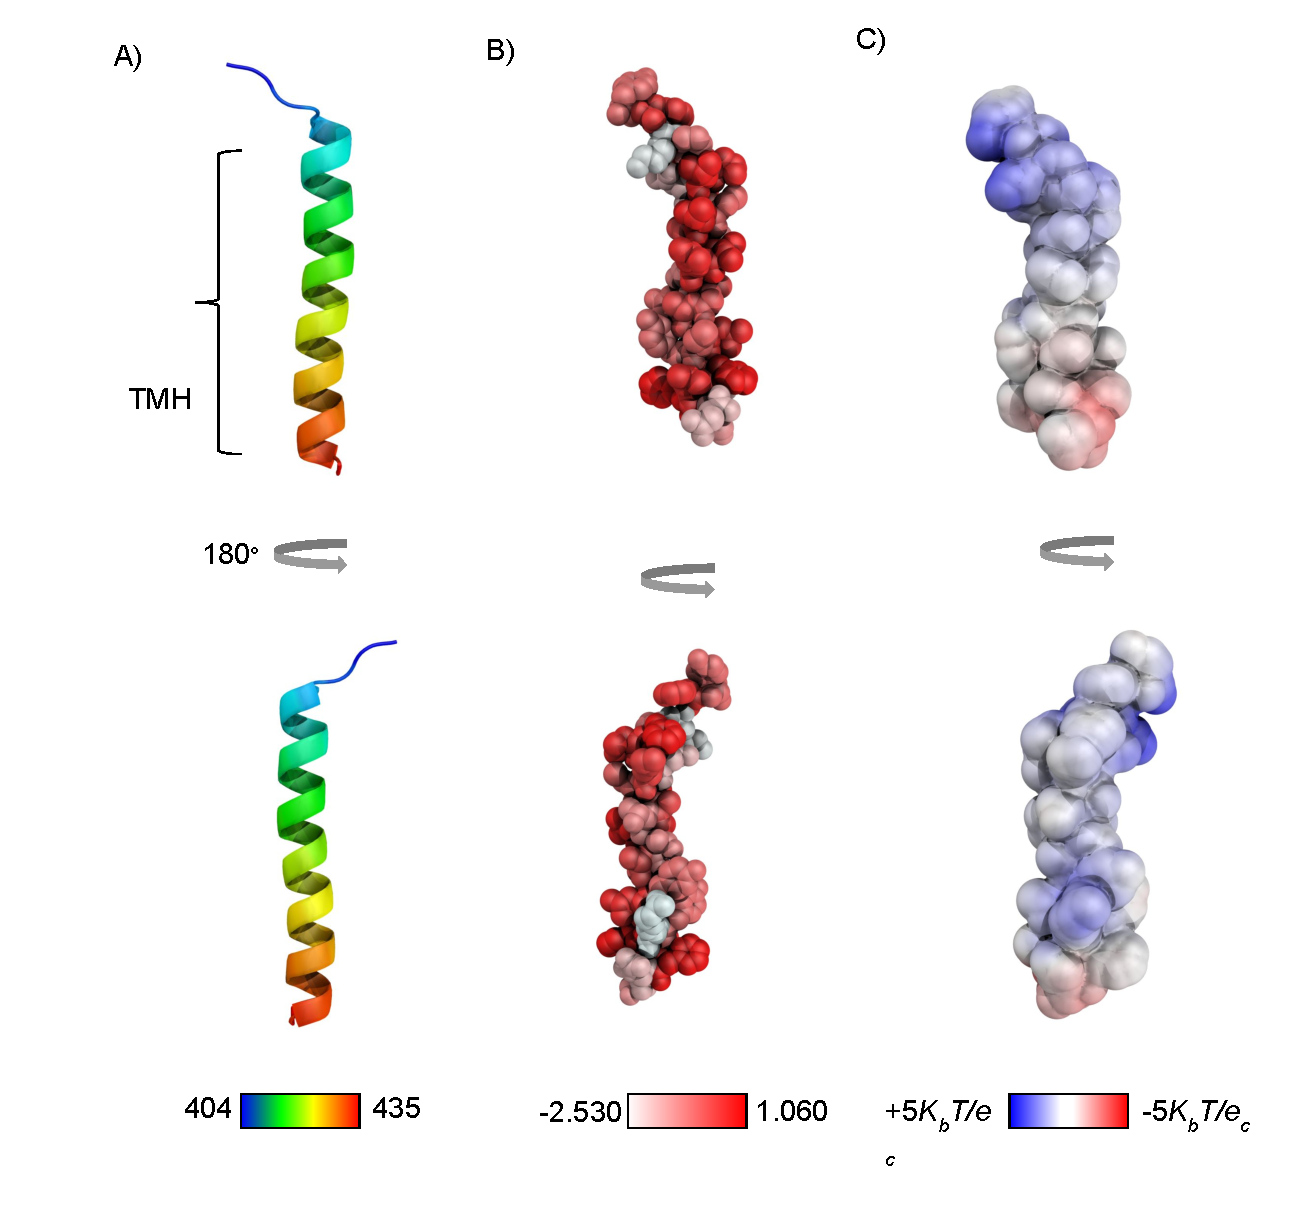
\includegraphics[width=1\textwidth]{TA_chapter/ptp1b-biochemistry}
		\captionof{figure}[Structural biochemical analysis of a homology model of PTP 1b.]{\textbf{Structural biochemical analysis of a homology model of PTP 1b.}
		(A) The secondary structure of the protein coloured from the N terminus in blue to the C terminus in red coloured through the rainbow according to the residue number.
		(B) The hydrophobicity of the \gls{tmh} from white representing relatively polar residues to red showing relatively hydrophobic residues \cite{Eisenberg1984}.
		(C) The electrostatic surface with a threshold of $\pm5$ KT/e calculated by APBS in PyMol \cite{Baker2001}.
		Red patches are negatively charged whilst blue are positively charged.
		Note the one hydrophobic face of the \gls{tmh}, and the opposing relatively polar face.
		Another observable feature the ``positive inside'' \cite{VonHeijne1989, Andersson1992, Sharpe2010, Baeza-Delgado2013, Pogozheva2013} and ``negative outside'' features which are associated with anchorage \cite{Baker2017}.
}

\label{fig:ptp1b-biochemistry}
\end{figure}

\section{Discussion}

\subsection{Adaptations and targetting factors of TMHs in tail-anchored proteins.}

We expect to see evolutionary adaptations of \gls{tmh} hydrophobicity to species specific membranes, even within eukaryotes~\cite{Baker2017, Sharpe2010}.
In this study using both a manually curated dataset from UniProt, and an automatically filtered list using SwissProt annotation, we do not observe any strong differences.
Why would we assume a stronger adaptation to organelles than to species?
Since we could not scrutinise a difference in the species, the strong hydrophobic differences between \gls{tmh}s from different organelles may not be solely accounted for by adaptation to the different membrane compositions.
Given the large biochemical distinction between \gls{ta} proteins with different terminal destinations, it is possible to conclude that \gls{tmh}s contain necessary, yet cryptic, biological factors that play a role in their targeting.
It is indeed possible that our observations are adaptations to the membrane environment, and this would not be unreasonable, except that \gls{ta} proteins would be expected to experience similar adaptations at a species level, for which at th  is sample size such an effect is unobservable.
This is almost certainly aided by other factors and is part of a system with several redundant mechanisms.

This could indeed be a cryptic functional similarity to the signal anchored proteins.
Signal anchored proteins contain a single hydrophobic segment that serves as both a mitochondrial targeting signal and a membrane anchor.
Interestingly, these proteins, along with some tail-anchored proteins, have been shown to be able to spontaneously insert into the membrane independently from the translocon~\cite{Elisa2012, Lan2000, Colombo2009}.

\subsection{Possible explanations for spontaneous insertion.}


\chapter{A novel GPI lipid anchor categorised} %Perhaps this will be for a later date!
\section{Abstract}
\section{Introduction}
\section{Methods}
\section{Results}


\chapter{The Good, the Bad, and the Ugly Helices} %Perhaps this will be for a later date!
\section{Abstract}
\section{Introduction}
\section{Methods}
\section{Results}

\chapter{Conclusions}
\sloppy
\section{Outlook}
\subsection{The hydrophobicity\---sequence complexity continuum}
We hypothesize that the hydrophobicity\---sequence complexity continuum contains nuanced codes for different functions and that such differentiation of sequence and structural properties will allow assignment to these varying functions.  Additionally, we suggest probing functional classification of yet uncharacterized membrane proteins by similarities of combinations of complex TM sets to well studied membrane proteins and finding those classes of TM proteins where this principle is most directly applicable.


% This would be better at the begining so that before we get started, let's print the glossaries.
% In order for this to work a special build sequence is needed. http://tex.stackexchange.com/a/46732/42423
\printglossary[type=\acronymtype,title=Abbreviations]
\printglossary[title=Nomenclature] % Uncomment this line to use the nomenclature section.

%This line prints the bibliography ;)
%One of the references has a "-" in the wrong place and screws up the Bibliography. %the planque reference is messed up. It may need changing with every bib.tex update unless the permannet record is changed.
\printbibliography[title={Bibliography}]

% Uncomment the following THREE lines if you do have an Appendix
%\appendix
%\chapter{}
%.........

\end{document}
